\documentclass[a4paper]{jarticle}
\usepackage[dvipdfmx]{graphicx}
\usepackage{ascmac,epic,eepic,itembbox}
\setlength{\topmargin}{-0.8cm}
\setlength{\oddsidemargin}{0.0cm}
\setlength{\textwidth}{16cm}
\setlength{\textheight}{22.4cm}
\newcommand{\R}{\mbox{\boldmath $R$}}
\newcommand{\vx}{\mbox{\boldmath $x$}}
\newcommand{\vy}{\mbox{\boldmath $y$}}
\newcommand{\va}{\mbox{\boldmath $a$}}
\newcommand{\vr}{\mbox{\boldmath $r$}}
\newcommand{\vf}{\mbox{\boldmath $f$}}
\newcommand{\vb}{\mbox{\boldmath $b$}}
\newcommand{\vc}{\mbox{\boldmath $c$}}
\newcommand{\vu}{\mbox{\boldmath $u$}}
\newcommand{\vz}{\mbox{\boldmath $z$}}
\newcommand{\ve}{\mbox{\boldmath $e$}}
\newcommand{\vv}{\mbox{\boldmath $v$}}
\newcommand{\vzero}{\mbox{\boldmath $0$}}
\newcommand{\vd}{\mbox{\boldmath $d$}}
\newcommand{\vxi}{\mbox{\boldmath $\xi$}}
\newcommand{\vZ}{\mbox{\boldmath $Z$}^{n \times n}}
\newcommand{\vepsilon}{\mbox{\boldmath $\varepsilon$}}
\newcommand{\namelistlabel}[1]{\mbox{#1}\hfill}
\newenvironment{namelist}[1]{%
\begin{list}{}
  {\let\makelabel\namelistlabel
  \settowidth{\labelwidth}{#1}
  \setlength{\leftmargin}{1.1\labelwidth}}
}{%
\end{list}}
\makeatletter
\@addtoreset{equation}{section}
\def\theequation{\thesection.\arabic{equation}}
\makeatother

\title{Lis ユーザガイド日本語版}
\author{}
\date{}
\begin{document}

\vspace*{4cm}
\begin{flushleft}
{\Large Lis ユーザガイド}\\
バージョン 2.0.33
\end{flushleft}

\vspace*{2cm}
\begin{figure}[h]

\includegraphics[scale=0.7]{irises_korin.eps}
\end{figure}

\vspace*{2cm}
\begin{flushleft}
{\large The Scalable Software Infrastructure
Project\\
{\tt http://www.ssisc.org/}}\\
\end{flushleft}

\vspace*{5mm}
\thispagestyle{empty}

\newpage
\begin{flushleft}
{\small
Copyright \copyright\ 2005 The Scalable Software Infrastructure Project,
supported by ``Development of Software Infrastructure for Large Scale
Scientific Simulation'' Team, CREST, JST.

Akira Nishida, CREST team director, JST.

All rights reserved.

\vspace*{5mm}
 Redistribution and use in source and binary forms, with or without
 modification, are permitted provided that the following conditions are
 met:

 1. Redistributions of source code must retain the above copyright
 notice, this list of conditions and the following disclaimer.

 2. Redistributions in binary form must reproduce the above copyright
 notice, this list of conditions and the following disclaimer in the
 documentation and/or other materials provided with the distribution.

 3. Neither the name of the project nor the names of its contributors
 may be used to endorse or promote products derived from this software
 without specific prior written permission.

\vspace*{5mm}
 THIS SOFTWARE IS PROVIDED BY THE SCALABLE SOFTWARE INFRASTRUCTURE
 PROJECT ``AS IS'' AND ANY EXPRESS OR IMPLIED WARRANTIES, INCLUDING, BUT
 NOT LIMITED TO, THE IMPLIED WARRANTIES OF MERCHANTABILITY AND FITNESS
 FOR A PARTICULAR PURPOSE ARE DISCLAIMED. IN NO EVENT SHALL THE SCALABLE
 SOFTWARE INFRASTRUCTURE PROJECT BE LIABLE FOR ANY DIRECT, INDIRECT,
 INCIDENTAL, SPECIAL, EXEMPLARY, OR CONSEQUENTIAL DAMAGES (INCLUDING,
 BUT NOT LIMITED TO, PROCUREMENT OF SUBSTITUTE GOODS OR SERVICES; LOSS
 OF USE, DATA, OR PROFITS; OR BUSINESS INTERRUPTION) HOWEVER CAUSED AND
 ON ANY THEORY OF LIABILITY, WHETHER IN CONTRACT, STRICT LIABILITY, OR
 TORT (INCLUDING NEGLIGENCE OR OTHERWISE) ARISING IN ANY WAY OUT OF THE
 USE OF THIS SOFTWARE, EVEN IF ADVISED OF THE POSSIBILITY OF SUCH
 DAMAGE.

\vfill
表紙: 尾形光琳. 燕子花図. 1705年頃. 根津美術館所蔵.
}
\end{flushleft}
\thispagestyle{empty}

\newpage
\pagenumbering{roman}
\tableofcontents

\setcounter{section}{0}
\pagenumbering{arabic}

\newpage
\section*{バージョン 1.0 からの変更点}
\begin{enumerate}
\item double-double型4倍精度演算に対応.
\item Fortranコンパイラに対応.
\item Autotoolsに対応.
\item 
\begin{enumerate}
\item ソルバの構造を変更.
\item 関数{\tt lis\_matrix\_create()}, {\tt lis\_vector\_create()}の引数を変更.
\item コマンドラインオプションの記法を変更.
\end{enumerate}
\end{enumerate}

\section*{バージョン 1.1 からの変更点}
\begin{enumerate}
\item 標準固有値問題に対応.
\item 64ビット整数型に対応.
\item 
\begin{enumerate}
\item 関数{\tt lis\_output\_residual\_history()}, 
      {\tt lis\_get\_residual\_history()}の名称をそれぞれ\\
      {\tt lis\_solver\_output\_rhistory()}, {\tt lis\_solver\_get\_rhistory()}に変更.
\item Fortranインタフェース{\tt lis\_vector\_set\_value()},
      {\tt lis\_vector\_get\_value()}の配列起点を1に変更.
\item Fortranインタフェース{\tt lis\_vector\_set\_size()}の配列起点を1に変更.
\item 演算精度に関するオプションの名称を {\tt -precision}から {\tt -f}に変更.
\end{enumerate}
\item 関数{\tt lis\_solve\_kernel()}の仕様を{\tt lis\_solve\_execute()}で計算
      された残差を返すよう変更. 
\item 整数型の仕様を変更. 
\begin{enumerate}
\item Cプログラムにおける整数型を{\tt LIS\_INT}に変更. 
      {\tt LIS\_INT}の既定値は{\tt int}. プリプロセッサマクロ
      {\tt \_LONGLONG}が定義された場合には, {\tt long long int}に置き換えられる. 
\item Fortranプログラムにおける整数型を{\tt LIS\_INTEGER}に変更. 
      {\tt LIS\_INTEGER}の既定値は{\tt integer}. 
      プリプロセッサマクロ{\tt LONGLONG}が定義された場合には, 
      {\tt integer*8}に置き換えられる. 
\end{enumerate}
\item 行列格納形式CRS (Compressed Row Storage), CCS (Compressed Column Storage)
      の名称をそれぞれCSR (Compressed Sparse Row), CSC (Compressed Sparse Column)
      に変更. 
\item 関数{\tt lis\_get\_solvername()}, {\tt lis\_get\_preconname()}, 
      {\tt lis\_get\_esolvername()}の名称をそれぞれ\\
      {\tt lis\_solver\_get\_solvername()}, 
      {\tt lis\_solver\_get\_preconname()}, 
{\tt lis\_esolver\_get\_esolvername()}に変更.
\end{enumerate}

\section*{バージョン 1.2 からの変更点}
\begin{enumerate}
\item nmakeに対応.  
\item ファイル{\tt lis\_config\_win32.h}の名称を{\tt lis\_config\_win.h}
      に変更.
\item 行列格納形式JDS (Jagged Diagonal Storage)の名称をJAD (Jagged Diagonal)
      に変更. 
\item 関数{\tt lis\_fscan\_double()}, {\tt lis\_bswap\_double()}の
      名称をそれぞれ{\tt lis\_fscan\_scalar()}, \\
      {\tt lis\_bswap\_scalar()}に変更.
\end{enumerate}

\section*{バージョン 1.3 からの変更点}
\begin{enumerate}
\item long double型4倍精度演算に対応.
\item Fortranでのポインタ操作に対応.  
\item 構造体{\tt LIS\_SOLVER}, {\tt LIS\_ESOLVER}のメンバ{\tt residual}の名称を{\tt rhistory}に変更.
\item 構造体{\tt LIS\_SOLVER}, {\tt LIS\_ESOLVER}のメンバ{\tt iters}, 
      {\tt iters2}の名称をそれぞれ{\tt iter}, {\tt iter2}に変更. 
\item 関数{\tt lis\_solver\_get\_iters()}, {\tt lis\_solver\_get\_itersex()}, 
      {\tt lis\_esolver\_get\_iters()}, \\
      {\tt lis\_esolver\_get\_itersex()}の名称をそれぞれ
      {\tt lis\_solver\_get\_iter()}, {\tt lis\_solver\_get\_iterex()}, 
      {\tt lis\_esolver\_get\_iter()}, {\tt lis\_esolver\_get\_iterex()}に変更.
\item 構造体{\tt LIS\_SOLVER}, {\tt LIS\_ESOLVER}のメンバ{\tt *times}の名称をそれぞれ{\tt *time}に変更. 
\item 構造体{\tt LIS\_VECTOR}にメンバ{\tt intvalue}を追加. 
\item 関数{\tt lis\_output\_vector*()}, {\tt lis\_output\_mm\_vec()}の仕様を整数値を格納できるよう変更. 
\item 関数{\tt lis\_matrix\_scaling*()}の名称をそれぞれ
      {\tt lis\_matrix\_scale*()}に変更.
\item 関数{\tt lis\_array\_dot2()}, {\tt lis\_array\_invGauss()}の名称をそれぞれ
      {\tt lis\_array\_dot()}, {\tt lis\_array\_ge()}に変更.
\end{enumerate}

\section*{バージョン 1.4 からの変更点}
\begin{enumerate}
\item 配列操作に対応.
\item 前処理とソルバの分離に対応.
\item 関数{\tt lis\_array\_qr()}の仕様をQR法の反復回数及び誤差を返すよう変更. 
\item 関数{\tt lis\_array\_matvec2()}, {\tt lis\_array\_matmat2()}の名称をそれぞれ
  {\tt lis\_array\_matvec\_ns()}, \\
  {\tt lis\_array\_matmat\_ns()}に変更.
\item プリプロセッサマクロ{\tt \_LONGLONG}, {\tt LONGLONG}の名称をそれぞれ
      {\tt \_LONG\_\_LONG}, {\tt LONG\_\_LONG}に変更.
\end{enumerate}

\section*{バージョン 1.5 からの変更点}
\begin{enumerate}
\item 複素数演算に対応.
\end{enumerate}

\section*{バージョン 1.6 からの変更点}
\begin{enumerate}
\item 一般化固有値問題に対応.
\item GCC libquadmathに対応.  
\item 固有値解法のシフト量の符号を慣例に合わせて変更.
\item {\tt lis\_matrix\_shift\_diagonal()}, {\tt lis\_vector\_shift()}, {\tt lis\_array\_shift()}のシフト量の符号をそれぞれ変更. 
\end{enumerate}

\section*{バージョン 1.7 からの変更点}
\begin{enumerate}
\item マルチステップ線型方程式解法に対応.
\item オプション {\tt -ssor\_w}及び {\tt -hybrid\_w}の名称を {\tt -ssor\_omega}及び {\tt -hybrid\_omega}にそれぞれ変更.  
\end{enumerate}

\section*{バージョン 1.8 からの変更点}
\begin{enumerate}
\item 線型方程式解法を複素演算向けに一般化.
\item 非対称固有値問題に対応.
\item エルミート内積の定義$(x,y)=y^{H}x$を$(x,y)=x^{H}y$に変更.
\item $A^T$に関する関数
      {\tt lis\_lis\_matvect*()}, 
      {\tt lis\_lis\_array\_matvect*()}, 
      {\tt lis\_matrix\_solvet*()}, \\
      {\tt lis\_psolvet*()}の名称と定義を, $A^H$に関する
      {\tt lis\_lis\_matvech*()}, 
      {\tt lis\_lis\_array\_matvech*()}, \\  
      {\tt lis\_matrix\_solveh*()}, 
      {\tt lis\_psolveh*()}にそれぞれ変更.
\item 関数{\tt lis\_matrix\_shift\_general()}の名称を{\tt lis\_matrix\_shift\_matrix()}に変更. 
\end{enumerate}

\newpage
\section{はじめに}
Lis (Library of Iterative Solvers for linear systems, 発音は[lis])は, 
偏微分方程式の数値計算に現れる離散化された線型方程式 
\[
Ax = b
\]
及び固有値問題
\[
Ax = \lambda Bx
\]
を解くための並列反復法ソフトウェアライブラリである\cite{nishida1}. 
対応する線型方程式解法, 固有値解法の一覧を表\ref{tab:solvers}-\ref{tab:esolvers}, 
前処理を表\ref{tab:precon}に示す. 
また行列格納形式の一覧を表\ref{tab:storage}に示す. 

\begin{table}[htb]
\begin{minipage}[t]{0.30\textwidth}
\caption{線型方程式解法} 
\vspace*{1mm}
\label{tab:solvers}
\hbox to\hsize{\hfil
\begin{tabular}{l|l}\hline\hline
CG\cite{hestenes,lanczos1} & CR\cite{hestenes} \\ 
BiCG\cite{fletcher,joly,pocock} & BiCR\cite{sogabe09} \\
CGS\cite{sonneveld}     & CRS\cite{abe02} \\
BiCGSTAB\cite{bicgstab} & BiCRSTAB\cite{abe02} \\
GPBiCG\cite{zhang}      & GPBiCR\cite{abe02} \\
BiCGSafe\cite{fujino01} & BiCRSafe\cite{fujino02} \\
BiCGSTAB(l)\cite{bicgstabl} & TFQMR\cite{tfqmr} \\
Jacobi\cite{jacobi}     & Orthomin(m)\cite{orthomin} \\
Gauss-Seidel\cite{gauss,seidel} & GMRES(m)\cite{gmres} \\
SOR\cite{young,frankel} & FGMRES(m)\cite{fgmres} \\
IDR(s)\cite{idrs}       & MINRES\cite{minres} \\
COCG\cite{cocg}         & COCR\cite{cocr} \\
\hline         
\end{tabular}
\hfil}
\end{minipage}
\hspace*{13mm}
\begin{minipage}[t]{0.30\textwidth}
\caption{固有値解法} 
\vspace*{1mm}
\label{tab:esolvers}
\hbox to\hsize{\hfil
\begin{tabular}{l}\hline\hline
Power\cite{power} \\
Inverse\cite{inverse} \\
Rayleigh Quotient\cite{rayleigh} \\
CG\cite{knyazev} \\
CR\cite{suetomi} \\
Subspace\cite{rutishauser} \\
Lanczos\cite{lanczos2} \\
Arnoldi\cite{arnoldi} \\
\hline         
\end{tabular}
\hfil}
\end{minipage}
\newline
\begin{minipage}[t]{0.30\textwidth}
\caption{前処理} 
\vspace*{1mm}
\label{tab:precon}
\hbox to\hsize{\hfil
\begin{tabular}{l}\hline\hline
Jacobi\cite{axelsson} \\
SSOR\cite{axelsson} \\
ILU(k)\cite{gustafsson,nakajima} \\
ILUT\cite{ilut,ITSOL} \\
Crout ILU\cite{ITSOL,iluc} \\
I+S\cite{kohno01} \\
SA-AMG\cite{fujii01}  \\
Hybrid\cite{abe01} \\
SAINV\cite{bridson01}  \\
Additive Schwarz\cite{chan,dryja} \\
ユーザ定義 \\
\hline         
\end{tabular}
\hfil}
\end{minipage}
\hspace*{-4mm}
\begin{minipage}[t]{0.30\textwidth}
\caption{行列格納形式} 
\vspace*{1mm}
\label{tab:storage}
\hbox to\hsize{\hfil
\begin{tabular}{ll}\hline\hline
Compressed Sparse Row & (CSR) \\
Compressed Sparse Column & (CSC) \\
Modified Compressed Sparse Row & (MSR) \\
Diagonal &(DIA) \\
Ellpack-Itpack Generalized Diagonal &(ELL) \\
Jagged Diagonal &(JAD) \\
Block Sparse Row & (BSR) \\
Block Sparse Column &(BSC) \\
Variable Block Row &(VBR) \\
Coordinate & (COO) \\
Dense &	(DNS) \\
\hline         
\end{tabular}
\hfil}
\end{minipage}
\end{table}

\newpage
\section{導入}
本節では, 導入, 検証の手順について述べる. 

\subsection{システム要件}
Lisの導入にはCコンパイラが必要である. 
また, Fortranインタフェースを使用する場合はFortranコンパイラ, 
AMG前処理ルーチンを使用する場合はFortran 90コンパイラが必要
である. 並列計算環境では, OpenMPライブラリ\cite{OpenMP}またはMPI-1
ライブラリ\cite{MPI}を使用する\cite{kota1,kota2}. 
データの入出力には, Harwell-Boeing 
形式\cite{duff92}, Matrix Market形式\cite{matrixmarket}が利用可能である. 
表\ref{platforms}に主な動作確認環境を示す
 (表\ref{targetoption}も参照のこと). 

\begin{table}[htbp]
\caption{主な動作確認環境}
\label{platforms}
\begin{center}
{\small
 \begin{tabular}{l|l}
\hline
\multicolumn{1}{c|}{Cコンパイラ (必須) } & \multicolumn{1}{c}{OS} \\
\hline
Intel C/C++ Compiler 7.0, 8.0, 9.1, 10.1, 11.1, 12.1, 14.0, 16.0, 17.0, 18.0, 19.0 & Linux \\
                                                     & Windows  \\
\hline
IBM XL C/C++ V7.0, 9.0                     & AIX   \\
                                           & Linux \\
\hline
Sun WorkShop 6, Sun ONE Studio 7,          & Solaris \\
Sun Studio 11, 12                          &         \\
\hline
PGI C++ 6.0, 7.1, 10.5, 16.10              & Linux \\
\hline
gcc 3.3, 4.4, 5.4, 6.4, 8.2, 9.3, 10.2     & Linux \\
                                           & macOS \\
                                           & Windows \\
\hline
Clang 3.3, 3.4, 3.7, 5.0, 6.0, 7.0, 8.0, 9.0, 10.0 & macOS \\
                                           & FreeBSD \\
\hline
Microsoft Visual C++ 2008, 2010, 2012, 2013, 2015, 2017, 2019 & Windows \\
\hline
\hline
\multicolumn{1}{c|}{Fortranコンパイラ (オプション) } & \multicolumn{1}{c}{OS} \\
\hline
Intel Fortran Compiler 8.1, 9.1, 10.1, 11.1, 12.1, 14.0, 16.0, 17.0, 18.0, 19.0 & Linux \\
                                                  & Windows  \\
\hline
IBM XL Fortran V9.1, 11.1                  & AIX     \\
                                           & Linux   \\
\hline
Sun WorkShop 6, Sun ONE Studio 7,          & Solaris \\
Sun Studio 11, 12                          &         \\
\hline
PGI Fortran 6.0, 7.1, 10.5, 16.10          & Linux \\
\hline
g77 3.3                                    & Linux \\
gfortran 4.4, 5.4, 6.4, 8.2, 10.1          & macOS \\
                                           & Windows \\
\hline
\end{tabular}
}
\end{center}
\end{table} 

\subsection{UNIX及び互換システムへの導入}
\subsubsection{アーカイブの展開}
次のコマンドを入力し, アーカイブを展開する. \verb|($VERSION)|はバージョンを示す. \\
\verb&      > unzip lis-($VERSION).zip &\\
これにより, ディレクトリ{\tt lis-(\$VERSION)}に
図\ref{listargz}に示すサブディレクトリが作成される. 

\begin{figure}[htbp]
\begin{center}
\begin{verbatim}
lis-($VERSION)
 + config
 |  設定ファイル
 + doc
 |  説明書
 + graphics
 |  描画用サンプルファイル
 + include
 |  ヘッダファイル
 + src
 |  ソースファイル
 + test
 |  検証プログラム
 + win
    Windowsシステム用設定ファイル
\end{verbatim}
\end{center}
\caption{{\tt lis-(\$VERSION).zip}のファイル構成}
\label{listargz}
\end{figure}

\subsubsection{ソースツリーの設定}
ディレクトリ{\tt lis-(\$VERSION)}において次のコマンドを実行し, ソースツリーを設定する. 
\begin{itemize}
\item 既定の設定を使用する場合 : \verb&      > ./configure&
\item 導入先を指定する場合 :   \verb&      > ./configure --prefix=<install-dir>&
\end{itemize}
表\ref{configoption}に主な設定オプションを示す. 
また, 表\ref{targetoption}に\verb+TARGET+として指定できる主な計算機環境を示す. 
\begin{table}[htbp]
\caption{主な設定オプション (一覧は {\tt ./configure --help}を参照) }
\label{configoption}
\begin{center}
\begin{tabular}{|l|l|}
\hline
\verb+--enable-omp+      & OpenMPライブラリを使用\\ \hline
\verb+--enable-mpi+      & MPIライブラリを使用\\ \hline
\verb+--enable-fortran+  & FORTRAN 77互換インタフェースを使用\\ \hline
\verb+--enable-f90    +  & Fortran 90互換インタフェースを使用\\ \hline
\verb+--enable-saamg+    & SA-AMG前処理を使用\\ \hline
\verb+--enable-quad+     & double-double型4倍精度演算を使用\\ \hline
\verb+--enable-longdouble+ & long double型4倍精度演算を使用\\ \hline
\verb+--enable-longlong+ & 64ビット整数型を使用\\ \hline
\verb+--enable-complex+  & スカラ型として複素数型を使用\\ \hline
\verb+--enable-debug+    & デバッグモードを使用\\ \hline
\verb+--enable-shared+   & 動的リンクを使用\\ \hline
\verb+--enable-gprof+    & プロファイラを使用\\ \hline
\verb+--disable-test+    & 検証プログラムを作成しない\\ \hline    
\verb+--prefix=<install-dir>+    & 導入先を指定\\ \hline
\verb+TARGET=<target>+    & 計算機環境を指定\\ \hline
\verb+CC=<c_compiler>+    & Cコンパイラを指定\\ \hline
\verb+CFLAGS=<c_flags>+    & Cコンパイラオプションを指定\\ \hline
\verb+F77=<f77_compiler>+    & FORTRAN 77コンパイラを指定\\ \hline
\verb+F77FLAGS=<f77_flags>+    & FORTRAN 77コンパイラオプションを指定\\ \hline
\verb+FC=<f90_compiler>+    & Fortran 90コンパイラを指定\\ \hline
\verb+FCFLAGS=<f90_flags>+    & Fortran 90コンパイラオプションを指定\\ \hline
\verb+LDFLAGS=<ld_flags>+    & リンクオプションを指定\\ \hline
\end{tabular}
\end{center}
\end{table}
\begin{table}[htbp]
\caption{TARGETの例 (詳細は{\tt lis-(\$VERSION)/configure.ac}を参照) }
\label{targetoption}
\begin{center}
\begin{tabular}{|l|l|}
\hline
\verb+<target>+           & 等価なオプション \\ \hline
\verb+cray_xt3_cross+     & \verb+./configure CC=cc FC=ftn CFLAGS="-O3 -B -fastsse -tp k8-64"+ \\
                          & \verb+  FCFLAGS="-O3 -fastsse -tp k8-64 -Mpreprocess" FCLDFLAGS="-Mnomain"+\\
                          & \verb+  ac_cv_sizeof_void_p=8 cross_compiling=yes+\\
                          & \verb+  ax_f77_mangling="lower case, no underscore, extra underscore"+ \\ \hline
\verb+fujitsu_fx10_cross+ & \verb|./configure CC=fccpx FC=frtpx CFLAGS="-Kfast,ocl,preex"| \\
                          & \verb+  FCFLAGS="-Kfast,ocl,preex -Cpp -fs" FCLDFLAGS="-mlcmain=main"+\\
                          & \verb+  ac_cv_sizeof_void_p=8 cross_compiling=yes+\\
                          & \verb+  ax_f77_mangling="lower case, underscore, no extra underscore"+ \\ \hline
\verb+hitachi_sr16k+      & \verb|./configure CC=cc FC=f90 CFLAGS="-Os -noparallel"| \\
                          & \verb+  FCFLAGS="-Oss -noparallel" FCLDFLAGS="-lf90s"+ \\
                          & \verb+  ac_cv_sizeof_void_p=8+ \\
                          & \verb+  ax_f77_mangling="lower case, underscore, no extra underscore" + \\ \hline
\verb+ibm_bgl_cross+      & \verb+./configure CC=blrts_xlc FC=blrts_xlf90+ \\
                          & \verb+  CFLAGS="-O3 -qarch=440d -qtune=440 -qstrict"+ \\
                          & \verb+  FCFLAGS="-O3 -qarch=440d -qtune=440 -qsuffix=cpp=F90"+ \\
                          & \verb+  ac_cv_sizeof_void_p=4 cross_compiling=yes+\\
                          & \verb+  ax_f77_mangling="lower case, no underscore, no extra underscore"+ \\ \hline
\verb+intel_mic_cross+    & \verb+./configure CC=icc F77=ifort FC=ifort+ \\
                          & \verb+  MPICC=mpiicc MPIF77=mpiifort MPIFC=mpiifort+ \\
                          & \verb+  CFLAGS="-mmic" FFLAGS="-mmic" FCFLAGS="-mmic"+ \\
                          & \verb+  LDFLAGS="-mmic" FCLDFLAGS="-mmic" cross_compiling=yes+ \\
                          & \verb+  host=x86_64-pc-linux-gnu host_alias=x86_64-linux-gnu+ \\
                          & \verb+  host_cpu=x86_64 host_os=linux-gnu host_vendor=pc+ \\
                          & \verb+  target=k1om-mpss-linux-gnu target_alias=k1om-mpss-linux+ \\
                          & \verb+  target_cpu=k1om target_os=linux-gnu target_vendor=mpss+ \\ \hline
\verb+nec_sx9_cross+      & \verb|./configure CC=sxmpic++ FC=sxmpif90 AR=sxar RANLIB=true | \\
                          & \verb+  ac_cv_sizeof_void_p=8 ax_vector_machine=yes cross_compiling=yes+ \\ 
                          & \verb+  ax_f77_mangling="lower case, no underscore, extra underscore"+ \\ \hline
\end{tabular}
\end{center}
\end{table}

\subsubsection{実行ファイルの生成}
ディレクトリ{\tt lis-(\$VERSION)}において次のコマンドを入力し, 実行ファイルを生成する.\\
 \verb+      > make +\\
実行ファイルが正常に生成されたかどうかを確認するには, 
ディレクトリ{\tt lis-(\$VERSION)}において次のコマンドを入力し, ディレク
 トリ{\tt lis-(\$VERSION)/test}に生成された実行ファイルを用いて検証を行う. \\
 \verb+      > make check+\\
このコマンドでは, Matrix Market形式のファイル{\tt test/testmat.mtx}
から行列, ベクトルデータを読み込み, BiCG法を用いて線型方程式$Ax=b$の解を
求める. 以下にSGI Altix 3700上での実行結果を示す. 
なおオプション {\tt --enable-omp}と {\tt --enable-mpi}は組み合わせて
使用することができる. 
\begin{itembox}[l]{既定}
\begin{minipage}{10cm}
\begin{verbatim}
matrix size = 100 x 100 (460 nonzero entries)

initial vector x      : all components set to 0
precision             : double
linear solver         : BiCG
preconditioner        : none
convergence condition : ||b-Ax||_2 <= 1.0e-12 * ||b-Ax_0||_2
matrix storage format : CSR
linear solver status  : normal end

BiCG: number of iterations = 15 (double = 15, quad = 0)
BiCG: elapsed time         = 5.178690e-03 sec.
BiCG:   preconditioner     = 1.277685e-03 sec.
BiCG:     matrix creation  = 1.254797e-03 sec.
BiCG:   linear solver      = 3.901005e-03 sec.
BiCG: relative residual    = 6.327297e-15
\end{verbatim}
\end{minipage}
\end{itembox}
\begin{itembox}[l]{ {\tt --enable-omp}}
 \begin{minipage}{10cm}
 \begin{verbatim}
max number of threads = 32
number of threads = 2
matrix size = 100 x 100 (460 nonzero entries)

initial vector x      : all components set to 0
precision             : double
linear solver         : BiCG
preconditioner        : none
convergence condition : ||b-Ax||_2 <= 1.0e-12 * ||b-Ax_0||_2
matrix storage format : CSR
linear solver status  : normal end

BiCG: number of iterations = 15 (double = 15, quad = 0)
BiCG: elapsed time         = 8.960009e-03 sec.
BiCG:   preconditioner     = 2.297878e-03 sec.
BiCG:     matrix creation  = 2.072096e-03 sec.
BiCG:   linear solver      = 6.662130e-03 sec.
BiCG: relative residual    = 6.221213e-15
\end{verbatim}
\end{minipage}
\end{itembox}
\begin{itembox}[l] {\tt --enable-mpi}
 \begin{minipage}{10cm}
 \begin{verbatim}
number of processes = 2
matrix size = 100 x 100 (460 nonzero entries)

initial vector x      : all components set to 0
precision             : double
linear solver         : BiCG
preconditioner        : none
convergence condition : ||b-Ax||_2 <= 1.0e-12 * ||b-Ax_0||_2
matrix storage format : CSR
linear solver status  : normal end

BiCG: number of iterations = 15 (double = 15, quad = 0)
BiCG: elapsed time         = 2.911400e-03 sec.
BiCG:   preconditioner     = 1.560780e-04 sec.
BiCG:     matrix creation  = 1.459997e-04 sec.
BiCG:   linear solver      = 2.755322e-03 sec.
BiCG: relative residual    = 6.221213e-15
\end{verbatim}
\end{minipage}
\end{itembox}

\subsubsection{導入}
ディレクトリ{\tt lis-(\$VERSION)}において次のコマンドを入力し, 導入先のディレクトリにファイルを複製する.\\
 \verb+      > make install+\\ 
これにより, ディレクトリ{\tt (\$INSTALLDIR)}に以下のファイルが複製される.

\begin{verbatim}
($INSTALLDIR)
 +bin
 |   +lsolve esolve esolver gesolve gesolver hpcg_kernel hpcg_spmvtest spmvtest*
 +include
 |   +lis_config.h lis.h lisf.h
 +lib
 |   +liblis.a
 +share
     +doc/lis examples/lis man
\end{verbatim}
{\tt lis\_config.h}はライブラリを生成する際に, また{\tt lis.h}はC, {\tt lisf.h}はFortranで
ライブラリを使用する際に必要なヘッダファイルである. {\tt liblis.a}は生成された
ライブラリである. 
ライブラリが正常に導入されたかどうかを確認するには, 
ディレクトリ{\tt lis-(\$VERSION)}において次のコマンドを入力し, ディレク
トリ{\tt examples/lis}に生成された実行ファイルを用いて検証を行う. \\
 \verb+      > make installcheck+ \\
{\tt examples/lis}下の{\tt test1}, {\tt etest5}, {\tt etest5b}, {\tt getest5}, {\tt getest5b}, 
{{\tt test3b}, {{\tt spmvtest3b}は, 
{\tt lsolve}, {\tt esolve}, {\tt esolver}, {\tt gesolve}, {\tt gesolver}, 
{\tt hpcg\_kernel}, {\tt hpcg\_spmvtest}の別名で{\tt (\$INSTALLDIR)/bin}に複製される.
{\tt examples/lis/spmvtest*}も, それぞれ{\tt (\$INSTALLDIR)/bin}に
複製される.

{\tt (\$INSTALLDIR)}に複製されたファイルを削除するには,
次のコマンドを入力する. \\
 \verb+      > make uninstall+\\
{\tt lis-(\$VERSION)}に生成されたライブラリ, 及び実行ファイルを削除するには,
次のコマンドを入力する. \\
 \verb+      > make clean+\\
生成された設定ファイルを合わせて削除するには,
次のコマンドを入力する. \\
 \verb+      > make distclean+

\subsection{Windowsシステムへの導入}
適当なツールを用いてアーカイブを展開した後, 
Microsoft Build Engineを使用する場合は, 
ディレクトリ{\tt lis-(\$VERSION)\textbackslash win}において次のコマンドを入力し, 
設定ファイル{\tt Makefile}を生成する 
(詳細は{\tt configure.bat --help}を参照). \\
 \verb+      > configure.bat+\\
{\tt Makefile}の既定値は{\tt Makefile.in}で定義される. 
実行ファイルを生成するには, {\tt lis-(\$VERSION)\textbackslash win}
において次のコマンドを入力する. \\
 \verb+      > nmake+\\
実行ファイルが正常に生成されたかどうかを確認するには, 
次のコマンドを入力し, 生成された実行ファイルを用いて検証を行う. \\
 \verb+      > nmake check+\\
生成されたライブラリ, 実行ファイル, ヘッダファイル, 及びPDF文書は,
以下のコマンドにより\\
{\tt (\$INSTALLDIR)\textbackslash lib}, 
{\tt (\$INSTALLDIR)\textbackslash bin},
{\tt (\$INSTALLDIR)\textbackslash include}, 
及び{\tt (\$INSTALLDIR)\textbackslash doc}
にそれぞれ格納される. \\
 \verb+      > nmake install+\\
{\tt (\$INSTALLDIR)}に複製されたファイルを削除するには,
次のコマンドを入力する. \\
 \verb+      > nmake uninstall+\\
{\tt (\$INSTALLDIR)\textbackslash win}に生成されたライブラリ,
及び実行ファイルを削除するには,次のコマンドを入力する. \\
 \verb+      > nmake clean+\\
生成された設定ファイルを合わせて削除するには,次のコマンドを入力する. \\
 \verb+      > nmake distclean+

UNIX互換環境を使用する場合は前節を参照のこと. 

\subsection{検証}
検証プログラムは{\tt lis-(\$VERSION)/test}に格納される. 
\subsubsection{test1}
ディレクトリ{\tt lis-(\$VERSION)/test}において\\
 \verb+      > test1 matrix_filename rhs_setting solution_filename rhistory_filename [options]+\\
と入力すると, {\tt matrix\_filename}から行列データを読み込み, 
線型方程式$Ax=b$を{\tt options}で指定された解法で解く. また, 
解を拡張Matrix Market形式で{\tt solution\_filename}に, 
残差履歴をPLAIN形式で{\tt rhistory\_filename}に書き出す 
(付録\ref{sec:matinp}を参照). 
入力可能な行列データ形式は拡張Matrix Market形式, Harwell-Boeing形式のいずれかである. 
{\tt rhs\_setting}には
\begin{namelist}{XXXXXXXXXXXXXXXXXXXX}
\item[0] 行列データファイルに含まれる右辺ベクトルを用いる
\item[1] $b = (1,\dots,1)^T$を用いる
\item[2] $b = A \times (1,\dots,1)^T$を用いる
\item[rhs\_filename] 右辺ベクトルのファイル名
\end{namelist}
のいずれかを指定できる. {\tt rhs\_filename}はPLAIN形式, Matrix Market形式に対応する. 
{\tt test1f.F}は{\tt test1.c}のFortran版である. 

\subsubsection{test2}
ディレクトリ{\tt lis-(\$VERSION)/test}において\\
 \verb+      > test2 m n matrix_type solution_filename rhistory_filename [options]+\\
と入力すると, 2次元Laplace作用素を5点中心差分により離散化して得られる
次数$mn$の行列$A$を係数とする
線型方程式$Ax=b$を, \verb|matrix_type|で指定された行列格納形式, 
{\tt options}で指定された解法で解く. また, 
解を拡張Matrix Market形式で{\tt solution\_filename}に, 
残差履歴をPLAIN形式で{\tt rhistory\_filename}に書き出す.
右辺ベクトル$b$は解ベクトル$x$の値が
すべて$1$となるよう設定される. {\tt m}, {\tt n}は各次元の格子点数である. 
{\tt test2f.F90}は{\tt test2.c}のFortran 90版である. 

\subsubsection{test2b}
ディレクトリ{\tt lis-(\$VERSION)/test}において\\
 \verb+      > test2b m n matrix_type solution_filename rhistory_filename [options]+\\
と入力すると, 2次元Laplace作用素を9点中心差分により離散化して得られる
次数$mn$の行列$A$を係数とする
線型方程式$Ax=b$を, \verb|matrix_type|で指定された行列格納形式, 
{\tt options}で指定された解法で解く. また, 
解を拡張Matrix Market形式で{\tt solution\_filename}に, 
残差履歴をPLAIN形式で{\tt rhistory\_filename}に書き出す.
右辺ベクトル$b$は解ベクトル$x$の値がすべて$1$となるよう設定される. {\tt m}, {\tt n}は各次元の格子点数である. 

\subsubsection{test3}
ディレクトリ{\tt lis-(\$VERSION)/test}において\\
 \verb+      > test3 l m n matrix_type solution_filename rhistory_filename [options]+\\
と入力すると, 3次元Laplace作用素を7点中心差分により離散化して得られる
次数$lmn$の行列$A$を係数とする
線型方程式$Ax=b$を, \verb|matrix_type|で指定された行列格納形式, 
{\tt options}で指定された解法で解く. また, 
解を拡張Matrix Market形式で{\tt solution\_filename}に, 
残差履歴をPLAIN形式で{\tt rhistory\_filename}に書き出す.
右辺ベクトル$b$は解ベクトル$x$の値がすべて$1$となるよう
設定される. {\tt l}, {\tt m}, {\tt n}は各次元の格子点数である. 

\subsubsection{test3b}
ディレクトリ{\tt lis-(\$VERSION)/test}において\\
 \verb+      > test3b l m n matrix_type solution_filename rhistory_filename [options]+\\
と入力すると, 3次元Laplace作用素を27点中心差分により離散化して得られる
次数$lmn$の行列$A$を係数とする
線型方程式$Ax=b$を, \verb|matrix_type|で指定された行列格納形式, 
{\tt options}で指定された解法で解く. また, 
解を拡張Matrix Market形式で{\tt solution\_filename}に, 
残差履歴をPLAIN形式で{\tt rhistory\_filename}に書き出す.
右辺ベクトル$b$は解ベクトル$x$の値がすべて$1$となるよう
設定される. {\tt l}, {\tt m}, {\tt n}は各次元の格子点数である. 

\subsubsection{test3c}
ディレクトリ{\tt lis-(\$VERSION)/test}において\\
 \verb+      > test3c l m n step [options]+\\
と入力すると, 3次元Laplace作用素を7点中心差分により離散化して得られる
次数$lmn$の行列$A$を係数とする
線型方程式$Ax=b$を, {\tt options}で指定された解法で{\tt step}ステップ分解く.
右辺ベクトル$b$は解ベクトル$x$の値がすべて$1$となるよう
設定される. 行列,右辺ベクトルの値はステップ毎に更新される.
{\tt l}, {\tt m}, {\tt n}は各次元の格子点数である. 
 
\subsubsection{test4}
線型方程式$Ax=b$を指定された解法で解き, 解を標準出力に書き出す. 
行列$A$は次数$12$の3重対角行列
\[
A = 
\left(
\begin{array}{ccccc}
2 & -1 &   &  &   \\
-1 & 2 & -1 &  &   \\
  & \ddots  & \ddots  & \ddots  &   \\
  &   & -1 & 2 & -1 \\
  &   &   & -1 & 2 \\
\end{array}
\right)
\]
である. 右辺ベクトル$b$は解ベクトル$x$の値がすべて$1$となるよう
設定される. 
{\tt test4f.F}は{\tt test4.c}のFortran版である. 

\subsubsection{test5}
ディレクトリ{\tt lis-(\$VERSION)/test}において\\
 \verb+      > test5 n gamma [options]+\\
と入力すると, 
線型方程式$Ax=b$を指定された解法で解く. 
行列$A$は次数$n$のToepliz行列
\[
A = \left(
\begin{array}{cccccc}
2 & 1 &   &  &  & \\
0 & 2 & 1 &  &  & \\
\gamma & 0& 2 & 1 &  & \\
 & \ddots & \ddots & \ddots & \ddots & \\
 &  &   \gamma &0 &       2   & 1 \\
 &  &  &   \gamma & 0& 2 \\
\end{array}
\right)
\]
である. 右辺ベクトル$b$は解ベクトル$x$の値がすべて$1$となるよう
設定される. 

\subsubsection{test6}
{\tt test6.c}は{\tt test2.c}の配列版である. 
ディレクトリ{\tt lis-(\$VERSION)/test}において\\
 \verb+      > test6 m n+\\
と入力すると, 2次元Laplace作用素を5点中心差分により離散化して得られる
次数$mn$の行列$A$を係数とする線型方程式$Ax=b$を直接法で解く.
右辺ベクトル$b$は解ベクトル$x$の値が
すべて$1$となるよう設定される. {\tt m}, {\tt n}は各次元の格子点数である. 
{\tt test6f.F90}は{\tt test6.c}のFortran 90版である.

\subsubsection{test7}
ディレクトリ{\tt lis-(\$VERSION)/test}において\\
 \verb+      > test7+\\
と入力すると, 複素演算の使用例を示す.
{\tt test7f.F}は{\tt test7.c}のFortran版である.

\subsubsection{test8f}

ディレクトリ{\tt lis-(\$VERSION)/test}において\\
 \verb+      > mpiexec -n m test8f+\\
 と入力すると, Newton-Raphson法を用いて非線形偏微分方程式を解く.
Newton-Raphson法において, 前処理行列はソルバと切り離して更新される(\ref{subsec:psd}節を参照のこと).

\subsubsection{etest1}
ディレクトリ{\tt lis-(\$VERSION)/test}において\\
 \verb+      > etest1 matrix_filename evector_filename rhistory_filename [options]+\\
と入力すると, {\tt matrix\_filename}から行列データを読み込み, 
標準固有値問題$Ax=\lambda x$を{\tt options}で指定された解法で解いて, 指定され
た固有値を標準出力に書き出す. また, 対応する固有ベクトルを拡張Matrix
 Market形式で{\tt evector\_filename}に, 残差履歴をPLAIN形式で
{\tt rhistory\_filename}に書き出す. 
入力可能な行列データ形式はMatrix Market形式, もしくはHarwell-Boeing形式の
いずれかである. 
{\tt etest1f.F}は{\tt etest1.c}のFortran版である. 
複数の固有対を取得する場合は{\tt etest5}を参照のこと.

\subsubsection{getest1}
ディレクトリ{\tt lis-(\$VERSION)/test}において\\
 \verb+      > getest1 matrix_a_filename matrix_b_filename evector_filename rhistory_filename +\\
\verb+ [options]+\\
と入力すると, {\tt matrix\_a\_filename}及び{\tt matrix\_b\_filename}から
行列データを読み込み, 
一般化固有値問題$Ax=\lambda Bx$を{\tt options}で指定された解法で解いて, 指定され
た固有値を標準出力に書き出す. また, 対応する固有ベクトルを拡張Matrix
 Market形式で{\tt evector\_filename}に, 残差履歴をPLAIN形式で
{\tt rhistory\_filename}に書き出す. 
入力可能な行列データ形式はMatrix Market形式, もしくはHarwell-Boeing形式の
いずれかである. 
複数の固有対を取得する場合は{\tt getest5}を参照のこと.

\subsubsection{etest2}
ディレクトリ{\tt lis-(\$VERSION)/test}において\\
 \verb+      > etest2 m n matrix_type evector_filename rhistory_filename [options]+\\
と入力すると, 2次元Laplace作用素を5点中心差分により離散化して得られる
次数$mn$の行列$A$に関する固有値問題
$Ax=\lambda x$を, \verb|matrix_type|で指定された行列格納形式, 
{\tt options}で指定された解法で解き, 指定された固有値を標準出力に書き出す. 
また, 
対応する固有ベクトルを{\tt evector\_filename}に, 残差履歴を{\tt rhistory\_filename}に書き出す. 
{\tt m}, {\tt n}は各次元の格子点数である. 

\subsubsection{etest3}
ディレクトリ{\tt lis-(\$VERSION)/test}において\\
 \verb+      > etest3 l m n matrix_type evector_filename rhistory_filename [options]+\\
と入力すると, 3次元Laplace作用素を7点中心差分により離散化して得られる
次数$lmn$の行列$A$に関する固有値問題
$Ax=\lambda x$を, \verb|matrix_type|で指定された行列格納形式, 
{\tt options}で指定された解法で解き, 指定された固有値を標準出力に書き出す. 
また, 対応する固有ベクトルを拡張Matrix Market形式で{\tt evector\_filename}に, 
残差履歴をPLAIN形式で{\tt rhistory\_filename}に書き出す. 
{\tt l}, {\tt m}, {\tt n}は各次元の格子点数である.
複数の固有対を取得する場合は{\tt etest6}を参照のこと.

\subsubsection{etest4}
ディレクトリ{\tt lis-(\$VERSION)/test}において\\
 \verb+      > etest4 n [options]+\\
と入力すると, 固有値問題$Ax=\lambda x$を指定された解法で解き, 指定された
固有値を標準出力に書き出す. 
行列$A$は次数$n$の3重対角行列
\[
A = 
\left(
\begin{array}{ccccc}
2 & -1 &   &  &   \\
-1 & 2 & -1 &  &   \\
  & \ddots  & \ddots  & \ddots  &   \\
  &   & -1 & 2 & -1 \\
  &   &   & -1 & 2 \\
\end{array}
\right)
\]
である. 
{\tt etest4f.F}は{\tt etest4.c}のFortran版である. 

\subsubsection{etest5}
ディレクトリ{\tt lis-(\$VERSION)/test}において\\
 \verb+      > etest5 matrix_filename evalues_filename evectors_filename residuals_filename +\\
\verb+ iters_filename [options] +\\
と入力すると, {\tt matrix\_filename}から行列データを読み込み, 
標準固有値問題$Ax=\lambda x$を{\tt options}で
指定された解法で解く. 
また, オプション {\tt -ss}により指定された個数の固有値を
{\tt evalues\_filename}に, 対応する固有ベクトル, 残差ノルム及び反復回数を
{\tt evectors\_filename}, 
{\tt residuals\_filename}及び{\tt iters\_filename}に
拡張Matrix Market形式で書き出す.
入力可能な行列データ形式はMatrix Market形式, もしくはHarwell-Boeing形式の
いずれかである. 

\subsubsection{etest5b}
ディレクトリ{\tt lis-(\$VERSION)/test}において\\
 \verb+      > etest5b matrix_filename evalues_filename [options] +\\
と入力すると, {\tt matrix\_filename}から行列データを読み込み, 
標準固有値問題$Ax=\lambda x$を{\tt options}で
指定された解法で解く. 
また, オプション {\tt -ss}により指定された個数のRitz値を
{\tt evalues\_filename}に拡張Matrix Market形式で書き出す.
入力可能な行列データ形式はMatrix Market形式, もしくはHarwell-Boeing形式の
いずれかである. 

\subsubsection{getest5}
ディレクトリ{\tt lis-(\$VERSION)/test}において\\
 \verb+      > getest5 matrix_a_filename matrix_b_filename evalues_filename evectors_filename +\\
\verb+ residuals_filename iters_filename [options] +\\
と入力すると, {\tt matrix\_a\_filename}及び{\tt matrix\_b\_filename}から
行列データを読み込み, 一般化固有値問題$Ax=\lambda Bx$を{\tt options}で
指定された解法で解く.
また, オプション {\tt -ss}により指定された個数の固有値を
{\tt evalues\_filename}に, 対応する固有ベクトル, 残差ノルム及び反復回数を
{\tt evectors\_filename}, {\tt residuals\_filename}及び{\tt iters\_filename}に
拡張Matrix Market形式で書き出す. 
入力可能な行列データ形式はMatrix Market形式, もしくはHarwell-Boeing形式の
いずれかである. 

\subsubsection{getest5b}
ディレクトリ{\tt lis-(\$VERSION)/test}において\\
 \verb+      > getest5b matrix_a_filename matrix_b_filename evalues_filename [options] +\\
と入力すると, {\tt matrix\_a\_filename}及び{\tt matrix\_b\_filename}から
行列データを読み込み, 一般化固有値問題$Ax=\lambda Bx$を{\tt options}で
指定された解法で解く.
また, オプション {\tt -ss}により指定された個数のRitz値を
{\tt evalues\_filename}に拡張Matrix Market形式で書き出す. 
入力可能な行列データ形式はMatrix Market形式, もしくはHarwell-Boeing形式の
いずれかである. 

\subsubsection{etest6}
ディレクトリ{\tt lis-(\$VERSION)/test}において\\
 \verb+      > etest6 l m n matrix_type evalues_filename evectors_filename residuals_filename +\\
\verb+ iters_filename [options] +\\
と入力すると, 3次元Laplace作用素を7点中心差分により離散化して得られる
次数$lmn$の行列$A$に関する固有値問題
$Ax=\lambda x$を, \verb|matrix_type|で指定された行列格納形式, 
{\tt options}で指定された解法で解く.
また, オプション {\tt -ss}により指定された個数の固有値を
{\tt evalues\_filename}に, 対応する固有ベクトル, 残差ノルム及び反復回数を
{\tt evectors\_filename}, {\tt residuals\_filename}及び
{\tt iters\_filename}に拡張Matrix Market形式で書き出す. 
{\tt l}, {\tt m}, {\tt n}は各次元の格子点数である. 

\subsubsection{etest7}
{\tt etest7.c}は{\tt etest2.c}の配列版である. 
ディレクトリ{\tt lis-(\$VERSION)/test}において\\
 \verb+      > etest7 m n+\\
と入力すると, 2次元Laplace作用素を5点中心差分により離散化して得られる
次数$mn$の行列$A$に関する固有値問題$Ax=\lambda x$をQR法で解く. 
{\tt m}, {\tt n}は各次元の格子点数である. 

\subsubsection{spmvtest1}
ディレクトリ{\tt lis-(\$VERSION)/test}において\\
 \verb+      > spmvtest1 n iter [matrix_type]+\\
と入力すると, 1次元Laplace作用素を3点中心差分により離散化して
得られる次数$n$の行列
\[
A = 
\left(
\begin{array}{ccccc}
2 & -1 &   &  &   \\
-1 & 2 & -1 &  &   \\
  & \ddots  & \ddots  & \ddots  &   \\
  &   & -1 & 2 & -1 \\
  &   &   & -1 & 2 \\
\end{array}
\right)
\]
とベクトル$(1,\dots,1)^T$との積を
{\tt iter}で指定された回数実行し, FLOPS値を算出する. 
必要なら{\tt matrix\_type}により, 
\begin{namelist}{XXXXXXXXXXXXXXXXXXXX}
\item[0] 実行可能なすべての行列格納形式について測定する
\item[1-11] 行列格納形式の番号
\end{namelist}
のいずれかを指定する. 

\subsubsection{spmvtest2}
ディレクトリ{\tt lis-(\$VERSION)/test}において\\
 \verb+      > spmvtest2 m n iter [matrix_type]+\\
と入力すると, 2次元Laplace作用素を5点中心差分により離散化して得られる
次数$mn$の5重対角行列とベクトル
$(1,\dots,1)^T$との積を
{\tt iter}で指定された回数実行し, FLOPS値を算出する. 
必要なら{\tt matrix\_type}により, 
\begin{namelist}{XXXXXXXXXXXXXXXXXXXX}
\item[0] 実行可能なすべての行列格納形式について測定する
\item[1-11] 行列格納形式の番号
\end{namelist}
のいずれかを指定する. {\tt m}, {\tt n}は各次元の格子点数である. 

\subsubsection{spmvtest2b}
ディレクトリ{\tt lis-(\$VERSION)/test}において\\
 \verb+      > spmvtest2b m n iter [matrix_type]+\\
と入力すると, 2次元Laplace作用素を9点中心差分により離散化して得られる
次数$mn$の9重対角行列とベクトル
$(1,\dots,1)^T$との積を
{\tt iter}で指定された回数実行し, FLOPS値を算出する. 
必要なら{\tt matrix\_type}により, 
\begin{namelist}{XXXXXXXXXXXXXXXXXXXX}
\item[0] 実行可能なすべての行列格納形式について測定する
\item[1-11] 行列格納形式の番号
\end{namelist}
のいずれかを指定する. {\tt m}, {\tt n}は各次元の格子点数である. 

\subsubsection{spmvtest3}
ディレクトリ{\tt lis-(\$VERSION)/test}において\\
 \verb+      > spmvtest3 l m n iter [matrix_type]+\\
と入力すると, 3次元Laplace作用素を7点中心差分により離散化して得られる
次数$lmn$の7重対角行列とベクトル
$(1,\dots,1)^T$との積を
{\tt iter}で指定された回数実行し, FLOPS値を算出する. 
必要なら{\tt matrix\_type}により, 
\begin{namelist}{XXXXXXXXXXXXXXXXXXXX}
\item[0] 実行可能なすべての行列格納形式について測定する
\item[1-11] 行列格納形式の番号
\end{namelist}
のいずれかを指定する. {\tt l}, {\tt m}, {\tt n}は各次元の格子点数である. 

\subsubsection{spmvtest3b}
ディレクトリ{\tt lis-(\$VERSION)/test}において\\
 \verb+      > spmvtest3b l m n iter [matrix_type]+\\
と入力すると, 3次元Laplace作用素を27点中心差分により離散化して得られる
次数$lmn$の27重対角行列とベクトル
$(1,\dots,1)^T$との積を
{\tt iter}で指定された回数実行し, FLOPS値を算出する. 
必要なら{\tt matrix\_type}により, 
\begin{namelist}{XXXXXXXXXXXXXXXXXXXX}
\item[0] 実行可能なすべての行列格納形式について測定する
\item[1-11] 行列格納形式の番号
\end{namelist}
のいずれかを指定する. {\tt l}, {\tt m}, {\tt n}は各次元の格子点数である. 

\subsubsection{spmvtest4}
ディレクトリ{\tt lis-(\$VERSION)/test}において\\
 \verb+      > spmvtest4 matrix_filename_list iter [block]+\\
と入力すると, {\tt matrix\_filename\_list}の示す行列データ
ファイルリストから行列データを読み込み, 各行列とベクトル
$(1,\dots,1)^T$との積を実行可能な行列格納形式について
{\tt iter}で指定された回数実行し, FLOPS値を算出する.
入力可能な行列データ形式はMatrix Market形式, もしくはHarwell-Boeing形式の
いずれかである. 
必要なら{\tt block}により, BSR, BSC形式のブロックサイズを指定する. 

\subsubsection{spmvtest5}
ディレクトリ{\tt lis-(\$VERSION)/test}において\\
 \verb+      > spmvtest5 matrix_filename matrix_type iter [block]+\\
と入力すると, {\tt matrix\_filename}の示す行列データファイル
から行列データを読み込み, 行列とベクトル$(1,\dots,1)^T$との
積を行列格納形式{\tt matrix\_type}について{\tt iter}で
指定された回数実行し, FLOPS値を算出する. 
入力可能な行列データ形式はMatrix Market形式, もしくはHarwell-Boeing形式の
いずれかである. 
必要なら{\tt block}により, BSR, BSC形式のブロックサイズを指定する. 

\subsection{制限事項}
現バージョンには以下の制限がある. 
\begin{itemize}
\item 行列格納形式
\begin{itemize}
\item VBR形式はマルチプロセス環境では使用できない. 
\item CSR形式以外の格納形式はSA-AMG前処理では使用できない. 
\item マルチプロセス環境において必要な配列を直接定義する場合は, CSR形式
      を使用しなければならない.
      他の格納形式を使用する場合は, 関数\verb|lis_matrix_convert()|を用いて
      変換を行う. 
\end{itemize}

\item double-double型4倍精度演算(\ref{sec:quadruple}節を参照)
\begin{itemize}
\item 線型方程式解法のうち, Jacobi, Gauss-Seidel, SOR, IDR(s), COCG, COCR法では使用できない.
\item 固有値解法では使用できない.
\item Hybrid前処理での内部反復解法のうち, Jacobi, Gauss-Seidel, SOR法では使用できない.
\item I+S, SA-AMG前処理では使用できない.
\item double-double型4倍精度演算は複素演算には対応していない.
\item long-double型4倍精度演算と併用することはできない.
\end{itemize}

\item 前処理
\begin{itemize}
\item ILU(k)前処理のアルゴリズムは, ブロック対角要素を並列に分解する局所ILU前処理\cite{nakajima}に基づく. スレッド数またはプロセス数が増加するにつれて収束特性がJacobi前処理に近づく点に注意のこと.
\item Jacobi, SSOR以外の前処理が選択され, かつ行列AがCSR形式でない場合,
      前処理作成時にCSR形式の行列Aが作成される.
\item 非対称線型方程式解法としてBiCG法が選択された場合, SA-AMG前処理は使用できない.
\item SA-AMG前処理はマルチスレッド計算には対応していない.
\item SA-AMG前処理は複素演算には対応していない.   
\item SAINV前処理の前処理行列作成部分は逐次実行される.
\item ユーザ定義前処理は使用できない.
\end{itemize}

\item 固有値解法
\begin{itemize}
\item 複素固有値を計算する場合には,複素演算を有効にする必要がある. 
\end{itemize}

\end{itemize}
\vspace*{5mm}

\newpage
\section{基本操作}
本節では, ライブラリの使用方法について述べる. 
プログラムでは, 以下の処理を行う必要がある. 
\begin{itemize}
\item 初期化処理
\item 行列の作成
\item ベクトルの作成
\item ソルバ (解法の情報を格納する構造体) の作成
\item 行列, ベクトルへの値の代入
\item 解法の設定
\item 求解
\item 終了処理
\end{itemize}
また, プログラムの先頭には以下のコンパイラ指示文を記述しなければならない. 
\begin{itemize}
\item \verb+C       #include "lis.h"+
\item \verb+Fortran #include "lisf.h"+
\end{itemize}
{\tt lis.h}, {\tt lisf.h}は, 導入時に
\verb|($INSTALLDIR)/include|下に格納される. 

\subsection{初期化・終了処理}
初期化, 終了処理は以下のように記述する. 初期化処理はプログラムの最初に, 
終了処理は最後に実行しなければならない. 
\begin{itembox}[l]{C}
\small
\begin{verbatim}
 1: #include "lis.h"
 2: LIS_INT main(LIS_INT argc, char* argv[])
 3: {
 4:     lis_initialize(&argc, &argv);
 5:     ...
 6:     lis_finalize();
 7: }
\end{verbatim}
\end{itembox}
\begin{itembox}[l]{Fortran}
\small
\begin{verbatim}
 1: #include "lisf.h"
 2:      call lis_initialize(ierr) 
 3:     ...
 4:      call lis_finalize(ierr)
\end{verbatim}
\end{itembox}
\\ \\
\noindent
{\bf 初期化処理}

初期化処理を行うには, 関数
\begin{itemize}
\item \verb+C       LIS_INT lis_initialize(LIS_INT* argc, char** argv[])+
\item \verb+Fortran subroutine lis_initialize(LIS_INTEGER ierr)+
\end{itemize}
を用いる. 
この関数は, MPIの初期化, コマンドライン引数の取得等の初期化処理を行う. 

{\tt LIS\_INT}の既定値{\tt int}は, プリプロセッサマクロ
{\tt \_LONG\_\_LONG}が定義された場合には{\tt long long int}に, また
{\tt LIS\_INTEGER}の既定値{\tt integer}は, 
プリプロセッサマクロ{\tt LONG\_\_LONG}が定義された場合には
{\tt integer*8}に置き換えられる. 
\\ \\
\noindent
{\bf 終了処理}

終了処理を行うには, 関数
\begin{itemize}
\item \verb+C       LIS_INT lis_finalize()+
\item \verb+Fortran subroutine lis_finalize(LIS_INTEGER ierr)+
\end{itemize}
を用いる. 

\subsection{ベクトルの操作}
ベクトル$v$の次数を$global\_n$とする. 
ベクトル$v$を$nprocs$個のプロセスで行ブロック分割する場合の
各部分ベクトルの行数を$local\_n$とする. 
$global\_n$が$nprocs$で割り切れる場合は
$local\_n$ $=$ $global\_n$ $/$ $nprocs$となる. 
例えば, 
ベクトル$v$を(\ref{eq:vecv})式のように2プロセスで行ブロック分割する場合, 
$global\_n$と$local\_n$はそれぞれ$4$と$2$となる. 
\begin{equation}
v = 
\left(
\begin{array}{c}
0 \\
1 \\ \hline
2 \\
3  
\end{array}
\right)
\begin{array}{l}
\mbox{PE0} \\
    \\
\mbox{PE1} \\
   \\ 
\end{array}
\label{eq:vecv}
\end{equation}

(\ref{eq:vecv})式のベクトル$v$を作成する場合, 
逐次, マルチスレッド環境ではベクトル$v$そのものを, マルチプロセス環境では各プロセスに
プロセス数で行ブロック分割した
部分ベクトルを作成する. 

ベクトル$v$を作成するプログラムは以下のように記述する. ただし, マルチプロセス環境の
プロセス数は$2$とする. 
\begin{itembox}[l]{C (逐次・マルチスレッド環境)}
\small
\begin{verbatim}
 1: LIS_INT i,n;
 2: LIS_VECTOR v;
 3: n = 4;
 4: lis_vector_create(0,&v);
 5: lis_vector_set_size(v,0,n);              /* or lis_vector_set_size(v,n,0); */ 
 6:
 7: for(i=0;i<n;i++)
 8: {
 9:     lis_vector_set_value(LIS_INS_VALUE,i,(double)i,v);
10: }
\end{verbatim}
\end{itembox}
\begin{itembox}[l]{C (マルチプロセス環境)}
\small
\begin{verbatim}
 1: LIS_INT i,n,is,ie;                       /* or LIS_INT i,ln,is,ie; */
 2: LIS_VECTOR v;
 3: n = 4;                                   /* ln = 2; */
 4: lis_vector_create(MPI_COMM_WORLD,&v);
 5: lis_vector_set_size(v,0,n);              /* lis_vector_set_size(v,ln,0); */
 6: lis_vector_get_range(v,&is,&ie);
 7: for(i=is;i<ie;i++)
 8: {
 9:     lis_vector_set_value(LIS_INS_VALUE,i,(double)i,v);
10: }
\end{verbatim}
\end{itembox}
\begin{itembox}[l]{Fortran (逐次・マルチスレッド環境)}
\small
\begin{verbatim}
 1: LIS_INTEGER i,n
 2: LIS_VECTOR v
 3: n = 4
 4: call lis_vector_create(0,v,ierr)
 5: call lis_vector_set_size(v,0,n,ierr)  
 6:
 7: do i=1,n
 9:     call lis_vector_set_value(LIS_INS_VALUE,i,DBLE(i),v,ierr)
10: enddo
\end{verbatim}
\end{itembox}
\begin{itembox}[l]{Fortran (マルチプロセス環境)}
\small
\begin{verbatim}
 1: LIS_INTEGER i,n,is,ie                 
 2: LIS_VECTOR v
 3: n = 4                                   
 4: call lis_vector_create(MPI_COMM_WORLD,v,ierr)
 5: call lis_vector_set_size(v,0,n,ierr)              
 6: call lis_vector_get_range(v,is,ie,ierr)
 7: do i=is,ie-1
 8:     call lis_vector_set_value(LIS_INS_VALUE,i,DBLE(i),v,ierr);
 9: enddo
\end{verbatim}
\end{itembox}
\\ \\
\noindent
{\bf ベクトルの作成}

ベクトル$v$の作成には, 関数
\begin{itemize}
\item \verb|C       LIS_INT lis_vector_create(LIS_Comm comm, LIS_VECTOR *v)|
\item \verb|Fortran subroutine lis_vector_create(LIS_Comm comm, LIS_VECTOR v, LIS_INTEGER ierr)|
\end{itemize}
を用いる. 
{\tt comm}にはMPIコミュニケータを指定する. 逐次, マルチスレッド環境では{\tt comm}の値は無視される. 
\\ \\
\noindent
{\bf 次数の設定}

次数の設定には, 関数
\begin{itemize}
\item \verb|C       LIS_INTEGER lis_vector_set_size(LIS_VECTOR v, LIS_INT local_n,|\\
      \verb|         LIS_INT global_n)|
\item \verb|Fortran subroutine lis_vector_set_size(LIS_VECTIR v, LIS_INTEGER local_n,| \\
      \verb|         LIS_INTEGER global_n, LIS_INTEGER ierr)|
\end{itemize}
を用いる. 
$local\_n$ か $global\_n$ のどちらか一方を与えなければならない. 

逐次, マルチスレッド環境では, $local\_n$ $は$ $global\_n$に等しい.
したがって, 
\verb|lis_vector_set_size(v,n,0)|
と\verb|lis_vector_set_size(v,0,n)|は, いずれも次数$n$のベクトルを作成する.

マルチプロセス環境においては, \verb|lis_vector_set_size(v,n,0)|は
各プロセス上に次数$n$の部分ベクトルを作成する. 
一方, \verb|lis_vector_set_size(v,0,n)|は各プロセス$p$上に次数$m_p$の部分ベクトルを作成する. $m_p$はライブラリ側で決定される. 
\\ \\
\noindent
{\bf 値の代入}

ベクトル$v$の第$i$行に値を代入するには, 関数
\begin{itemize}
\item \verb|C       LIS_INT lis_vector_set_value(LIS_INT flag, LIS_INT i, LIS_SCALAR value,|\\
      \verb|         LIS_VECTOR v)|
\item \verb|Fortran subroutine lis_vector_set_value(LIS_INTEGER flag, LIS_INTEGER i,|\\
      \verb|         LIS_SCALAR value, LIS_VECTOR v, LIS_INTEGER ierr)|
\end{itemize}
を用いる. マルチプロセス環境では, 部分ベクトルの第$i$行ではなく,全体ベクトルの第$i$行を指定する. 
\verb+flag+には
\begin{description}
\item[\tt LIS\_INS\_VALUE] 挿入: $v[i] = value$
\item[\tt LIS\_ADD\_VALUE] 加算代入: $v[i] = v[i] + value$
\end{description}
のどちらかを指定する.
\\ \\
\noindent
{\bf ベクトルの複製}

既存のベクトルと同じ情報を持つベクトルを作成するには, 関数
\begin{itemize}
\item \verb|C       LIS_INT lis_vector_duplicate(LIS_VECTOR vin, LIS_VECTOR *vout)|
\item \verb|Fortran subroutine lis_vector_duplicate(LIS_VECTOR vin, LIS_VECTOR vout,|\\
      \verb|         LIS_INTEGER ierr)|
\end{itemize}
を用いる. 第1引数\verb|LIS_VECTOR vin|は\verb|LIS_MATRIX|を指定することも可能である. 
この関数はベクトルの要素の値は複製しない. 値も複製する場合は,
この関数の後に
\begin{itemize}
\item \verb|C       LIS_INT lis_vector_copy(LIS_VECTOR vsrc, LIS_VECTOR vdst)|
\item \verb|Fortran subroutine lis_vector_copy(LIS_VECTOR vsrc, LIS_VECTOR vdst, LIS_INTEGER ierr)|
\end{itemize}
を呼び出す. 
\\ \\
\noindent
{\bf ベクトルの破棄}

不要になったベクトルをメモリから破棄するには, 
\begin{itemize}
\item \verb|C       LIS_INT lis_vector_destroy(LIS_VECTOR v)|
\item \verb|Fortran subroutine lis_vector_destroy(LIS_VECTOR v, LIS_INTEGER ierr)|
\end{itemize}
を用いる. 

\subsection{行列の操作}
行列$A$の次数を$global\_n$ $\times$ $global\_n$とする. 
行列$A$を$nprocs$個のプロセスで行ブロック分割する場合の
各ブロックの行数を$local\_n$とする. 
$global\_n$が$nprocs$で割り切れる場合は
$local\_n$ $=$ $global\_n$ $/$ $nprocs$となる. 
例えば, 
行列$A$を(\ref{eq:mat})式のように2個のプロセスで行ブロック分割する場合, 
$global\_n$と$local\_n$はそれぞれ$4$と$2$となる. 
\begin{equation}
\label{eq:mat}
A = 
\left(
\begin{array}{cccc}
2 & 1 &   &    \\
1 & 2 & 1 &    \\ \hline
  & 1 & 2 & 1 \\
  &   & 1 & 2 
\end{array}
\right)
\begin{array}{l}
\mbox{PE0} \\
    \\
\mbox{PE1} \\
   \\ 
\end{array}
\end{equation}

目的の格納形式の行列を作成するには以下の3つの方法がある.\\ \\
\noindent
{\bf 方法1: ライブラリ関数を用いて目的の格納形式の配列を定義する場合}\\
(\ref{eq:mat})式の行列$A$をCSR形式で作成する場合, 
逐次, マルチスレッド環境では行列$A$そのものを, マルチプロセス環境では各プロセスに
プロセス数で行ブロック分割した
部分行列を作成する. 

行列$A$をCSR形式で作成するプログラムは以下のように記述する. 
ただし, マルチプロセス環境のプロセス数は$2$とする. 
\begin{itembox}[l]{C (逐次・マルチスレッド環境)}
\small
\begin{verbatim}
 1: LIS_INT i,n;
 2: LIS_MATRIX A;
 3: n = 4;
 4: lis_matrix_create(0,&A);
 5: lis_matrix_set_size(A,0,n);              /* or lis_matrix_set_size(A,n,0); */ 
 6: for(i=0;i<n;i++) {
 7:     if( i>0   ) lis_matrix_set_value(LIS_INS_VALUE,i,i-1,1.0,A);
 8:     if( i<n-1 ) lis_matrix_set_value(LIS_INS_VALUE,i,i+1,1.0,A);
 9:     lis_matrix_set_value(LIS_INS_VALUE,i,i,2.0,A);
10: }
11: lis_matrix_set_type(A,LIS_MATRIX_CSR);
12: lis_matrix_assemble(A);
\end{verbatim}
\end{itembox}
\begin{itembox}[l]{C (マルチプロセス環境)}
\small
\begin{verbatim}
 1: LIS_INT i,n,gn,is,ie;                 
 2: LIS_MATRIX A;
 3: gn = 4;                                  /* or n=2 */
 4: lis_matrix_create(MPI_COMM_WORLD,&A);
 5: lis_matrix_set_size(A,0,gn);             /*	lis_matrix_set_size(A,n,0); */
 6: lis_matrix_get_size(A,&n,&gn);
 7: lis_matrix_get_range(A,&is,&ie);
 8: for(i=is;i<ie;i++) {
 9:     if( i>0    ) lis_matrix_set_value(LIS_INS_VALUE,i,i-1,1.0,A);
10:     if( i<gn-1 ) lis_matrix_set_value(LIS_INS_VALUE,i,i+1,1.0,A);
11:     lis_matrix_set_value(LIS_INS_VALUE,i,i,2.0,A);
12: }
13: lis_matrix_set_type(A,LIS_MATRIX_CSR);
14: lis_matrix_assemble(A);
\end{verbatim}
\end{itembox}
\begin{itembox}[l]{Fortran (逐次・マルチスレッド環境)}
\small
\begin{verbatim}
 1: LIS_INTEGER i,n
 2: LIS_MATRIX A
 3: n = 4
 4: call lis_matrix_create(0,A,ierr)
 5: call lis_matrix_set_size(A,0,n,ierr)
 6: do i=1,n
 7:     if( i>1 ) call lis_matrix_set_value(LIS_INS_VALUE,i,i-1,1.0d0,A,ierr)
 8:     if( i<n ) call lis_matrix_set_value(LIS_INS_VALUE,i,i+1,1.0d0,A,ierr)
 9:     call lis_matrix_set_value(LIS_INS_VALUE,i,i,2.0d0,A,ierr)
10: enddo
11: call lis_matrix_set_type(A,LIS_MATRIX_CSR,ierr)
12: call lis_matrix_assemble(A,ierr)
\end{verbatim}
\end{itembox}
\begin{itembox}[l]{Fortran (マルチプロセス環境)}
\small
\begin{verbatim}
 1: LIS_INTEGER i,n,gn,is,ie                 
 2: LIS_MATRIX A
 3: gn = 4
 4: call lis_matrix_create(MPI_COMM_WORLD,A,ierr)
 5: call lis_matrix_set_size(A,0,gn,ierr)
 6: call lis_matrix_get_size(A,n,gn,ierr)
 7: call lis_matrix_get_range(A,is,ie,ierr)
 8: do i=is,ie-1
 9:     if( i>1  ) call lis_matrix_set_value(LIS_INS_VALUE,i,i-1,1.0d0,A,ierr)
10:     if( i<gn ) call lis_matrix_set_value(LIS_INS_VALUE,i,i+1,1.0d0,A,ierr)
11:     call lis_matrix_set_value(LIS_INS_VALUE,i,i,2.0d0,A,ierr)
12: enddo
13: call lis_matrix_set_type(A,LIS_MATRIX_CSR,ierr)
14: call lis_matrix_assemble(A,ierr)
\end{verbatim}
\end{itembox}
\\ \\
\noindent
{\bf 行列の作成}

行列$A$の作成には, 関数
\begin{itemize}
\item \verb|C       LIS_INT lis_matrix_create(LIS_Comm comm, LIS_MATRIX *A)|
\item \verb|Fortran subroutine lis_matrix_create(LIS_Comm comm, LIS_MATRIX A, LIS_INTEGER ierr)|
\end{itemize}
を用いる. 
{\tt comm}にはMPIコミュニケータを指定する. 逐次, マルチスレッド環境では, {\tt comm}の値は無視される. 
\\ \\
\noindent
{\bf 次数の設定}

次数の設定には, 関数
\begin{itemize}
\item \verb|C       LIS_INT lis_matrix_set_size(LIS_MATRIX A, LIS_INT local_n, LIS_INT global_n)|
\item \verb|Fortran subroutine lis_matrix_set_size(LIS_MATRIX A, LIS_INTEGER local_n,|\\
      \verb|         LIS_INTEGER global_n, LIS_INTEGER ierr)|
\end{itemize}
を用いる. 
$local\_n$ か $global\_n$ のどちらか一方を与えなければならない. 

逐次, マルチスレッド環境では, $local\_n$ $は$ $global\_n$に等しい. 
したがって, 
\verb|lis_matrix_set_size(A,n,0)|
と\verb|lis_matrix_set_size(A,0,n)|は, いずれも次数$n \times n$の行列を作成する. 

マルチプロセス環境においては, \verb|lis_matrix_set_size(A,n,0)|は各プロセス上に次数$n \times N$の部分行列を作成する. $N$は$n$の総和である. \\
一方, \verb|lis_matrix_set_size(A,0,n)|は各プロセス$p$上に次数$m_p \times n$の部分行列を作成する. $m_p$はライブラリ側で決定される. 
\\ \\
\noindent
{\bf 値の代入}

行列$A$の第$i$行第$j$列に値を代入するには, 関数
\begin{itemize}
\item \verb|C       LIS_INT lis_matrix_set_value(LIS_INT flag, LIS_INT i, LIS_INT j,|\\
      \verb|         LIS_SCALAR value, LIS_MATRIX A)|
\item \verb|Fortran subroutine lis_matrix_set_value(LIS_INTEGER flag, LIS_INTEGER i,|\\
      \verb|         LIS_INTEGER j, LIS_SCALAR value, LIS_MATRIX A, LIS_INTEGER ierr)|
\end{itemize}
を用いる. マルチプロセス環境では, 全体行列の第$i$行第$j$列を指定する. 
flagには
\begin{description}
\item[\tt LIS\_INS\_VALUE] 挿入: $A[i,j] = value$
\item[\tt LIS\_ADD\_VALUE] 加算代入: $A[i,j] = A[i,j] + value$
\end{description}
のどちらかを指定する. 
\\ \\
\noindent
{\bf 行列格納形式の設定}

行列の格納形式を設定するには, 関数
\begin{itemize}
\item \verb|C       LIS_INT lis_matrix_set_type(LIS_MATRIX A, LIS_INT matrix_type)|
\item \verb|Fortran subroutine lis_matrix_set_type(LIS_MATRIX A, LIS_INTEGER matrix_type,|\\
      \verb|         LIS_INTEGER ierr)|
\end{itemize}
を用いる. 
行列作成時の$A$の\verb|matrix_type|は\verb|LIS_MATRIX_CSR|である.
以下に対応する格納形式を示す. 
\\ \\
\begin{minipage}[t]{\textwidth}
\begin{center}
\begin{tabular}{lll}\hline\hline
格納形式  & & \verb|matrix_type| \\ \hline
Compressed Sparse Row & (CSR) & \verb={LIS_MATRIX_CSR|1}= \\
Compressed Sparse Column & (CSC) & \verb={LIS_MATRIX_CSC|2}= \\
Modified Compressed Sparse Row & (MSR) & \verb={LIS_MATRIX_MSR|3}= \\
Diagonal &(DIA) & \verb={LIS_MATRIX_DIA|4}= \\
Ellpack-Itpack Generalized Diagonal &(ELL) & \verb={LIS_MATRIX_ELL|5}= \\
Jagged Diagonal &(JAD) & \verb={LIS_MATRIX_JAD|6}= \\
Block Sparse Row & (BSR) & \verb={LIS_MATRIX_BSR|7}= \\
Block Sparse Column &(BSC) & \verb={LIS_MATRIX_BSC|8}= \\
Variable Block Row &(VBR) & \verb={LIS_MATRIX_VBR|9}= \\
Coordinate & (COO) & \verb={LIS_MATRIX_COO|10}= \\
Dense &	(DNS) & \verb={LIS_MATRIX_DNS|11}= \\
\hline         
\end{tabular}
\end{center}
\end{minipage}
\\ \\ \\
\noindent
{\bf 行列の組み立て}

行列の要素と格納形式を設定した後, 関数
\begin{itemize}
\item \verb|C       LIS_INT lis_matrix_assemble(LIS_MATRIX A)|
\item \verb|Fortran subroutine lis_matrix_assemble(LIS_MATRIX A, LIS_INTEGER ierr)|
\end{itemize}
を呼び出す. 
\verb|lis_matrix_assemble|は\verb|lis_matrix_set_type|で指定された格納形式に組み立てられる. 
\\ \\ \\
\noindent
{\bf 行列の破棄}

不要になった行列をメモリから破棄するには, 
\begin{itemize}
\item \verb|C       LIS_INT lis_matrix_destroy(LIS_MATRIX A)|
\item \verb|Fortran subroutine lis_matrix_destroy(LIS_MATRIX A, LIS_INTEGER ierr)|
\end{itemize}
を用いる. 
\\ \\
{\bf 方法2: 目的の格納形式の配列を直接定義する場合}\\
(\ref{eq:mat})式の行列$A$をCSR形式で作成する場合, 
逐次, マルチスレッド環境では行列$A$そのものを, マルチプロセス環境では各プロセスに
プロセス数で行ブロック分割した
部分行列を作成する. 

行列$A$をCSR形式で作成するプログラムは以下のように記述する. 
ただし, マルチプロセス環境のプロセス数は$2$とする. 
\begin{itembox}[l]{C (逐次・マルチスレッド環境)}
\small
\begin{verbatim}
 1: LIS_INT i,k,n,nnz;
 2: LIS_INT *ptr,*index;
 3: LIS_SCALAR *value;
 4: LIS_MATRIX A;
 5: n = 4; nnz = 10; k = 0;
 6: lis_matrix_malloc_csr(n,nnz,&ptr,&index,&value);
 7: lis_matrix_create(0,&A);
 8: lis_matrix_set_size(A,0,n);              /* or lis_matrix_set_size(A,n,0); */ 
 9: 
10: for(i=0;i<n;i++)
11: {
12:     if( i>0   ) {index[k] = i-1; value[k] = 1; k++;}
13:     index[k] = i; value[k] = 2; k++;
14:     if( i<n-1 ) {index[k] = i+1; value[k] = 1; k++;}
15:     ptr[i+1] = k;
16: }
17: ptr[0] = 0;
18: lis_matrix_set_csr(nnz,ptr,index,value,A);
19: lis_matrix_assemble(A); 


\end{verbatim}
\end{itembox}
\begin{itembox}[l]{C (マルチプロセス環境)}
\small
\begin{verbatim}
 1: LIS_INT i,k,n,nnz,is,ie;
 2: LIS_INT *ptr,*index;
 3: LIS_SCALAR *value;
 4: LIS_MATRIX A;
 5: n = 2; nnz = 5; k = 0;
 6: lis_matrix_malloc_csr(n,nnz,&ptr,&index,&value);
 7: lis_matrix_create(MPI_COMM_WORLD,&A);
 8: lis_matrix_set_size(A,n,0);
 9: lis_matrix_get_range(A,&is,&ie);
10: for(i=is;i<ie;i++)
11: {
12:     if( i>0   ) {index[k] = i-1; value[k] = 1; k++;}
13:     index[k] = i; value[k] = 2; k++;
14:     if( i<n-1 ) {index[k] = i+1; value[k] = 1; k++;}
15:     ptr[i-is+1] = k;
16: }
17: ptr[0] = 0;
18: lis_matrix_set_csr(nnz,ptr,index,value,A);
19: lis_matrix_assemble(A); 
\end{verbatim}
\end{itembox}
\\ \\
\noindent
{\bf 配列の関連付け}

CSR形式の配列をライブラリが扱えるよう行列$A$に関連付けるには, 関数
\begin{itemize}
\item \verb|C       LIS_INT lis_matrix_set_csr(LIS_INT nnz, LIS_INT ptr[], LIS_INT index[],|\\
      \verb|         LIS_SCALAR value[], LIS_MATRIX A)|
\item \verb|Fortran subroutine lis_matrix_set_csr(LIS_INTEGER nnz, LIS_INTEGER ptr(),|\\
      \verb|         LIS_INTEGER index(), LIS_SCALAR value(), LIS_MATRIX A, LIS_INTEGER ierr)|
\end{itemize}
を用いる. 
その他の格納形式については\ref{sec:storages}節を参照のこと. 
\\ \\
{\bf 方法3: 外部ファイルから行列, ベクトルデータを読み込む場合}\\
外部ファイルから(\ref{eq:mat})式の行列$A$をCSR形式で読み込む場合, プログラムは以下のように記述する. 
\begin{itembox}[l]{C (逐次・マルチスレッド・マルチプロセス環境)}
\small
\begin{verbatim}
 1: LIS_MATRIX A;
 3: lis_matrix_create(LIS_COMM_WORLD,&A); 
 6: lis_matrix_set_type(A,LIS_MATRIX_CSR); 
 7: lis_input_matrix(A,"matvec.mtx"); 
\end{verbatim}
\end{itembox}
\begin{itembox}[l]{Fortran (逐次・マルチスレッド・マルチプロセス環境)}
\small
\begin{verbatim}
 1: LIS_MATRIX A
 3: call lis_matrix_create(LIS_COMM_WORLD,A,ierr) 
 6: call lis_matrix_set_type(A,LIS_MATRIX_CSR,ierr) 
 7: call lis_input_matrix(A,'matvec.mtx',ierr) 
\end{verbatim}
\end{itembox}
\\ \\
Matrix Market形式による外部ファイル{\tt matvec.mtx}の記述例を以下に示す. 
{\small
\begin{verbatim}
%%MatrixMarket matrix coordinate real general
4 4 10 1 0
1 2  1.0e+00
1 1  2.0e+00
2 3  1.0e+00
2 1  1.0e+00
2 2  2.0e+00
3 4  1.0e+00
3 2  1.0e+00
3 3  2.0e+00
4 4  2.0e+00
4 3  1.0e+00
\end{verbatim}
}

外部ファイルから(\ref{eq:mat})式の行列$A$をCSR形式で, また(\ref{eq:vecv})式のベクトル$b$を読み込む
場合のプログラムは以下のように記述する. 
\begin{itembox}[l]{C (逐次・マルチスレッド・マルチプロセス環境)}
\small
\begin{verbatim}
 1: LIS_MATRIX A;
 2: LIS_VECTOR b,x;
 3: lis_matrix_create(LIS_COMM_WORLD,&A); 
 4: lis_vector_create(LIS_COMM_WORLD,&b); 
 5: lis_vector_create(LIS_COMM_WORLD,&x); 
 6: lis_matrix_set_type(A,LIS_MATRIX_CSR); 
 7: lis_input(A,b,x,"matvec.mtx"); 
\end{verbatim}
\end{itembox}
\begin{itembox}[l]{Fortran (逐次・マルチスレッド・マルチプロセス環境)}
\small
\begin{verbatim}
 1: LIS_MATRIX A
 2: LIS_VECTOR b,x
 3: call lis_matrix_create(LIS_COMM_WORLD,A,ierr) 
 4: call lis_vector_create(LIS_COMM_WORLD,b,ierr) 
 5: call lis_vector_create(LIS_COMM_WORLD,x,ierr) 
 6: call lis_matrix_set_type(A,LIS_MATRIX_CSR,ierr) 
 7: call lis_input(A,b,x,'matvec.mtx',ierr) 
\end{verbatim}
\end{itembox}
\\ \\
拡張Matrix Market形式による外部ファイル{\tt matvec.mtx}の記述例を以下に
示す (付録\ref{sec:matinp}を参照). 
{\small
\begin{verbatim}
%%MatrixMarket matrix coordinate real general
4 4 10 1 0
1 2  1.0e+00
1 1  2.0e+00
2 3  1.0e+00
2 1  1.0e+00
2 2  2.0e+00
3 4  1.0e+00
3 2  1.0e+00
3 3  2.0e+00
4 4  2.0e+00
4 3  1.0e+00
1  0.0e+00
2  1.0e+00
3  2.0e+00
4  3.0e+00
\end{verbatim}
}

\noindent
{\bf 外部ファイルからの読み込み}

外部ファイルから行列$A$のデータを読み込むには, 関数
\begin{itemize}
\item \verb|C       LIS_INT lis_input_matrix(LIS_MATRIX A, char *filename)|
\item \verb|Fortran subroutine lis_input_matrix(LIS_MATRIX A, |\\
      \verb|         character filename, LIS_INTEGER ierr)|
\end{itemize}
を用いる. {\tt filename}にはファイルパスを指定する. 
対応するファイル形式は以下の通りである (ファイル形式については付録\ref{sec:matinp}を参照). 
\begin{itemize}
\item Matrix Market形式
\item Harwell-Boeing形式
\end{itemize}

外部ファイルから行列$A$とベクトル$b$, $x$のデータを読み込むには, 関数
\begin{itemize}
\item \verb|C       LIS_INT lis_input(LIS_MATRIX A, LIS_VECTOR b, LIS_VECTOR x, char *filename)|
\item \verb|Fortran subroutine lis_input(LIS_MATRIX A, LIS_VECTOR b, LIS_VECTOR x,|\\
      \verb|         character filename, LIS_INTEGER ierr)|
\end{itemize}
を用いる. {\tt filename}にはファイルパスを指定する. 
対応するファイル形式は以下の通りである (ファイル形式については付録\ref{sec:matinp}を参照). 
\begin{itemize}
\item 拡張Matrix Market形式
\item Harwell-Boeing形式
\end{itemize}

\subsection{線型方程式の求解}\label{subsec:solve}
線型方程式$Ax=b$を指定された解法で解く場合, プログラムは以下のように記述する. 
\begin{itembox}[l]{C (逐次・マルチスレッド・マルチプロセス環境)}
\small
\begin{verbatim}
 1: LIS_MATRIX A; 
 2: LIS_VECTOR b,x; 
 3: LIS_SOLVER solver; 
 4:    
 5: /* 行列とベクトルの作成 */ 
 6:    
 7: lis_solver_create(&solver); 
 8: lis_solver_set_option("-i bicg -p none",solver); 
 9: lis_solver_set_option("-tol 1.0e-12",solver); 
10: lis_solve(A,b,x,solver); 
\end{verbatim}
\end{itembox}
\begin{itembox}[l]{Fortran (逐次・マルチスレッド・マルチプロセス環境)}
\small
\begin{verbatim}
 1: LIS_MATRIX A 
 2: LIS_VECTOR b,x 
 3: LIS_SOLVER solver 
 4:    
 5: /* 行列とベクトルの作成 */ 
 6:    
 7: call lis_solver_create(solver,ierr) 
 8: call lis_solver_set_option('-i bicg -p none',solver,ierr) 
 9: call lis_solver_set_option('-tol 1.0e-12',solver,ierr) 
10: call lis_solve(A,b,x,solver,ierr) 
\end{verbatim}
\end{itembox}
\\ \\
\noindent
{\bf ソルバの作成}

ソルバ (線型方程式解法の情報を格納する構造体) を作成するには, 関数
\begin{itemize}
\item \verb|C       LIS_INT lis_solver_create(LIS_SOLVER *solver)|
\item \verb|Fortran subroutine lis_solver_create(LIS_SOLVER solver, LIS_INTEGER ierr) |
\end{itemize}
を用いる. 
\\ \\
\noindent
{\bf オプションの設定}

線型方程式解法をソルバに設定するには, 関数 
\begin{itemize}
\item \verb|C       LIS_INT lis_solver_set_option(char *text, LIS_SOLVER solver)|
\item \verb|Fortran subroutine lis_solver_set_option(character text, LIS_SOLVER solver,|\\
      \verb|         LIS_INTEGER ierr)|
\end{itemize}
または
\begin{itemize}
\item \verb|C       LIS_INT lis_solver_set_optionC(LIS_SOLVER solver)|
\item \verb|Fortran subroutine lis_solver_set_optionC(LIS_SOLVER solver, LIS_INTEGER ierr)|
\end{itemize}
を用いる. 
\verb|lis_solver_set_optionC|は, ユーザプログラム実行時にコマンドラインで
指定されたオプションをソルバに設定する関数である. 

以下に指定可能なコマンドラインオプションを示す. \verb=-i {cg|1}=は\verb=-i cg=または\verb=-i 1=
を意味する. \\
\verb=-maxiter [1000]=は, \verb=-maxiter=の既定値が$1000$であることを意味する. 
\\
\\
\begin{minipage}[t]{\textwidth}
\begin{center}
{\bf 線型方程式解法に関するオプション} (既定値: \verb=-i bicg=) \\
\begin{tabular}{l|lll}\hline\hline
 線型方程式解法        & オプション              &  補助オプション  & \\ \hline
 CG          & \verb=-i {cg|1}=         &    \\ 
 BiCG        & \verb=-i {bicg|2}=       &    \\
 CGS         & \verb=-i {cgs|3}=        &    \\
 BiCGSTAB    & \verb=-i {bicgstab|4}=   &    \\
 BiCGSTAB(l) & \verb=-i {bicgstabl|5}=  & \verb=-ell [2]=      & 次数$l$ \\
 GPBiCG      & \verb=-i {gpbicg|6}=     &    \\
 TFQMR       & \verb=-i {tfqmr|7}=      &    \\
 Orthomin(m) & \verb=-i {orthomin|8}=   & \verb=-restart [40]= & リスタート値$m$  \\
 GMRES(m)    & \verb=-i {gmres|9}=      & \verb=-restart [40]= & リスタート値$m$  \\ 
 Jacobi      & \verb=-i {jacobi|10}=    &    \\
 Gauss-Seidel& \verb=-i {gs|11}=        &    \\
 SOR         & \verb=-i {sor|12}=       & \verb=-omega [1.9]=  & 緩和係数$\omega$ ($0<\omega<2$) \\
 BiCGSafe    & \verb=-i {bicgsafe|13}=  &    \\
 CR          & \verb=-i {cr|14}=        &    \\ 
 BiCR        & \verb=-i {bicr|15}=      &    \\
 CRS         & \verb=-i {crs|16}=       &    \\
 BiCRSTAB    & \verb=-i {bicrstab|17}=  &    \\
 GPBiCR      & \verb=-i {gpbicr|18}=    &    \\
 BiCRSafe    & \verb=-i {bicrsafe|19}=  &    \\
 FGMRES(m)   & \verb=-i {fgmres|20}=    & \verb=-restart [40]= & リスタート値$m$  \\ 
 IDR(s)      & \verb=-i {idrs|21}=      & \verb=-irestart [2]= & リスタート値$s$  \\
 IDR(1)      & \verb=-i {idr1|22}=      &    \\
 MINRES      & \verb=-i {minres|23}=    &    \\
 COCG        & \verb=-i {cocg|24}=      &    \\
 COCR        & \verb=-i {cocr|25}=      &    \\   
\hline         
\end{tabular}
\end{center}
\end{minipage}
\\ \\
\begin{minipage}[t]{\textwidth}
\begin{center}
{\bf 前処理に関するオプション} (既定値: \verb=-p none=) \\
\begin{tabular}{l|lll}\hline\hline
前処理   & オプション           & 補助オプション \\ \hline
なし     & \verb=-p {none|0}=    &   \\
Jacobi   & \verb=-p {jacobi|1}=  &     \\
ILU(k)   & \verb=-p {ilu|2}=     & \verb=-ilu_fill [0]=    & フィルインレベル$k$ \\
SSOR     & \verb=-p {ssor|3}=    & \verb=-ssor_omega [1.0]=    & 緩和係数$\omega$ ($0<\omega<2$) \\
Hybrid   & \verb=-p {hybrid|4}=  & \verb=-hybrid_i [sor]=  & 線型方程式解法 \\
         &                       & \verb=-hybrid_maxiter [25]= & 最大反復回数 \\
         &                       & \verb=-hybrid_tol [1.0e-3]= & 収束判定基準 \\
         &                       & \verb=-hybrid_omega [1.5]=  & SORの緩和係数$\omega$ ($0<\omega<2$) \\
         &                       & \verb=-hybrid_ell [2]=      & BiCGSTAB(l)の次数$l$\\
         &                       & \verb=-hybrid_restart [40]= & GMRES(m), Orthomin(m)の \\
         &                       &                             & リスタート値$m$ \\
I+S      & \verb=-p {is|5}=      & \verb=-is_alpha [1.0]=  & $I+\alpha S^{(m)}$のパラメータ$\alpha$ \\
         &                       & \verb=-is_m [3]=        & $I+\alpha S^{(m)}$のパラメータ$m$ \\
SAINV    & \verb=-p {sainv|6}=   & \verb=-sainv_drop [0.05]=    & ドロップ基準\\
SA-AMG   & \verb=-p {saamg|7}=   & \verb=-saamg_unsym [false]=     & 非対称版の選択 \\
         &                       &                                 & (行列構造は対称とする) \\
         &                       & \verb=-saamg_theta [0.05|0.12]= & ドロップ基準 $a^2_{ij}\le\theta^2|a_{ii}||a_{jj}|$ \\
         &                       &                             & (対称\verb=|=非対称) \\
Crout ILU& \verb=-p {iluc|8}=    & \verb=-iluc_drop [0.05]=    & ドロップ基準    \\
         &                       & \verb=-iluc_rate [5.0]=     & 最大フィルイン数の倍率 \\
ILUT     & \verb=-p {ilut|9}=    &     \\
Additive Schwarz  & \verb=-adds true=   &  \verb=-adds_iter [1]= & 反復回数   \\
\hline         
\end{tabular}
\end{center}
\end{minipage}
\\ \\
\begin{minipage}[t]{\textwidth}
\begin{center}
{\bf その他のオプション}\\
\begin{tabular}{l|ll}\hline\hline
オプション &                          \\ \hline
\verb=-maxiter [1000]= & 最大反復回数         \\ 
\verb=-tol [1.0e-12]=  & 収束判定基準 $tol$             \\
\verb=-tol_w [1.0]=    & 収束判定基準 $tol_w$           \\
\verb=-print [0]=      & 残差履歴の出力                 \\
                       & \verb=-print {none|0}     =  残差履歴を出力しない \\
                       & \verb=-print {mem|1}      =  残差履歴をメモリに保存する\\
                       & \verb=-print {out|2}      =  残差履歴を標準出力に書き出す\\
                       & \verb=-print {all|3}      =  残差履歴をメモリに保存し, 標準出力に書き出す\\
\verb=-scale [0]=      & スケーリングの選択. 結果は元の行列, ベクトルに上書きされる \\
                       & \verb=-scale {none|0}     =  スケーリングなし \\ 
                       & \verb=-scale {jacobi|1}   =  Jacobiスケーリング $D^{-1}Ax=D^{-1}b$ \\
                       & \verb=                    =  ($D$は$A=(a_{ij})$の対角部分)\\
                       & \verb=-scale {symm_diag|2}=  対角スケーリング $D^{-1/2}AD^{-1/2}x=D^{-1/2}b$ \\
                       & \verb=                    =  ($D^{-1/2}$は対角要素の値が$1/\sqrt{a_{ii}}$である対角行列) \\ 
\verb=-initx_zeros [1]= & 初期ベクトル$x_{0}$  \\
                       & \verb=-initx_zeros {false|0}     =  関数\verb=lis_solve()=の引数\verb=x=により \\
                       & \verb=                           =  与えられる要素の値を使用 \\
                       & \verb=-initx_zeros {true|1}      =  すべての要素の値を$0$にする\\
\verb=-conv_cond [0]= & 収束条件  \\
                       & \verb=-conv_cond {nrm2_r|0}     =  $||b-Ax||_2 \le tol * ||b-Ax_0||_2$ \\
                       & \verb=-conv_cond {nrm2_b|1}     =  $||b-Ax||_2 \le tol * ||b||_2$\\
                       & \verb=-conv_cond {nrm1_b|2}     =  $||b-Ax||_1 \le tol_w * ||b||_1 + tol$\\
\verb=-omp_num_threads [t]= & 実行スレッド数         \\ 
                            & (\verb=t=は最大スレッド数) \\
\verb=-storage [0]=    & 行列格納形式 \\
\verb=-storage_block [2]= & BSR, BSC形式のブロックサイズ \\ 
\verb=-f [0]=          & 線型方程式解法の精度 \\
                       & \verb=-f {double|0}       =   倍精度 \\
                       & \verb=-f {quad|1}         =   double-double型4倍精度 \\
\hline         
\end{tabular}
\end{center}
\end{minipage}
\\ \\ \\
\noindent
{\bf 求解}

線型方程式$Ax=b$を解くには, 関数
\begin{itemize}
\item \verb|C       LIS_INT lis_solve(LIS_MATRIX A, LIS_VECTOR b, LIS_VECTOR x,|\\
      \verb|         LIS_SOLVER solver)|
\item \verb|Fortran subroutine lis_solve(LIS_MATRIX A, LIS_VECTOR b, LIS_VECTOR x,|\\
      \verb|         LIS_SOLVER solver, LIS_INTEGER ierr)|
\end{itemize}
を用いる. 

\subsection{固有値問題の求解}\label{subsec:esolve}
標準固有値問題$Ax=\lambda x$を指定された解法で解く場合, プログラムは以下のように記述する. 
\begin{itembox}[l]{C (逐次・マルチスレッド・マルチプロセス環境)}
\small
\begin{verbatim}
 1: LIS_MATRIX A; 
 2: LIS_VECTOR x; 
 3: LIS_REAL evalue; 
 4: LIS_ESOLVER esolver; 
 5:    
 6: /* 行列とベクトルの作成 */ 
 7:    
 8: lis_esolver_create(&esolver); 
 9: lis_esolver_set_option("-e ii -i bicg -p none",esolver); 
10: lis_esolver_set_option("-etol 1.0e-12 -tol 1.0e-12",esolver); 
11: lis_esolve(A,x,evalue,esolver); 
\end{verbatim}
\end{itembox}
\begin{itembox}[l]{Fortran (逐次・マルチスレッド・マルチプロセス環境)}
\small
\begin{verbatim}
 1: LIS_MATRIX A 
 2: LIS_VECTOR x 
 3: LIS_REAL evalue
 4: LIS_ESOLVER esolver 
 5:    
 6: /* 行列とベクトルの作成 */ 
 7:    
 8: call lis_esolver_create(esolver,ierr) 
 9: call lis_esolver_set_option('-e ii -i bicg -p none',esolver,ierr) 
10: call lis_esolver_set_option('-etol 1.0e-12 -tol 1.0e-12',esolver,ierr) 
11: call lis_esolve(A,x,evalue,esolver,ierr) 
\end{verbatim}
\end{itembox}
\\ \\
\noindent
{\bf ソルバの作成}

ソルバ (固有値解法の情報を格納する構造体) を作成するには, 関数
\begin{itemize}
\item \verb|C       LIS_INT lis_esolver_create(LIS_ESOLVER *esolver)|
\item \verb|Fortran subroutine lis_esolver_create(LIS_ESOLVER esolver, LIS_INTEGER ierr) |
\end{itemize}
を用いる. 
\\ \\
\noindent
{\bf オプションの設定}

固有値解法をソルバに設定するには, 関数 
\begin{itemize}
\item \verb|C       LIS_INT lis_esolver_set_option(char *text, LIS_ESOLVER esolver)|
\item \verb|Fortran subroutine lis_esolver_set_option(character text, LIS_ESOLVER esolver,|\\
      \verb|         LIS_INTEGER ierr)|
\end{itemize}
または
\begin{itemize}
\item \verb|C       LIS_INT lis_esolver_set_optionC(LIS_ESOLVER esolver)|
\item \verb|Fortran subroutine lis_esolver_set_optionC(LIS_ESOLVER esolver, LIS_INTEGER ierr)|
\end{itemize}
を用いる. 
\verb|lis_esolver_set_optionC|は, ユーザプログラム実行時にコマンドラインで
指定されたオプションをソルバに設定する関数である. 

以下に指定可能なコマンドラインオプションを示す. \verb=-e {pi|1}=は\verb=-e pi=または\verb=-e 1=
を意味する. \\
\verb=-emaxiter [1000]=は, \verb=-emaxiter=の既定値が$1000$であることを意味する. 
\\
\\
\begin{minipage}[t]{\textwidth}
\begin{center}
{\bf 固有値解法に関するオプション} (既定値: \verb=-e cr=) \\
\begin{tabular}{l|lll}\hline\hline
 固有値解法               & オプション              &  補助オプション    & \\ \hline
 Power                   & \verb=-e {pi|1}=        &    \\ 
 Inverse                 & \verb=-e {ii|2}=        &    \verb=-i [bicg]= & 線型方程式解法 \\
 Rayleigh Quotient       & \verb=-e {rqi|3}=       &    \verb=-i [bicg]= & 線型方程式解法 \\
 CG                      & \verb=-e {cg|4}=        &    \verb=-i [cg]= & 線型方程式解法 \\
 CR                      & \verb=-e {cr|5}=        &    \verb=-i [bicg]= & 線型方程式解法 \\
 Subspace                & \verb=-e {si|6}=        &    \verb=-ss [1]= & 部分空間の大きさ \\
 Lanczos                 & \verb=-e {li|7}=        &    \verb=-ss [1]= & 部分空間の大きさ \\
 Arnoldi                 & \verb=-e {ai|8}=        &    \verb=-ss [1]= & 部分空間の大きさ \\
 Generalized Power      & \verb=-e {gpi|9}=       &    \verb=-i [bicg]= & 線型方程式解法 \\ 
 Generalized Inverse    & \verb=-e {gii|10}=       &    \verb=-i [bicg]= & 線型方程式解法 \\
 Generalized Rayleigh Quotient    & \verb=-e {gii|11}=       &    \verb=-i [bicg]= & 線型方程式解法 \\  
 Generalized CG         & \verb=-e {gcg|12}=       &    \verb=-i [cg]= & 線型方程式解法 \\
 Generalized CR         & \verb=-e {gcr|13}=       &    \verb=-i [bicg]= & 線型方程式解法 \\
 Generalized Subspace   & \verb=-e {gsi|14}=       &    \verb=-ss [1]= & 部分空間の大きさ \\
 Generalized Lanczos    & \verb=-e {gli|15}=       &    \verb=-ss [1]= & 部分空間の大きさ \\ 
 Generalized Arnoldi    & \verb=-e {gai|16}=       &    \verb=-ss [1]= & 部分空間の大きさ \\ 
\hline         
\end{tabular}
\end{center}
\end{minipage}
\\ \\
\begin{minipage}[t]{\textwidth}
\begin{center}
{\bf 前処理に関するオプション} (既定値: \verb=-p none=) \\
\begin{tabular}{l|lll}\hline\hline
前処理   & オプション           & 補助オプション \\ \hline
なし     & \verb=-p {none|0}=    &   \\
Jacobi   & \verb=-p {jacobi|1}=  &     \\
ILU(k)   & \verb=-p {ilu|2}=     & \verb=-ilu_fill [0]=    & フィルインレベル$k$ \\
SSOR     & \verb=-p {ssor|3}=    & \verb=-ssor_omega [1.0]=    & 緩和係数$\omega$ ($0<\omega<2$) \\
Hybrid   & \verb=-p {hybrid|4}=  & \verb=-hybrid_i [sor]=  & 線型方程式解法 \\
         &                       & \verb=-hybrid_maxiter [25]= & 最大反復回数 \\
         &                       & \verb=-hybrid_tol [1.0e-3]= & 収束判定基準 \\
         &                       & \verb=-hybrid_omega [1.5]=  & SORの緩和係数$\omega$ ($0<\omega<2$) \\
         &                       & \verb=-hybrid_ell [2]=      & BiCGSTAB(l)の次数$l$\\
         &                       & \verb=-hybrid_restart [40]= & GMRES(m), Orthomin(m)の \\
         &                       &                             & リスタート値$m$ \\
I+S      & \verb=-p {is|5}=      & \verb=-is_alpha [1.0]=  & $I+\alpha S^{(m)}$のパラメータ$\alpha$ \\
         &                       & \verb=-is_m [3]=        & $I+\alpha S^{(m)}$のパラメータ$m$ \\
SAINV    & \verb=-p {sainv|6}=   & \verb=-sainv_drop [0.05]=    & ドロップ基準\\
SA-AMG   & \verb=-p {saamg|7}=   & \verb=-saamg_unsym [false]=     & 非対称版の選択 \\
         &                       &                                 & (行列構造は対称とする) \\
         &                       & \verb=-saamg_theta [0.05|0.12]= & ドロップ基準 $a^2_{ij}\le\theta^2|a_{ii}||a_{jj}|$ \\
         &                       &                             & (対称\verb=|=非対称) \\
crout ILU& \verb=-p {iluc|8}=    & \verb=-iluc_drop [0.05]=    & ドロップ基準    \\
         &                       & \verb=-iluc_rate [5.0]=     & 最大フィルイン数の倍率 \\
ILUT     & \verb=-p {ilut|9}=    &     \\
Additive Schwarz  & \verb=-adds true=   &  \verb=-adds_iter [1]= & 反復回数   \\
\hline         
\end{tabular}
\end{center}
\end{minipage}
\\ \\
\begin{minipage}[t]{\textwidth}
\begin{center}
{\bf その他のオプション}\\
\begin{tabular}{l|ll}\hline\hline
オプション &                          \\ \hline
\verb=-emaxiter [1000]= & 最大反復回数         \\ 
\verb=-etol [1.0e-12]=  & 収束判定基準              \\
\verb=-eprint [0]=      & 残差履歴の出力                 \\
                       & \verb=-eprint {none|0}     =  残差履歴を出力しない \\
                       & \verb=-eprint {mem|1}      =  残差履歴をメモリに保存する\\
                       & \verb=-eprint {out|2}      =  残差履歴を標準出力に書き出す\\
                       & \verb=-eprint {all|3}      =  残差履歴をメモリに保存し, 標準出力に書き出す\\
\verb=-ie [ii]= & Subspace, Lanczos, Arnoldiの内部で使用する固有値解法の指定  \\
\verb=-ige [gii]= & Generalized Subspace, Generalized Lanczos, Generalized Arnoldiの内部で\\
                       & 使用する固有値解法の指定  \\
\verb=-shift [0.0]= & $A-\sigma B$を計算するためのシフト量$\sigma$の実部 \\
\verb=-shift_im [0.0]= & シフト量$\sigma$の虚部 \\
\verb=-initx_ones [1]= & 初期ベクトル$x_{0}$  \\
                       & \verb=-initx_ones {false|0}     =  関数\verb=lis_esolve()=の引数\verb=x=により \\
                       & \verb=                          =  与えられる要素の値を使用 \\
                       & \verb=-initx_ones {true|1}      =  すべての要素の値を$1$にする\\
\verb=-omp_num_threads [t]= & 実行スレッド数         \\ 
                            & \verb=t=は最大スレッド数 \\
\verb=-estorage [0]=   & 行列格納形式 \\
\verb=-estorage_block [2]= & BSR, BSC形式のブロックサイズ \\ 
\verb=-ef [0]=         & 固有値解法の精度 \\
                       & \verb=-ef {double|0}       =   倍精度 \\
                       & \verb=-ef {quad|1}         =   double-double型4倍精度 \\
\verb=-rval [0]=       & Ritz値 \\
                       & \verb=-rval {false|0}     =  Ritz値をもとに固有対を計算 \\
                       & \verb=-rval {true|1}      =  Ritz値のみを計算 \\
\hline         
\end{tabular}
\end{center}
\end{minipage}
\\ \\ \\
\noindent
{\bf 求解}

標準固有値問題$Ax=\lambda x$を解くには, 関数
\begin{itemize}
\item \verb|C       LIS_INT lis_esolve(LIS_MATRIX A, LIS_VECTOR x,|\\
      \verb|         LIS_SCALAR evalue, LIS_ESOLVER esolver)|
\item \verb|Fortran subroutine lis_esolve(LIS_MATRIX A, LIS_VECTOR x,|\\
      \verb|         LIS_SCALAR evalue, LIS_ESOLVER esolver, LIS_INTEGER ierr)|
\end{itemize}
を用いる. 

一般化固有値問題$Ax=\lambda Bx$を解くには, 関数
\begin{itemize}
\item \verb|C       LIS_INT lis_gesolve(LIS_MATRIX A, LIS_MATRIX B,|\\
      \verb|         LIS_VECTOR x, LIS_SCALAR evalue, LIS_ESOLVER esolver)|
\item \verb|Fortran subroutine lis_gesolve(LIS_MATRIX A, LIS_MATRIX B,|\\
      \verb|         LIS_VECTOR x, LIS_SCALAR evalue, LIS_ESOLVER esolver, LIS_INTEGER ierr)|
\end{itemize}
を用いる. 

\subsection{プログラムの作成}
\label{sec:testprog3}
線型方程式$Ax=b$を指定された解法で解き, その解を標準出力に書き出す
プログラムを以下に示す. 

行列$A$は次数$12$の3重対角行列
\[
A = 
\left(
\begin{array}{ccccc}
2 & -1 &   &  &   \\
-1 & 2 & -1 &  &   \\
  & \ddots  & \ddots  & \ddots  &   \\
  &   & -1 & 2 & -1 \\
  &   &   & -1 & 2 \\
\end{array}
\right)
\]
である. 右辺ベクトル$b$は解$x$がすべて$1$となるよう
設定される. 

プログラムはディレクトリ\verb|lis-($VERSION)/test|に含まれる. 
\begin{itembox}[l]{検証プログラム: test4.c}
{\small
\begin{verbatim}
 1: #include <stdio.h> 
 2: #include "lis.h" 
 3: main(LIS_INT argc, char *argv[]) 
 4: { 
 5:     LIS_INT i,n,gn,is,ie,iter; 
 6:     LIS_MATRIX A; 
 7:     LIS_VECTOR b,x,u; 
 8:     LIS_SOLVER solver; 
 9:     n = 12; 
10:     lis_initialize(&argc,&argv); 
11:     lis_matrix_create(LIS_COMM_WORLD,&A); 
12:     lis_matrix_set_size(A,0,n); 
13:     lis_matrix_get_size(A,&n,&gn) 
14:     lis_matrix_get_range(A,&is,&ie) 
15:     for(i=is;i<ie;i++) 
16:     { 
17:         if( i>0 ) lis_matrix_set_value(LIS_INS_VALUE,i,i-1,-1.0,A); 
18:         if( i<gn-1 ) lis_matrix_set_value(LIS_INS_VALUE,i,i+1,-1.0,A); 
19:         lis_matrix_set_value(LIS_INS_VALUE,i,i,2.0,A); 
20:     } 
21:     lis_matrix_set_type(A,LIS_MATRIX_CSR); 
22:     lis_matrix_assemble(A); 
23:  
24:     lis_vector_duplicate(A,&u); 
25:     lis_vector_duplicate(A,&b); 
26:     lis_vector_duplicate(A,&x); 
27:     lis_vector_set_all(1.0,u); 
28:     lis_matvec(A,u,b); 
29:  
30:     lis_solver_create(&solver); 
31:     lis_solver_set_optionC(solver); 
32:     lis_solve(A,b,x,solver); 
33:     lis_solver_get_iter(solver,&iter); 
34:     printf("number of iterations = %d\n",iter); 
35:     lis_vector_print(x); 
36:     lis_matrix_destroy(A); 
37:     lis_vector_destroy(u); 
38:     lis_vector_destroy(b); 
39:     lis_vector_destroy(x); 
40:     lis_solver_destroy(solver); 
41:     lis_finalize(); 
42:     return 0; 
43: } 
}
\end{verbatim}
}
\end{itembox}
\begin{itembox}[l]{検証プログラム: test4f.F}
{\small
\begin{verbatim}
 1:      implicit none
 2:      
 3:#include "lisf.h"
 4:
 5:      LIS_INTEGER i,n,gn,is,ie,iter,ierr
 6:      LIS_MATRIX A
 7:      LIS_VECTOR b,x,u
 8:      LIS_SOLVER solver
 9:      n  = 12
10:      call lis_initialize(ierr)
11:      call lis_matrix_create(LIS_COMM_WORLD,A,ierr)
12:      call lis_matrix_set_size(A,0,n,ierr)
13:      call lis_matrix_get_size(A,n,gn,ierr)
14:      call lis_matrix_get_range(A,is,ie,ierr)
15:      do i=is,ie-1
16:        if( i>1  ) call lis_matrix_set_value(LIS_INS_VALUE,i,i-1,-1.0d0,
17:     .                                        A,ierr)
18:        if( i<gn ) call lis_matrix_set_value(LIS_INS_VALUE,i,i+1,-1.0d0,
19:     .                                        A,ierr)
20:        call lis_matrix_set_value(LIS_INS_VALUE,i,i,2.0d0,A,ierr)
21:      enddo
22:      call lis_matrix_set_type(A,LIS_MATRIX_CSR,ierr)
23:      call lis_matrix_assemble(A,ierr)
24:
25:      call lis_vector_duplicate(A,u,ierr)
26:      call lis_vector_duplicate(A,b,ierr)
27:      call lis_vector_duplicate(A,x,ierr)
28:      call lis_vector_set_all(1.0d0,u,ierr)
29:      call lis_matvec(A,u,b,ierr)
30:
31:      call lis_solver_create(solver,ierr)
32:      call lis_solver_set_optionC(solver,ierr)
33:      call lis_solve(A,b,x,solver,ierr)
34:      call lis_solver_get_iter(solver,iter,ierr)
35:      write(*,*) 'number of iterations = ',iter
36:      call lis_vector_print(x,ierr)
37:      call lis_matrix_destroy(A,ierr)
38:      call lis_vector_destroy(b,ierr)
39:      call lis_vector_destroy(x,ierr)
40:      call lis_vector_destroy(u,ierr)
41:      call lis_solver_destroy(solver,ierr)
42:      call lis_finalize(ierr)
43:
44:      stop
45:      end
\end{verbatim}
}
\end{itembox}

\newpage
\subsection{前処理とソルバの分離}
\label{subsec:psd}
前節では, 前処理行列はlis\_solveが呼び出されるたびに更新されていた. 
本節では, 前処理とソルバを分離し, 前処理行列をソルバと切り離して更新する
方法について述べる.この方法は, 非線形偏微分方程式を含むある種の問題に対して
極めて有効である. 実際, Newton-Raphson法では反復法が用いられ, 各反復での
線型方程式の解をもとに解ベクトルが逐次的に求められる. この機能を実現する
ためには, 以下の関数を実装する必要がある.  
%
\begin{itemize}
\item lis\_matrix\_psd\_set\_value: 行列要素の値を再定義する. 
\item lis\_matrix\_psd\_reset\_scale: 行列のスケーリングに関する情報を更新する. この関数, 及び次の関数は, 自明でないスケーリングを行う場合にのみ用いる. 
\item lis\_vector\_psd\_reset\_scale: ベクトルのスケーリングに関する情報を更新する. 
\item lis\_solver\_set\_matrix: 与えられた行列とソルバを関連付ける. この関数は lis\_precon\_psd\_create より前に呼び出されなければならない. 
\item lis\_precon\_psd\_create: 選択された前処理のためのデータ構造を生成する. 
\item lis\_precon\_psd\_update: 前処理を評価する. 
\end{itemize}
%
この方法には現在以下の制限がある. 
%
\begin{itemize}
\item 利用可能な行列格納形式はCSRのみである. 
\item 利用可能なソルバはGMRESのみである. 
\item 利用可能な前処理はILU(k)及びSA-AMGのみである. 
\end{itemize}
%

\vspace{1pc}

実装例を疑似コードにより示す. 詳細はtest8f.F90を参照のこと. 

\vspace{1pc}

\begin{itemsquarebox}[l]{疑似コード}
{\small
\begin{verbatim}
  1:      PROGRAM psd_driver
  2:
  3:      implicit none
  4:      
  5:#include "lisf.h"
  6:
  7:      LIS_INTEGER i,n,gn,is,ie,iter,ierr
  8:      LIS_MATRIX A
  9:      LIS_VECTOR b,x
 10:      LIS_SOLVER solver
 11:      REAL :: u(:),du
 12:
 13:      CALL lis_initialize(ierr)
 14:
 15:     !==================================================================
 16:     ! initialization, only done once
 17:     !==================================================================
 18:      CALL lis_matrix_create(LIS_COMM_WORLD,A,ierr)
 19:      CALL lis_matrix_set_size(A,0,n,ierr)
 20:      CALL lis_matrix_get_size(A,n,gn,ierr)
 21:      CALL lis_matrix_get_range(A,is,ie,ierr)
 22:
 23:      CALL UpdateLinearSystem(RHS,LHS)
 24:      DO i=is,ie-1
 25:         DO j=1,gn
 26:             IF (LHS(i,j) exists) THEN
 27:                   CALL lis_matrix_set_value(LIS_INS_VALUE,i,j,LHS(i,j),A,ierr)
 28:             END IF
 29:         END DO
 30:      END DO
 31:      CALL lis_matrix_set_type(A,LIS_MATRIX_CSR,ierr)
 32:      CALL lis_matrix_assemble(A,ierr)
 33:
 34:      CALL lis_vector_duplicate(A,b,ierr)
 35:      CALL lis_vector_duplicate(A,x,ierr)
 36:      DO i=is,ie-1
 37:           CALL lis_vector_set_value(LIS_INS_VALUE,i,RHS(i),b,ierr)
 38:      END DO
 39:      u = u_initial
 40:
 41:      CALL lis_solver_create(solver,ierr)
 42:      WRITE(UNIT=options,FMT='(a)') "-p ilu -i gmres -print out -scale none"
 43:      CALL lis_solver_set_option(TRIM(options),solver,ierr)
 44:
 45:     !==================================================================
 46:     ! everything up to this point is more or less identical to the standard workflow.
 47:     ! Now comes the preconditioner initialization, and the Newton-Raphson
 48:     ! iteration.
 49:     !==================================================================
 50:     CALL lis_solver_set_matrix(A,solver,ierr)
 51:     CALL lis_precon_psd_create(solver,precon,ierr)
 52:     ! evaluate the preconditioner, at least once . . .
 53:     CALL lis_precon_psd_update(solver,precon,ierr)
 54:
\end{verbatim}
}
\end{itemsquarebox}

\begin{itemsquarebox}[l]{疑似コード(続き)}
{\small
\begin{verbatim}
 55:     DO
 56:
 57:         IF (UpdateLHS) THEN
 58:             DO i=is,ie-1
 59:                 DO j=1,gn
 60:                     IF (component (i,j) exists) THEN
 61:                         CALL lis_matrix_psd_set_value(LIS_INS_VALUE,i,j,LHS(i,j),A,ierr)
 62:                     END IF
 63:                 END DO
 64:              END DO
 65:              CALL lis_matrix_psd_reset_scale(A,ierr)
 66:         END IF
 67:
 68:         ! update RHS every iteration
 69:         DO i=is,ie-1
 70:             CALL lis_vector_set_value(LIS_INS_VALUE,i,RHS(i),b,ierr)
 71:         END DO
 72:         CALL lis_vector_psd_reset_scale(A,ierr)
 73:
 74:         IF (UpdateLHS) THEN
 75:             CALL lis_precon_psd_update(solver,precon,ierr)
 76:         END IF
 77:         CALL lis_solve_kernel(A,b,x,solver,precon,ierr)
 78:         CALL lis_solver_get_iter(solver,iter,ierr)
 79:         write(*,*) 'number of iterations = ',iter
 80:         CALL lis_vector_print(x,ierr)
 81:
 82:         ! update the solution
 83:         DO i=is,ie-1
 84:             CALL lis_vector_get_value(x,i,du,ierr)
 85:             u(i)=u(i)-du
 86:         END DO
 87:
 88:         CALL UpdateLinearSystem(RHS,LHS)
 89:
 90:         IF (termination criteria satisfied) EXIT
 91:
 92:     END DO
 93:
 94:
 95:      CALL lis_matrix_destroy(A,ierr)
 96:      CALL lis_vector_destroy(b,ierr)
 97:      CALL lis_vector_destroy(x,ierr)
 98:      CALL lis_vector_destroy(u,ierr)
 99:      CALL lis_solver_destroy(solver,ierr)
100:
101:      CALL lis_finalize(ierr)
102:
103:      END PROGRAM psd_driver
\end{verbatim}
}
\end{itemsquarebox}

\newpage
\subsection{実行ファイルの生成}
\verb|test4.c|から実行ファイルを生成する方法について述べる. 
ディレクトリ\verb|lis-($VERSION)/test|にある検証プログラム
\verb|test4.c|をSGI Altix 3700上のIntel C Compiler (\verb|icc|), 
Intel Fortran Compiler (\verb|ifort|)でコンパイルする場合の例を以下に示す.  
SA-AMG前処理にはFortran 90で記述されたコードが含まれるため, SA-AMG前処理を使用する
場合にはFortran 90コンパイラでリンクしなければならない. 
また, マルチプロセス環境ではプリプロセッサマクロ\verb|USE_MPI|が定義
されなければならない. 
64bit整数型を使用する場合は, Cプログラムではプリプロセッサ
マクロ{\tt \_LONG\_\_LONG}, Fortranプログラムでは
プリプロセッサマクロ{\tt LONG\_\_LONG}が定義されなければならない. 

\begin{itembox}[l]{逐次環境}
\small
{\bf コンパイル}\\
\verb+      > icc -c -I($INSTALLDIR)/include test4.c+\\
{\bf リンク}\\
\verb+      > icc -o test4 test4.o -L($INSTALLDIR)/lib -llis+\\
{\bf リンク(\verb|--enable-saamg|)}\\
\verb+      > ifort -nofor_main -o test4 test4.o -L($INSTALLDIR)/lib -llis+
\end{itembox}
\begin{itembox}[l]{マルチスレッド環境}
\small
{\bf コンパイル}\\
\verb+      > icc -c -openmp -I($INSTALLDIR)/include test4.c+\\
{\bf リンク}\\
\verb+      > icc -openmp -o test4 test4.o -L($INSTALLDIR)/lib -llis+\\
{\bf リンク(\verb|--enable-saamg|)}\\
\verb+      > ifort -nofor_main -openmp -o test4 test4.o -L($INSTALLDIR)/lib -llis+
\end{itembox}
\begin{itembox}[l]{マルチプロセス環境}
\small
{\bf コンパイル}\\
\verb+      > icc -c -DUSE_MPI -I($INSTALLDIR)/include test4.c+\\
{\bf リンク}\\
\verb+      > icc -o test4 test4.o -L($INSTALLDIR)/lib -llis -lmpi+\\
{\bf リンク(\verb|--enable-saamg|)}\\
\verb+      > ifort -nofor_main -o test4 test4.o -L($INSTALLDIR)/lib -llis -lmpi+
\end{itembox}
\begin{itembox}[l]{マルチスレッド・マルチプロセス環境}
\small
{\bf コンパイル}\\
\verb+      > icc -c -openmp -DUSE_MPI -I($INSTALLDIR)/include test4.c+\\
{\bf リンク}\\
\verb+      > icc -openmp -o test4 test4.o -L($INSTALLDIR)/lib -llis -lmpi+\\
{\bf リンク(\verb|--enable-saamg|)}\\
\verb+      > ifort -nofor_main -openmp -o test4 test4.o -L($INSTALLDIR)/lib -llis -lmpi+
\end{itembox}

次に, \verb|test4f.F|から実行ファイルを生成する方法について述べる. 
ディレクトリ\verb|lis-($VERSION)/test|にある検証プログラム
\verb|test4f.F|をSGI Altix 3700上の
Intel Fortran Compiler (\verb|ifort|)でコンパイルする場合の例を以下に示す. 
Fortranのユーザプログラムにはコンパイラ指示文が含まれるため, 
プリプロセッサを使用するようコンパイラに指示しなければならない. 
\verb|ifort|の場合は, オプション {\tt -fpp}が必要である. 

\begin{itembox}[l]{逐次環境}
\small
{\bf コンパイル}\\
\verb+      > ifort -c -fpp -I($INSTALLDIR)/include test4f.F+\\
{\bf リンク}\\
\verb+      > ifort -o test4f test4f.o -L($INSTALLDIR)/lib -llis+\\
\end{itembox}
\begin{itembox}[l]{マルチスレッド環境}
\small
{\bf コンパイル}\\
\verb+      > ifort -c -fpp -openmp -I($INSTALLDIR)/include test4f.F+\\
{\bf リンク}\\
\verb+      > ifort -openmp -o test4f test4f.o -L($INSTALLDIR)/lib -llis+\\
\end{itembox}
\begin{itembox}[l]{マルチプロセス環境}
\small
{\bf コンパイル}\\
\verb+      > ifort -c -fpp -DUSE_MPI -I($INSTALLDIR)/include test4f.F+\\
{\bf リンク}\\
\verb+      > ifort -o test4f test4f.o -L($INSTALLDIR)/lib -llis -lmpi+\\
\end{itembox}
\begin{itembox}[l]{マルチスレッド・マルチプロセス環境}
\small
{\bf コンパイル}\\
\verb+      > ifort -c -fpp -openmp -DUSE_MPI -I($INSTALLDIR)/include test4f.F+\\
{\bf リンク}\\
\verb+      > ifort -openmp -o test4f test4f.o -L($INSTALLDIR)/lib -llis -lmpi+\\
\end{itembox}

\subsection{実行}
ディレクトリ\verb|lis-($VERSION)/test|にある検証プログラム
\verb|test4| または \verb|test4f| をSGI Altix 3700上のそれぞれの環境で \\
{\bf 逐次環境}\\
\verb+      > ./test4 -i bicgstab+\\
{\bf マルチスレッド環境}\\
\verb+      > env OMP_NUM_THREADS=2 ./test4 -i bicgstab +\\
{\bf マルチプロセス環境}\\
\verb+      > mpirun -np 2 ./test4 -i bicgstab +\\
{\bf マルチスレッド・マルチプロセス環境}\\
\verb+      > mpirun -np 2 env OMP_NUM_THREADS=2 ./test4 -i bicgstab +\\
と入力して実行すると, 以下のように解が標準出力に書き出される. 

\begin{verbatim}
initial vector x      : all components set to 0
precision             : double
linear solver         : BiCGSTAB
preconditioner        : none
convergence condition : ||b-Ax||_2 <= 1.0e-12 * ||b-Ax_0||_2
matrix storage format : CSR
linear solver status  : normal end

     0  1.000000e-00
     1  1.000000e+00
     2  1.000000e-00
     3  1.000000e+00
     4  1.000000e-00
     5  1.000000e+00
     6  1.000000e+00
     7  1.000000e-00
     8  1.000000e+00
     9  1.000000e-00
    10  1.000000e+00
    11  1.000000e-00
\end{verbatim}

\subsection{プロセス上での自由度について}
MPIプロセスを複数使用する場合には, $global\_n=0$, $local\_n \ge 0$
であってもよい. すなわち, 一つ以上のプロセスにおいて自由度を0とする
ことができる. ただし, その場合においても$global\_n=0$ならば$local\_n$の
総和は0より大きくなければならない. 

\newpage
\section{4倍精度演算}
\label{sec:quadruple}
反復法の計算では, 丸め誤差の影響によって収束が停滞することがある. 
本ライブラリでは, long double型及び
倍精度浮動小数点数を2個用いた"double-double"\cite{dd,qd}型の
4倍精度演算を用いることにより, 収束を改善することが可能である. 
double-double型演算では, 浮動小数$a$を$a = a.hi + a.lo$, 
$\frac{1}{2} \mbox{ulp}(a.hi) \geq |a.lo|$
 (上位$a.hi$と下位$a.lo$は倍精度浮動小数) 
により定義し, Dekker\cite{dekker}とKnuth\cite{Knuth}のアルゴリズムに基づいて
倍精度の四則演算の組み合わせにより4倍精度演算を実現する. 
double-double型の演算は一般にFortranの4倍精度演算より高速である\cite{Bailey:High-Precision}が, 
Fortranの表現形式\cite{intel}では仮数部が112ビットであるのに対して, 
倍精度浮動小数を2個使用するため, 仮数部が104ビットとなり, 8ビット
少ない. また, 指数部は倍精度浮動小数と同じ11ビットである. 

double-double型演算では, 入力として与えられる行列, ベクトル, 
及び出力の解は倍精度である. 
ユーザプログラムは4倍精度変数を直接扱うことはなく, 
オプションとして4倍精度演算を使用するかどうかを指定するだけでよい. 
なお, Intel系のアーキテクチャに対してはStreaming SIMD Extensions (SSE)命
令を用いて高速化を行う\cite{quadlis}. 

\begin{figure}[htp]
{\centering 
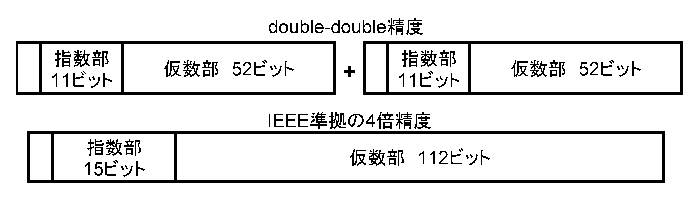
\includegraphics{double-double.eps}
\caption{double-double型のビット数}
\label{fig:residual}
  }
\end{figure}

\subsection{4倍精度演算の使用}
\label{sec:testprog4}
Toepliz行列
\[
A = \left(
\begin{array}{cccccc}
2 & 1 &   &  &  & \\
0 & 2 & 1 &  &  & \\
\gamma & 0& 2 & 1 &  & \\
 & \ddots & \ddots & \ddots & \ddots & \\
 &  &   \gamma &0 &       2   & 1 \\
 &  &  &   \gamma & 0& 2 \\
\end{array}
\right)
\]
に対する線型方程式$Ax=b$を指定された解法で解き, 解を標準出力に書き出す
検証プログラムが\verb|test5.c|である. 
右辺ベクトル$b$は解$x$がすべて$1$となるよう
設定される. $n$は行列$A$の次数である. 
\verb|test5|において, 
\newpage
{\bf 倍精度の場合}\\
\verb+      > ./test5 200 2.0 -f double+ \\
または \\
\verb+      > ./test5 200 2.0+ \\
と入力して実行すると, 以下の結果が得られる. 

\begin{verbatim}
n = 200, gamma = 2.000000

initial vector x      : all components set to 0
precision             : double
linear solver         : BiCG
preconditioner        : none
convergence condition : ||b-Ax||_2 <= 1.0e-12 * ||b-Ax_0||_2
matrix storage format : CSR
linear solver status  : normal end

BiCG: number of iterations = 1001 (double = 1001, quad = 0)
BiCG: elapsed time         = 2.044368e-02 sec.
BiCG:   preconditioner     = 4.768372e-06 sec.
BiCG:     matrix creation  = 4.768372e-06 sec.
BiCG:   linear solver      = 2.043891e-02 sec.
BiCG: relative residual    = 8.917591e+01
\end{verbatim}

{\bf 4倍精度の場合}\\
\verb+      > ./test5 200 2.0 -f quad+\\
と入力して実行すると, 以下の結果が得られる. 

\begin{verbatim}
n = 200, gamma = 2.000000

initial vector x      : all components set to 0
precision             : quad
linear solver         : BiCG
preconditioner        : none
convergence condition : ||b-Ax||_2 <= 1.0e-12 * ||b-Ax_0||_2
matrix storage format : CSR
linear solver status  : normal end

BiCG: number of iterations = 230 (double = 230, quad = 0)
BiCG: elapsed time         = 2.267408e-02 sec.
BiCG:   preconditioner     = 4.549026e-04 sec.
BiCG:     matrix creation  = 5.006790e-06 sec.
BiCG:   linear solver      = 2.221918e-02 sec.
BiCG: relative residual    = 6.499145e-11
\end{verbatim}

\newpage
\section{行列格納形式}
\label{sec:storages}
本節では, ライブラリで使用できる行列の格納形式について述べる. 
行列の行(列)番号は0から始まるものとする. 
次数$n \times n$の行列$A=(a_{ij})$の非零要素数を$nnz$とする. 

\subsection{Compressed Sparse Row (CSR)}
CSR形式では, データを3つの配列({\ttfamily ptr,index,value})に格納する. 
\begin{itemize}
\item 長さ$nnz$の倍精度配列{\ttfamily value}は, 行列$A$の非零要素の値を行方向に沿って格納する. 
\item 長さ$nnz$の整数配列{\ttfamily index}は, 配列{\ttfamily value}に格納された非零要素の列番号を格納する. 
\item 長さ$n+1$の整数配列{\ttfamily ptr}は, 配列{\ttfamily value}と{\ttfamily index}の各行の開始位置を格納する. 
\end{itemize}

\subsubsection{行列の作成 (逐次・マルチスレッド環境)}
行列$A$のCSR形式での格納方法を図\ref{fig:storage01}に示す. 
この行列をCSR形式で作成する場合, プログラムは以下のように記述する. 
\begin{figure}[h]
{\centering 
\begin{minipage}{0.3\textwidth}
\begin{flushright}
$ \label{eq:mata}
A = \left(
\begin{array}{cccc}
11 &    &    &    \\
21 & 22 &    &    \\
   & 32 & 33 &    \\
41 &    & 43 & 44 \\
\end{array}\right)
$
\end{flushright}
\end{minipage}
\begin{minipage}{0.6\textwidth}
\begin{flushleft}
\includegraphics{storage01.eps} 
\end{flushleft}
\end{minipage}
\caption{CSR形式のデータ構造 (逐次・マルチスレッド環境)}\label{fig:storage01}}
\end{figure}
\begin{itembox}[l]{逐次・マルチスレッド環境}
\small
\begin{verbatim}
 1: LIS_INT n,nnz;
 2: LIS_INT *ptr,*index;
 3: LIS_SCALAR *value;
 4: LIS_MATRIX A;
 5: n = 4; nnz = 8;
 6: ptr   = (LIS_INT *)malloc( (n+1)*sizeof(int) );
 7: index = (LIS_INT *)malloc( nnz*sizeof(int) );
 8: value = (LIS_SCALAR *)malloc( nnz*sizeof(LIS_SCALAR) );
 9: lis_matrix_create(0,&A);
10: lis_matrix_set_size(A,0,n);
11:
12: ptr[0] = 0; ptr[1] = 1; ptr[2] = 3; ptr[3] = 5; ptr[4] = 8;
13: index[0] =  0; index[1] =  0; index[2] =  1; index[3] =  1;
14: index[4] =  2; index[5] =  0; index[6] =  2; index[7] =  3;
15: value[0] = 11; value[1] = 21; value[2] = 22; value[3] = 32;
16: value[4] = 33; value[5] = 41; value[6] = 43; value[7] = 44;
17:
18: lis_matrix_set_csr(nnz,ptr,index,value,A);
19: lis_matrix_assemble(A);
\end{verbatim}
\end{itembox}

\subsubsection{行列の作成 (マルチプロセス環境)}
2プロセス上への行列$A$のCSR形式での格納方法を図\ref{fig:storage01_mpi}に示す. 
2プロセス上にこの行列をCSR形式で作成する場合, プログラムは以下のように記述する. 
\begin{figure}[h]
{\centering 
\includegraphics{storage01_mpi.eps} 
\caption{CSR形式のデータ構造 (マルチプロセス環境)}\label{fig:storage01_mpi}}
\end{figure}
\begin{itembox}[l]{マルチプロセス環境}
\small
\begin{verbatim}
 1: LIS_INT i,k,n,nnz,my_rank;
 2: LIS_INT *ptr,*index;
 3: LIS_SCALAR *value;
 4: LIS_MATRIX A;
 5: MPI_Comm_rank(MPI_COMM_WORLD,&my_rank);
 6: if( my_rank==0 ) {n = 2; nnz = 3;}
 7: else             {n = 2; nnz = 5;}
 8: ptr   = (LIS_INT *)malloc( (n+1)*sizeof(int) );
 9: index = (LIS_INT *)malloc( nnz*sizeof(int) );
10: value = (LIS_SCALAR *)malloc( nnz*sizeof(LIS_SCALAR) );
11: lis_matrix_create(MPI_COMM_WORLD,&A);
12: lis_matrix_set_size(A,n,0);
13: if( my_rank==0 ) {
14:     ptr[0] = 0; ptr[1] = 1; ptr[2] = 3;
15:     index[0] =  0; index[1] =  0; index[2] =  1;
16:     value[0] = 11; value[1] = 21; value[2] = 22;}
17: else {
18:     ptr[0] = 0; ptr[1] = 2; ptr[2] = 5;
19:     index[0] =  1; index[1] =  2; index[2] =  0; index[3] =  2; index[4] =  3;
20:     value[0] = 32; value[1] = 33; value[2] = 41; value[3] = 43; value[4] = 44;}
21: lis_matrix_set_csr(nnz,ptr,index,value,A);
22: lis_matrix_assemble(A);
\end{verbatim}
\end{itembox}

\subsubsection{関連する関数}
\noindent
{\bf 配列の関連付け}

CSR形式の配列を行列$A$に関連付けるには, 関数

\begin{itemize}
\item \verb|C       LIS_INT lis_matrix_set_csr(LIS_INT nnz, LIS_INT ptr[], LIS_INT index[],|\\
      \verb| LIS_SCALAR value[], LIS_MATRIX A)|
\item \verb|Fortran subroutine lis_matrix_set_csr(LIS_INTEGER nnz, LIS_INTEGER ptr(),|\\
      \verb| LIS_INTEGER index(), LIS_SCALAR value(), LIS_MATRIX A, LIS_INTEGER ierr)|
\end{itemize}

を用いる. 

\newpage
\subsection{Compressed Sparse Column (CSC)}
CSC形式では, データを3つの配列({\ttfamily ptr,index,value})に格納する. 
\begin{itemize}
\item 長さ$nnz$の倍精度配列{\ttfamily value}は, 行列$A$の非零要素の値を列方向に沿って格納する. 
\item 長さ$nnz$の整数配列{\ttfamily index}は, 配列{\ttfamily value}に格納された非零要素の行番号を格納する. 
\item 長さ$n+1$の整数配列{\ttfamily ptr}は, 配列{\ttfamily value}と{\ttfamily index}の各列の開始位置を格納する. 
\end{itemize}

\subsubsection{行列の作成 (逐次・マルチスレッド環境)}
行列$A$のCSC形式での格納方法を図\ref{fig:storage02}に示す. 
この行列をCSC形式で作成する場合, プログラムは以下のように記述する. 

\begin{figure}[h]
{\centering 
\begin{minipage}{0.3\textwidth}
\begin{flushright}
$ 
A = \left(
\begin{array}{cccc}
11 &    &    &    \\
21 & 22 &    &    \\
   & 32 & 33 &    \\
41 &    & 43 & 44 \\
\end{array}\right)
$
\end{flushright}
\end{minipage}
\begin{minipage}{0.6\textwidth}
\begin{flushleft}
\includegraphics{storage02.eps} 
\end{flushleft}
\end{minipage}
\caption{CSC形式のデータ構造 (逐次・マルチスレッド環境)}\label{fig:storage02}}
\end{figure}
\begin{itembox}[l]{逐次・マルチスレッド環境}
\small
\begin{verbatim}
 1: LIS_INT n,nnz;
 2: LIS_INT *ptr,*index;
 3: LIS_SCALAR *value;
 4: LIS_MATRIX A;
 5: n = 4; nnz = 8;
 6: ptr   = (LIS_INT *)malloc( (n+1)*sizeof(int) );
 7: index = (LIS_INT *)malloc( nnz*sizeof(int) );
 8: value = (LIS_SCALAR *)malloc( nnz*sizeof(LIS_SCALAR) );
 9: lis_matrix_create(0,&A);
10: lis_matrix_set_size(A,0,n);
11:
12: ptr[0] = 0; ptr[1] = 3; ptr[2] = 5; ptr[3] = 7; ptr[4] = 8;
13: index[0] =  0; index[1] =  1; index[2] =  3; index[3] =  1;
14: index[4] =  2; index[5] =  2; index[6] =  3; index[7] =  3;
15: value[0] = 11; value[1] = 21; value[2] = 41; value[3] = 22;
16: value[4] = 32; value[5] = 33; value[6] = 43; value[7] = 44;
17:
18: lis_matrix_set_csc(nnz,ptr,index,value,A);
19: lis_matrix_assemble(A);
\end{verbatim}
\end{itembox}

\newpage
\subsubsection{行列の作成 (マルチプロセス環境)}
2プロセス上への行列$A$のCSC形式での格納方法を図\ref{fig:storage02_mpi}に
示す. 
2プロセス上にこの行列をCSC形式で作成する場合, プログラムは以下のように記述する. 
\begin{figure}[h]
{\centering 
\includegraphics{storage02_mpi.eps} 
\caption{CSC形式のデータ構造 (マルチプロセス環境)}\label{fig:storage02_mpi}}
\end{figure}
\begin{itembox}[l]{マルチプロセス環境}
\small
\begin{verbatim}
 1: LIS_INT i,k,n,nnz,my_rank;
 2: LIS_INT *ptr,*index;
 3: LIS_SCALAR *value;
 4: LIS_MATRIX A;
 5: MPI_Comm_rank(MPI_COMM_WORLD,&my_rank);
 6: if( my_rank==0 ) {n = 2; nnz = 3;}
 7: else             {n = 2; nnz = 5;}
 8: ptr   = (LIS_INT *)malloc( (n+1)*sizeof(int) );
 9: index = (LIS_INT *)malloc( nnz*sizeof(int) );
10: value = (LIS_SCALAR *)malloc( nnz*sizeof(LIS_SCALAR) );
11: lis_matrix_create(MPI_COMM_WORLD,&A);
12: lis_matrix_set_size(A,n,0);
13: if( my_rank==0 ) {
14:     ptr[0] = 0; ptr[1] = 3; ptr[2] = 5;
15:     index[0] =  0; index[1] =  1; index[2] =  3; index[3] =  1; index[4] =  2;
16:     value[0] = 11; value[1] = 21; value[2] = 41; value[3] = 22; value[4] = 32}
17: else {
18:     ptr[0] = 0; ptr[1] = 2; ptr[2] = 3;
19:     index[0] =  2; index[1] =  3; index[2] =  3;
20:     value[0] = 33; value[1] = 43; value[2] = 44;}
21: lis_matrix_set_csc(nnz,ptr,index,value,A);
22: lis_matrix_assemble(A);
\end{verbatim}
\end{itembox}

\subsubsection{関連する関数}
\noindent
{\bf 配列の関連付け}

CSC形式の配列を行列$A$に関連付けるには, 関数
\begin{itemize}
\item \verb|C       LIS_INT lis_matrix_set_csc(LIS_INT nnz, LIS_INT ptr[], LIS_INT index[],|\\
      \verb| LIS_SCALAR value[], LIS_MATRIX A)|
\item \verb|Fortran subroutine lis_matrix_set_csc(LIS_INTEGER nnz, LIS_INTEGER ptr(),|\\
      \verb| LIS_INTEGER index(), LIS_SCALAR value(), LIS_MATRIX A, LIS_INTEGER ierr)|
\end{itemize}
を用いる. 

\newpage
\subsection{Modified Compressed Sparse Row (MSR)}
MSR形式では, データを2つの配列({\ttfamily index,value})に格納する. $ndz$を対角部分の零要素数とする. 
\begin{itemize}
\item 長さ$nnz + ndz + 1$の倍精度配列{\ttfamily value}は, 
第$n$要素までは行列$A$の対角部分を格納する. 第$n+1$要素は使用しない. 第
      $n+2$要素からは
行列$A$の対角部分以外の非零要素の値を行方向に沿って格納する. 
\item 長さ$nnz + ndz + 1$の整数配列{\ttfamily index}は, 
第$n+1$要素までは行列$A$の非対角部分の各行の開始位置を格納する. 
第$n+2$要素からは行列$A$の非対角部分の配列{\ttfamily value}に格納された非零要素の列番号を格納する. 
\end{itemize}

\subsubsection{行列の作成 (逐次・マルチスレッド環境)}
行列$A$のMSR形式での格納方法を図\ref{fig:storage03}に示す. 
この行列をMSR形式で作成する場合, プログラムは以下のように記述する. 

\begin{figure}[h]
{\centering 
\begin{minipage}{0.3\textwidth}
\begin{flushright}
$ 
A = \left(
\begin{array}{cccc}
11 &    &    &    \\
21 & 22 &    &    \\
   & 32 & 33 &    \\
41 &    & 43 & 44 \\
\end{array}\right)
$
\end{flushright}
\end{minipage}
\begin{minipage}{0.6\textwidth}
\begin{flushleft}
\includegraphics{storage03.eps} 
\end{flushleft}
\end{minipage}
\caption{MSR形式のデータ構造 (逐次・マルチスレッド環境)}\label{fig:storage03}}
\end{figure}
\begin{itembox}[l]{逐次・マルチスレッド環境}
\small
\begin{verbatim}
 1: LIS_INT n,nnz,ndz;
 2: LIS_INT *index;
 3: LIS_SCALAR *value;
 4: LIS_MATRIX A;
 5: n = 4; nnz = 8; ndz = 0;
 6: index = (LIS_INT *)malloc( (nnz+ndz+1)*sizeof(int) );
 7: value = (LIS_SCALAR *)malloc( (nnz+ndz+1)*sizeof(LIS_SCALAR) );
 8: lis_matrix_create(0,&A);
 9: lis_matrix_set_size(A,0,n);
10:
11: index[0] =  5; index[1] =  5; index[2] =  6; index[3] =  7;
12: index[4] =  9; index[5] =  0; index[6] =  1; index[7] =  0; index[8] =  2;
13: value[0] = 11; value[1] = 22; value[2] = 33; value[3] = 44;
14: value[4] =  0; value[5] = 21; value[6] = 32; value[7] = 41; value[8] = 43;
15:
16: lis_matrix_set_msr(nnz,ndz,index,value,A);
17: lis_matrix_assemble(A);
\end{verbatim}
\end{itembox}

\newpage
\subsubsection{行列の作成 (マルチプロセス環境)}
2プロセス上への行列$A$のMSR形式での格納方法を図\ref{fig:storage03_mpi}に
示す. 
2プロセス上にこの行列をMSR形式で作成する場合, プログラムは以下のように記述する. 
\begin{figure}[h]
{\centering 
\includegraphics{storage03_mpi.eps} 
\caption{MSR形式のデータ構造 (マルチプロセス環境)}\label{fig:storage03_mpi}}
\end{figure}
\begin{itembox}[l]{マルチプロセス環境}
\small
\begin{verbatim}
 1: LIS_INT i,k,n,nnz,ndz,my_rank;
 2: LIS_INT *index;
 3: LIS_SCALAR *value;
 4: LIS_MATRIX A;
 5: MPI_Comm_rank(MPI_COMM_WORLD,&my_rank);
 6: if( my_rank==0 ) {n = 2; nnz = 3; ndz = 0;}
 7: else             {n = 2; nnz = 5; ndz = 0;}
 8: index = (LIS_INT *)malloc( (nnz+ndz+1)*sizeof(int) );
 9: value = (LIS_SCALAR *)malloc( (nnz+ndz+1)*sizeof(LIS_SCALAR) );
10: lis_matrix_create(MPI_COMM_WORLD,&A);
11: lis_matrix_set_size(A,n,0);
12: if( my_rank==0 ) {
13:     index[0] =  3; index[1] =  3; index[2] =  4; index[3] =  0;
14:     value[0] = 11; value[1] = 22; value[2] =  0; value[3] = 21;}
15: else {
16:     index[0] =  3; index[1] =  4; index[2] =  6; index[3] =  1;
17:     index[4] =  0; index[5] =  2;
18:     value[0] = 33; value[1] = 44; value[2] =  0; value[3] = 32;
19:     value[4] = 41; value[5] = 43;}
20: lis_matrix_set_msr(nnz,ndz,index,value,A);
21: lis_matrix_assemble(A);
\end{verbatim}
\end{itembox}

\subsubsection{関連する関数}
\noindent
{\bf 配列の関連付け}

MSR形式の配列を行列$A$に関連付けるには, 関数
\begin{itemize}
\item \verb|C       LIS_INT lis_matrix_set_msr(LIS_INT nnz, LIS_INT ndz, LIS_INT index[],|\\
      \verb| LIS_SCALAR value[], LIS_MATRIX A)|
\item \verb|Fortran subroutine lis_matrix_set_msr(LIS_INTEGER nnz, LIS_INTEGER ndz,|\\
      \verb| LIS_INTEGER index(), LIS_SCALAR value(), LIS_MATRIX A, LIS_INTEGER ierr)|
\end{itemize}
を用いる. 

\newpage
\subsection{Diagonal (DIA)}
DIA形式では, データを2つの配列({\ttfamily index, value})に格納する. 
$nnd$を行列$A$の非零な対角要素の本数とする. 
\begin{itemize}
\item 長さ$nnd \times n$の倍精度配列{\ttfamily value}は, 行列$A$の非零な対
      角要素の値を格納する. 
\item 長さ$nnd$の整数配列{\ttfamily index}は, 主対角要素から各対角要素へのオフセットを格納する. 
\end{itemize}
マルチスレッド環境では以下のように格納する.\\
データを2つの配列({\ttfamily index, value})に格納する. $nprocs$をスレッド数とする. 
$nnd_p$を行列$A$を行ブロック分割した部分行列の非零な対角部分の本数とする. 
$maxnnd$を$nnd_p$の値の最大値とする. 
\begin{itemize}
\item 長さ$maxnnd \times n$の倍精度配列{\ttfamily value}は, 行列$A$を行ブ
      ロック分割した部分行列の非零な対角要素の値を格納する. 
\item 長さ$nprocs \times maxnnd$の整数配列{\ttfamily index}は, 主対角要素から各対角要素へのオフセットを格納する. 
\end{itemize}

\subsubsection{行列の作成 (逐次環境)}
行列$A$のDIA形式での格納方法を図\ref{fig:storage04}に示す. 
この行列をDIA形式で作成する場合, プログラムは以下のように記述する. 
\begin{figure}[h]
{\centering 
\begin{minipage}{0.3\textwidth}
\begin{flushright}
$ 
A = \left(
\begin{array}{cccc}
11 &    &    &    \\
21 & 22 &    &    \\
   & 32 & 33 &    \\
41 &    & 43 & 44 \\
\end{array}\right)
$
\end{flushright}
\end{minipage}
\begin{minipage}{0.6\textwidth}
\begin{flushleft}
\includegraphics{storage04.eps} 
\end{flushleft}
\end{minipage}
\caption{DIA形式のデータ構造 (逐次環境)}\label{fig:storage04}}
\end{figure}
\begin{itembox}[l]{逐次環境}
\small
\begin{verbatim}
 1: LIS_INT n,nnd;
 2: LIS_INT *index;
 3: LIS_SCALAR *value;
 4: LIS_MATRIX A;
 5: n = 4; nnd = 3;
 6: index = (LIS_INT *)malloc( nnd*sizeof(int) );
 7: value = (LIS_SCALAR *)malloc( n*nnd*sizeof(LIS_SCALAR) );
 8: lis_matrix_create(0,&A);
 9: lis_matrix_set_size(A,0,n);
10:
11: index[0] = -3; index[1] = -1; index[2] =  0;
12: value[0] =  0; value[1] =  0; value[2] =  0; value[3] = 41;
13: value[4] =  0; value[5] = 21; value[6] = 32; value[7] = 43;
14: value[8] = 11; value[9] = 22; value[10]= 33; value[11]= 44;
15:
16: lis_matrix_set_dia(nnd,index,value,A);
17: lis_matrix_assemble(A);
\end{verbatim}
\end{itembox}

\subsubsection{行列の作成 (マルチスレッド環境)}
2スレッド上への行列$A$のDIA形式での格納方法を図\ref{fig:storage04_omp}に
示す. 
2スレッド上にこの行列をDIA形式で作成する場合, プログラムは以下のように記述する. 
\begin{figure}[h]
{\centering 
\includegraphics{storage04_omp.eps} 
\caption{DIA形式のデータ構造 (マルチスレッド環境)}\label{fig:storage04_omp}}
\end{figure}
\begin{itembox}[l]{マルチスレッド環境}
\small
\begin{verbatim}
 1: LIS_INT n,maxnnd,nprocs;
 2: LIS_INT *index;
 3: LIS_SCALAR *value;
 4: LIS_MATRIX A;
 5: n = 4; maxnnd = 3; nprocs = 2;
 6: index = (LIS_INT *)malloc( maxnnd*sizeof(int) );
 7: value = (LIS_SCALAR *)malloc( n*maxnnd*sizeof(LIS_SCALAR) );
 8: lis_matrix_create(0,&A);
 9: lis_matrix_set_size(A,0,n);
10:
11: index[0] = -1; index[1] =  0; index[2] =  0; index[3] = -3; index[4] = -1; index[5] =  0;
12: value[0] =  0; value[1] = 21; value[2] = 11; value[3] = 22; value[4] =  0; value[5] =  0;
13: value[6] =  0; value[7] = 41; value[8] = 32; value[9] = 43; value[10]= 33; value[11]= 44;
14:
15: lis_matrix_set_dia(maxnnd,index,value,A);
16: lis_matrix_assemble(A);
\end{verbatim}
\end{itembox}
\newpage

\subsubsection{行列の作成 (マルチプロセス環境)}
2プロセス上への行列$A$のDIA形式での格納方法を図\ref{fig:storage04_mpi}に
示す. 
2プロセス上にこの行列をDIA形式で作成する場合, プログラムは以下のように記述する. 
\begin{figure}[h]
{\centering 
\includegraphics{storage04_mpi.eps} 
\caption{DIA形式のデータ構造 (マルチプロセス環境)}\label{fig:storage04_mpi}}
\end{figure}
\begin{itembox}[l]{マルチプロセス環境}
\small
\begin{verbatim}
 1: LIS_INT i,n,nnd,my_rank;
 2: LIS_INT *index;
 3: LIS_SCALAR *value;
 4: LIS_MATRIX A;
 5: MPI_Comm_rank(MPI_COMM_WORLD,&my_rank);
 6: if( my_rank==0 ) {n = 2; nnd = 2;}
 7: else             {n = 2; nnd = 3;}
 8: index = (LIS_INT *)malloc( nnd*sizeof(int) );
 9: value = (LIS_SCALAR *)malloc( n*nnd*sizeof(LIS_SCALAR) );
10: lis_matrix_create(MPI_COMM_WORLD,&A);
11: lis_matrix_set_size(A,n,0);
12: if( my_rank==0 ) {
13:     index[0] = -1; index[1] =  0;
14:     value[0] =  0; value[1] = 21; value[2] = 11; value[3] = 22;}
15: else {
16:     index[0] = -3; index[1] = -1; index[2] =  0;
17:     value[0] =  0; value[1] = 41; value[2] = 32; value[3] = 43; value[4] = 33;
18:     value[5] = 44;}
19: lis_matrix_set_dia(nnd,index,value,A);
20: lis_matrix_assemble(A);
\end{verbatim}
\end{itembox}

\subsubsection{関連する関数}
\noindent
{\bf 配列の関連付け}

DIA形式の配列を行列$A$に関連付けるには, 関数
\begin{itemize}
\item \verb|C       LIS_INT lis_matrix_set_dia(LIS_INT nnd, LIS_INT index[],|\\
      \verb| LIS_SCALAR value[], LIS_MATRIX A)|
\item \verb|Fortran subroutine lis_matrix_set_dia(LIS_INTEGER nnd, LIS_INTEGER index(),|\\
      \verb| LIS_SCALAR value(), LIS_MATRIX A, LIS_INTEGER ierr)|
\end{itemize}
を用いる. 

\newpage
\subsection{Ellpack-Itpack Generalized Diagonal (ELL)}
ELL形式では, データを2つの配列({\ttfamily index, value})に格納する. 
$maxnzr$を行列$A$の各行での非零要素数の最大値とする. 
\begin{itemize}
\item 長さ$maxnzr \times n$の倍精度配列{\ttfamily value}は, 行列$A$の各行の非零要素の値を列方向に沿って格納する. 
最初の列は各行の最初の非零要素からなる. ただし, 格納する非零要素がない場合は$0$を格納する. 
\item 長さ$maxnzr \times n$の整数配列{\ttfamily index}は, 
配列{\ttfamily value}に格納された非零要素の列番号を格納する. 
ただし, 第$i$行の非零要素数を$nnz$とすると{\tt index[$nnz \times n + i$]}にはその行番号$i$を格納する. 
\end{itemize}

\subsubsection{行列の作成 (逐次・マルチスレッド環境)}
行列$A$のELL形式での格納方法を図\ref{fig:storage05}に示す. 
この行列をELL形式で作成する場合, プログラムは以下のように記述する. 
\begin{figure}[h]
{\centering 
\begin{minipage}{0.3\textwidth}
\begin{flushright}
$ 
A = \left(
\begin{array}{cccc}
11 &    &    &    \\
21 & 22 &    &    \\
   & 32 & 33 &    \\
41 &    & 43 & 44 \\
\end{array}\right)
$
\end{flushright}
\end{minipage}
\begin{minipage}{0.6\textwidth}
\begin{flushleft}
\includegraphics{storage05.eps} 
\end{flushleft}
\end{minipage}
\caption{ELL形式のデータ構造 (逐次・マルチスレッド環境)}\label{fig:storage05}}
\end{figure}
\begin{itembox}[l]{逐次・マルチスレッド環境}
\small
\begin{verbatim}
 1: LIS_INT n,maxnzr;
 2: LIS_INT *index;
 3: LIS_SCALAR *value;
 4: LIS_MATRIX A;
 5: n = 4; maxnzr = 3;
 6: index = (LIS_INT *)malloc( n*maxnzr*sizeof(int) );
 7: value = (LIS_SCALAR *)malloc( n*maxnzr*sizeof(LIS_SCALAR) );
 8: lis_matrix_create(0,&A);
 9: lis_matrix_set_size(A,0,n);
10:
11: index[0] =  0; index[1] =  0; index[2] =  1; index[3] =  0; index[4] =  0; index[5] =  1;
12: index[6] =  2; index[7] =  2; index[8] =  0; index[9] =  1; index[10]=  2; index[11]=  3;
13: value[0] = 11; value[1] = 21; value[2] = 32; value[3] = 41; value[4] =  0; value[5] = 22;
14: value[6] = 33; value[7] = 43; value[8] =  0; value[9] =  0; value[10]=  0; value[11]= 44;
15:
16: lis_matrix_set_ell(maxnzr,index,value,A);
17: lis_matrix_assemble(A);
\end{verbatim}
\end{itembox}

\newpage
\subsubsection{行列の作成 (マルチプロセス環境)}
2プロセス上への行列$A$のELL形式での格納方法を図\ref{fig:storage05_mpi}に
示す. 
2プロセス上にこの行列をELL形式で作成する場合, プログラムは以下のように記述する. 
\begin{figure}[h]
{\centering 
\includegraphics{storage05_mpi.eps} 
\caption{ELL形式のデータ構造 (マルチプロセス環境)}\label{fig:storage05_mpi}}
\end{figure}
\begin{itembox}[l]{マルチプロセス環境}
\small
\begin{verbatim}
 1: LIS_INT i,n,maxnzr,my_rank;
 2: LIS_INT *index;
 3: LIS_SCALAR *value;
 4: LIS_MATRIX A;
 5: MPI_Comm_rank(MPI_COMM_WORLD,&my_rank);
 6: if( my_rank==0 ) {n = 2; maxnzr = 2;}
 7: else             {n = 2; maxnzr = 3;}
 8: index = (LIS_INT *)malloc( n*maxnzr*sizeof(int) );
 9: value = (LIS_SCALAR *)malloc( n*maxnzr*sizeof(LIS_SCALAR) );
10: lis_matrix_create(MPI_COMM_WORLD,&A);
11: lis_matrix_set_size(A,n,0);
12: if( my_rank==0 ) {
13:     index[0] =  0; index[1] =  0; index[2] =  0; index[3] =  1;
14:     value[0] = 11; value[1] = 21; value[2] =  0; value[3] = 22;}
15: else {
16:     index[0] =  1; index[1] =  0; index[2] =  2; index[3] =  2; index[4] =  2;
17:     index[5] =  3;
18:     value[0] = 32; value[1] = 41; value[2] = 33; value[3] = 43; value[4] =  0;
19:     value[5] = 44;}
20: lis_matrix_set_ell(maxnzr,index,value,A);
21: lis_matrix_assemble(A);
\end{verbatim}
\end{itembox}

\subsubsection{関連する関数}
\noindent
{\bf 配列の関連付け}

ELL形式の配列を行列$A$に関連付けるには, 関数
\begin{itemize}
\item \verb|C       LIS_INT lis_matrix_set_ell(LIS_INT maxnzr, LIS_INT index[],|\\
      \verb| LIS_SCALAR value[], LIS_MATRIX A)|
\item \verb|Fortran subroutine lis_matrix_set_ell(LIS_INTEGER maxnzr, LIS_INTEGER index(),|\\
      \verb| LIS_SCALAR value(), LIS_MATRIX A, LIS_INTEGER ierr)|
\end{itemize}
を用いる. 

\newpage
\subsection{Jagged Diagonal (JAD)}
JAD形式では, 最初に各行の非零要素数の大きい順に行の並び替えを行い, 
各行の非零要素を列方向に沿って格納する. 
JAD形式では, データを4つの配列({\ttfamily perm, ptr, index, value})に格納する. 
$maxnzr$を行列$A$の各行での非零要素数の最大値とする. 
\begin{itemize}
\item 長さ$n$の整数配列{\ttfamily perm}は, 並び替えた行番号を格納する. 
\item 長さ$nnz$の倍精度配列{\ttfamily value}は, 並び替えられた行列$A$の鋸
      歯状対角要素の値を格納する. 
最初の鋸歯状対角要素は各行の第1非零要素からなる. 
次の鋸歯状対角要素は各行の第2非零要素からなる. これを順次繰り返していく. 
\item 長さ$nnz$の整数配列{\ttfamily index}は, 配列{\ttfamily value}に格納された非零要素の列番号を格納する. 
\item 長さ$maxnzr + 1$の整数配列{\ttfamily ptr}は, 各鋸歯状対角要素の開始位置を格納する. 
\end{itemize}
マルチスレッド環境では以下のように格納する.\\
データを4つの配列({\ttfamily perm, ptr, index, value})に格納する. 
$nprocs$をスレッド数とする. 
$maxnzr_p$を行列$A$を行ブロック分割した部分行列の各行での非零要素数の最大値とする. 
$maxmaxnzr$は配列$maxnzr_p$の値の最大値である. 
\begin{itemize}
\item 長さ$n$の整数配列{\ttfamily perm}は, 行列$A$を行ブロック分割した部分行列を並び替えた行番号を格納する. 
\item 長さ$nnz$の倍精度配列{\ttfamily value}は, 並び替えられた行列$A$の鋸
      歯状対角要素の値を格納する. 
最初の鋸歯状対角要素は各行の第1非零要素からなる. 
次の鋸歯状対角要素は各行の第2非零要素からなる. これを順次繰り返していく. 
\item 長さ$nnz$の整数配列{\ttfamily index}は, 配列{\ttfamily value}に格納された非零要素の列番号を格納する. 
\item 長さ$nprocs \times (maxmaxnzr + 1)$の整数配列{\ttfamily ptr}は, 行列
      $A$を行ブロック分割した部分行列の各鋸歯状対角要素の開始位置を格納する. 
\end{itemize}

\newpage
\subsubsection{行列の作成 (逐次環境)}
行列$A$のJAD形式での格納方法を図\ref{fig:storage06}に示す. 
この行列をJAD形式で作成する場合, プログラムは以下のように記述する. 
\begin{figure}[h]
{\centering 
\begin{minipage}{0.3\textwidth}
\begin{flushright}
$ 
A = \left(
\begin{array}{cccc}
11 &    &    &    \\
21 & 22 &    &    \\
   & 32 & 33 &    \\
41 &    & 43 & 44 \\
\end{array}\right)
$
\end{flushright}
\end{minipage}
\begin{minipage}{0.6\textwidth}
\begin{flushleft}
\includegraphics{storage06.eps} 
\end{flushleft}
\end{minipage}
\caption{JAD形式のデータ構造 (逐次環境)}\label{fig:storage06}}
\end{figure}
\begin{itembox}[l]{逐次環境}
\small
\begin{verbatim}
 1: LIS_INT n,nnz,maxnzr;
 2: LIS_INT *perm,*ptr,*index;
 3: LIS_SCALAR *value;
 4: LIS_MATRIX A;
 5: n = 4; nnz = 8; maxnzr = 3;
 6: perm  = (LIS_INT *)malloc( n*sizeof(int) );
 7: ptr   = (LIS_INT *)malloc( (maxnzr+1)*sizeof(int) );
 8: index = (LIS_INT *)malloc( nnz*sizeof(int) );
 9: value = (LIS_SCALAR *)malloc( nnz*sizeof(LIS_SCALAR) );
10: lis_matrix_create(0,&A);
11: lis_matrix_set_size(A,0,n);
12:
13: perm[0] = 3; perm[1] = 1; perm[2] = 2; perm[3] = 0;
14: ptr[0]  = 0; ptr[1]  = 4; ptr[2]  = 7; ptr[3]  = 8;
15: index[0] =  0; index[1] =  0; index[2] =  1; index[3] =  0;
16: index[4] =  2; index[5] =  1; index[6] =  2; index[7] =  3;
17: value[0] = 41; value[1] = 21; value[2] = 32; value[3] = 11;
18: value[4] = 43; value[5] = 22; value[6] = 33; value[7] = 44;
19:
20: lis_matrix_set_jad(nnz,maxnzr,perm,ptr,index,value,A);
21: lis_matrix_assemble(A);
\end{verbatim}
\end{itembox}

\newpage
\subsubsection{行列の作成 (マルチスレッド環境)}
2スレッド上への行列$A$のJAD形式での格納方法を図\ref{fig:storage06_omp}に
示す. 
2スレッド上にこの行列をJAD形式で作成する場合, プログラムは以下のように記述する. 
\begin{figure}[h]
{\centering 
\includegraphics{storage06_omp.eps} 
\caption{JAD形式のデータ構造 (マルチスレッド環境)}\label{fig:storage06_omp}}
\end{figure}
\begin{itembox}[l]{マルチスレッド環境}
\small
\begin{verbatim}
 1: LIS_INT n,nnz,maxmaxnzr,nprocs;
 2: LIS_INT *perm,*ptr,*index;
 3: LIS_SCALAR *value;
 4: LIS_MATRIX A;
 5: n = 4; nnz = 8; maxmaxnzr = 3; nprocs = 2;
 6: perm  = (LIS_INT *)malloc( n*sizeof(int) );
 7: ptr   = (LIS_INT *)malloc( nprocs*(maxmaxnzr+1)*sizeof(int) );
 8: index = (LIS_INT *)malloc( nnz*sizeof(int) );
 9: value = (LIS_SCALAR *)malloc( nnz*sizeof(LIS_SCALAR) );
10: lis_matrix_create(0,&A);
11: lis_matrix_set_size(A,0,n);
12:
13: perm[0] = 1; perm[1] = 0; perm[2] = 3; perm[3] = 2;
14: ptr[0]  = 0; ptr[1]  = 2; ptr[2]  = 3; ptr[3]  = 0;
15: ptr[4]  = 3; ptr[5]  = 5; ptr[6]  = 7; ptr[7]  = 8;
16: index[0] =  0; index[1] =  0; index[2] =  1; index[3] =  0;
17: index[4] =  1; index[5] =  2; index[6] =  2; index[7] =  3;
18: value[0] = 21; value[1] = 11; value[2] = 22; value[3] = 41;
19: value[4] = 32; value[5] = 43; value[6] = 33; value[7] = 44;
20:
21: lis_matrix_set_jad(nnz,maxmaxnzr,perm,ptr,index,value,A);
22: lis_matrix_assemble(A);
\end{verbatim}
\end{itembox}

\newpage
\subsubsection{行列の作成 (マルチプロセス環境)}
2プロセス上への行列$A$のJAD形式での格納方法を図\ref{fig:storage06_mpi}に
示す. 
2プロセス上にこの行列をJAD形式で作成する場合, プログラムは以下のように記述する. 
\begin{figure}[h]
{\centering 
\includegraphics{storage06_mpi.eps} 
\caption{JAD形式のデータ構造 (マルチプロセス環境)}\label{fig:storage06_mpi}}
\end{figure}
\begin{itembox}[l]{マルチプロセス環境}
\small
\begin{verbatim}
 1: LIS_INT i,n,nnz,maxnzr,my_rank;
 2: LIS_INT *perm,*ptr,*index;
 3: LIS_SCALAR *value;
 4: LIS_MATRIX A;
 5: MPI_Comm_rank(MPI_COMM_WORLD,&my_rank);
 6: if( my_rank==0 ) {n = 2; nnz = 3; maxnzr = 2;}
 7: else             {n = 2; nnz = 5; maxnzr = 3;}
 8: perm  = (LIS_INT *)malloc( n*sizeof(int) );
 9: ptr   = (LIS_INT *)malloc( (maxnzr+1)*sizeof(int) );
10: index = (LIS_INT *)malloc( nnz*sizeof(int) );
11: value = (LIS_SCALAR *)malloc( nnz*sizeof(LIS_SCALAR) );
12: lis_matrix_create(MPI_COMM_WORLD,&A);
13: lis_matrix_set_size(A,n,0);
14: if( my_rank==0 ) {
15:     perm[0] = 1; perm[1] = 0;
16:     ptr[0]  = 0; ptr[1]  = 2; ptr[2]  = 3;
17:     index[0] =  0; index[1] =  0; index[2] =  1;
18:     value[0] = 21; value[1] = 11; value[2] = 22;}
19: else {
20:     perm[0] = 3; perm[1] = 2;
21:     ptr[0]  = 0; ptr[1]  = 2; ptr[2]  = 4; ptr[3]  = 5;
22:     index[0] =  0; index[1] =  1; index[2] =  2; index[3] =  2; index[4] =  3;
23:     value[0] = 41; value[1] = 32; value[2] = 43; value[3] = 33; value[4] = 44;}
24: lis_matrix_set_jad(nnz,maxnzr,perm,ptr,index,value,A);
25: lis_matrix_assemble(A);
\end{verbatim}
\end{itembox}

\subsubsection{関連する関数}
\noindent
{\bf 配列の関連付け}

JAD形式の配列を行列$A$に関連付けるには, 関数
\begin{itemize}
\item \verb|C       LIS_INT lis_matrix_set_jad(LIS_INT nnz, LIS_INT maxnzr, LIS_INT perm[],|\\
      \verb| LIS_INT ptr[], LIS_INT index[], LIS_SCALAR value[], LIS_MATRIX A)|
\item \verb|Fortran subroutine lis_matrix_set_jad(LIS_INTEGER nnz, LIS_INTEGER maxnzr,|\\
      \verb| LIS_INTEGER perm(), LIS_INTEGER ptr(), LIS_INTEGER index(), LIS_SCALAR value(),|\\
      \verb| LIS_MATRIX A, LIS_INTEGER ierr)|
\end{itemize}
を用いる. 

\newpage
\subsection{Block Sparse Row (BSR)}
BSR形式では, 行列を$r \times c$の大きさの部分行列 (ブロックと呼ぶ) に分解する. 
BSR形式では, CSR形式と同様の手順で非零ブロック (少なくとも1つの
非零要素が存在する) を格納する. 
$nr=n/r$, $bnnz$を$A$の非零ブロック数とする. 
BSR形式では, データを3つの配列({\ttfamily bptr, bindex, value})に格納する. 
\begin{itemize}
\item 長さ$bnnz \times r \times c$の倍精度配列{\ttfamily value}は, 非零ブロックの全要素の値を格納する. 
\item 長さ$bnnz$の整数配列{\ttfamily bindex}は, 非零ブロックのブロック列番号を格納する. 
\item 長さ$nr+1$の整数配列{\ttfamily bptr}は, 配列{\ttfamily bindex}のブロック行の開始位置を格納する. 
\end{itemize}

\subsubsection{行列の作成 (逐次・マルチスレッド環境)}
行列$A$のBSR形式での格納方法を図\ref{fig:storage07}に示す. 
この行列をBSR形式で作成する場合, プログラムは以下のように記述する. 
\begin{figure}[h]
{\centering 
\begin{minipage}{0.3\textwidth}
\begin{flushright}
$ 
A = \left(
\begin{array}{cc|cc}
11 &    &    &    \\
21 & 22 &    &    \\ \hline
   & 32 & 33 &    \\
41 &    & 43 & 44 \\
\end{array}\right)
$
\end{flushright}
\end{minipage}
\begin{minipage}{0.6\textwidth}
\begin{flushleft}
\includegraphics{storage07.eps} 
\end{flushleft}
\end{minipage}
\caption{BSR形式のデータ構造 (逐次・マルチスレッド環境)}\label{fig:storage07}}
\end{figure}
\begin{itembox}[l]{逐次・マルチスレッド環境}
\small
\begin{verbatim}
 1: LIS_INT n,bnr,bnc,nr,nc,bnnz;
 2: LIS_INT *bptr,*bindex;
 3: LIS_SCALAR *value;
 4: LIS_MATRIX A;
 5: n = 4; bnr = 2; bnc = 2; bnnz = 3; nr = (n-1)/bnr+1; nc = (n-1)/bnc+1;
 6: bptr   = (LIS_INT *)malloc( (nr+1)*sizeof(int) );
 7: bindex = (LIS_INT *)malloc( bnnz*sizeof(int) );
 8: value  = (LIS_SCALAR *)malloc( bnr*bnc*bnnz*sizeof(LIS_SCALAR) );
 9: lis_matrix_create(0,&A);
10: lis_matrix_set_size(A,0,n);
11:
12: bptr[0] = 0; bptr[1] = 1; bptr[2] = 3;
13: bindex[0] =  0; bindex[1] =  0; bindex[2] =  1;
14: value[0]  = 11; value[1] = 21; value[2] =  0; value[3] = 22;
15: value[4]  =  0; value[5] = 41; value[6] = 32; value[7] =  0;
16: value[8]  = 33; value[9] = 43; value[10]=  0; value[11]= 44;
17:
18: lis_matrix_set_bsr(bnr,bnc,bnnz,bptr,bindex,value,A);
19: lis_matrix_assemble(A);
\end{verbatim}
\end{itembox}

\newpage
\subsubsection{行列の作成 (マルチプロセス環境)}
2プロセス上への行列$A$のBSR形式での格納方法を図\ref{fig:storage07_mpi}に
示す. 
2プロセス上にこの行列をBSR形式で作成する場合, プログラムは以下のように記述する. 
\begin{figure}[h]
{\centering 
\includegraphics{storage07_mpi.eps} 
\caption{BSR形式のデータ構造 (マルチプロセス環境)}\label{fig:storage07_mpi}}
\end{figure}
\begin{itembox}[l]{マルチプロセス環境}
\small
\begin{verbatim}
 1: LIS_INT n,bnr,bnc,nr,nc,bnnz,my_rank;
 2: LIS_INT *bptr,*bindex;
 3: LIS_SCALAR *value;
 4: LIS_MATRIX A;
 5: MPI_Comm_rank(MPI_COMM_WORLD,&my_rank);
 6: if( my_rank==0 ) {n = 2; bnr = 2; bnc = 2; bnnz = 1; nr = (n-1)/bnr+1; nc = (n-1)/bnc+1;}
 7: else             {n = 2; bnr = 2; bnc = 2; bnnz = 2; nr = (n-1)/bnr+1; nc = (n-1)/bnc+1;}
 8: bptr   = (LIS_INT *)malloc( (nr+1)*sizeof(int) );
 9: bindex = (LIS_INT *)malloc( bnnz*sizeof(int) );
10: value  = (LIS_SCALAR *)malloc( bnr*bnc*bnnz*sizeof(LIS_SCALAR) );
11: lis_matrix_create(MPI_COMM_WORLD,&A);
12: lis_matrix_set_size(A,n,0);
13: if( my_rank==0 ) {
14:     bptr[0] = 0; bptr[1] = 1;
15:     bindex[0] =  0;
16:     value[0]  = 11; value[1] = 21; value[2] =  0; value[3] = 22;}
17: else {
18:     bptr[0] = 0; bptr[1] = 2;
19:     bindex[0] =  0; bindex[1] =  1;
20:     value[0]  =  0; value[1]  = 41; value[2] = 32; value[3] =  0;
21:     value[4]  = 33; value[5]  = 43; value[6] =  0; value[7] = 44;}
22: lis_matrix_set_bsr(bnr,bnc,bnnz,bptr,bindex,value,A);
23: lis_matrix_assemble(A);
\end{verbatim}
\end{itembox}

\subsubsection{関連する関数}
\noindent
{\bf 配列の関連付け}

BSR形式の配列を行列$A$に関連付けるには, 関数
\begin{itemize}
\item \verb|C       LIS_INT lis_matrix_set_bsr(LIS_INT bnr, LIS_INT bnc, LIS_INT bnnz,|\\
      \verb| LIS_INT bptr[], LIS_INT bindex[], LIS_SCALAR value[], LIS_MATRIX A)|
\item \verb|Fortran subroutine lis_matrix_set_bsr(LIS_INTEGER bnr, LIS_INTEGER bnc,|\\
      \verb| LIS_INTEGER bnnz, LIS_INTEGER bptr(), LIS_INTEGER bindex(), LIS_SCALAR value(),|\\
      \verb| LIS_MATRIX A, LIS_INTEGER ierr)|
\end{itemize}
を用いる. 

\subsection{Block Sparse Column (BSC)}
BSC形式では, 行列を$r \times c$の大きさの部分行列 (ブロックと呼ぶ) に分解する. 
BSC形式では, CSC形式と同様の手順で非零ブロック (少なくとも1つの
非零要素が存在する) を格納する. 
$nc=n/c$, $bnnz$を$A$の非零ブロック数とする. 
BSC形式では, データを3つの配列({\ttfamily bptr, bindex, value})に格納する. 
\begin{itemize}
\item 長さ$bnnz \times r \times c$の倍精度配列{\ttfamily value}は, 非零ブロックの全要素の値を格納する. 
\item 長さ$bnnz$の整数配列{\ttfamily bindex}は, 非零ブロックのブロック行番号を格納する. 
\item 長さ$nc+1$の整数配列{\ttfamily bptr}は, 配列{\ttfamily bindex}のブロック列の開始位置を格納する. 
\end{itemize}

\subsubsection{行列の作成 (逐次・マルチスレッド環境)}
行列$A$のBSC形式での格納方法を図\ref{fig:storage08}に示す. 
この行列をBSC形式で作成する場合, プログラムは以下のように記述する. 
\begin{figure}[h]
{\centering 
\begin{minipage}{0.3\textwidth}
\begin{flushright}
$ 
A = \left(
\begin{array}{cc|cc}
11 &    &    &    \\
21 & 22 &    &    \\ \hline
   & 32 & 33 &    \\
41 &    & 43 & 44 \\
\end{array}\right)
$
\end{flushright}
\end{minipage}
\begin{minipage}{0.6\textwidth}
\begin{flushleft}
\includegraphics{storage08.eps} 
\end{flushleft}
\end{minipage}
\caption{BSC形式のデータ構造 (逐次・マルチスレッド環境)}\label{fig:storage08}}
\end{figure}
\begin{itembox}[l]{逐次・マルチスレッド環境}
\small
\begin{verbatim}
 1: LIS_INT n,bnr,bnc,nr,nc,bnnz;
 2: LIS_INT *bptr,*bindex;
 3: LIS_SCALAR *value;
 4: LIS_MATRIX A;
 5: n = 4; bnr = 2; bnc = 2; bnnz = 3; nr = (n-1)/bnr+1; nc = (n-1)/bnc+1;
 6: bptr   = (LIS_INT *)malloc( (nc+1)*sizeof(int) );
 7: bindex = (LIS_INT *)malloc( bnnz*sizeof(int) );
 8: value  = (LIS_SCALAR *)malloc( bnr*bnc*bnnz*sizeof(LIS_SCALAR) );
 9: lis_matrix_create(0,&A);
10: lis_matrix_set_size(A,0,n);
11:
12: bptr[0] = 0; bptr[1] = 1; bptr[2] = 3;
13: bindex[0] =  0; bindex[1] =  1; bindex[2] =  1;
14: value[0]  = 11; value[1] = 21; value[2] =  0; value[3] = 22;
15: value[4]  =  0; value[5] = 41; value[6] = 32; value[7] =  0;
16: value[8]  = 33; value[9] = 43; value[10]=  0; value[11]= 44;
17:
18: lis_matrix_set_bsc(bnr,bnc,bnnz,bptr,bindex,value,A);
19: lis_matrix_assemble(A);
\end{verbatim}
\end{itembox}

\newpage
\subsubsection{行列の作成 (マルチプロセス環境)}
2プロセス上への行列$A$のBSC形式での格納方法を図\ref{fig:storage08_mpi}に
示す. 
2プロセス上にこの行列をBSC形式で作成する場合, プログラムは以下のように記述する. 
\begin{figure}[h]
{\centering 
\includegraphics{storage08_mpi.eps} 
\caption{BSC形式のデータ構造 (マルチプロセス環境)}\label{fig:storage08_mpi}}
\end{figure}
\begin{itembox}[l]{マルチプロセス環境}
\small
\begin{verbatim}
 1: LIS_INT n,bnr,bnc,nr,nc,bnnz,my_rank;
 2: LIS_INT *bptr,*bindex;
 3: LIS_SCALAR *value;
 4: LIS_MATRIX A;
 5: MPI_Comm_rank(MPI_COMM_WORLD,&my_rank);
 6: if( my_rank==0 ) {n = 2; bnr = 2; bnc = 2; bnnz = 2; nr = (n-1)/bnr+1; nc = (n-1)/bnc+1;}
 7: else             {n = 2; bnr = 2; bnc = 2; bnnz = 1; nr = (n-1)/bnr+1; nc = (n-1)/bnc+1;}
 8: bptr   = (LIS_INT *)malloc( (nr+1)*sizeof(int) );
 9: bindex = (LIS_INT *)malloc( bnnz*sizeof(int) );
10: value  = (LIS_SCALAR *)malloc( bnr*bnc*bnnz*sizeof(LIS_SCALAR) );
11: lis_matrix_create(MPI_COMM_WORLD,&A);
12: lis_matrix_set_size(A,n,0);
13: if( my_rank==0 ) {
14:     bptr[0] = 0; bptr[1] = 2;
15:     bindex[0] =  0; bindex[1] =  1;
16:     value[0]  = 11; value[1]  = 21; value[2] =  0; value[3] = 22;
17:     value[4]  =  0; value[5]  = 41; value[6] = 32; value[7] =  0;}
18: else {
19:     bptr[0] = 0; bptr[1] = 1;
20:     bindex[0] =  1;
21:     value[0]  = 33; value[1]  = 43; value[2] =  0; value[3] = 44;}
22: lis_matrix_set_bsc(bnr,bnc,bnnz,bptr,bindex,value,A);
23: lis_matrix_assemble(A);
\end{verbatim}
\end{itembox}

\subsubsection{関連する関数}
\noindent
{\bf 配列の関連付け}

BSC形式の配列を行列$A$に関連付けるには, 関数
\begin{itemize}
\item \verb|C       LIS_INT lis_matrix_set_bsc(LIS_INT bnr, LIS_INT bnc, LIS_INT bnnz,|\\
      \verb| LIS_INT bptr[], LIS_INT bindex[], LIS_SCALAR value[], LIS_MATRIX A)|
\item \verb|Fortran subroutine lis_matrix_set_bsc(LIS_INTEGER bnr, LIS_INTEGER bnc,|\\
      \verb| LIS_INTEGER bnnz, LIS_INTEGER bptr(), LIS_INTEGER bindex(), LIS_SCALAR value(),|\\
      \verb| LIS_MATRIX A, LIS_INTEGER ierr)|
\end{itemize}
を用いる. 

\newpage
\subsection{Variable Block Row (VBR)}
VBR形式はBSR形式を一般化したものである. 
行と列の分割位置は配列({\ttfamily row, col})で与えられる. 
VBR形式では, CSR形式と同様の手順で非零ブロック (少なくとも1つの
非零要素が存在する) を格納する. 
$nr$, $nc$をそれぞれ行分割数, 列分割数とする. 
$bnnz$を$A$の非零ブロック数, $nnz$を非零ブロックの全要素数とする. 
VBR形式では, データを6つの配列({\ttfamily bptr, bindex, row, col, ptr, value})に格納する. 
\begin{itemize}
\item 長さ$nr+1$の整数配列{\ttfamily row}は, ブロック行の開始行番号を格納する. 
\item 長さ$nc+1$の整数配列{\ttfamily col}は, ブロック列の開始列番号を格納する. 
\item 長さ$bnnz$の整数配列{\ttfamily bindex}は, 非零ブロックのブロック列番号を格納する. 
\item 長さ$nr+1$の整数配列{\ttfamily bptr}は, 配列{\ttfamily bindex}のブロック行の開始位置を格納する. 
\item 長さ$nnz$の倍精度配列{\ttfamily value}は, 非零ブロックの全要素の値を格納する. 
\item 長さ$bnnz+1$の整数配列{\ttfamily ptr}は, 配列{\ttfamily value}の非
      零ブロックの開始位置を格納する. 

\newpage
\subsubsection{行列の作成 (逐次・マルチスレッド環境)}
行列$A$のVBR形式での格納方法を図\ref{fig:storage09}に示す. 
この行列をVBR形式で作成する場合, プログラムは以下のように記述する. 
\end{itemize}
\begin{figure}[h]
{\centering 
\begin{minipage}{0.3\textwidth}
\begin{flushright}
$ 
A = \left(
\begin{array}{c|cc|c}
11 &    &    &    \\ \hline
21 & 22 &    &    \\
   & 32 & 33 &    \\ \hline
41 &    & 43 & 44 \\
\end{array}\right)
$
\end{flushright}
\end{minipage}
\begin{minipage}{0.6\textwidth}
\begin{flushleft}
\includegraphics{storage09.eps} 
\end{flushleft}
\end{minipage}
\caption{VBR形式のデータ構造 (逐次・マルチスレッド環境)}\label{fig:storage09}}
\end{figure}
\begin{itembox}[l]{逐次・マルチスレッド環境}
\small
\begin{verbatim}
 1: LIS_INT n,nnz,nr,nc,bnnz;
 2: LIS_INT *row,*col,*ptr,*bptr,*bindex;
 3: LIS_SCALAR *value;
 4: LIS_MATRIX A;
 5: n = 4; nnz = 11; bnnz = 6; nr = 3; nc = 3;
 6: bptr   = (LIS_INT *)malloc( (nr+1)*sizeof(int) );
 7: row    = (LIS_INT *)malloc( (nr+1)*sizeof(int) );
 8: col    = (LIS_INT *)malloc( (nc+1)*sizeof(int) );
 9: ptr    = (LIS_INT *)malloc( (bnnz+1)*sizeof(int) );
10: bindex = (LIS_INT *)malloc( bnnz*sizeof(int) );
11: value  = (LIS_SCALAR *)malloc( nnz*sizeof(LIS_SCALAR) );
12: lis_matrix_create(0,&A);
13: lis_matrix_set_size(A,0,n);
14:
15: bptr[0] = 0; bptr[1] = 1; bptr[2] = 3; bptr[3] = 6;
16: row[0]  = 0; row[1]  = 1; row[2]  = 3; row[3] = 4;
17: col[0]  = 0; col[1]  = 1; col[2]  = 3; col[3] = 4;
18: bindex[0] =  0; bindex[1] =  0; bindex[2] =  1; bindex[3] =  0;
19: bindex[4] =  1; bindex[5] =  2;
20: ptr[0]    =  0; ptr[1]    =  1; ptr[2]    =  3; ptr[3]    =  7;
21: ptr[4]    =  8; ptr[5]    = 10; ptr[6]    = 11;
22: value[0]  = 11; value[1]  = 21; value[2]  =  0; value[3]  = 22;
23: value[4]  = 32; value[5]  =  0; value[6]  = 33; value[7]  = 41;
24: value[8]  =  0; value[9]  = 43; value[10] = 44;
25:
26: lis_matrix_set_vbr(nnz,nr,nc,bnnz,row,col,ptr,bptr,bindex,value,A);
27: lis_matrix_assemble(A);
\end{verbatim}
\end{itembox}

\newpage
\subsubsection{行列の作成 (マルチプロセス環境)}
2プロセス上への行列$A$のVBR形式での格納方法を図\ref{fig:storage09_mpi}に
示す. 
2プロセス上にこの行列をVBR形式で作成する場合, プログラムは以下のように記述する. 
\begin{figure}[h]
{\centering 
\includegraphics{storage09_mpi.eps} 
\caption{VBR形式のデータ構造 (逐次・マルチスレッド環境)}\label{fig:storage09_mpi}}
\end{figure}
\begin{itembox}[l]{マルチプロセス環境}
\small
\begin{verbatim}
 1: LIS_INT n,nnz,nr,nc,bnnz,my_rank;
 2: LIS_INT *row,*col,*ptr,*bptr,*bindex;
 3: LIS_SCALAR *value;
 4: LIS_MATRIX A;
 5: MPI_Comm_rank(MPI_COMM_WORLD,&my_rank);
 6: if( my_rank==0 ) {n = 2; nnz = 7; bnnz = 3; nr = 2; nc = 3;}
 7: else             {n = 2; nnz = 4; bnnz = 3; nr = 1; nc = 3;}
 8: bptr   = (LIS_INT *)malloc( (nr+1)*sizeof(int) );
 9: row    = (LIS_INT *)malloc( (nr+1)*sizeof(int) );
10: col    = (LIS_INT *)malloc( (nc+1)*sizeof(int) );
11: ptr    = (LIS_INT *)malloc( (bnnz+1)*sizeof(int) );
12: bindex = (LIS_INT *)malloc( bnnz*sizeof(int) );
13: value  = (LIS_SCALAR *)malloc( nnz*sizeof(LIS_SCALAR) );
14: lis_matrix_create(MPI_COMM_WORLD,&A);
15: lis_matrix_set_size(A,n,0);
16: if( my_rank==0 ) {
17:     bptr[0] = 0; bptr[1] = 1; bptr[2] = 3;
18:     row[0]  = 0; row[1]  = 1; row[2]  = 3;
19:     col[0]  = 0; col[1]  = 1; col[2]  = 3; col[3] = 4;
20:     bindex[0] =  0; bindex[1] =  0; bindex[2] =  1;
21:     ptr[0]    =  0; ptr[1]    =  1; ptr[2]    =  3; ptr[3]    =  7;
22:     value[0]  = 11; value[1] = 21; value[2] =  0; value[3] = 22;
23:     value[4]  = 32; value[5] =  0; value[6] = 33;}
24: else {
25:     bptr[0] = 0; bptr[1] = 3;
26:     row[0]  = 3; row[1]  = 4;
27:     col[0]  = 0; col[1]  = 1; col[2]  = 3; col[3] = 4;
28:     bindex[0] =  0; bindex[1] =  1; bindex[2] =  2;
29:     ptr[0]    =  0; ptr[1]    =  1; ptr[2]    =  3; ptr[3]    =  4;
30:     value[0]  = 41; value[1]  =  0; value[2]  = 43; value[3]  = 44;}
31: lis_matrix_set_vbr(nnz,nr,nc,bnnz,row,col,ptr,bptr,bindex,value,A);
32: lis_matrix_assemble(A);
\end{verbatim}
\end{itembox}

\subsubsection{関連する関数}
\noindent
{\bf 配列の関連付け}

VBR形式の配列を行列$A$に関連付けるには, 関数
\begin{itemize}
\item \verb|C       LIS_INT lis_matrix_set_vbr(LIS_INT nnz, LIS_INT nr, LIS_INT nc,|\\
      \verb| LIS_INT bnnz, LIS_INT row[], LIS_INT col[], LIS_INT ptr[], LIS_INT bptr[],|\\ 
      \verb| LIS_INT bindex[], LIS_SCALAR value[], LIS_MATRIX A)|
\item \verb|Fortran subroutine lis_matrix_set_vbr(LIS_INTEGER nnz, LIS_INTEGER nr,|\\
      \verb| LIS_INTEGER nc, LIS_INTEGER bnnz, LIS_INTEGER row(), LIS_INTEGER col(),|\\ 
      \verb| LIS_INTEGER ptr(), LIS_INTEGER bptr(), LIS_INTEGER bindex(), LIS_SCALAR value(),|\\
      \verb| LIS_MATRIX A, LIS_INTEGER ierr)|
\end{itemize}
を用いる. 

\newpage
\subsection{Coordinate (COO)}
COO形式では, データを3つの配列({\ttfamily row, col, value})に格納する. 
\begin{itemize}
\item 長さ$nnz$の倍精度配列{\ttfamily value}は, 非零要素の値を格納する. 
\item 長さ$nnz$の整数配列{\ttfamily row}は, 非零要素の行番号を格納する. 
\item 長さ$nnz$の整数配列{\ttfamily col}は, 非零要素の列番号を格納する. 
\end{itemize}

\subsubsection{行列の作成 (逐次・マルチスレッド環境)}
行列$A$のCOO形式での格納方法を図\ref{fig:storage10}に示す. 
この行列をCOO形式で作成する場合, プログラムは以下のように記述する. 
\begin{figure}[h]
{\centering 
\begin{minipage}{0.3\textwidth}
\begin{flushright}
$ 
A = \left(
\begin{array}{cccc}
11 &    &    &    \\
21 & 22 &    &    \\
   & 32 & 33 &    \\
41 &    & 43 & 44 \\
\end{array}\right)
$
\end{flushright}
\end{minipage}
\begin{minipage}{0.6\textwidth}
\begin{flushleft}
\includegraphics{storage10.eps} 
\end{flushleft}
\end{minipage}
\caption{COO形式のデータ構造 (逐次・マルチスレッド環境)}\label{fig:storage10}}
\end{figure}
\begin{itembox}[l]{逐次・マルチスレッド環境}
\small
\begin{verbatim}
 1: LIS_INT n,nnz;
 2: LIS_INT *row,*col;
 3: LIS_SCALAR *value;
 4: LIS_MATRIX A;
 5: n = 4; nnz = 8;
 6: row   = (LIS_INT *)malloc( nnz*sizeof(int) );
 7: col   = (LIS_INT *)malloc( nnz*sizeof(int) );
 8: value = (LIS_SCALAR *)malloc( nnz*sizeof(LIS_SCALAR) );
 9: lis_matrix_create(0,&A);
10: lis_matrix_set_size(A,0,n);
11:
12: row[0] = 0; row[1] = 1; row[2] = 3; row[3] = 1;
13: row[4] = 2; row[5] = 2; row[6] = 3; row[7] = 3;
14: col[0] = 0; col[1] = 0; col[2] = 0; col[3] = 1;
15: col[4] = 1; col[5] = 2; col[6] = 2; col[7] = 3;
16: value[0] = 11; value[1] = 21; value[2] = 41; value[3] = 22;
17: value[4] = 32; value[5] = 33; value[6] = 43; value[7] = 44;
18:
19: lis_matrix_set_coo(nnz,row,col,value,A);
20: lis_matrix_assemble(A);
\end{verbatim}
\end{itembox}

\newpage
\subsubsection{行列の作成 (マルチプロセス環境)}
2プロセス上への行列$A$のCOO形式での格納方法を図\ref{fig:storage10_mpi}に
示す. 
2プロセス上にこの行列をCOO形式で作成する場合, プログラムは以下のように記述する. 
\begin{figure}[h]
{\centering 
\includegraphics{storage10_mpi.eps} 
\caption{COO形式のデータ構造 (マルチプロセス環境)}\label{fig:storage10_mpi}}
\end{figure}
\begin{itembox}[l]{マルチプロセス環境}
\small
\begin{verbatim}
 1: LIS_INT n,nnz,my_rank;
 2: LIS_INT *row,*col;
 3: LIS_SCALAR *value;
 4: LIS_MATRIX A;
 5: MPI_Comm_rank(MPI_COMM_WORLD,&my_rank);
 6: if( my_rank==0 ) {n = 2; nnz = 3;}
 7: else             {n = 2; nnz = 5;}
 8: row   = (LIS_INT *)malloc( nnz*sizeof(int) );
 9: col   = (LIS_INT *)malloc( nnz*sizeof(int) );
10: value = (LIS_SCALAR *)malloc( nnz*sizeof(LIS_SCALAR) );
11: lis_matrix_create(MPI_COMM_WORLD,&A);
12: lis_matrix_set_size(A,n,0);
13: if( my_rank==0 ) {
14:     row[0] = 0; row[1] = 1; row[2] = 1;
15:     col[0] = 0; col[1] = 0; col[2] = 1;
16:     value[0] = 11; value[1] = 21; value[2] = 22;}
17: else {
18:     row[0] = 3; row[1] = 2; row[2] = 2; row[3] = 3; row[4] = 3;
19:     col[0] = 0; col[1] = 1; col[2] = 2; col[3] = 2; col[4] = 3;
20:     value[0] = 41; value[1] = 32; value[2] = 33; value[3] = 43; value[4] = 44;}
21: lis_matrix_set_coo(nnz,row,col,value,A);
22: lis_matrix_assemble(A);
\end{verbatim}
\end{itembox}

\subsubsection{関連する関数}
\noindent
{\bf 配列の関連付け}

COO形式の配列を行列$A$に関連付けるには, 関数
\begin{itemize}
\item \verb|C       LIS_INT lis_matrix_set_coo(LIS_INT nnz, LIS_INT row[], LIS_INT col[],|\\
      \verb| LIS_SCALAR value[], LIS_MATRIX A)|
\item \verb|Fortran subroutine lis_matrix_set_coo(LIS_INTEGER nnz, LIS_INTEGER row(),|\\
      \verb| LIS_INTEGER col(), LIS_SCALAR value(), LIS_MATRIX A, LIS_INTEGER ierr)|
\end{itemize}
を用いる. 

\newpage
\subsection{Dense (DNS)}
DNS形式では, データを1つの配列({\ttfamily value})に格納する. 
\begin{itemize}
\item 長さ$n \times n$の倍精度配列{\ttfamily value}は, 列優先で要素の値を格納する. 
\end{itemize}

\subsubsection{行列の作成 (逐次・マルチスレッド環境)}
行列$A$のDNS形式での格納方法を図\ref{fig:storage11}に示す. 
この行列をDNS形式で作成する場合, プログラムは以下のように記述する. 
\begin{figure}[h]
{\centering 
\begin{minipage}{0.3\textwidth}
\begin{flushright}
$ 
A = \left(
\begin{array}{cccc}
11 &    &    &    \\
21 & 22 &    &    \\
   & 32 & 33 &    \\
41 &    & 43 & 44 \\
\end{array}\right)
$
\end{flushright}
\end{minipage}
\begin{minipage}{0.6\textwidth}
\begin{flushleft}
\includegraphics{storage11.eps} 
\end{flushleft}
\end{minipage}
\caption{DNS形式のデータ構造 (逐次・マルチスレッド環境)}\label{fig:storage11}}
\end{figure}
\begin{itembox}[l]{逐次・マルチスレッド環境}
\small
\begin{verbatim}
 1: LIS_INT n;
 2: LIS_SCALAR *value;
 3: LIS_MATRIX A;
 4: n = 4;
 5: value = (LIS_SCALAR *)malloc( n*n*sizeof(LIS_SCALAR) );
 6: lis_matrix_create(0,&A);
 7: lis_matrix_set_size(A,0,n);
 8:
 9: value[0] = 11; value[1] = 21; value[2] =  0; value[3] = 41;
10: value[4] =  0; value[5] = 22; value[6] = 32; value[7] =  0;
11: value[8] =  0; value[9] =  0; value[10]= 33; value[11]= 43;
12: value[12]=  0; value[13]=  0; value[14]=  0; value[15]= 44;
13:
14: lis_matrix_set_dns(value,A);
15: lis_matrix_assemble(A);
\end{verbatim}
\end{itembox}

\newpage
\subsubsection{行列の作成 (マルチプロセス環境)}
2プロセス上への行列$A$のDNS形式での格納方法を図\ref{fig:storage11_mpi}に
示す. 
2プロセス上にこの行列をDNS形式で作成する場合, プログラムは以下のように記述する. 
\begin{figure}[h]
{\centering 
\includegraphics{storage11_mpi.eps} 
\caption{DNS形式のデータ構造 (マルチプロセス環境)}\label{fig:storage11_mpi}}
\end{figure}
\begin{itembox}[l]{マルチプロセス環境}
\small
\begin{verbatim}
 1: LIS_INT n,my_rank;
 2: LIS_SCALAR *value;
 3: LIS_MATRIX A;
 4: MPI_Comm_rank(MPI_COMM_WORLD,&my_rank);
 5: if( my_rank==0 ) {n = 2;}
 6: else             {n = 2;}
 7: value = (LIS_SCALAR *)malloc( n*n*sizeof(LIS_SCALAR) );
 8: lis_matrix_create(MPI_COMM_WORLD,&A);
 9: lis_matrix_set_size(A,n,0);
10: if( my_rank==0 ) {
11:     value[0] = 11; value[1] = 21; value[2] =  0; value[3] = 22;
12:     value[4] =  0; value[5] =  0; value[6] =  0; value[7] =  0;}
13: else {
14:     value[0] =  0; value[1] = 41; value[2] = 32; value[3] =  0;
15:     value[4] = 33; value[5] = 43; value[6] =  0; value[7] = 44;}
16: lis_matrix_set_dns(value,A);
17: lis_matrix_assemble(A);
\end{verbatim}
\end{itembox}

\subsubsection{関連する関数}
\noindent
{\bf 配列の関連付け}

DNS形式の配列を行列$A$に関連付けるには, 関数
\begin{itemize}
\item \verb|C       LIS_INT lis_matrix_set_dns(LIS_SCALAR value[], LIS_MATRIX A)|
\item \verb|Fortran subroutine lis_matrix_set_dns(LIS_SCALAR value(), LIS_MATRIX A,|\\
      \verb|         LIS_INTEGER ierr)|
\end{itemize}
を用いる. 

\newpage
\section{関数}\label{sec:func}
本節では, ユーザが使用できる関数について述べる. 
関数の解説はCを基準に記述する. 配列の要素番号は, Cでは0から, Fortran
では1から始まるものとする. 
なお, 各ソルバの状態は以下のように定義する. 
\\ \\ 
\noindent
\begin{namelist}{XXXXXXXXXXXXXXXXXXXX}
\item[\tt LIS\_SUCCESS(0)] ~~~~~正常終了
\item[\tt LIS\_ILL\_OPTION(1)] ~~~~~オプション不正
\item[\tt LIS\_BREAKDOWN(2)] ~~~~~ブレイクダウン(ゼロ除算)
\item[\tt LIS\_OUT\_OF\_MEMORY(3)] ~~~~~メモリ不足
\item[\tt LIS\_MAXITER(4)] ~~~~~最大反復回数超過
\item[\tt LIS\_NOT\_IMPLEMENTED(5)] ~~~~~未実装
\item[\tt LIS\_ERR\_FILE\_IO(6)] ~~~~~ファイルI/Oエラー
\end{namelist}

\newpage
\subsection{ベクトルの操作}
ベクトル$v$の次数を$global\_n$とする. 
ベクトル$v$を$nprocs$個のプロセスで行ブロック分割する場合の
各ブロックの行数を$local\_n$とする. 
$global\_n$をグローバルな次数, $local\_n$をローカルな次数と呼ぶ. 

\subsubsection{lis\_vector\_create}
\begin{screen}
\verb|C       LIS_INT lis_vector_create(LIS_Comm comm, LIS_VECTOR *v)|\\
\verb|Fortran subroutine lis_vector_create(LIS_Comm comm, LIS_VECTOR v,|\\
\verb|        LIS_INTEGER ierr)| 
\end{screen}
{\bf 機能}\\
\indent
ベクトルを作成する. 
\\ \\
\noindent
{\bf 入力}
\begin{namelist}{XXXXXXXXXXXXXXXXXXXX}
\item[\tt comm] MPIコミュニケータ
\end{namelist}
{\bf 出力}
\begin{namelist}{XXXXXXXXXXXXXXXXXXXX}
\item[\tt v] ベクトル
\item[\tt ierr] リターンコード
\end{namelist}
{\bf 注釈}\\
\indent
逐次, マルチスレッド環境では, {\tt comm}の値は無視される. 

\subsubsection{lis\_vector\_destroy}
\begin{screen}
\verb|C       LIS_INT lis_vector_destroy(LIS_VECTOR v)|\\
\verb|Fortran subroutine lis_vector_destroy(LIS_VECTOR v, LIS_INTEGER ierr)|
\end{screen}
{\bf 機能}\\
\indent
不要になったベクトルをメモリから破棄する. 
\\ \\
\noindent
{\bf 入力}
\begin{namelist}{XXXXXXXXXXXXXXXXXXXX}
\item[\tt v] メモリから破棄するベクトル
\end{namelist}
{\bf 出力}
\begin{namelist}{XXXXXXXXXXXXXXXXXXXX}
\item[\tt ierr] リターンコード
\end{namelist}

\subsubsection{lis\_vector\_duplicate}
\begin{screen}
\verb|C       LIS_INT lis_vector_duplicate(void *vin, LIS_VECTOR *vout)|
\verb|Fortran subroutine lis_vector_duplicate(LIS_VECTOR vin, LIS_VECTOR vout,|\\
\verb|         LIS_INTEGER ierr)|
\end{screen}
{\bf 機能}\\
\indent
既存のベクトルまたは行列と同じ情報を持つベクトルを作成する. 
\\ \\
\noindent
{\bf 入力}
\begin{namelist}{XXXXXXXXXXXXXXXXXXXX}
\item[\tt vin] 複製元のベクトルまたは行列
\end{namelist}
{\bf 出力}
\begin{namelist}{XXXXXXXXXXXXXXXXXXXX}
\item[\tt vout] 複製先のベクトル
\item[\tt ierr] リターンコード
\end{namelist}
{\bf 注釈}\\
\indent
\verb|vin|には\verb|LIS_VECOTR|または\verb|LIS_MATRIX|を指定することが可能である. 
関数\verb|lis_vector_duplicate|は要素の値は複製せず, メモリ領域のみ確保する. 
値も複製する場合は,この関数の後に
関数\verb|lis_vector_copy|を呼び出す. 

\newpage
\subsubsection{lis\_vector\_set\_size}
\begin{screen}
\verb|C       LIS_INT lis_vector_set_size(LIS_VECTOR v, LIS_INT local_n,|\\
\verb|         LIS_INT global_n)|\\
\verb|Fortran subroutine lis_vector_set_size(LIS_VECTOR v, LIS_INTEGER local_n,|\\
\verb|         LIS_INTEGER global_n, LIS_INTEGER ierr)| 
\end{screen}
{\bf 機能}\\
\indent
ベクトルの次数を設定する.
\\ \\
\noindent
{\bf 入力}
\begin{namelist}{XXXXXXXXXXXXXXXXXXXX}
\item[\tt v] ベクトル
\item[\tt local\_n] ベクトルのローカルな次数
\item[\tt global\_n] ベクトルのグローバルな次数
\end{namelist}
{\bf 出力}
\begin{namelist}{XXXXXXXXXXXXXXXXXXXX}
\item[\tt ierr] リターンコード
\end{namelist}
{\bf 注釈}\\
\indent
$local\_n$ か $global\_n$ のどちらか一方を与えなければならない. 

逐次, マルチスレッド環境では, $local\_n$ $は$ $global\_n$に等しい.
したがって, 
\verb|lis_vector_set_size(v,n,0)|
と\verb|lis_vector_set_size(v,0,n)|は, いずれも次数$n$のベクトルを作成する.

マルチプロセス環境においては, \verb|lis_vector_set_size(v,n,0)|は
各プロセス上に次数$n$の部分ベクトルを作成する. 
一方, \verb|lis_vector_set_size(v,0,n)|は各プロセス$p$上に次数$m_p$の部分ベクトルを作成する. $m_p$はライブラリ側で決定される. 

\newpage
\subsubsection{lis\_vector\_get\_size}
\begin{screen}
\verb|C       LIS_INT lis_vector_get_size(LIS_VECTOR v, LIS_INT *local_n,|\\
\verb|         LIS_INT *global_n)|\\
\verb|Fortran subroutine lis_vector_get_size(LIS_VECTOR v, LIS_INTEGER local_n,|\\
\verb|         LIS_INTEGER global_n, LIS_INTEGER ierr)|
\end{screen}
{\bf 機能}\\
\indent
ベクトル$v$の次数を得る. 
\\ \\
\noindent
{\bf 入力}
\begin{namelist}{XXXXXXXXXXXXXXXXXXXX}
\item[\tt v] ベクトル
\end{namelist}
{\bf 出力}
\begin{namelist}{XXXXXXXXXXXXXXXXXXXX}
\item[\tt local\_n] ベクトルのローカルな次数
\item[\tt global\_n] ベクトルのグローバルな次数
\item[\tt ierr] リターンコード
\end{namelist}
{\bf 注釈}\\
\indent
逐次, マルチスレッド環境では, $local\_n$ $は$ $global\_n$に等しい.

\subsubsection{lis\_vector\_get\_range}
\begin{screen}
\verb|C       LIS_INT lis_vector_get_range(LIS_VECTOR v, LIS_INT *is, LIS_INT *ie)|
\verb|Fortran subroutine lis_vector_get_range(LIS_VECTOR v, LIS_INTEGER is,|\\
\verb|         LIS_INTEGER ie, LIS_INTEGER ierr) |
\end{screen}
{\bf 機能}\\
\indent
部分ベクトル$v$が全体ベクトルのどこに位置するのかを調べる. 
\\ \\
\noindent
{\bf 入力}
\begin{namelist}{XXXXXXXXXXXXXXXXXXXX}
\item[\tt v] 部分ベクトル
\end{namelist}
{\bf 出力}
\begin{namelist}{XXXXXXXXXXXXXXXXXXXX}
\item[\tt is] 部分ベクトル$v$の全体ベクトル中での開始位置
\item[\tt ie] 部分ベクトル$v$の全体ベクトル中での終了位置+1
\item[\tt ierr] リターンコード
\end{namelist}
{\bf 注釈}\\
\indent
逐次, マルチスレッド環境では, ベクトルの次数が$n$ならば, C版では$is=0$, $ie=n$, Fortran版では$is=1$, $ie=n+1$である. 

\subsubsection{lis\_vector\_set\_value}
\begin{screen}
\verb|C       LIS_INT lis_vector_set_value(LIS_INT flag, LIS_INT i, LIS_SCALAR value,|\\
\verb|         LIS_VECTOR v)|\\
\verb|Fortran subroutine lis_vector_set_value(LIS_INTEGER flag, LIS_INTEGER i,|\\
\verb|         LIS_SCALAR value, LIS_VECTOR v, LIS_INTEGER ierr)|
\end{screen}
{\bf 機能}\\
\indent
ベクトル$v$の第$i$行にスカラ値を代入する. 
\\ \\
\noindent
{\bf 入力}
\begin{namelist}{XXXXXXXXXXXXXXXXXXXX}
\item[\tt flag] \begin{description}
\item[\tt LIS\_INS\_VALUE] 挿入    : $v[i] = value$
\item[\tt LIS\_ADD\_VALUE] 加算代入: $v[i] = v[i] + value$
\end{description}
\item[\tt i] 代入する場所
\item[\tt value] 代入するスカラ値
\item[\tt v] ベクトル
\end{namelist}
{\bf 出力}
\begin{namelist}{XXXXXXXXXXXXXXXXXXXX}
\item[\tt v] 第$i$行にスカラ値が代入されたベクトル
\item[\tt ierr] リターンコード
\end{namelist}
{\bf 注釈}\\
\indent
マルチプロセス環境では, 全体ベクトルの第$i$行を指定する. 

\newpage
\subsubsection{lis\_vector\_get\_value}
\begin{screen}
\verb|C       LIS_INT lis_vector_get_value(LIS_VECTOR v, LIS_INT i, LIS_SCALAR *value)|
\verb|Fortran subroutine lis_vector_get_value(LIS_VECTOR v, LIS_INTEGER i,|\\
\verb|         LIS_SCALAR value, LIS_INTEGER ierr)|
\end{screen}
{\bf 機能}\\
\indent
ベクトル$v$の第$i$行の値を取得する. 
\\ \\
\noindent
{\bf 入力}
\begin{namelist}{XXXXXXXXXXXXXXXXXXXX}
\item[\tt i] 取得する場所
\item[\tt v] 値を取得するベクトル
\end{namelist}
{\bf 出力}
\begin{namelist}{XXXXXXXXXXXXXXXXXXXX}
\item[\tt value] スカラ値
\item[\tt ierr] リターンコード
\end{namelist}
{\bf 注釈}\\
\indent
マルチプロセス環境では, 全体ベクトルの第$i$行を指定する. 

\newpage
\subsubsection{lis\_vector\_set\_values}
\begin{screen}
\verb|C       LIS_INT lis_vector_set_values(LIS_INT flag, LIS_INT count, LIS_INT index[],|\\
\verb|         LIS_SCALAR value[], LIS_VECTOR v)|\\
\verb|Fortran subroutine lis_vector_set_values(LIS_INTEGER flag, LIS_INTEGER count,|\\
\verb|         LIS_INTEGER index(), LIS_SCALAR value(), LIS_VECTOR v, LIS_INTEGER ierr)|
\end{screen}
{\bf 機能}\\
\indent
ベクトル$v$の第$index[i]$行にスカラ値$value[i]$を代入する. 
\\ \\
\noindent
{\bf 入力}
\begin{namelist}{XXXXXXXXXXXXXXXXXXXX}
\item[\tt flag] \begin{description}
\item[\tt LIS\_INS\_VALUE] 挿入    : $v[index[i]] = value[i]$
\item[\tt LIS\_ADD\_VALUE] 加算代入: $v[index[i]] = v[index[i]] + value[i]$
\end{description}
\item[\tt count] 代入するスカラ値を格納する配列の要素数
\item[\tt index] 代入する場所を格納する配列
\item[\tt value] 代入するスカラ値を格納する配列
\item[\tt v] ベクトル
\end{namelist}
{\bf 出力}
\begin{namelist}{XXXXXXXXXXXXXXXXXXXX}
\item[\tt v] 第$index[i]$行にスカラ値$value[i]$が代入されたベクトル
\item[\tt ierr] リターンコード
\end{namelist}
{\bf 注釈}\\
\indent
マルチプロセス環境では, 全体ベクトルの第$index[i]$行を指定する. 

\newpage
\subsubsection{lis\_vector\_get\_values}
\begin{screen}
\verb|C       LIS_INT lis_vector_get_values(LIS_VECTOR v, LIS_INT start, LIS_INT count,|\\
\verb|         LIS_SCALAR value[])|\\
\verb|Fortran subroutine lis_vector_get_values(LIS_VECTOR v, LIS_INTEGER start,|\\
\verb|         LIS_INTEGER count, LIS_SCALAR value(), LIS_INTEGER ierr)|
\end{screen}
{\bf 機能}\\
\indent
ベクトル$v$の第$start+i$行の値 ($i=0,1,..., count-1$)を$value[i]$に格納する. 
\\ \\
\noindent
{\bf 入力}
\begin{namelist}{XXXXXXXXXXXXXXXXXXXX}
\item[\tt start] 取得する場所の始点
\item[\tt count] 取得するスカラ値の個数
\item[\tt v] 値を取得するベクトル
\end{namelist}
{\bf 出力}
\begin{namelist}{XXXXXXXXXXXXXXXXXXXX}
\item[\tt value] 取得したスカラ値を格納する配列
\item[\tt ierr] リターンコード
\end{namelist}
{\bf 注釈}\\
\indent
マルチプロセス環境では, 全体ベクトルの第$start+i$行を指定する. 

\newpage
\subsubsection{lis\_vector\_scatter}
\begin{screen}
\verb|C       LIS_INT lis_vector_scatter(LIS_SCALAR value[], LIS_VECTOR v)|\\
\verb|Fortran subroutine lis_vector_scatter(LIS_SCALAR value(), LIS_VECTOR v,|\\
\verb|         LIS_INTEGER ierr)|
\end{screen}
{\bf 機能}\\
\indent
ベクトル$v$の第$i$行の値 ($i=0,1,...,global\_n-1$)を$value[i]$から取得する. 
\\ \\
\noindent
{\bf 入力}
\begin{namelist}{XXXXXXXXXXXXXXXXXXXX}
\item[\tt value] 取得するスカラ値を格納する配列
\end{namelist}
{\bf 出力}
\begin{namelist}{XXXXXXXXXXXXXXXXXXXX}
\item[\tt v] 値を取得したベクトル
\item[\tt ierr] リターンコード
\end{namelist}
\indent
マルチプロセス環境では, 本関数は\verb|MPI_Scatterv|により実装される.

\subsubsection{lis\_vector\_gather}
\begin{screen}
\verb|C       LIS_INT lis_vector_gather(LIS_VECTOR v, LIS_SCALAR value[])|\\
\verb|Fortran subroutine lis_vector_gather(LIS_VECTOR v, LIS_SCALAR value(),|\\
\verb|         LIS_INTEGER ierr)|
\end{screen}
{\bf 機能}\\
\indent
ベクトル$v$の第$i$行の値 ($i=0,1,..., global\_n-1$)を$value[i]$に格納する. 
\\ \\
\noindent
{\bf 入力}
\begin{namelist}{XXXXXXXXXXXXXXXXXXXX}
\item[\tt v] 値を取得するベクトル
\end{namelist}
{\bf 出力}
\begin{namelist}{XXXXXXXXXXXXXXXXXXXX}
\item[\tt value] 取得したスカラ値を格納する配列
\item[\tt ierr] リターンコード
\end{namelist}
\indent
マルチプロセス環境では, 本関数は\verb|MPI_Allgatherv|により実装される.

\newpage
\subsubsection{lis\_vector\_is\_null}
\begin{screen}
\verb|C       LIS_INT lis_vector_is_null(LIS_VECTOR v)|\\
\verb|Fortran subroutine lis_vector_is_null(LIS_VECTOR v,LIS_INTEGER ierr)|
\end{screen}
{\bf 機能}\\
\indent
ベクトル$v$が使用可能かどうかを調べる. 
\\ \\
\noindent
{\bf 入力}
\begin{namelist}{XXXXXXXXXXXXXXXXXXXX}
\item[\tt v] ベクトル
\end{namelist}
{\bf 出力}
\begin{namelist}{XXXXXXXXXXXXXXXXXXXX}
\item[\tt ierr] リターンコード
\begin{namelist}{XXXXXXXXXXXXXXXXXXXX}
\item[\tt LIS\_TRUE] 使用可能
\item[\tt LIS\_FALSE] 使用不可
\end{namelist}
\end{namelist}

\newpage
\subsection{行列の操作}
行列$A$の次数を$global\_n$ $\times$ $global\_n$とする. 
行列$A$を$nprocs$個のプロセスで行ブロック分割する場合の
各部分行列の行数を$local\_n$とする. 
$global\_n$をグローバルな行数, $local\_n$をローカルな行数と呼ぶ. 

\subsubsection{lis\_matrix\_create}
\begin{screen}
\verb|C       LIS_INT lis_matrix_create(LIS_Comm comm, LIS_MATRIX *A)|
\verb|Fortran subroutine lis_matrix_create(LIS_Comm comm, LIS_MATRIX A, LIS_INTEGER ierr)|
\end{screen}
{\bf 機能}\\
\indent
行列を作成する. 
\\ \\
\noindent
{\bf 入力}
\begin{namelist}{XXXXXXXXXXXXXXXXXXXX}
\item[\tt comm] MPIコミュニケータ
\end{namelist}
{\bf 出力}
\begin{namelist}{XXXXXXXXXXXXXXXXXXXX}
\item[\tt A] 行列
\item[\tt ierr] リターンコード
\end{namelist}
{\bf 注釈}\\
\indent
逐次, マルチスレッド環境では, {\tt comm}の値は無視される. 

\subsubsection{lis\_matrix\_destroy}
\begin{screen}
\verb|C       LIS_INT lis_matrix_destroy(LIS_MATRIX A)|\\
\verb|Fortran subroutine lis_matrix_destroy(LIS_MATRIX A, LIS_INTEGER ierr)|
\end{screen}
{\bf 機能}\\
\indent
不要になった行列をメモリから破棄する. 
\\ \\
\noindent
{\bf 入力}
\begin{namelist}{XXXXXXXXXXXXXXXXXXXX}
\item[\tt A] メモリから破棄する行列
\end{namelist}
{\bf 出力}
\begin{namelist}{XXXXXXXXXXXXXXXXXXXX}
\item[\tt ierr] リターンコード
\end{namelist}
{\bf 注釈}\\
\indent
関数\verb|lis_matrix_destroy|により, 行列$A$に関連付けられた配列も破棄される. 

\subsubsection{lis\_matrix\_duplicate}
\begin{screen}
\verb|C       LIS_INT lis_matrix_duplicate(LIS_MATRIX Ain, LIS_MATRIX *Aout)|
\verb|Fortran subroutine lis_matrix_duplicate(LIS_MATRIX Ain, LIS_MATRIX Aout,|\\
\verb|         LIS_INTEGER ierr)|
\end{screen}
{\bf 機能}\\
\indent
既存の行列と同じ情報を持つ行列を作成する. 
\\ \\
\noindent
{\bf 入力}
\begin{namelist}{XXXXXXXXXXXXXXXXXXXX}
\item[\tt Ain] 複製元の行列
\end{namelist}
{\bf 出力}
\begin{namelist}{XXXXXXXXXXXXXXXXXXXX}
\item[\tt Aout] 複製先の行列
\item[\tt ierr] リターンコード
\end{namelist}
{\bf 注釈}\\
\indent
関数\verb|lis_matrix_duplicate|は行列の要素の値は複製せず, メモリ領域のみ確保する. 
値も複製する場合は,この関数の後に関数\verb|lis_matrix_copy|を呼び出す. 

\subsubsection{lis\_matrix\_malloc}
\begin{screen}
\verb|C       LIS_INT lis_matrix_malloc(LIS_MATRIX A, LIS_INT nnz_row, LIS_INT nnz[])|
\verb|Fortran subroutine lis_matrix_malloc(LIS_MATRIX A, LIS_INTEGER nnz_row,|\\
\verb|         LIS_INTEGER nnz[], LIS_INTEGER ierr)|
\end{screen}
{\bf 機能}\\
\indent
行列のメモリ領域を確保する. 
\\ \\
\noindent
{\bf 入力}
\begin{namelist}{XXXXXXXXXXXXXXXXXXXX}
\item[\tt A] 行列
\item[\tt nnz\_row] 各行の平均非零要素数
\item[\tt nnz] 各行の非零要素数を格納した配列
\end{namelist}
{\bf 出力}
\begin{namelist}{XXXXXXXXXXXXXXXXXXXX}
\item[\tt ierr] リターンコード
\end{namelist}
{\bf 注釈}\\
\indent
$nnz\_row$ または $nnz$ のどちらか一方を指定する. 
この関数は, \verb|lis_matrix_set_value|のためにメモリ領域を確保する.

\subsubsection{lis\_matrix\_set\_value}
\begin{screen}
\verb|C       LIS_INT lis_matrix_set_value(LIS_INT flag, LIS_INT i, LIS_INT j,|\\
\verb|         LIS_SCALAR value, LIS_MATRIX A)|\\
\verb|Fortran subroutine lis_matrix_set_value(LIS_INTEGER flag, LIS_INTEGER i,|\\
\verb|         LIS_INTEGER j, LIS_SCALAR value, LIS_MATRIX A, LIS_INTEGER ierr)|
\end{screen}
{\bf 機能}\\
\indent
行列$A$の第$i$行第$j$列に値を代入する. 
\\ \\
\noindent
{\bf 入力}
\begin{namelist}{XXXXXXXXXXXXXXXXXXXX}
\item[\tt flag] \begin{description}
\item[\tt LIS\_INS\_VALUE] 挿入    : $A[i,j] = value$
\item[\tt LIS\_ADD\_VALUE] 加算代入: $A[i,j] = A[i,j] + value$
\end{description}
\item[\tt i] 行列の行番号
\item[\tt j] 行列の列番号
\item[\tt value] 代入するスカラ値
\item[\tt A] 行列
\end{namelist}
{\bf 出力}
\begin{namelist}{XXXXXXXXXXXXXXXXXXXX}
\item[\tt A] 第$i$行第$j$列に値が代入された行列
\item[\tt ierr] リターンコード
\end{namelist}
\noindent
{\bf 注釈}\\
\indent
マルチプロセス環境では, 全体行列の第$i$行第$j$列を指定する. 

関数\verb|lis_matrix_set_value|は代入された値を一時的な内部形式で
格納するため, \verb|lis_matrix_set_value|を用いた後には
関数\verb|lis_matrix_assemble|を呼び出さなければならない.

大規模な行列に対しては, 関数\verb|lis_matrix_set_type|の導入を検討
すべきである.詳細については\\
{\tt lis-(\$VERSION)/test/test2.c}及び{\tt lis-(\$VERSION)/test/test2f.F90}
を参照のこと.

\newpage
\subsubsection{lis\_matrix\_assemble}
\begin{screen}
\verb|C       LIS_INT lis_matrix_assemble(LIS_MATRIX A)|\\
\verb|Fortran subroutine lis_matrix_assemble(LIS_MATRIX A, LIS_INTEGER ierr)|
\end{screen}
{\bf 機能}\\
\indent
行列をライブラリで使用可能にする. 
\\ \\
\noindent
{\bf 入力}
\begin{namelist}{XXXXXXXXXXXXXXXXXXXX}
\item[\tt A] 行列
\end{namelist}
{\bf 出力}
\begin{namelist}{XXXXXXXXXXXXXXXXXXXX}
\item[\tt A] 使用可能になった行列
\item[\tt ierr] リターンコード
\end{namelist}

\subsubsection{lis\_matrix\_set\_size}
\begin{screen}
\verb|LIS_INT lis_matrix_set_size(LIS_MATRIX A, LIS_INT local_n, LIS_INT global_n)|
\verb|Fortran subroutine lis_matrix_set_size(LIS_MATRIX A, LIS_INTEGER local_n,|\\
\verb|         LIS_INTEGER global_n, LIS_INTEGER ierr)|
\end{screen}
{\bf 機能}\\
\indent
行列の次数を設定する. 
\\ \\
\noindent
{\bf 入力}
\begin{namelist}{XXXXXXXXXXXXXXXXXXXX}
\item[\tt A] 行列
\item[\tt local\_n] 行列$A$のローカルな行数
\item[\tt global\_n] 行列$A$のグローバルな行数
\end{namelist}
{\bf 出力}
\begin{namelist}{XXXXXXXXXXXXXXXXXXXX}
\item[\tt ierr] リターンコード
\end{namelist}
{\bf 注釈}\\
\indent
$local\_n$ か $global\_n$ のどちらか一方を与えなければならない. 

逐次, マルチスレッド環境では, $local\_n$ $は$ $global\_n$に等しい.
したがって, 
\verb|lis_matrix_set_size(A,n,0)|
と\verb|lis_matrix_set_size(A,0,n)|は, いずれも次数$n \times n$の行列を作成する. 

マルチプロセス環境においては, \verb|lis_matrix_set_size(A,n,0)|は各プロセス上に次数$n \times N$の部分行列を作成する. $N$は$n$の総和である. \\
一方, \verb|lis_matrix_set_size(A,0,n)|は各プロセス$p$上に次数$m_p \times n$の部分行列を作成する. $m_p$はライブラリ側で決定される. 

\newpage
\subsubsection{lis\_matrix\_get\_size}
\begin{screen}
\verb|C       LIS_INT lis_matrix_get_size(LIS_MATRIX A, LIS_INT *local_n,|\\
\verb|         LIS_INT *global_n)|\\
\verb|Fortran subroutine lis_matrix_get_size(LIS_MATRIX A, LIS_INTEGER local_n,|\\
\verb|         LIS_INTEGER global_n, LIS_INTEGER ierr)|
\end{screen}
{\bf 機能}\\
\indent
行列の次数を取得する. 
\\ \\
\noindent
{\bf 入力}
\begin{namelist}{XXXXXXXXXXXXXXXXXXXX}
\item[\tt A] 行列
\end{namelist}
{\bf 出力}
\begin{namelist}{XXXXXXXXXXXXXXXXXXXX}
\item[\tt local\_n] 行列$A$のローカルな行数
\item[\tt global\_n] 行列$A$のグローバルな行数
\item[\tt ierr] リターンコード
\end{namelist}
{\bf 注釈}\\
\indent
逐次, マルチスレッド環境では, $local\_n$ $は$ $global\_n$に等しい.

\subsubsection{lis\_matrix\_get\_range}
\begin{screen}
\verb|C       LIS_INT lis_matrix_get_range(LIS_MATRIX A, LIS_INT *is, LIS_INT *ie)|
\verb|Fortran subroutine lis_matrix_get_range(LIS_MATRIX A, LIS_INTEGER is,|\\
\verb|         LIS_INTEGER ie, LIS_INTEGER ierr)|
\end{screen}
{\bf 機能}\\
\indent
部分行列$A$が全体行列のどこに位置するのかを調べる. 
\\ \\
\noindent
{\bf 入力}
\begin{namelist}{XXXXXXXXXXXXXXXXXXXX}
\item[\tt A] 部分行列
\end{namelist}
{\bf 出力}
\begin{namelist}{XXXXXXXXXXXXXXXXXXXX}
\item[\tt is] 部分行列$A$の全体行列中での開始位置
\item[\tt ie] 部分行列$A$の全体行列中での終了位置+1
\item[\tt ierr] リターンコード
\end{namelist}
{\bf 注釈}\\
\indent
逐次, マルチスレッド環境では, 行列の次数が$n \times n$ならば, C版では$is=0$, $ie=n$, Fortran版では$is=1$, $ie=n+1$である. 

\newpage
\subsubsection{lis\_matrix\_get\_nnz}
\begin{screen}
\verb|C       LIS_INT lis_matrix_get_nnz(LIS_MATRIX A, LIS_INT *nnz)|
\verb|Fortran subroutine lis_matrix_get_nnz(LIS_MATRIX A, LIS_INTEGER nnz,|\\
\verb|         LIS_INTEGER ierr)|
\end{screen}
{\bf 機能}\\
\indent
行列$A$の非零要素数を取得する. 
\\ \\
\noindent
{\bf 入力}
\begin{namelist}{XXXXXXXXXXXXXXXXXXXX}
\item[\tt A] 行列
\end{namelist}
{\bf 出力}
\begin{namelist}{XXXXXXXXXXXXXXXXXXXX}
\item[\tt nnz] 行列$A$の非零要素数
\item[\tt ierr] リターンコード
\end{namelist}
{\bf 注釈}\\
\indent
マルチプロセス環境では, 部分行列$A$の非零要素数を取得する.

\newpage
\subsubsection{lis\_matrix\_set\_type}
\begin{screen}
\verb|C       LIS_INT lis_matrix_set_type(LIS_MATRIX A, LIS_INT matrix_type)|
\verb|Fortran subroutine lis_matrix_set_type(LIS_MATRIX A, LIS_INT matrix_type,|\\
\verb|         LIS_INTEGER ierr)|
\end{screen}
{\bf 機能}\\
\indent
行列の格納形式を設定する. 
\\ \\
\noindent
{\bf 入力}
\begin{namelist}{XXXXXXXXXXXXXXXXXXXX}
\item[\tt A] 行列
\item[\tt matrix\_type] 行列の格納形式
\end{namelist}
{\bf 出力}
\begin{namelist}{XXXXXXXXXXXXXXXXXXXX}
\item[\tt ierr] リターンコード
\end{namelist}
\noindent
{\bf 注釈}\\
\indent
行列作成時の$A$の\verb|matrix_type|は\verb|LIS_MATRIX_CSR|である.
以下に \verb|matrix_type|に指定可能な格納形式を示す. 
\\ \\
\begin{minipage}[t]{\textwidth}
\begin{center}
\begin{tabular}{lll}\hline\hline
格納形式  & & \verb|matrix_type| \\ \hline
Compressed Sparse Row & (CSR) & \verb={LIS_MATRIX_CSR|1}= \\
Compressed Sparse Column & (CSC) & \verb={LIS_MATRIX_CSC|2}= \\
Modified Compressed Sparse Row & (MSR) & \verb={LIS_MATRIX_MSR|3}= \\
Diagonal &(DIA) & \verb={LIS_MATRIX_DIA|4}= \\
Ellpack-Itpack Generalized Diagonal &(ELL) & \verb={LIS_MATRIX_ELL|5}= \\
Jagged Diagonal &(JAD) & \verb={LIS_MATRIX_JAD|6}= \\
Block Sparse Row & (BSR) & \verb={LIS_MATRIX_BSR|7}= \\
Block Sparse Column &(BSC) & \verb={LIS_MATRIX_BSC|8}= \\
Variable Block Row &(VBR) & \verb={LIS_MATRIX_VBR|9}= \\
Coordinate & (COO) & \verb={LIS_MATRIX_COO|10}= \\
Dense &	(DNS) & \verb={LIS_MATRIX_DNS|11}= \\
\hline         
\end{tabular}
\end{center}
\end{minipage}

\newpage
\subsubsection{lis\_matrix\_get\_type}
\begin{screen}
\verb|C       LIS_INT lis_matrix_get_type(LIS_MATRIX A, LIS_INT *matrix_type)|
\verb|Fortran subroutine lis_matrix_get_type(LIS_MATRIX A, LIS_INTEGER matrix_type,|\\
\verb|         LIS_INTEGER ierr)|
\end{screen}
{\bf 機能}\\
\indent
行列の格納形式を取得する. 
\\ \\
\noindent
{\bf 入力}
\begin{namelist}{XXXXXXXXXXXXXXXXXXXX}
\item[\tt A] 行列
\end{namelist}
{\bf 出力}
\begin{namelist}{XXXXXXXXXXXXXXXXXXXX}
\item[\tt matrix\_type] 行列の格納形式
\item[\tt ierr] リターンコード
\end{namelist}

\newpage
\subsubsection{lis\_matrix\_set\_csr}
\begin{screen}
\verb|C       LIS_INT lis_matrix_set_csr(LIS_INT nnz, LIS_INT ptr[], LIS_INT index[],|\\
\verb|         LIS_SCALAR value[], LIS_MATRIX A)|\\
\verb|Fortran subroutine lis_matrix_set_csr(LIS_INTEGER nnz, LIS_INTEGER ptr(),|\\
\verb|         LIS_INTEGER index(), LIS_SCALAR value(), LIS_MATRIX A, LIS_INTEGER ierr)|

\end{screen}
{\bf 機能}\\
\indent
CSR形式の配列を行列$A$に関連付ける. 
\\ \\
\noindent
{\bf 入力}
\begin{namelist}{XXXXXXXXXXXXXXXXXXXX}
\item[\tt nnz] 非零要素数
\item[\tt ptr, index, value] CSR形式の配列
\item[\tt A] 行列
\end{namelist}
{\bf 出力}
\begin{namelist}{XXXXXXXXXXXXXXXXXXXX}
\item[\tt A] 関連付けられた行列
\end{namelist}
\noindent
{\bf 注釈}\\
\indent
\verb|lis_matrix_set_csr|を用いた後には, 
\verb|lis_matrix_assemble|を呼び出さなければならない.
また, Fortran版の配列データは0を起点としなければならない.

\subsubsection{lis\_matrix\_set\_csc}
\begin{screen}
\verb|C       LIS_INT lis_matrix_set_csc(LIS_INT nnz, LIS_INT ptr[], LIS_INT index[],|\\
\verb|         LIS_SCALAR value[], LIS_MATRIX A)|\\
\verb|Fortran subroutine lis_matrix_set_csc(LIS_INTEGER nnz, LIS_INTEGER ptr(),|\\
\verb|         LIS_INTEGER index(), LIS_SCALAR value(), LIS_MATRIX A, LIS_INTEGER ierr)|
\end{screen}
{\bf 機能}\\
\indent
CSC形式の配列を行列$A$に関連付ける. 
\\ \\
\noindent
{\bf 入力}
\begin{namelist}{XXXXXXXXXXXXXXXXXXXX}
\item[\tt nnz] 非零要素数
\item[\tt ptr, index, value] CSC形式の配列
\item[\tt A] 行列
\end{namelist}
{\bf 出力}
\begin{namelist}{XXXXXXXXXXXXXXXXXXXX}
\item[\tt A] 関連付けられた行列
\end{namelist}
\noindent
{\bf 注釈}\\
\indent
\verb|lis_matrix_set_csc|を用いた後には, 
\verb|lis_matrix_assemble|を呼び出さなければならない. 
また, Fortran版の配列データは0を起点としなければならない.

\subsubsection{lis\_matrix\_set\_msr}
\begin{screen}
\verb|C       LIS_INT lis_matrix_set_msr(LIS_INT nnz, LIS_INT ndz, LIS_INT index[],|\\
\verb|         LIS_SCALAR value[], LIS_MATRIX A)| \\
\verb|Fortran subroutine lis_matrix_set_msr(LIS_INTEGER nnz, LIS_INTEGER ndz,|\\
\verb|         LIS_INTEGER index(), LIS_SCALAR value(), LIS_MATRIX A, LIS_INTEGER ierr)|
\end{screen}
{\bf 機能}\\
\indent
MSR形式の配列を行列$A$に関連付ける. 
\\ \\
\noindent
{\bf 入力}
\begin{namelist}{XXXXXXXXXXXXXXXXXXXX}
\item[\tt nnz] 非零要素数
\item[\tt ndz] 対角部分の零要素数
\item[\tt index, value] MSR形式の配列
\item[\tt A] 行列
\end{namelist}
{\bf 出力}
\begin{namelist}{XXXXXXXXXXXXXXXXXXXX}
\item[\tt A] 関連付けられた行列
\end{namelist}
\noindent
{\bf 注釈}\\
\indent
\verb|lis_matrix_set_msr|を用いた後には, 
\verb|lis_matrix_assemble|を呼び出さなければならない. 
また, Fortran版の配列データは0を起点としなければならない.

\newpage
\subsubsection{lis\_matrix\_set\_dia}
\begin{screen}
\verb|C       LIS_INT lis_matrix_set_dia(LIS_INT nnd, LIS_INT index[],|\\
\verb|         LIS_SCALAR value[], LIS_MATRIX A)|\\
\verb|Fortran subroutine lis_matrix_set_dia(LIS_INTEGER nnd, LIS_INTEGER index(), |\\
\verb|         LIS_SCALAR value(), LIS_MATRIX A, LIS_INTEGER ierr)|
\end{screen}
{\bf 機能}\\
\indent
DIA形式の配列を行列$A$に関連付ける. 
\\ \\
\noindent
{\bf 入力}
\begin{namelist}{XXXXXXXXXXXXXXXXXXXX}
\item[\tt nnd] 非零な対角要素の本数
\item[\tt index, value] DIA形式の配列
\item[\tt A] 行列
\end{namelist}
{\bf 出力}
\begin{namelist}{XXXXXXXXXXXXXXXXXXXX}
\item[\tt A] 関連付けられた行列
\end{namelist}
\noindent
{\bf 注釈}\\
\indent
\verb|lis_matrix_set_dia|を用いた後には, 
\verb|lis_matrix_assemble|を呼び出さなければならない. 
また, Fortran版の配列データは0を起点としなければならない.

\subsubsection{lis\_matrix\_set\_ell}
\begin{screen}
\verb|C       LIS_INT lis_matrix_set_ell(LIS_INT maxnzr, LIS_INT index[],|\\
\verb|         LIS_SCALAR value[], LIS_MATRIX A)|\\
\verb|Fortran subroutine lis_matrix_set_ell(LIS_INTEGER maxnzr, LIS_INTEGER index(),|\\
\verb|         LIS_SCALAR value(), LIS_MATRIX A, LIS_INTEGER ierr)|
\end{screen}
{\bf 機能}\\
\indent
ELL形式の配列を行列$A$に関連付ける. 
\\ \\
\noindent
{\bf 入力}
\begin{namelist}{XXXXXXXXXXXXXXXXXXXX}
\item[\tt maxnzr] 各行の非零要素数の最大値
\item[\tt index, value] ELL形式の配列
\item[\tt A] 行列
\end{namelist}
{\bf 出力}
\begin{namelist}{XXXXXXXXXXXXXXXXXXXX}
\item[\tt A] 関連付けられた行列
\end{namelist}
\noindent
{\bf 注釈}\\
\indent
\verb|lis_matrix_set_ell|を用いた後には, 
\verb|lis_matrix_assemble|を呼び出さなければならない. 
また, Fortran版の配列データは0を起点としなければならない.

\newpage
\subsubsection{lis\_matrix\_set\_jad}
\begin{screen}
\verb|C       LIS_INT lis_matrix_set_jad(LIS_INT nnz, LIS_INT maxnzr, LIS_INT perm[],|\\
\verb|         LIS_INT ptr[], LIS_INT index[], LIS_SCALAR value[], LIS_MATRIX A)|\\
\verb|Fortran subroutine lis_matrix_set_jad(LIS_INTEGER nnz, LIS_INTEGER maxnzr,|\\
\verb|         LIS_INTEGER perm(), LIS_INTEGER ptr(), LIS_INTEGER index(),|\\
\verb|         LIS_SCALAR value(), LIS_MATRIX A, LIS_INTEGER ierr)|
\end{screen}
{\bf 機能}\\
\indent
JAD形式の配列を行列$A$に関連付ける. 
\\ \\
\noindent
{\bf 入力}
\begin{namelist}{XXXXXXXXXXXXXXXXXXXX}
\item[\tt nnz] 非零要素数
\item[\tt maxnzr] 各行の非零要素数の最大値
\item[\tt perm, ptr, index, value] JAD形式の配列
\item[\tt A] 行列
\end{namelist}
{\bf 出力}
\begin{namelist}{XXXXXXXXXXXXXXXXXXXX}
\item[\tt A] 関連付けられた行列
\end{namelist}
\noindent
{\bf 注釈}\\
\indent
\verb|lis_matrix_set_jad|を用いた後には, 
\verb|lis_matrix_assemble|を呼び出さなければならない. 
また, Fortran版の配列データは0を起点としなければならない.

\newpage
\subsubsection{lis\_matrix\_set\_bsr}
\begin{screen}
\verb|C       LIS_INT lis_matrix_set_bsr(LIS_INT bnr, LIS_INT bnc,|\\
\verb|         LIS_INT bnnz, LIS_INT bptr[], LIS_INT bindex[],|\\
\verb|         LIS_SCALAR value[], LIS_MATRIX A)|\\
\verb|Fortran subroutine lis_matrix_set_bsr(LIS_INTEGER bnr, LIS_INTEGER bnc,|\\
\verb|         LIS_INTEGER bnnz, LIS_INTEGER bptr(), LIS_INTEGER bindex(),|\\
\verb|         LIS_SCALAR value(), LIS_MATRIX A, LIS_INTEGER ierr)|
\end{screen}
{\bf 機能}\\
\indent
BSR形式の配列を行列$A$に関連付ける. 
\\ \\
\noindent
{\bf 入力}
\begin{namelist}{XXXXXXXXXXXXXXXXXXXX}
\item[\tt bnr] 行ブロックサイズ
\item[\tt bnc] 列ブロックサイズ
\item[\tt bnnz] 非零ブロック数
\item[\tt bptr, bindex, value] BSR形式の配列
\item[\tt A] 行列
\end{namelist}
{\bf 出力}
\begin{namelist}{XXXXXXXXXXXXXXXXXXXX}
\item[\tt A] 関連付けられた行列
\end{namelist}
\noindent
{\bf 注釈}\\
\indent
\verb|lis_matrix_set_bsr|を用いた後には, 
\verb|lis_matrix_assemble|を呼び出さなければならない. 
また, Fortran版の配列データは0を起点としなければならない.

\newpage
\subsubsection{lis\_matrix\_set\_bsc}
\begin{screen}
\verb|C       LIS_INT lis_matrix_set_bsc(LIS_INT bnr, LIS_INT bnc, LIS_INT bnnz,|\\
\verb|         LIS_INT bptr[], LIS_INT bindex[], LIS_SCALAR value[], LIS_MATRIX A)|\\
\verb|Fortran subroutine lis_matrix_set_bsc(LIS_INTEGER bnr, LIS_INTEGER bnc,|\\
\verb|         LIS_INTEGER bnnz, LIS_INTEGER bptr(), LIS_INTEGER bindex(),|\\
\verb|         LIS_SCALAR value(), LIS_MATRIX A, LIS_INTEGER ierr)|
\end{screen}
{\bf 機能}\\
\indent
BSC形式の配列を行列$A$に関連付ける. 
\\ \\
\noindent
{\bf 入力}
\begin{namelist}{XXXXXXXXXXXXXXXXXXXX}
\item[\tt bnr] 行ブロックサイズ
\item[\tt bnc] 列ブロックサイズ
\item[\tt bnnz] 非零ブロック数
\item[\tt bptr, bindex, value] BSC形式の配列
\item[\tt A] 行列
\end{namelist}
{\bf 出力}
\begin{namelist}{XXXXXXXXXXXXXXXXXXXX}
\item[\tt A] 関連付けられた行列
\end{namelist}
\noindent
{\bf 注釈}\\
\indent
\verb|lis_matrix_set_bsc|を用いた後には, 
\verb|lis_matrix_assemble|を呼び出さなければならない. 
また, Fortran版の配列データは0を起点としなければならない.

\newpage
\subsubsection{lis\_matrix\_set\_vbr}
\begin{screen}
\verb|C       LIS_INT lis_matrix_set_vbr(LIS_INT nnz, LIS_INT nr, LIS_INT nc,|\\
\verb|         LIS_INT bnnz, LIS_INT row[], LIS_INT col[], LIS_INT ptr[],|\\
\verb|         LIS_INT bptr[], LIS_INT bindex[], LIS_SCALAR value[], LIS_MATRIX A)|\\
\verb|Fortran subroutine lis_matrix_set_vbr(LIS_INTEGER nnz, LIS_INTEGER nr,|\\
\verb|         LIS_INTEGER nc, LIS_INTEGER bnnz, LIS_INTEGER row(), LIS_INTEGER col(),|\\ 
\verb|         LIS_INTEGER ptr(), LIS_INTEGER bptr(), LIS_INTEGER bindex(),|\\
\verb|         LIS_SCALAR value(), LIS_MATRIX A, LIS_INTEGER ierr)| 
\end{screen}
{\bf 機能}\\
\indent
VBR形式の配列を行列$A$に関連付ける. 
\\ \\
\noindent
{\bf 入力}
\begin{namelist}{XXXXXXXXXXXXXXXXXXXX}
\item[\tt nnz] 非零ブロックの全要素数
\item[\tt nr] 行ブロック数
\item[\tt nc] 列ブロック数
\item[\tt bnnz] 非零ブロック数
\item[\tt row, col, ptr, bptr, bindex, value] VBR形式の配列
\item[\tt A] 行列
\end{namelist}
{\bf 出力}
\begin{namelist}{XXXXXXXXXXXXXXXXXXXX}
\item[\tt A] 関連付けられた行列
\end{namelist}
\noindent
{\bf 注釈}\\
\indent
\verb|lis_matrix_set_vbr|を用いた後には, 
\verb|lis_matrix_assemble|を呼び出さなければならない. 
また, Fortran版の配列データは0を起点としなければならない.

\newpage
\subsubsection{lis\_matrix\_set\_coo}
\begin{screen}
\verb|C       LIS_INT lis_matrix_set_coo(LIS_INT nnz, LIS_INT row[], LIS_INT col[],|\\
\verb|         LIS_SCALAR value[], LIS_MATRIX A)|\\
\verb|Fortran subroutine lis_matrix_set_coo(LIS_INTEGER nnz, LIS_INTEGER row(),|\\
\verb|         LIS_INTEGER col(), LIS_SCALAR value(), LIS_MATRIX A, LIS_INTEGER ierr)|
\end{screen}
{\bf 機能}\\
\indent
COO形式の配列を行列$A$に関連付ける. 
\\ \\
\noindent
{\bf 入力}
\begin{namelist}{XXXXXXXXXXXXXXXXXXXX}
\item[\tt nnz] 非零要素数
\item[\tt row, col, value] COO形式の配列
\item[\tt A] 行列
\end{namelist}
{\bf 出力}
\begin{namelist}{XXXXXXXXXXXXXXXXXXXX}
\item[\tt A] 関連付けられた行列
\end{namelist}
\noindent
{\bf 注釈}\\
\indent
\verb|lis_matrix_set_coo|を用いた後には, 
\verb|lis_matrix_assemble|を呼び出さなければならない. 
また, Fortran版の配列データは0を起点としなければならない.

\subsubsection{lis\_matrix\_set\_dns}
\begin{screen}
\verb|C       LIS_INT lis_matrix_set_dns(LIS_SCALAR value[], LIS_MATRIX A)|\\
\verb|Fortran subroutine lis_matrix_set_dns(LIS_SCALAR value(), LIS_MATRIX A,|\\
\verb|         LIS_INTEGER ierr)|
\end{screen}
{\bf 機能}\\
\indent
DNS形式の配列を行列$A$に関連付ける. 
\\ \\
\noindent
{\bf 入力}
\begin{namelist}{XXXXXXXXXXXXXXXXXXXX}
\item[\tt value] DNS形式の配列
\item[\tt A] 行列
\end{namelist}
{\bf 出力}
\begin{namelist}{XXXXXXXXXXXXXXXXXXXX}
\item[\tt A] 関連付けられた行列
\end{namelist}
\noindent
{\bf 注釈}\\
\indent
\verb|lis_matrix_set_dns|を用いた後には, 
\verb|lis_matrix_assemble|を呼び出さなければならない. 
また, Fortran版の配列データは0を起点としなければならない.

\newpage
\subsubsection{lis\_matrix\_unset}
\begin{screen}
\verb|C       LIS_INT lis_matrix_unset(LIS_MATRIX A)|\\
\verb|Fortran subroutine lis_matrix_unset(LIS_MATRIX A, LIS_INTEGER ierr)|
\end{screen}
{\bf 機能}\\
\indent
行列のメモリ領域を確保したまま, 配列の行列$A$への関連付けを解除する. 
\\ \\
\noindent
{\bf 入力}
\begin{namelist}{XXXXXXXXXXXXXXXXXXXX}
\item[\tt A] 関連付けられた行列
\end{namelist}
{\bf 出力}
\begin{namelist}{XXXXXXXXXXXXXXXXXXXX}
\item[\tt A] 関連付けを解除された行列
\end{namelist}
\noindent
{\bf 注釈}\\
\indent
\verb|lis_matrix_unset|を用いた後には, 
\verb|lis_matrix_destroy|を呼び出さなければならない. 

\newpage
\subsection{ベクトルと行列を用いた計算}
\subsubsection{lis\_vector\_swap}
\begin{screen}
\verb|C       LIS_INT lis_vector_swap(LIS_VECTOR x, LIS_VECTOR y)|\\
\verb|Fortran subroutine lis_vector_swap(LIS_VECTOR x, LIS_VECTOR y, LIS_INTEGER ierr)|
\end{screen}
{\bf 機能}\\
\indent
ベクトル$x, y$の要素を交換する. 
\\ \\
\noindent
{\bf 入力}
\begin{namelist}{XXXXXXXXXXXXXXXXXXXX}
\item[\tt x, y] ベクトル
\end{namelist}
{\bf 出力}
\begin{namelist}{XXXXXXXXXXXXXXXXXXXX}
\item[\tt x, y] 交換後のベクトル
\item[\tt ierr] リターンコード
\end{namelist}

\subsubsection{lis\_vector\_copy}
\begin{screen}
\verb|C       LIS_INT lis_vector_copy(LIS_VECTOR x, LIS_VECTOR y)|\\
\verb|Fortran subroutine lis_vector_copy(LIS_VECTOR x, LIS_VECTOR y, LIS_INTEGER ierr)|
\end{screen}
{\bf 機能}\\
\indent
ベクトル$x$の要素をベクトル$y$に複製する. 
\\ \\
\noindent
{\bf 入力}
\begin{namelist}{XXXXXXXXXXXXXXXXXXXX}
\item[\tt x] 複製元のベクトル
\end{namelist}
{\bf 出力}
\begin{namelist}{XXXXXXXXXXXXXXXXXXXX}
\item[\tt y] 複製先のベクトル
\item[\tt ierr] リターンコード
\end{namelist}

\newpage
\subsubsection{lis\_vector\_axpy}
\begin{screen}
\verb|C       LIS_INT lis_vector_axpy(LIS_SCALAR alpha, LIS_VECTOR x, LIS_VECTOR y)|
\verb|Fortran subroutine lis_vector_axpy(LIS_SCALAR alpha, LIS_VECTOR x, LIS_VECTOR y,|\\
\verb|         LIS_INTEGER ierr)|
\end{screen}
{\bf 機能}\\
\indent
ベクトル和$y = \alpha x + y$を計算する. 
\\ \\
\noindent
{\bf 入力}
\begin{namelist}{XXXXXXXXXXXXXXXXXXXX}
\item[\tt alpha] スカラ値
\item[\tt x, y] ベクトル
\end{namelist}
{\bf 出力}
\begin{namelist}{XXXXXXXXXXXXXXXXXXXX}
\item[\tt y] $\alpha x + y$ (ベクトル$y$の値は上書きされる) 
\item[\tt ierr] リターンコード
\end{namelist}

\subsubsection{lis\_vector\_xpay}
\begin{screen}
\verb|C       LIS_INT lis_vector_xpay(LIS_VECTOR x, LIS_SCALAR alpha, LIS_VECTOR y)|
\verb|Fortran subroutine lis_vector_xpay(LIS_VECTOR x, LIS_SCALAR alpha, LIS_VECTOR y,|\\
\verb|         LIS_INTEGER ierr)|
\end{screen}
{\bf 機能}\\
\indent
ベクトル和$y = x + \alpha y$を計算する. 
\\ \\
\noindent
{\bf 入力}
\begin{namelist}{XXXXXXXXXXXXXXXXXXXX}
\item[\tt alpha] スカラ値
\item[\tt x, y] ベクトル
\end{namelist}
{\bf 出力}
\begin{namelist}{XXXXXXXXXXXXXXXXXXXX}
\item[\tt y] $x + \alpha y$ (ベクトル$y$の値は上書きされる) 
\item[\tt ierr] リターンコード
\end{namelist}

\newpage
\subsubsection{lis\_vector\_axpyz}
\begin{screen}
\verb|C       LIS_INT lis_vector_axpyz(LIS_SCALAR alpha, LIS_VECTOR x, LIS_VECTOR y,|\\
\verb|         LIS_VECTOR z)|\\
\verb|Fortran subroutine lis_vector_axpyz(LIS_SCALAR alpha, LIS_VECTOR x, LIS_VECTOR y,|\\
\verb|         LIS_VECTOR z, LIS_INTEGER ierr)|
\end{screen}
{\bf 機能}\\
\indent
ベクトル和$z = \alpha x + y$を計算する. 
\\ \\
\noindent
{\bf 入力}
\begin{namelist}{XXXXXXXXXXXXXXXXXXXX}
\item[\tt alpha] スカラ値
\item[\tt x, y] ベクトル
\end{namelist}
{\bf 出力}
\begin{namelist}{XXXXXXXXXXXXXXXXXXXX}
\item[\tt z] $\alpha x + y$
\item[\tt ierr] リターンコード
\end{namelist}

\subsubsection{lis\_vector\_scale}
\begin{screen}
\verb|C       LIS_INT lis_vector_scale(LIS_SCALAR alpha, LIS_VECTOR x)|\\
\verb|Fortran subroutine lis_vector_scale(LIS_SCALAR alpha, LIS_VECTOR x,|\\
\verb|         LIS_INTEGER ierr)|
\end{screen}
{\bf 機能}\\
\indent
ベクトル$x$の要素を$\alpha$倍する. 
\\ \\
\noindent
{\bf 入力}
\begin{namelist}{XXXXXXXXXXXXXXXXXXXX}
\item[\tt alpha] スカラ値
\item[\tt x] ベクトル
\end{namelist}
{\bf 出力}
\begin{namelist}{XXXXXXXXXXXXXXXXXXXX}
\item[\tt x] $\alpha x$ (ベクトル$x$の値は上書きされる) 
\item[\tt ierr] リターンコード
\end{namelist}

\newpage
\subsubsection{lis\_vector\_pmul}
\begin{screen}
\verb|C       LIS_INT lis_vector_pmul(LIS_VECTOR x, LIS_VECTOR y, LIS_VECTOR z)|\\
\verb|Fortran subroutine lis_vector_pmul(LIS_VECTOR x, LIS_VECTOR y, LIS_VECTOR z,|\\
\verb|         LIS_INTEGER ierr)|
\end{screen}
{\bf 機能}\\
\indent
ベクトル$x$の要素にベクトル$y$の対応する要素を掛ける.
\\ \\
\noindent
{\bf 入力}
\begin{namelist}{XXXXXXXXXXXXXXXXXXXX}
\item[\tt x, y] ベクトル
\end{namelist}
{\bf 出力}
\begin{namelist}{XXXXXXXXXXXXXXXXXXXX}
\item[\tt z] 計算結果を格納したベクトル
\item[\tt ierr] リターンコード
\end{namelist}

\subsubsection{lis\_vector\_pdiv}
\begin{screen}
\verb|C       LIS_INT lis_vector_pdiv(LIS_VECTOR x, LIS_VECTOR y, LIS_VECTOR z)|\\
\verb|Fortran subroutine lis_vector_pdiv(LIS_VECTOR x, LIS_VECTOR y, LIS_VECTOR z,|\\
\verb|         LIS_INTEGER ierr)|
\end{screen}
{\bf 機能}\\
\indent
ベクトル$x$の要素をベクトル$y$の対応する要素で割る.
\\ \\
\noindent
{\bf 入力}
\begin{namelist}{XXXXXXXXXXXXXXXXXXXX}
\item[\tt x, y] ベクトル
\end{namelist}
{\bf 出力}
\begin{namelist}{XXXXXXXXXXXXXXXXXXXX}
\item[\tt z] 計算結果を格納したベクトル
\item[\tt ierr] リターンコード
\end{namelist}

\newpage
\subsubsection{lis\_vector\_set\_all}
\begin{screen}
\verb|C       LIS_INT lis_vector_set_all(LIS_SCALAR value, LIS_VECTOR x)|
\verb|Fortran subroutine lis_vector_set_all(LIS_SCALAR value, LIS_VECTOR x,|\\
\verb|         LIS_INTEGER ierr)|
\end{screen}
{\bf 機能}\\
\indent
ベクトル$x$の要素にスカラ値を代入する. 
\\ \\
\noindent
{\bf 入力}
\begin{namelist}{XXXXXXXXXXXXXXXXXXXX}
\item[\tt value] 代入するスカラ値
\item[\tt x] ベクトル
\end{namelist}
{\bf 出力}
\begin{namelist}{XXXXXXXXXXXXXXXXXXXX}
\item[\tt x] 各要素にスカラ値が代入されたベクトル
\item[\tt ierr] リターンコード
\end{namelist}

\subsubsection{lis\_vector\_abs}
\begin{screen}
\verb|C       LIS_INT lis_vector_abs(LIS_VECTOR x)|\\
\verb|Fortran subroutine lis_vector_abs(LIS_VECTOR x, LIS_INTEGER ierr)|
\end{screen}
{\bf 機能}\\
\indent
ベクトル$x$の要素の絶対値を求める.
\\ \\
\noindent
{\bf 入力}
\begin{namelist}{XXXXXXXXXXXXXXXXXXXX}
\item[\tt x] ベクトル
\end{namelist}
{\bf 出力}
\begin{namelist}{XXXXXXXXXXXXXXXXXXXX}
\item[\tt x] 各要素の絶対値を格納したベクトル
\item[\tt ierr] リターンコード
\end{namelist}

\newpage
\subsubsection{lis\_vector\_reciprocal}
\begin{screen}
\verb|C       LIS_INT lis_vector_reciprocal(LIS_VECTOR x)|\\
\verb|Fortran subroutine lis_vector_reciprocal(LIS_VECTOR x, LIS_INTEGER ierr)|
\end{screen}
{\bf 機能}\\
\indent
ベクトル$x$の要素の逆数を求める.
\\ \\
\noindent
{\bf 入力}
\begin{namelist}{XXXXXXXXXXXXXXXXXXXX}
\item[\tt x] ベクトル
\end{namelist}
{\bf 出力}
\begin{namelist}{XXXXXXXXXXXXXXXXXXXX}
\item[\tt x] 各要素の逆数を格納したベクトル
\item[\tt ierr] リターンコード
\end{namelist}

\subsubsection{lis\_vector\_conjugate}
\begin{screen}
\verb|C       LIS_INT lis_vector_conjugate(LIS_VECTOR x)|\\
\verb|Fortran subroutine lis_vector_conjugate(LIS_VECTOR x, LIS_INTEGER ierr)|
\end{screen}
{\bf 機能}\\
\indent
ベクトル$x$の要素の共役複素数を求める.
\\ \\
\noindent
{\bf 入力}
\begin{namelist}{XXXXXXXXXXXXXXXXXXXX}
\item[\tt x] ベクトル
\end{namelist}
{\bf 出力}
\begin{namelist}{XXXXXXXXXXXXXXXXXXXX}
\item[\tt x] 各要素の共役複素数を格納したベクトル
\item[\tt ierr] リターンコード
\end{namelist}

\newpage
\subsubsection{lis\_vector\_shift}
\begin{screen}
\verb|C       LIS_INT lis_vector_shift(LIS_SCALAR sigma, LIS_VECTOR x)|\\
\verb|Fortran subroutine lis_vector_shift(LIS_SCALAR sigma, LIS_VECTOR x,|\\
\verb|         LIS_INTEGER ierr)|
\end{screen}
{\bf 機能}\\
\indent
ベクトル$x$をシフトする.
\\ \\
\noindent
{\bf 入力}
\begin{namelist}{XXXXXXXXXXXXXXXXXXXX}
\item[\tt sigma] シフト量
\item[\tt x] ベクトル
\end{namelist}
{\bf 出力}
\begin{namelist}{XXXXXXXXXXXXXXXXXXXX}
\item[\tt x] 各要素のシフト後の値$x_i-\sigma$を格納したベクトル
\item[\tt ierr] リターンコード
\end{namelist}

\newpage
\subsubsection{lis\_vector\_dot}
\begin{screen}
\verb|C       LIS_INT lis_vector_dot(LIS_VECTOR x, LIS_VECTOR y, LIS_SCALAR *value)|
\verb|Fortran subroutine lis_vector_dot(LIS_VECTOR x, LIS_VECTOR y, LIS_SCALAR value,|\\
\verb|         LIS_INTEGER ierr)|
\end{screen}
{\bf 機能}\\
\indent
エルミート内積$x^{H}y$を計算する.  
\\ \\
\noindent
{\bf 入力}
\begin{namelist}{XXXXXXXXXXXXXXXXXXXX}
\item[\tt x, y] ベクトル
\end{namelist}
{\bf 出力}
\begin{namelist}{XXXXXXXXXXXXXXXXXXXX}
\item[\tt value] エルミート内積
\item[\tt ierr] リターンコード
\end{namelist}

\subsubsection{lis\_vector\_nhdot}
\begin{screen}
\verb|C       LIS_INT lis_vector_nhdot(LIS_VECTOR x, LIS_VECTOR y, LIS_SCALAR *value)|
\verb|Fortran subroutine lis_vector_nhdot(LIS_VECTOR x, LIS_VECTOR y, LIS_SCALAR value,|\\
\verb|         LIS_INTEGER ierr)|
\end{screen}
{\bf 機能}\\
\indent
非エルミート内積$x^{T}y$を計算する.  
\\ \\
\noindent
{\bf 入力}
\begin{namelist}{XXXXXXXXXXXXXXXXXXXX}
\item[\tt x, y] ベクトル
\end{namelist}
{\bf 出力}
\begin{namelist}{XXXXXXXXXXXXXXXXXXXX}
\item[\tt value] 非エルミート内積
\item[\tt ierr] リターンコード
\end{namelist}

\newpage
\subsubsection{lis\_vector\_nrm1}
\begin{screen}
\verb|C       LIS_INT lis_vector_nrm1(LIS_VECTOR x, LIS_REAL *value)|\\
\verb|Fortran subroutine lis_vector_nrm1(LIS_VECTOR x, LIS_REAL value, LIS_INTEGER ierr)|
\end{screen}
{\bf 機能}\\
\indent
ベクトル$x$の1ノルムを計算する.  
\\ \\
\noindent
{\bf 入力}
\begin{namelist}{XXXXXXXXXXXXXXXXXXXX}
\item[\tt x] ベクトル
\end{namelist}
{\bf 出力}
\begin{namelist}{XXXXXXXXXXXXXXXXXXXX}
\item[\tt value] ベクトルの1ノルム
\item[\tt ierr] リターンコード
\end{namelist}

\subsubsection{lis\_vector\_nrm2}
\begin{screen}
\verb|C       LIS_INT lis_vector_nrm2(LIS_VECTOR x, LIS_REAL *value)|\\
\verb|Fortran subroutine lis_vector_nrm2(LIS_VECTOR x, LIS_REAL value, LIS_INTEGER ierr)|
\end{screen}
{\bf 機能}\\
\indent
ベクトル$x$の2ノルムを計算する. 
\\ \\
\noindent
{\bf 入力}
\begin{namelist}{XXXXXXXXXXXXXXXXXXXX}
\item[\tt x] ベクトル
\end{namelist}
{\bf 出力}
\begin{namelist}{XXXXXXXXXXXXXXXXXXXX}
\item[\tt value] ベクトルの2ノルム
\item[\tt ierr] リターンコード
\end{namelist}

\newpage
\subsubsection{lis\_vector\_nrmi}
\begin{screen}
\verb|C       LIS_INT lis_vector_nrmi(LIS_VECTOR x, LIS_REAL *value)|\\
\verb|Fortran subroutine lis_vector_nrmi(LIS_VECTOR x, LIS_REAL value, LIS_INTEGER ierr)|
\end{screen}
{\bf 機能}\\
\indent
ベクトル$x$の無限大ノルムを計算する.
\\ \\
\noindent
{\bf 入力}
\begin{namelist}{XXXXXXXXXXXXXXXXXXXX}
\item[\tt x] ベクトル
\end{namelist}
{\bf 出力}
\begin{namelist}{XXXXXXXXXXXXXXXXXXXX}
\item[\tt value] ベクトルの無限大ノルム
\item[\tt ierr] リターンコード
\end{namelist}

\subsubsection{lis\_vector\_sum}
\begin{screen}
\verb|C       LIS_INT lis_vector_sum(LIS_VECTOR x, LIS_SCALAR *value)|\\
\verb|Fortran subroutine lis_vector_sum(LIS_VECTOR x, LIS_SCALAR value, LIS_INTEGER ierr)|
\end{screen}
{\bf 機能}\\
\indent
ベクトル$x$の要素の和を計算する.
\\ \\
\noindent
{\bf 入力}
\begin{namelist}{XXXXXXXXXXXXXXXXXXXX}
\item[\tt x] ベクトル
\end{namelist}
{\bf 出力}
\begin{namelist}{XXXXXXXXXXXXXXXXXXXX}
\item[\tt value] ベクトルの要素の和
\item[\tt ierr] リターンコード
\end{namelist}

\newpage
\subsubsection{lis\_matrix\_set\_blocksize}
\begin{screen}
\verb|C       LIS_INT lis_matrix_set_blocksize(LIS_MATRIX A, LIS_INT bnr, LIS_INT bnc,|\\
\verb|         LIS_INT row[], LIS_INT col[])|\\
\verb|Fortran subroutine lis_matrix_set_blocksize(LIS_MATRIX A, LIS_INTEGER bnr,|\\
\verb|         LIS_INTEGER bnc, LIS_INTEGER row[], LIS_INTEGER col[], LIS_INTEGER ierr)|
\end{screen}
{\bf 機能}\\
\indent
BSR, BSC, VBR形式のブロックサイズ, 分割情報を設定する. 
\\ \\
\noindent
{\bf 入力}
\begin{namelist}{XXXXXXXXXXXXXXXXXXXX}
\item[\tt A] 行列
\item[\tt bnr] BSR(BSC)形式の行ブロックサイズ, またはVBR形式の行ブロック数
\item[\tt bnc] BSR(BSC)形式の列ブロックサイズ, またはVBR形式の列ブロック数
\item[\tt row] VBR形式の行分割情報の配列
\item[\tt col] VBR形式の列分割情報の配列
\end{namelist}
{\bf 出力}
\begin{namelist}{XXXXXXXXXXXXXXXXXXXX}
\item[\tt ierr] リターンコード
\end{namelist}

\newpage
\subsubsection{lis\_matrix\_convert}
\begin{screen}
\verb|C       LIS_INT lis_matrix_convert(LIS_MATRIX Ain, LIS_MATRIX Aout)|\\
\verb|Fortran subroutine lis_matrix_convert(LIS_MATRIX Ain, LIS_MATRIX Aout,|\\
\verb|         LIS_INTEGER ierr)|
\end{screen}
{\bf 機能}\\
\indent
行列$A_{in}$を指定した格納形式に変換し,行列$A_{out}$に格納する. 
\\ \\
\noindent
{\bf 入力}
\begin{namelist}{XXXXXXXXXXXXXXXXXXXX}
\item[\tt Ain] 変換元の行列
\end{namelist}
{\bf 出力}
\begin{namelist}{XXXXXXXXXXXXXXXXXXXX}
\item[\tt Aout] 指定の格納形式に変換された行列
\item[\tt ierr] リターンコード
\end{namelist}
{\bf 注釈}\\
\indent
変換先の格納形式の指定は \verb|lis_matrix_set_type| 
を用いて$A_{out}$に対して行う.
BSR, BSC, VBR形式のブロックサイズ等の情報は,\verb|lis_matrix_set_blocksize|を
用いて$A_{out}$に対して設定する.\\
{\tt lis-(\$VERSION)/test/test2.c}及び{\tt lis-(\$VERSION)/test/test2f.F90}
を参照のこと.

指定された格納形式への変換のうち,以下の表において丸印を付したものは,直接
変換される.
それ以外のものは,記載される形式を経由した後,指定の格納形式に変換される. 
表に記載されないものは,CSR形式を経由した後,指定の格納形式に変換される.  
\vspace*{5mm}

\begin{tabular}{|c|c|c|c|c|c|c|c|c|c|c|c|}
\hline
元\先 & CSR & CSC & MSR & DIA & ELL & JAD & BSR & BSC & VBR & COO & DNS \\ \hline
CSR    &     &  ○  &  ○  &  ○  &  ○  &  ○  &  ○  &  CSC  &  ○  &  ○  &  ○  \\ \hline
COO    &  ○  &  ○  &  ○  & CSR  & CSR & CSR & CSR & CSC & CSR &     & CSR \\ \hline
\end{tabular}

\newpage
\subsubsection{lis\_matrix\_copy}
\begin{screen}
\verb|C       LIS_INT lis_matrix_copy(LIS_MATRIX Ain, LIS_MATRIX Aout)|
\verb|Fortran subroutine lis_matrix_copy(LIS_MATRIX Ain, LIS_MATRIX Aout,|\\
\verb|         LIS_INTEGER ierr) |
\end{screen}
{\bf 機能}\\
\indent
行列$A_{in}$の要素を行列$A_{out}$に複製する. 
\\ \\
\noindent
{\bf 入力}
\begin{namelist}{XXXXXXXXXXXXXXXXXXXX}
\item[\tt Ain] 複製元の行列
\end{namelist}
{\bf 出力}
\begin{namelist}{XXXXXXXXXXXXXXXXXXXX}
\item[\tt Aout] 複製先の行列
\item[\tt ierr] リターンコード
\end{namelist}

\subsubsection{lis\_matrix\_axpy}
\begin{screen}
\verb|C       LIS_INT lis_matrix_axpy(LIS_SCALAR alpha, LIS_MATRIX A, LIS_MATRIX B)|\\
\verb|Fortran subroutine lis_matrix_axpy(LIS_SCALAR alpha, LIS_MATRIX A, LIS_MATRIX B,|\\
\verb|         LIS_INTEGER ierr) |
\end{screen}
{\bf 機能}\\
\indent
行列和$B = \alpha A + B$を計算する. 
\\ \\
\noindent
{\bf 入力}
\begin{namelist}{XXXXXXXXXXXXXXXXXXXX}
\item[\tt alpha] スカラ値
\item[\tt A, B] 行列
\end{namelist}
{\bf 出力}
\begin{namelist}{XXXXXXXXXXXXXXXXXXXX}
\item[\tt B] $\alpha A + B$ (行列$B$の値は上書きされる) 
\item[\tt ierr] リターンコード
\end{namelist}
{\bf 注釈}\\
\indent
行列$A, B$はDNS形式でなければならない.

\newpage
\subsubsection{lis\_matrix\_xpay}
\begin{screen}
\verb|C       LIS_INT lis_matrix_xpay(LIS_SCALAR alpha, LIS_MATRIX A, LIS_MATRIX B)|\\
\verb|Fortran subroutine lis_matrix_xpay(LIS_SCALAR alpha, LIS_MATRIX A, LIS_MATRIX B,|\\
\verb|         LIS_INTEGER ierr) |
\end{screen}
{\bf 機能}\\
\indent
行列和$B = A + \alpha B$を計算する. 
\\ \\
\noindent
{\bf 入力}
\begin{namelist}{XXXXXXXXXXXXXXXXXXXX}
\item[\tt alpha] スカラ値
\item[\tt A, B] 行列
\end{namelist}
{\bf 出力}
\begin{namelist}{XXXXXXXXXXXXXXXXXXXX}
\item[\tt B] $A + \alpha B$ (行列$B$の値は上書きされる) 
\item[\tt ierr] リターンコード
\end{namelist}
{\bf 注釈}\\
\indent
行列$A, B$はDNS形式でなければならない.

\subsubsection{lis\_matrix\_axpyz}
\begin{screen}
\verb|C       LIS_INT lis_matrix_axpyz(LIS_SCALAR alpha, LIS_MATRIX A, LIS_MATRIX B,|\\
\verb|         LIS_MATRIX C)|\\
\verb|Fortran subroutine lis_matrix_axpyz(LIS_SCALAR alpha, LIS_MATRIX A, LIS_MATRIX B,|\\
\verb|         LIS_MATRIX C, LIS_INTEGER ierr) |
\end{screen}
{\bf 機能}\\
\indent
行列和$C = \alpha A + B$を計算する. 
\\ \\
\noindent
{\bf 入力}
\begin{namelist}{XXXXXXXXXXXXXXXXXXXX}
\item[\tt alpha] スカラ値
\item[\tt A, B] 行列
\end{namelist}
{\bf 出力}
\begin{namelist}{XXXXXXXXXXXXXXXXXXXX}
\item[\tt C] $\alpha A + B$
\item[\tt ierr] リターンコード
\end{namelist}
{\bf 注釈}\\
\indent
行列$A, B, C$はDNS形式でなければならない.

\newpage
\subsubsection{lis\_matrix\_scale}
\begin{screen}
\verb|C       LIS_INT lis_matrix_scale(LIS_MATRIX A, LIS_VECTOR b, LIS_VECTOR d,|\\
\verb|         LIS_INT action)|\\
\verb|Fortran subroutine lis_matrix_scale(LIS_MATRIX A, LIS_VECTOR b,|\\
\verb|         LIS_VECTOR d, LIS_INTEGER action, LIS_INTEGER ierr)|
\end{screen}
{\bf 機能}\\
\indent
行列$A$及びベクトル$b$のスケーリングを行う. 
\\ \\
\noindent
{\bf 入力}
\begin{namelist}{XXXXXXXXXXXXXXXXXXXX}
\item[\tt A] 行列
\item[\tt b] ベクトル
\item[\tt action] \begin{description}
\item[\tt LIS\_SCALE\_JACOBI] Jacobiスケーリング $D^{-1}Ax=D^{-1}b$ \\ ($D$は$A=(a_{ij})$の対角部分)
\item[\tt LIS\_SCALE\_SYMM\_DIAG] 対角スケーリング
	   $D^{-1/2}AD^{-1/2}x=D^{-1/2}b$ ($D^{-1/2}$は対角要素の値が$1/\sqrt{a_{ii}}$である対角行列)
\end{description}
\end{namelist}
{\bf 出力}
\begin{namelist}{XXXXXXXXXXXXXXXXXXXX}
\item[\tt A] スケーリングによって得られる行列
\item[\tt b] スケーリングによって得られるベクトル
\item[\tt d] $D^{-1}$または$D^{-1/2}$の対角部分を格納したベクトル
\item[\tt ierr] リターンコード
\end{namelist}

\subsubsection{lis\_matrix\_get\_diagonal}
\begin{screen}
\verb|C       LIS_INT lis_matrix_get_diagonal(LIS_MATRIX A, LIS_VECTOR d)|\\
\verb|Fortran subroutine lis_matrix_get_diagonal(LIS_MATRIX A, LIS_VECTOR d,|\\
\verb|         LIS_INTEGER ierr) |
\end{screen}
{\bf 機能}\\
\indent
行列$A$の対角部分をベクトル$d$に複製する. 
\\ \\
\noindent
{\bf 入力}
\begin{namelist}{XXXXXXXXXXXXXXXXXXXX}
\item[\tt A] 行列
\end{namelist}
{\bf 出力}
\begin{namelist}{XXXXXXXXXXXXXXXXXXXX}
\item[\tt d] 対角要素が格納されたベクトル
\item[\tt ierr] リターンコード
\end{namelist}

\newpage
\subsubsection{lis\_matrix\_shift\_diagonal}
\begin{screen}
\verb|C       LIS_INT lis_matrix_shift_diagonal(LIS_MATRIX A, LIS_SCALAR sigma)|\\
\verb|Fortran subroutine lis_matrix_shift_diagonal(LIS_MATRIX A, LIS_SCALAR sigma,|\\
\verb|         LIS_INTEGER ierr) |
\end{screen}
{\bf 機能}\\
\indent
行列$A$をシフトする. 
\\ \\
\noindent
{\bf 入力}
\begin{namelist}{XXXXXXXXXXXXXXXXXXXX}
\item[\tt sigma] シフト量
\item[\tt A] 行列
\end{namelist}
{\bf 出力}
\begin{namelist}{XXXXXXXXXXXXXXXXXXXX}

\item[\tt A] シフト後の行列$A-\sigma E$
\item[\tt ierr] リターンコード
\end{namelist}

\subsubsection{lis\_matrix\_shift\_matrix}
\begin{screen}
\verb|C       LIS_INT lis_matrix_shift_matrix(LIS_MATRIX A, LIS_MATRIX B,|\\
\verb|         LIS_SCALAR sigma)|\\
\verb|Fortran subroutine lis_matrix_shift_matrix(LIS_MATRIX A, LIS_MATRIX B,|\\\verb|         LIS_SCALAR sigma, LIS_INTEGER ierr) |
\end{screen}
{\bf 機能}\\
\indent
行列$A$をシフトする. 
\\ \\
\noindent
{\bf 入力}
\begin{namelist}{XXXXXXXXXXXXXXXXXXXX}
\item[\tt sigma] シフト量
\item[\tt A] 行列
\item[\tt B] 行列  
\end{namelist}
{\bf 出力}
\begin{namelist}{XXXXXXXXXXXXXXXXXXXX}

\item[\tt A] シフト後の行列$A-\sigma B$
\item[\tt ierr] リターンコード
\end{namelist}

\newpage
\subsubsection{lis\_matvec}
\begin{screen}
\verb|C       LIS_INT lis_matvec(LIS_MATRIX A, LIS_VECTOR x, LIS_VECTOR y)|\\
\verb|Fortran subroutine lis_matvec(LIS_MATRIX A, LIS_VECTOR x, LIS_VECTOR y,|\\
\verb|         LIS_INTEGER ierr)|
\end{screen}
{\bf 機能}\\
\indent
行列ベクトル積$y = Ax$を計算する. 
\\ \\
\noindent
{\bf 入力}
\begin{namelist}{XXXXXXXXXXXXXXXXXXXX}
\item[\tt A] 行列
\item[\tt x] ベクトル
\end{namelist}
{\bf 出力}
\begin{namelist}{XXXXXXXXXXXXXXXXXXXX}
\item[\tt y] $Ax$
\item[\tt ierr] リターンコード
\end{namelist}

\subsubsection{lis\_matvech}
\begin{screen}
\verb|C       LIS_INT lis_matvech(LIS_MATRIX A, LIS_VECTOR x, LIS_VECTOR y)|\\
\verb|Fortran subroutine lis_matvech(LIS_MATRIX A, LIS_VECTOR x, LIS_VECTOR y,|\\
\verb|         LIS_INTEGER ierr)|
\end{screen}
{\bf 機能}\\
\indent
行列ベクトル積$y = A^{H}x$を計算する. 
\\ \\
\noindent
{\bf 入力}
\begin{namelist}{XXXXXXXXXXXXXXXXXXXX}
\item[\tt A] 行列
\item[\tt x] ベクトル
\end{namelist}
{\bf 出力}
\begin{namelist}{XXXXXXXXXXXXXXXXXXXX}
\item[\tt y] $A^{H}x$
\item[\tt ierr] リターンコード
\end{namelist}

\newpage
\subsection{線型方程式の求解}
\subsubsection{lis\_solver\_create}
\begin{screen}
\verb|C       LIS_INT lis_solver_create(LIS_SOLVER *solver)|\\
\verb|Fortran subroutine lis_solver_create(LIS_SOLVER solver, LIS_INTEGER ierr)|
\end{screen}
{\bf 機能}\\
\indent
ソルバ (線型方程式解法の情報を格納する構造体) を作成する. 
\\ \\
\noindent
{\bf 入力}
\begin{namelist}{XXXXXXXXXXXXXXXXXXXX}
\item[\tt なし]
\end{namelist}
{\bf 出力}
\begin{namelist}{XXXXXXXXXXXXXXXXXXXX}
\item[\tt solver] ソルバ
\item[\tt ierr] リターンコード
\end{namelist}
{\bf 注釈}\\
\indent
ソルバは線型方程式解法の情報を持つ. 

\subsubsection{lis\_solver\_destroy}
\begin{screen}
\verb|C       LIS_INT lis_solver_destroy(LIS_SOLVER solver)|\\
\verb|Fortran subroutine lis_solver_destroy(LIS_SOLVER solver, LIS_INTEGER ierr)|
\end{screen}
{\bf 機能}\\
\indent
不要になったソルバをメモリから破棄する. 
\\ \\
\noindent
{\bf 入力}
\begin{namelist}{XXXXXXXXXXXXXXXXXXXX}
\item[\tt solver] メモリから破棄するソルバ
\end{namelist}
{\bf 出力}
\begin{namelist}{XXXXXXXXXXXXXXXXXXXX}
\item[\tt ierr] リターンコード
\end{namelist}

\newpage
\subsubsection{lis\_precon\_create}
\begin{screen}
\verb|C       LIS_INT lis_precon_create(LIS_SOLVER solver, LIS_PRECON *precon)|\\
\verb|Fortran subroutine lis_precon_create(LIS_SOLVER solver, LIS_PRECON precon,|\\
\verb|         LIS_INTEGER ierr)|
\end{screen}
{\bf 機能}\\
\indent
前処理行列を作成する. 
\\ \\
\noindent
{\bf 入力}
\begin{namelist}{XXXXXXXXXXXXXXXXXXXX}
\item[\tt なし]
\end{namelist}
{\bf 出力}
\begin{namelist}{XXXXXXXXXXXXXXXXXXXX}
\item[\tt precon] 前処理行列
\item[\tt ierr] リターンコード
\end{namelist}

\subsubsection{lis\_precon\_destroy}
\begin{screen}
\verb|C       LIS_INT lis_precon_destroy(LIS_PRECON precon)|\\
\verb|Fortran subroutine lis_precon_destroy(LIS_PRECON precon, LIS_INTEGER ierr)|
\end{screen}
{\bf 機能}\\
\indent
不要になった前処理行列をメモリから破棄する. 
\\ \\
\noindent
{\bf 入力}
\begin{namelist}{XXXXXXXXXXXXXXXXXXXX}
\item[\tt precon] メモリから破棄する前処理行列
\end{namelist}
{\bf 出力}
\begin{namelist}{XXXXXXXXXXXXXXXXXXXX}
\item[\tt ierr] リターンコード
\end{namelist}

\newpage
\subsubsection{lis\_solver\_set\_option}
  \label{sec:setoptions}
\begin{screen}
\verb|C       LIS_INT lis_solver_set_option(char *text, LIS_SOLVER solver)|
\verb|Fortran subroutine lis_solver_set_option(character text, LIS_SOLVER solver,|\\
\verb|         LIS_INTEGER ierr)|
\end{screen}
{\bf 機能}\\
\indent
線型方程式解法のオプションをソルバに設定する. 
\\ \\
\noindent
{\bf 入力}
\begin{namelist}{XXXXXXXXXXXXXXXXXXXX}
\item[\tt text] コマンドラインオプション
\end{namelist}
{\bf 出力}
\begin{namelist}{XXXXXXXXXXXXXXXXXXXX}
\item[\tt solver] ソルバ
\item[\tt ierr] リターンコード
\end{namelist}
{\bf 注釈}\\
\indent
以下に指定可能なコマンドラインオプションを示す. \verb=-i {cg|1}=は {\tt -i cg}または {\tt -i 1}
を意味する. \\
\verb|-maxiter [1000]|は, \verb|-maxiter|の既定値が$1000$であることを意味する. 
\\
\\
\begin{minipage}[t]{\textwidth}
\begin{center}
{\bf 線型方程式解法に関するオプション} (既定値: \verb=-i bicg=) \\
\begin{tabular}{l|lll}\hline\hline
 線型方程式解法        & オプション              &  補助オプション  & \\ \hline
 CG          & \verb=-i {cg|1}=         &    \\ 
 BiCG        & \verb=-i {bicg|2}=       &    \\
 CGS         & \verb=-i {cgs|3}=        &    \\
 BiCGSTAB    & \verb=-i {bicgstab|4}=   &    \\
 BiCGSTAB(l) & \verb=-i {bicgstabl|5}=  & \verb=-ell [2]=      & 次数$l$ \\
 GPBiCG      & \verb=-i {gpbicg|6}=     &    \\
 TFQMR       & \verb=-i {tfqmr|7}=      &    \\
 Orthomin(m) & \verb=-i {orthomin|8}=   & \verb=-restart [40]= & リスタート値$m$  \\
 GMRES(m)    & \verb=-i {gmres|9}=      & \verb=-restart [40]= & リスタート値$m$  \\ 
 Jacobi      & \verb=-i {jacobi|10}=    &    \\
 Gauss-Seidel& \verb=-i {gs|11}=        &    \\
 SOR         & \verb=-i {sor|12}=       & \verb=-omega [1.9]=  & 緩和係数$\omega$ ($0<\omega<2$) \\
 BiCGSafe    & \verb=-i {bicgsafe|13}=  &    \\
 CR          & \verb=-i {cr|14}=        &    \\ 
 BiCR        & \verb=-i {bicr|15}=      &    \\
 CRS         & \verb=-i {crs|16}=       &    \\
 BiCRSTAB    & \verb=-i {bicrstab|17}=  &    \\
 GPBiCR      & \verb=-i {gpbicr|18}=    &    \\
 BiCRSafe    & \verb=-i {bicrsafe|19}=  &    \\
 FGMRES(m)   & \verb=-i {fgmres|20}=    & \verb=-restart [40]= & リスタート値$m$  \\ 
 IDR(s)      & \verb=-i {idrs|21}=      & \verb=-irestart [2]= & リスタート値$s$  \\
 IDR(1)      & \verb=-i {idr1|22}=      &    \\ 
 MINRES      & \verb=-i {minres|23}=    &    \\
 COCG        & \verb=-i {cocg|24}=      &    \\
 COCR        & \verb=-i {cocr|25}=      &    \\   
\hline         
\end{tabular}
\end{center}
\end{minipage}
\\ \\
\begin{minipage}[t]{\textwidth}
\begin{center}
{\bf 前処理に関するオプション} (既定値: \verb=-p none=) \\
\begin{tabular}{l|lll}\hline\hline
前処理   & オプション           & 補助オプション \\ \hline
なし     & \verb=-p {none|0}=    &   \\
Jacobi   & \verb=-p {jacobi|1}=  &     \\
ILU(k)   & \verb=-p {ilu|2}=     & \verb=-ilu_fill [0]=    & フィルインレベル$k$ \\
SSOR     & \verb=-p {ssor|3}=    & \verb=-ssor_omega [1.0]=    & 緩和係数$\omega$ ($0<\omega<2$) \\
Hybrid   & \verb=-p {hybrid|4}=  & \verb=-hybrid_i [sor]=  & 線型方程式解法 \\
         &                       & \verb=-hybrid_maxiter [25]= & 最大反復回数 \\
         &                       & \verb=-hybrid_tol [1.0e-3]= & 収束判定基準 \\
         &                       & \verb=-hybrid_omega [1.5]=  & SORの緩和係数$\omega$ ($0<\omega<2$) \\
         &                       & \verb=-hybrid_ell [2]=      & BiCGSTAB(l)の次数$l$\\
         &                       & \verb=-hybrid_restart [40]= & GMRES(m), Orthomin(m)の \\
         &                       &                             & リスタート値$m$ \\
I+S      & \verb=-p {is|5}=      & \verb=-is_alpha [1.0]=  & $I+\alpha S^{(m)}$のパラメータ$\alpha$ \\
         &                       & \verb=-is_m [3]=        & $I+\alpha S^{(m)}$のパラメータ$m$ \\
SAINV    & \verb=-p {sainv|6}=   & \verb=-sainv_drop [0.05]=    & ドロップ基準\\
SA-AMG   & \verb=-p {saamg|7}=   & \verb=-saamg_unsym [false]=     & 非対称版の選択 \\
         &                       &                                 & (行列構造は対称とする) \\
         &                       & \verb=-saamg_theta [0.05|0.12]= & ドロップ基準 $a^2_{ij}\le\theta^2|a_{ii}||a_{jj}|$ \\
         &                       &                             & (対称\verb=|=非対称) \\
Crout ILU& \verb=-p {iluc|8}=    & \verb=-iluc_drop [0.05]=    & ドロップ基準    \\
         &                       & \verb=-iluc_rate [5.0]=     & 最大フィルイン数の倍率 \\
ILUT     & \verb=-p {ilut|9}=    &     \\
Additive Schwarz  & \verb=-adds true=   &  \verb=-adds_iter [1]= & 反復回数   \\
\hline         
\end{tabular}
\end{center}
\end{minipage}
\\ \\
\begin{minipage}[t]{\textwidth}
\begin{center}
{\bf その他のオプション}\\
\begin{tabular}{l|ll}\hline\hline
オプション &                          \\ \hline
\verb=-maxiter [1000]= & 最大反復回数         \\ 
\verb=-tol [1.0e-12]=  & 収束判定基準 $tol$             \\
\verb=-tol_w [1.0]=    & 収束判定基準 $tol_w$           \\
\verb=-print [0]=      & 残差履歴の出力                 \\
                       & \verb=-print {none|0}     =  残差履歴を出力しない \\
                       & \verb=-print {mem|1}      =  残差履歴をメモリに保存する\\
                       & \verb=-print {out|2}      =  残差履歴を標準出力に書き出す\\
                       & \verb=-print {all|3}      =  残差履歴をメモリに保存し, 標準出力に書き出す\\
\verb=-scale [0]=      & スケーリングの選択. 結果は元の行列, ベクトルに上書きされる \\
                       & \verb=-scale {none|0}     =  スケーリングなし \\ 
                       & \verb=-scale {jacobi|1}   =  Jacobiスケーリング $D^{-1}Ax=D^{-1}b$ \\
                       & \verb=                    =  ($D$は$A=(a_{ij})$の対角部分)\\
                       & \verb=-scale {symm_diag|2}=  対角スケーリング $D^{-1/2}AD^{-1/2}x=D^{-1/2}b$ \\
                       & \verb=                    =  ($D^{-1/2}$は対角要素の値が$1/\sqrt{a_{ii}}$である対角行列) \\ 
\verb=-initx_zeros [1]= & 初期ベクトル$x_{0}$  \\
                       & \verb=-initx_zeros {false|0}     =  関数\verb=lis_solve()=の引数\verb=x=により \\
                       & \verb=                           =  与えられる要素の値を使用 \\
                       & \verb=-initx_zeros {true|1}      =  すべての要素の値を$0$にする\\
\verb=-conv_cond [0]= & 収束条件  \\
                       & \verb=-conv_cond {nrm2_r|0}     =  $||b-Ax||_2 \le tol * ||b-Ax_0||_2$ \\
                       & \verb=-conv_cond {nrm2_b|1}     =  $||b-Ax||_2 \le tol * ||b||_2$\\
                       & \verb=-conv_cond {nrm1_b|2}     =  $||b-Ax||_1 \le tol_w * ||b||_1 + tol$\\
\verb=-omp_num_threads [t]= & 実行スレッド数         \\ 
                            & \verb=t=は最大スレッド数 \\
\verb=-storage [0]=    & 行列格納形式 \\
\verb=-storage_block [2]= & BSR, BSCのブロックサイズ \\ 
\verb=-f [0]=          & 線型方程式解法の精度 \\
                       & \verb=-f {double|0}       =   倍精度 \\
                       & \verb=-f {quad|1}         =   double-double型4倍精度 \\
\hline         
\end{tabular}
\end{center}
\end{minipage}
\\ \\

\newpage
\subsubsection{lis\_solver\_set\_optionC}
\begin{screen}
\verb|C       LIS_INT lis_solver_set_optionC(LIS_SOLVER solver)|\\
\verb|Fortran subroutine lis_solver_set_optionC(LIS_SOLVER solver, LIS_INTEGER ierr)|
\end{screen}
{\bf 機能}\\
\indent
ユーザプログラム実行時にコマンドラインで指定された線型方程式解法のオプションをソルバに設定する. 
\\ \\
\noindent
{\bf 入力}
\begin{namelist}{XXXXXXXXXXXXXXXXXXXX}
\item[\tt なし]
\end{namelist}
{\bf 出力}
\begin{namelist}{XXXXXXXXXXXXXXXXXXXX}
\item[\tt solver] ソルバ
\item[\tt ierr] リターンコード
\end{namelist}

\newpage
\subsubsection{lis\_solve}
\begin{screen}
\verb|C       LIS_INT lis_solve(LIS_MATRIX A, LIS_VECTOR b, LIS_VECTOR x,|\\
\verb|         LIS_SOLVER solver)|\\
\verb|Fortran subroutine lis_solve(LIS_MATRIX A, LIS_VECTOR b, LIS_VECTOR x,|\\
\verb|         LIS_SOLVER solver, LIS_INTEGER ierr)|
\end{screen}
{\bf 機能}\\
\indent
指定された解法で線型方程式$Ax=b$を解く. 
\\ \\
\noindent
{\bf 入力}
\begin{namelist}{XXXXXXXXXXXXXXXXXXXX}
\item[\tt A] 係数行列
\item[\tt b] 右辺ベクトル
\item[\tt x] 初期ベクトル
\item[\tt solver] ソルバ
\end{namelist}
{\bf 出力}
\begin{namelist}{XXXXXXXXXXXXXXXXXXXX}
\item[\tt x] 解
\item[\tt solver] 反復回数, 経過時間等の情報
\item[\tt ierr] リターンコード
\end{namelist}
{\bf 注釈}\\
\indent
オプション {\tt -initx\_zeros \{false|0\}}が指定された場合,
初期ベクトルは引数{\tt x}により与えられる.
その他の場合には,初期ベクトルのすべての要素の値は$0$に設定される.

この関数は, ソルバの状態 ({\tt solver->retcode}) が
{\tt LIS\_BREAKDOWN}または{\tt LIS\_MAXITER}の場合には0を返す.
関数{\tt lis\_solver\_get\_status()}も参照のこと. 

\newpage
\subsubsection{lis\_solve\_kernel}
\begin{screen}
\verb|C       LIS_INT lis_solve_kernel(LIS_MATRIX A, LIS_VECTOR b, LIS_VECTOR x,|\\
\verb|         LIS_SOLVER solver, LIS_PRECON precon)|\\
\verb|Fortran subroutine lis_solve_kernel(LIS_MATRIX A, LIS_VECTOR b, LIS_VECTOR x,|\\
\verb|         LIS_SOLVER solver, LIS_PRECON precon, LIS_INTEGER ierr)|
\end{screen}
{\bf 機能}\\
\indent
指定された解法について, 外部で定義された前処理を用いて線型方程式$Ax=b$を解く. 
\\ \\
\noindent
{\bf 入力}
\begin{namelist}{XXXXXXXXXXXXXXXXXXXX}
\item[\tt A] 係数行列
\item[\tt b] 右辺ベクトル
\item[\tt x] 初期ベクトル
\item[\tt solver] ソルバ
\item[\tt precon] 前処理
\end{namelist}
{\bf 出力}
\begin{namelist}{XXXXXXXXXXXXXXXXXXXX}
\item[\tt x] 解
\item[\tt solver] 反復回数, 経過時間等の情報
\item[\tt ierr] リターンコード
\end{namelist}
{\bf 注釈}\\
\indent
{\tt lis-(\$VERSION)/src/esolver/lis\_esolver\_ii.c}などを参照のこと.
このプログラムでは, \verb|lis_solve_kernel|を複数回呼び出して
最小固有値を計算する. 

この関数は, ソルバの状態 ({\tt solver->retcode}) が
{\tt LIS\_BREAKDOWN}または{\tt LIS\_MAXITER}の場合には0を返す. 
関数{\tt lis\_solver\_get\_status()}も参照のこと.

\newpage
\subsubsection{lis\_solver\_get\_status}
\begin{screen}
\verb|C       LIS_INT lis_solver_get_status(LIS_SOLVER solver, LIS_INT *status)|\\
\verb|Fortran subroutine lis_solver_get_status(LIS_SOLVER solver, LIS_INTEGER status,|\\
\verb|         LIS_INTEGER ierr)|
\end{screen}
{\bf 機能}\\
\indent
状態をソルバから取得する. 
\\ \\
\noindent
{\bf 入力}
\begin{namelist}{XXXXXXXXXXXXXXXXXXXX}
\item[\tt solver] ソルバ
\end{namelist}
{\bf 出力}
\begin{namelist}{XXXXXXXXXXXXXXXXXXXX}
\item[\tt status] 状態
\item[\tt ierr] リターンコード
\end{namelist}
{\bf 注釈}\\
\indent
この関数は, ソルバの状態 ({\tt solver->retcode}) を返す.

\subsubsection{lis\_solver\_get\_iter}
\begin{screen}
\verb|C       LIS_INT lis_solver_get_iter(LIS_SOLVER solver, LIS_INT *iter)|\\
\verb|Fortran subroutine lis_solver_get_iter(LIS_SOLVER solver, LIS_INTEGER iter,|\\
\verb|         LIS_INTEGER ierr)|
\end{screen}
{\bf 機能}\\
\indent
反復回数をソルバから取得する. 
\\ \\
\noindent
{\bf 入力}
\begin{namelist}{XXXXXXXXXXXXXXXXXXXX}
\item[\tt solver] ソルバ
\end{namelist}
{\bf 出力}
\begin{namelist}{XXXXXXXXXXXXXXXXXXXX}
\item[\tt iter] 反復回数
\item[\tt ierr] リターンコード
\end{namelist}

\newpage
\subsubsection{lis\_solver\_get\_iterex}
\begin{screen}
\verb|C       LIS_INT lis_solver_get_iterex(LIS_SOLVER solver, LIS_INT *iter,|\\
\verb|         LIS_INT *iter_double, LIS_INT *iter_quad)|\\
\verb|Fortran subroutine lis_solver_get_iterex(LIS_SOLVER solver, LIS_INTEGER iter,|\\
\verb|         LIS_INTEGER iter_double, LIS_INTEGER iter_quad, LIS_INTEGER ierr)|
\end{screen}
{\bf 機能}\\
\indent
反復回数に関する詳細情報をソルバから取得する. 
\\ \\
\noindent
{\bf 入力}
\begin{namelist}{XXXXXXXXXXXXXXXXXXXX}
\item[\tt solver] ソルバ
\end{namelist}
{\bf 出力}
\begin{namelist}{XXXXXXXXXXXXXXXXXXXX}
\item[\tt iter] 総反復回数
\item[\tt iter\_double] 倍精度演算の反復回数
\item[\tt iter\_quad] double-double型4倍精度演算の反復回数
\item[\tt ierr] リターンコード
\end{namelist}

\subsubsection{lis\_solver\_get\_time}
\begin{screen}
\verb|C       LIS_INT lis_solver_get_time(LIS_SOLVER solver, double *time)|\\
\verb|Fortran subroutine lis_solver_get_time(LIS_SOLVER solver, real*8 time,|\\
\verb|         LIS_INTEGER ierr)|
\end{screen}
{\bf 機能}\\
\indent
経過時間をソルバから取得する. 
\\ \\
\noindent
{\bf 入力}
\begin{namelist}{XXXXXXXXXXXXXXXXXXXX}
\item[\tt solver] ソルバ
\end{namelist}
{\bf 出力}
\begin{namelist}{XXXXXXXXXXXXXXXXXXXX}
\item[\tt time] 経過時間
\item[\tt ierr] リターンコード
\end{namelist}

\subsubsection{lis\_solver\_get\_timeex}
\begin{screen}
\verb|C       LIS_INT lis_solver_get_timeex(LIS_SOLVER solver, double *time,|\\
\verb|         double *itime, double *ptime, double *p_c_time, double *p_i_time)|\\
\verb|Fortran subroutine lis_solver_get_timeex(LIS_SOLVER solver, real*8 time,|\\
\verb|         real*8 itime, real*8 ptime, real*8 p_c_time, real*8 p_i_time,|\\
\verb|         LIS_INTEGER ierr)|
\end{screen}
{\bf 機能}\\
\indent
経過時間に関する詳細情報をソルバから取得する. 
\\ \\
\noindent
{\bf 入力}
\begin{namelist}{XXXXXXXXXXXXXXXXXXXX}
\item[\tt solver] ソルバ
\end{namelist}
{\bf 出力}
\begin{namelist}{XXXXXXXXXXXXXXXXXXXX}
\item[\tt time] itimeとptimeの合計
\item[\tt itime] 線型方程式解法の経過時間
\item[\tt ptime] 前処理の経過時間
\item[\tt p\_c\_time] 前処理行列作成の経過時間
\item[\tt p\_i\_time] 線型方程式解法中の前処理の経過時間
\item[\tt ierr] リターンコード
\end{namelist}

\subsubsection{lis\_solver\_get\_residualnorm}
\begin{screen}
\verb|C       LIS_INT lis_solver_get_residualnorm(LIS_SOLVER solver, LIS_REAL *residual)|\\
\verb|Fortran subroutine lis_solver_get_residualnorm(LIS_SOLVER solver,|\\
\verb|         LIS_REAL residual, LIS_INTEGER ierr)|
\end{screen}
{\bf 機能}\\
\indent
相対残差ノルム$||b - Ax||_2 / ||b||_2$をソルバから取得する. 
\\ \\
\noindent
{\bf 入力}
\begin{namelist}{XXXXXXXXXXXXXXXXXXXX}
\item[\tt solver] ソルバ
\end{namelist}
{\bf 出力}
\begin{namelist}{XXXXXXXXXXXXXXXXXXXX}
\item[\tt residual]  相対残差ノルム
\item[\tt ierr] リターンコード
\end{namelist}

\subsubsection{lis\_solver\_get\_rhistory}
\begin{screen}
\verb|C       LIS_INT lis_solver_get_rhistory(LIS_SOLVER solver, LIS_VECTOR v)|\\
\verb|Fortran subroutine lis_solver_get_rhistory(LIS_SOLVER solver,|\\
\verb|         LIS_VECTOR v, LIS_INTEGER ierr)|
\end{screen}
{\bf 機能}\\
\indent
残差履歴をソルバから取得する. 
\\ \\
\noindent
{\bf 入力}
\begin{namelist}{XXXXXXXXXXXXXXXXXXXX}
\item[\tt solver] ソルバ
\end{namelist}
{\bf 出力}
\begin{namelist}{XXXXXXXXXXXXXXXXXXXX}
\item[\tt v] 残差履歴が収められたベクトル
\item[\tt ierr] リターンコード
\end{namelist}
{\bf 注釈}\\
\indent
ベクトル$v$はあらかじめ関数\verb|lis_vector_create|で作成しておかなければならない. 
ベクトル $v$ の次数 $n$ が残差履歴の長さよりも小さい場合は
残差履歴の最初から $n$ 個までを取得する. 

\newpage
\subsubsection{lis\_solver\_get\_solver}
\begin{screen}
\verb|C       LIS_INT lis_solver_get_solver(LIS_SOLVER solver, LIS_INT *nsol)|\\
\verb|Fortran subroutine lis_solver_get_solver(LIS_SOLVER solver, LIS_INTEGER nsol,|\\
\verb|         LIS_INTEGER ierr)|
\end{screen}
{\bf 機能}\\
\indent
線型方程式解法の番号をソルバから取得する. 
\\ \\
\noindent
{\bf 入力}
\begin{namelist}{XXXXXXXXXXXXXXXXXXXX}
\item[\tt solver] ソルバ
\end{namelist}
{\bf 出力}
\begin{namelist}{XXXXXXXXXXXXXXXXXXXX}
\item[\tt nsol] 線型方程式解法の番号
\item[\tt ierr] リターンコード
\end{namelist}

\subsubsection{lis\_solver\_get\_precon}
\begin{screen}
\verb|C       LIS_INT lis_solver_get_precon(LIS_SOLVER solver, LIS_INT *precon_type)|\\
\verb|Fortran subroutine lis_solver_get_precon(LIS_SOLVER solver, LIS_INTEGER precon_type,|\\
\verb|         LIS_INTEGER ierr)|
\end{screen}
{\bf 機能}\\
\indent
前処理の番号をソルバから取得する. 
\\ \\
\noindent
{\bf 入力}
\begin{namelist}{XXXXXXXXXXXXXXXXXXXX}
\item[\tt solver] ソルバ
\end{namelist}
{\bf 出力}
\begin{namelist}{XXXXXXXXXXXXXXXXXXXX}
\item[\tt precon\_type] 前処理の番号
\item[\tt ierr] リターンコード
\end{namelist}

\newpage
\subsubsection{lis\_solver\_get\_solvername}
\begin{screen}
\verb|C       LIS_INT lis_solver_get_solvername(LIS_INT nsol, char *name)|\\
\verb|Fortran subroutine lis_solver_get_solvername(LIS_INTEGER nsol, character name,|\\
\verb|         LIS_INTEGER ierr)|
\end{screen}
{\bf 機能}\\
\indent
線型方程式解法の番号から解法名を取得する. 
\\ \\
\noindent
{\bf 入力}
\begin{namelist}{XXXXXXXXXXXXXXXXXXXX}
\item[\tt nsol] 線型方程式解法の番号
\end{namelist}
{\bf 出力}
\begin{namelist}{XXXXXXXXXXXXXXXXXXXX}
\item[\tt name] 線型方程式解法名
\item[\tt ierr] リターンコード
\end{namelist}

\subsubsection{lis\_solver\_get\_preconname}
\begin{screen}
\verb|C       LIS_INT lis_solver_get_preconname(LIS_INT precon_type, char *name)|\\
\verb|Fortran subroutine lis_solver_get_preconname(LIS_INTEGER precon_type,|\\
\verb|         character name, LIS_INTEGER ierr)|
\end{screen}
{\bf 機能}\\
\indent
前処理の番号から前処理名を取得する. 
\\ \\
\noindent
{\bf 入力}
\begin{namelist}{XXXXXXXXXXXXXXXXXXXX}
\item[\tt precon\_type] 前処理の番号
\end{namelist}
{\bf 出力}
\begin{namelist}{XXXXXXXXXXXXXXXXXXXX}
\item[\tt name] 前処理名
\item[\tt ierr] リターンコード
\end{namelist}

\newpage
\subsection{固有値問題の求解}
\subsubsection{lis\_esolver\_create}
\begin{screen}
\verb|C       LIS_INT lis_esolver_create(LIS_ESOLVER *esolver)|\\
\verb|Fortran subroutine lis_esolver_create(LIS_ESOLVER esolver, LIS_INTEGER ierr)|
\end{screen}
{\bf 機能}\\
\indent
ソルバ (固有値解法の情報を格納する構造体) を作成する. 
\\ \\
\noindent
{\bf 入力}
\begin{namelist}{XXXXXXXXXXXXXXXXXXXX}
\item[\tt なし]
\end{namelist}
{\bf 出力}
\begin{namelist}{XXXXXXXXXXXXXXXXXXXX}
\item[\tt esolver] ソルバ
\item[\tt ierr] リターンコード
\end{namelist}
{\bf 注釈}\\
\indent
ソルバは固有値解法の情報を持つ. 

\subsubsection{lis\_esolver\_destroy}
\begin{screen}
\verb|C       LIS_INT lis_esolver_destroy(LIS_ESOLVER esolver)|\\
\verb|Fortran subroutine lis_esolver_destroy(LIS_ESOLVER esolver, LIS_INTEGER ierr)|
\end{screen}
{\bf 機能}\\
\indent
不要になったソルバをメモリから破棄する. 
\\ \\
\noindent
{\bf 入力}
\begin{namelist}{XXXXXXXXXXXXXXXXXXXX}
\item[\tt esolver] メモリから破棄するソルバ
\end{namelist}
{\bf 出力}
\begin{namelist}{XXXXXXXXXXXXXXXXXXXX}
\item[\tt ierr] リターンコード
\end{namelist}

\newpage
\subsubsection{lis\_esolver\_set\_option}
  \label{sec:setoptions}
\begin{screen}
\verb|C       LIS_INT lis_esolver_set_option(char *text, LIS_ESOLVER esolver)|
\verb|Fortran subroutine lis_esolver_set_option(character text, LIS_ESOLVER esolver,|\\
\verb|         LIS_INTEGER ierr)|
\end{screen}
{\bf 機能}\\
\indent
固有値解法のオプションをソルバに設定する. 
\\ \\
\noindent
{\bf 入力}
\begin{namelist}{XXXXXXXXXXXXXXXXXXXX}
\item[\tt text] コマンドラインオプション
\end{namelist}
{\bf 出力}
\begin{namelist}{XXXXXXXXXXXXXXXXXXXX}
\item[\tt esolver] ソルバ
\item[\tt ierr] リターンコード
\end{namelist}
{\bf 注釈}\\
\indent
以下に指定可能なコマンドラインオプションを示す. \verb=-e {pi|1}=は\verb=-e pi=または\verb=-e 1=
を意味する. \\
\verb=-emaxiter [1000]=は\verb=-emaxiter=の既定値が$1000$であることを意味する. 
\\
\\
\begin{minipage}[t]{\textwidth}
\begin{center}
{\bf 固有値解法に関するオプション} (既定値: \verb=-e cr=) \\
\begin{tabular}{l|lll}\hline\hline
 固有値解法               & オプション              &  補助オプション    & \\ \hline
 Power                   & \verb=-e {pi|1}=        &    \\ 
 Inverse                 & \verb=-e {ii|2}=        &    \verb=-i [bicg]= & 線型方程式解法 \\
 Rayleigh Quotient       & \verb=-e {rqi|3}=       &    \verb=-i [bicg]= & 線型方程式解法 \\
 CG                      & \verb=-e {cg|4}=        &    \verb=-i [cg]= & 線型方程式解法 \\
 CR                      & \verb=-e {cr|5}=        &    \verb=-i [bicg]= & 線型方程式解法 \\
 Subspace                & \verb=-e {si|6}=        &    \verb=-ss [1]= & 部分空間の大きさ \\
 Lanczos                 & \verb=-e {li|7}=        &    \verb=-ss [1]= & 部分空間の大きさ \\
 Arnoldi                 & \verb=-e {ai|8}=        &    \verb=-ss [1]= & 部分空間の大きさ \\
 Generalized Power      & \verb=-e {gpi|9}=       &    \verb=-i [bicg]= & 線型方程式解法 \\ 
 Generalized Inverse    & \verb=-e {gii|10}=       &    \verb=-i [bicg]= & 線型方程式解法 \\
 Generalized Rayleigh Quotient    & \verb=-e {gii|11}=       &    \verb=-i [bicg]= & 線型方程式解法 \\  
 Generalized CG         & \verb=-e {gcg|12}=       &    \verb=-i [cg]= & 線型方程式解法 \\
 Generalized CR         & \verb=-e {gcr|13}=       &    \verb=-i [bicg]= & 線型方程式解法 \\
 Generalized Subspace   & \verb=-e {gsi|14}=       &    \verb=-ss [1]= & 部分空間の大きさ \\
 Generalized Lanczos    & \verb=-e {gli|15}=       &    \verb=-ss [1]= & 部分空間の大きさ \\ 
 Generalized Arnoldi    & \verb=-e {gai|16}=       &    \verb=-ss [1]= & 部分空間の大きさ \\ 
\hline         
\end{tabular}
\end{center}
\end{minipage}
\\ \\
\begin{minipage}[t]{\textwidth}
\begin{center}
{\bf 前処理に関するオプション} (既定値: \verb=-p none=) \\
\begin{tabular}{l|lll}\hline\hline
前処理   & オプション           & 補助オプション \\ \hline
なし     & \verb=-p {none|0}=    &   \\
Jacobi   & \verb=-p {jacobi|1}=  &     \\
ILU(k)   & \verb=-p {ilu|2}=     & \verb=-ilu_fill [0]=    & フィルインレベル$k$ \\
SSOR     & \verb=-p {ssor|3}=    & \verb=-ssor_omega [1.0]=    & 緩和係数$\omega$ ($0<\omega<2$) \\
Hybrid   & \verb=-p {hybrid|4}=  & \verb=-hybrid_i [sor]=  & 線型方程式解法 \\
         &                       & \verb=-hybrid_maxiter [25]= & 最大反復回数 \\
         &                       & \verb=-hybrid_tol [1.0e-3]= & 収束判定基準 \\
         &                       & \verb=-hybrid_omega [1.5]=  & SORの緩和係数$\omega$ ($0<\omega<2$) \\
         &                       & \verb=-hybrid_ell [2]=      & BiCGSTAB(l)の次数$l$\\
         &                       & \verb=-hybrid_restart [40]= & GMRES(m), Orthomin(m)の \\
         &                       &                             & リスタート値$m$ \\
I+S      & \verb=-p {is|5}=      & \verb=-is_alpha [1.0]=  & $I+\alpha S^{(m)}$のパラメータ$\alpha$ \\
         &                       & \verb=-is_m [3]=        & $I+\alpha S^{(m)}$のパラメータ$m$ \\
SAINV    & \verb=-p {sainv|6}=   & \verb=-sainv_drop [0.05]=    & ドロップ基準\\
SA-AMG   & \verb=-p {saamg|7}=   & \verb=-saamg_unsym [false]=     & 非対称版の選択 \\
         &                       &                                 & (行列構造は対称とする) \\
         &                       & \verb=-saamg_theta [0.05|0.12]= & ドロップ基準 $a^2_{ij}\le\theta^2|a_{ii}||a_{jj}|$ \\
         &                       &                             & (対称\verb=|=非対称) \\
Crout ILU& \verb=-p {iluc|8}=    & \verb=-iluc_drop [0.05]=    & ドロップ基準    \\
         &                       & \verb=-iluc_rate [5.0]=     & 最大フィルイン数の倍率 \\
ILUT     & \verb=-p {ilut|9}=    &     \\
Additive Schwarz  & \verb=-adds true=   &  \verb=-adds_iter [1]= & 反復回数   \\
\hline         
\end{tabular}
\end{center}
\end{minipage}
\\ \\
\begin{minipage}[t]{\textwidth}
\begin{center}
{\bf その他のオプション}\\
\begin{tabular}{l|ll}\hline\hline
オプション &                          \\ \hline
\verb=-emaxiter [1000]= & 最大反復回数         \\ 
\verb=-etol [1.0e-12]=  & 収束判定基準              \\
\verb=-eprint [0]=      & 残差履歴の出力                 \\
                       & \verb=-eprint {none|0}     =  残差履歴を出力しない \\
                       & \verb=-eprint {mem|1}      =  残差履歴をメモリに保存する\\
                       & \verb=-eprint {out|2}      =  残差履歴を標準出力に書き出す\\
                       & \verb=-eprint {all|3}      =  残差履歴をメモリに保存し, 標準出力に書き出す\\
\verb=-ie [ii]= & Subspace, Lanczos, Arnoldiの内部で使用する固有値解法の指定  \\
\verb=-ige [gii]= & Generalized Subspace, Generalized Lanczos, Generalized Arnoldiの内部で\\
                       & 使用する固有値解法の指定  \\
\verb=-shift [0.0]= & $A-\sigma B$を計算するためのシフト量$\sigma$の実部 \\
\verb=-shift_im [0.0]= & シフト量$\sigma$の虚部 \\
\verb=-initx_ones [1]= & 初期ベクトル$x_{0}$  \\
                       & \verb=-initx_ones {false|0}     =  関数\verb=lis_esolve()=の引数\verb=x=により \\
                       & \verb=                          =  与えられる要素の値を使用 \\
                       & \verb=-initx_ones {true|1}      =  すべての要素の値を$1$にする\\
\verb=-omp_num_threads [t]= & 実行スレッド数         \\ 
                            & \verb=t=は最大スレッド数 \\
\verb=-estorage [0]=   & 行列格納形式 \\
\verb=-estorage_block [2]= & BSR, BSC形式のブロックサイズ \\ 
\verb=-ef [0]=         & 固有値解法の精度 \\
                       & \verb=-ef {double|0}       =   倍精度 \\
                       & \verb=-ef {quad|1}         =   double-double型4倍精度 \\
\verb=-rval [0]=       & Ritz値 \\
                       & \verb=-rval {false|0}     =  Ritz値をもとに固有対を計算 \\
                       & \verb=-rval {true|1}      =  Ritz値のみを計算 \\
\hline         
\end{tabular}
\end{center}
\end{minipage}
\\ \\

\newpage
\subsubsection{lis\_esolver\_set\_optionC}
\begin{screen}
\verb|C       LIS_INT lis_esolver_set_optionC(LIS_ESOLVER esolver)|\\
\verb|Fortran subroutine lis_esolver_set_optionC(LIS_ESOLVER esolver, LIS_INTEGER ierr)|
\end{screen}
{\bf 機能}\\
\indent
ユーザプログラム実行時にコマンドラインで指定された固有値解法のオプションをソルバに設定する. 
\\ \\
\noindent
{\bf 入力}
\begin{namelist}{XXXXXXXXXXXXXXXXXXXX}
\item[\tt なし]
\end{namelist}
{\bf 出力}
\begin{namelist}{XXXXXXXXXXXXXXXXXXXX}
\item[\tt esolver] ソルバ
\item[\tt ierr] リターンコード
\end{namelist}

\newpage
\subsubsection{lis\_esolve}
\begin{screen}
\verb|C       LIS_INT lis_esolve(LIS_MATRIX A, LIS_VECTOR x,|\\
\verb|         LIS_SCALAR evalue, LIS_ESOLVER esolver)|\\
\verb|Fortran subroutine lis_esolve(LIS_MATRIX A, LIS_VECTOR x,|\\
\verb|         LIS_SCALAR evalue, LIS_ESOLVER esolver, LIS_INTEGER ierr)|
\end{screen}
{\bf 機能}\\
\indent
指定された解法で標準固有値問題$Ax=\lambda x$を解く. 
\\ \\
\noindent
{\bf 入力}
\begin{namelist}{XXXXXXXXXXXXXXXXXXXX}
\item[\tt A] 係数行列
\item[\tt x] 初期ベクトル
\item[\tt esolver] ソルバ
\end{namelist}
{\bf 出力}
\begin{namelist}{XXXXXXXXXXXXXXXXXXXX}
\item[\tt evalue] 既定の固有値
\item[\tt x] 対応する固有ベクトル
\item[\tt esolver] 反復回数, 経過時間等の情報
\item[\tt ierr] リターンコード
\end{namelist}
{\bf 注釈}\\
\indent
既定の固有値はモード0の固有値である. 以下の節では, 既定の固有対とはモード0の固有値及び対応する固有ベクトルを指す.

オプション {\tt -initx\_ones \{false|0\}}が指定された場合,
初期ベクトルは引数{\tt x}により与えられる.
その他の場合には,初期ベクトルのすべての要素の値は$0$に設定される. 

この関数は, ソルバの状態 ({\tt esolver->retcode}) が
{\tt LIS\_MAXITER}の場合には0を返す. 関数\\
{\tt lis\_esolver\_get\_status()}も参照のこと. 

\newpage
\subsubsection{lis\_gesolve}
\begin{screen}
\verb|C       LIS_INT lis_gesolve(LIS_MATRIX A, LIS_MATRIX B,|\\
\verb|         LIS_VECTOR x, LIS_SCALAR evalue, LIS_ESOLVER esolver)|\\
\verb|Fortran subroutine lis_gesolve(LIS_MATRIX A, LIS_MATRIX B,|\\
\verb|         LIS_VECTOR x, LIS_SCALAR evalue, LIS_ESOLVER esolver, LIS_INTEGER ierr)|
\end{screen}
{\bf 機能}\\
\indent
指定された解法で一般化固有値問題$Ax=\lambda Bx$を解く. 
\\ \\
\noindent
{\bf 入力}
\begin{namelist}{XXXXXXXXXXXXXXXXXXXX}
\item[\tt A] 係数行列
\item[\tt B] 係数行列  
\item[\tt x] 初期ベクトル
\item[\tt esolver] ソルバ
\end{namelist}
{\bf 出力}
\begin{namelist}{XXXXXXXXXXXXXXXXXXXX}
\item[\tt evalue] 既定の固有値
\item[\tt x] 既定の固有ベクトル
\item[\tt esolver] 反復回数, 経過時間等の情報
\item[\tt ierr] リターンコード
\end{namelist}
{\bf 注釈}\\
\indent
オプション {\tt -initx\_ones \{false|0\}}が指定された場合,
初期ベクトルは引数{\tt x}により与えられる.
その他の場合には,初期ベクトルのすべての要素の値は$0$に設定される. 

この関数は, ソルバの状態 ({\tt esolver->retcode}) が
{\tt LIS\_MAXITER}の場合には0を返す. 関数\\
{\tt lis\_esolver\_get\_status()}も参照のこと.

\newpage
\subsubsection{lis\_esolver\_get\_status}
\begin{screen}
\verb|C       LIS_INT lis_esolver_get_status(LIS_ESOLVER esolver, LIS_INT *status)|\\
\verb|Fortran subroutine lis_esolver_get_status(LIS_ESOLVER esolver, LIS_INTEGER status,|\\
\verb|         LIS_INTEGER ierr)|
\end{screen}
{\bf 機能}\\
\indent
状態をソルバから取得する. 
\\ \\
\noindent
{\bf 入力}
\begin{namelist}{XXXXXXXXXXXXXXXXXXXX}
\item[\tt esolver] ソルバ
\end{namelist}
{\bf 出力}
\begin{namelist}{XXXXXXXXXXXXXXXXXXXX}
\item[\tt status] 状態
\item[\tt ierr] リターンコード
\end{namelist}
{\bf 注釈}\\
\indent
この関数は, ソルバの状態 ({\tt esolver->retcode}) を返す.

\subsubsection{lis\_esolver\_get\_iter}
\begin{screen}
\verb|C       LIS_INT lis_esolver_get_iter(LIS_ESOLVER esolver, LIS_INT *iter)|\\
\verb|Fortran subroutine lis_esolver_get_iter(LIS_ESOLVER esolver, LIS_INTEGER iter,|\\
\verb|         LIS_INTEGER ierr)|
\end{screen}
{\bf 機能}\\
\indent
既定の固有対の反復回数をソルバから取得する. 
\\ \\
\noindent
{\bf 入力}
\begin{namelist}{XXXXXXXXXXXXXXXXXXXX}
\item[\tt esolver] ソルバ
\end{namelist}
{\bf 出力}
\begin{namelist}{XXXXXXXXXXXXXXXXXXXX}
\item[\tt iter] 反復回数
\item[\tt ierr] リターンコード
\end{namelist}

\newpage
\subsubsection{lis\_esolver\_get\_iterex}
\begin{screen}
\verb|C       LIS_INT lis_esolver_get_iterex(LIS_ESOLVER esolver, LIS_INT *iter)|\\
\verb|Fortran subroutine lis_esolver_get_iterex(LIS_ESOLVER esolver, LIS_INTEGER iter,|\\
\verb|         LIS_INTEGER ierr)|
\end{screen}
{\bf 機能}\\
\indent
既定の固有対の反復回数に関する詳細情報をソルバから取得する. 
\\ \\
\noindent
{\bf 入力}
\begin{namelist}{XXXXXXXXXXXXXXXXXXXX}
\item[\tt esolver] ソルバ
\end{namelist}
{\bf 出力}
\begin{namelist}{XXXXXXXXXXXXXXXXXXXX}
\item[\tt iter] 総反復回数
\item[\tt iter\_double] 倍精度演算の反復回数
\item[\tt iter\_quad] double-double型4倍精度演算の反復回数
\item[\tt ierr] リターンコード
\end{namelist}

\subsubsection{lis\_esolver\_get\_time}
\begin{screen}
\verb|C       LIS_INT lis_esolver_get_time(LIS_ESOLVER esolver, double *time)|\\
\verb|Fortran subroutine lis_esolver_get_time(LIS_ESOLVER esolver, real*8 time,|\\
\verb|         LIS_INTEGER ierr)|
\end{screen}
{\bf 機能}\\
\indent
既定の固有対の経過時間をソルバから取得する. 
\\ \\
\noindent
{\bf 入力}
\begin{namelist}{XXXXXXXXXXXXXXXXXXXX}
\item[\tt esolver] ソルバ
\end{namelist}
{\bf 出力}
\begin{namelist}{XXXXXXXXXXXXXXXXXXXX}
\item[\tt time] 経過時間
\item[\tt ierr] リターンコード
\end{namelist}

\subsubsection{lis\_esolver\_get\_timeex}
\begin{screen}
\verb|C       LIS_INT lis_esolver_get_timeex(LIS_ESOLVER esolver, double *time,|\\
\verb|         double *itime, double *ptime, double *p_c_time, double *p_i_time)|\\
\verb|Fortran subroutine lis_esolver_get_timeex(LIS_ESOLVER esolver, real*8 time,|\\
\verb|         real*8 itime, real*8 ptime, real*8 p_c_time, real*8 p_i_time,|\\
\verb|         LIS_INTEGER ierr)|
\end{screen}
{\bf 機能}\\
\indent
既定の固有対の経過時間に関する詳細情報をソルバから取得する. 
\\ \\
\noindent
{\bf 入力}
\begin{namelist}{XXXXXXXXXXXXXXXXXXXX}
\item[\tt esolver] ソルバ
\end{namelist}
{\bf 出力}
\begin{namelist}{XXXXXXXXXXXXXXXXXXXX}
\item[\tt time] 固有値解法の経過時間
\item[\tt itime] 固有値解法中の線型方程式解法の経過時間
\item[\tt ptime] 固有値解法中の線型方程式解法前処理の経過時間
\item[\tt p\_c\_time] 前処理行列作成の経過時間
\item[\tt p\_i\_time] 線型方程式解法中の前処理の経過時間
\item[\tt ierr] リターンコード
\end{namelist}

\subsubsection{lis\_esolver\_get\_residualnorm}
\begin{screen}
\verb|C       LIS_INT lis_esolver_get_residualnorm(LIS_ESOLVER esolver,|\\
\verb|         LIS_REAL *residual)|\\
\verb|Fortran subroutine lis_esolver_get_residualnorm(LIS_ESOLVER esolver,|\\
\verb|         LIS_REAL residual, LIS_INTEGER ierr)|
\end{screen}
{\bf 機能}\\
\indent
既定の固有対の相対残差ノルム$||\lambda x-(B^{-1})Ax||_2/||\lambda x||_2$をソルバから取得する. 
\\ \\
\noindent
{\bf 入力}
\begin{namelist}{XXXXXXXXXXXXXXXXXXXX}
\item[\tt esolver] ソルバ
\end{namelist}
{\bf 出力}
\begin{namelist}{XXXXXXXXXXXXXXXXXXXX}
\item[\tt residual]  相対残差ノルム
\item[\tt ierr] リターンコード
\end{namelist}

\subsubsection{lis\_esolver\_get\_rhistory}
\begin{screen}
\verb|C       LIS_INT lis_esolver_get_rhistory(LIS_ESOLVER esolver, LIS_VECTOR v)|\\
\verb|Fortran subroutine lis_esolver_get_rhistory(LIS_ESOLVER esolver,|\\
\verb|         LIS_VECTOR v, LIS_INTEGER ierr)|
\end{screen}
{\bf 機能}\\
\indent
既定の固有対の残差履歴をソルバから取得する. 
\\ \\
\noindent
{\bf 入力}
\begin{namelist}{XXXXXXXXXXXXXXXXXXXX}
\item[\tt esolver] ソルバ
\end{namelist}
{\bf 出力}
\begin{namelist}{XXXXXXXXXXXXXXXXXXXX}
\item[\tt v] 残差履歴が収められたベクトル
\item[\tt ierr] リターンコード
\end{namelist}
{\bf 注釈}\\
\indent
ベクトル$v$はあらかじめ関数\verb|lis_vector_create|で作成しておかなければならない. 
ベクトル$v$の次数$n$が残差履歴の長さよりも小さい場合は
残差履歴の最初から$n$個までを取得する. 

\subsubsection{lis\_esolver\_get\_evalues}
\begin{screen}
\verb|C       LIS_INT lis_esolver_get_evalues(LIS_ESOLVER esolver, LIS_VECTOR v)|\\
\verb|Fortran subroutine lis_esolver_get_evalues(LIS_ESOLVER esolver,|\\
\verb|         LIS_VECTOR v, LIS_INTEGER ierr)|
\end{screen}
{\bf 機能}\\
\indent
すべての固有値をソルバから取得する. 
\\ \\
\noindent
{\bf 入力}
\begin{namelist}{XXXXXXXXXXXXXXXXXXXX}
\item[\tt esolver] ソルバ
\end{namelist}
{\bf 出力}
\begin{namelist}{XXXXXXXXXXXXXXXXXXXX}
\item[\tt v]  固有値が納められたベクトル
\item[\tt ierr] リターンコード
\end{namelist}
{\bf 注釈}\\
\indent
ベクトル$v$はあらかじめ関数\verb|lis_vector_create|で作成しておかなければならない. 

\subsubsection{lis\_esolver\_get\_evectors}
\begin{screen}
\verb|C       LIS_INT lis_esolver_get_evectors(LIS_ESOLVER esolver, LIS_MATRIX M)|\\
\verb|Fortran subroutine lis_esolver_get_evectors(LIS_ESOLVER esolver,|\\
\verb|         LIS_MATRIX M, LIS_INTEGER ierr)|
\end{screen}
{\bf 機能}\\
\indent
すべての固有ベクトルをソルバから取得し, 行列$M$に格納する. 
\\ \\
\noindent
{\bf 入力}
\begin{namelist}{XXXXXXXXXXXXXXXXXXXX}
\item[\tt esolver] ソルバ
\end{namelist}
{\bf 出力}
\begin{namelist}{XXXXXXXXXXXXXXXXXXXX}
\item[\tt M]  COO形式で固有ベクトルが納められた行列
\item[\tt ierr] リターンコード
\end{namelist}
{\bf 注釈}\\
\indent
行列$M$はあらかじめ関数\verb|lis_matrix_create|で作成しておかなければならない. 第$i$固有ベクトルは行列$M$の第$i$列に格納される. {\tt lis-(\$VERSION)/test/etest5.c}を参照のこと.

\subsubsection{lis\_esolver\_get\_residualnorms}
\begin{screen}
\verb|C       LIS_INT lis_esolver_get_residualnorms(LIS_ESOLVER esolver, LIS_VECTOR v)|\\
\verb|Fortran subroutine lis_esolver_get_residualnorms(LIS_ESOLVER esolver,|\\
\verb|         LIS_VECTOR v, LIS_INTEGER ierr)|
\end{screen}
{\bf 機能}\\
\indent
すべての固有対の相対残差ノルム$||\lambda x-(B^{-1})Ax||_2/||\lambda x||_2$をソルバから取得する.
\\ \\
\noindent
{\bf 入力}
\begin{namelist}{XXXXXXXXXXXXXXXXXXXX}
\item[\tt esolver] ソルバ
\end{namelist}
{\bf 出力}
\begin{namelist}{XXXXXXXXXXXXXXXXXXXX}
\item[\tt v]  相対残差ノルムが納められたベクトル
\item[\tt ierr] リターンコード
\end{namelist}
{\bf 注釈}\\
\indent
ベクトル$v$はあらかじめ関数\verb|lis_vector_create|で作成しておかなければならない. 

\newpage
\subsubsection{lis\_esolver\_get\_iters}
\begin{screen}
\verb|C       LIS_INT lis_esolver_get_iters(LIS_ESOLVER esolver, LIS_VECTOR v)|\\
\verb|Fortran subroutine lis_esolver_get_iters(LIS_ESOLVER esolver,|\\
\verb|         LIS_VECTOR v, LIS_INTEGER ierr)|
\end{screen}
{\bf 機能}\\
\indent
すべての固有対の反復回数をソルバから取得する. 
\\ \\
\noindent
{\bf 入力}
\begin{namelist}{XXXXXXXXXXXXXXXXXXXX}
\item[\tt esolver] ソルバ
\end{namelist}
{\bf 出力}
\begin{namelist}{XXXXXXXXXXXXXXXXXXXX}
\item[\tt v] 反復回数が納められたベクトル
\item[\tt ierr] リターンコード
\end{namelist}

\subsubsection{lis\_esolver\_get\_specific\_evalue}
\begin{screen}
\verb|C       LIS_INT lis_esolver_get_specific_evalue(LIS_ESOLVER esolver, LIS_INT mode,|\\
\verb|         LIS_SCALAR evalue)|\\
\verb|Fortran subroutine lis_esolver_get_specific_evalue(LIS_ESOLVER esolver,|\\
\verb|         LIS_INT mode, LIS_SCALAR evalue, LIS_INTEGER ierr)|
\end{screen}
{\bf 機能}\\
\indent
指定された固有値をソルバから取得する. 
\\ \\
\noindent
{\bf 入力}
\begin{namelist}{XXXXXXXXXXXXXXXXXXXX}
\item[\tt esolver] ソルバ
\item[\tt mode] 固有値のモード番号
\end{namelist}
{\bf 出力}
\begin{namelist}{XXXXXXXXXXXXXXXXXXXX}
\item[\tt evalue]  固有値
\item[\tt ierr] リターンコード
\end{namelist}

\newpage
\subsubsection{lis\_esolver\_get\_specific\_evector}
\begin{screen}
\verb|C       LIS_INT lis_esolver_get_specific_evector(LIS_ESOLVER esolver, LIS_INT mode,|\\
\verb|         LIS_VECTOR x)|\\
\verb|Fortran subroutine lis_esolver_get_specific_evector(LIS_ESOLVER esolver,|\\
\verb|         LIS_INT mode, LIS_VECTOR x, LIS_INTEGER ierr)|
\end{screen}
{\bf 機能}\\
\indent
指定された固有ベクトルをソルバから取得する. 
\\ \\
\noindent
{\bf 入力}
\begin{namelist}{XXXXXXXXXXXXXXXXXXXX}
\item[\tt esolver] ソルバ
\item[\tt mode] 固有ベクトルのモード番号
\end{namelist}
{\bf 出力}
\begin{namelist}{XXXXXXXXXXXXXXXXXXXX}
\item[\tt x]  固有ベクトル
\item[\tt ierr] リターンコード
\end{namelist}

\subsubsection{lis\_esolver\_get\_specific\_residualnorm}
\begin{screen}
\verb|C       LIS_INT lis_esolver_get_specific_residualnorm(LIS_ESOLVER esolver,|\\
\verb|         LIS_INT mode, LIS_REAL *residual)|\\
\verb|Fortran subroutine lis_esolver_get_specific_residualnorm(LIS_ESOLVER esolver,|\\
\verb|         LIS_INT mode, LIS_REAL residual, LIS_INTEGER ierr)|
\end{screen}
{\bf 機能}\\
\indent
指定された固有対の相対残差ノルム$||\lambda x-(B^{-1})Ax||_2/||\lambda x||_2$をソルバから取得する.
\\ \\
\noindent
{\bf 入力}
\begin{namelist}{XXXXXXXXXXXXXXXXXXXX}
\item[\tt esolver] ソルバ
\item[\tt mode] 固有対のモード番号
\end{namelist}
{\bf 出力}
\begin{namelist}{XXXXXXXXXXXXXXXXXXXX}
\item[\tt residual]  相対残差ノルム
\item[\tt ierr] リターンコード
\end{namelist}

\newpage
\subsubsection{lis\_esolver\_get\_specific\_iter}
\begin{screen}
\verb|C       LIS_INT lis_esolver_get_specific_iter(LIS_ESOLVER esolver, LIS_INT mode,|\\
\verb|         LIS_INT *iter)|\\
\verb|Fortran subroutine lis_esolver_get_specific_iter(LIS_ESOLVER esolver,|\\
\verb|         LIS_INT mode, LIS_INT iter, LIS_INTEGER ierr)|
\end{screen}
{\bf 機能}\\
\indent
指定された固有対の反復回数をソルバから取得する. 
\\ \\
\noindent
{\bf 入力}
\begin{namelist}{XXXXXXXXXXXXXXXXXXXX}
\item[\tt esolver] ソルバ
\item[\tt mode] 固有対のモード番号
\end{namelist}
{\bf 出力}
\begin{namelist}{XXXXXXXXXXXXXXXXXXXX}
\item[\tt iter] 反復回数
\item[\tt ierr] リターンコード
\end{namelist}

\subsubsection{lis\_esolver\_get\_esolver}
\begin{screen}
\verb|C       LIS_INT lis_esolver_get_esolver(LIS_ESOLVER esolver, LIS_INT *nsol)|\\
\verb|Fortran subroutine lis_esolver_get_esolver(LIS_ESOLVER esolver, LIS_INTEGER nsol,|\\
\verb|         LIS_INTEGER ierr)|
\end{screen}
{\bf 機能}\\
\indent
固有値解法の番号をソルバから取得する. 
\\ \\
\noindent
{\bf 入力}
\begin{namelist}{XXXXXXXXXXXXXXXXXXXX}
\item[\tt esolver] ソルバ
\end{namelist}
{\bf 出力}
\begin{namelist}{XXXXXXXXXXXXXXXXXXXX}
\item[\tt nsol] 固有値解法の番号
\item[\tt ierr] リターンコード
\end{namelist}

\newpage
\subsubsection{lis\_esolver\_get\_esolvername}
\begin{screen}
\verb|C       LIS_INT lis_esolver_get_esolvername(LIS_INT esolver, char *name)|\\
\verb|Fortran subroutine lis_esolver_get_esolvername(LIS_INTEGER esolver, character name,|\\
\verb|         LIS_INTEGER ierr)|
\end{screen}
{\bf 機能}\\
\indent
固有値解法の番号から解法名を取得する. 
\\ \\
\noindent
{\bf 入力}
\begin{namelist}{XXXXXXXXXXXXXXXXXXXX}
\item[\tt nesol] 固有値解法の番号
\end{namelist}
{\bf 出力}
\begin{namelist}{XXXXXXXXXXXXXXXXXXXX}
\item[\tt name] 固有値解法名
\item[\tt ierr] リターンコード
\end{namelist}

\newpage
\subsection{配列を用いた計算}
以下はローカルな処理のための関数であり, 並列化されない. 配列データは0を起点とし, 列優先順序で格納される.
{\tt lis-(\$VERSION)/test/test6.c}及び{\tt lis-(\$VERSION)/test/test6f.F90}
を参照のこと.

\subsubsection{lis\_array\_swap}
\begin{screen}
\verb|C       LIS_INT lis_array_swap(LIS_INT n, LIS_SCALAR x[], LIS_SCALAR y[])|\\
\verb|Fortran subroutine lis_array_swap(LIS_INTEGER n, LIS_SCALAR x(), LIS_SCALAR y(),|\\
\verb|         LIS_INTEGER ierr)|
\end{screen}
{\bf 機能}\\
\indent
ベクトル$x, y$の要素を交換する. 
\\ \\
\noindent
{\bf 入力}
\begin{namelist}{XXXXXXXXXXXXXXXXXXXX}
\item[\tt n] ベクトルの次数
\item[\tt x, y] 次数$n$のベクトル$x, y$を格納する配列
\end{namelist}
{\bf 出力}
\begin{namelist}{XXXXXXXXXXXXXXXXXXXX}
\item[\tt x, y] 交換後の配列
\item[\tt ierr] リターンコード
\end{namelist}

\subsubsection{lis\_array\_copy}
\begin{screen}
\verb|C       LIS_INT lis_array_copy(LIS_INT n, LIS_SCALAR x[], LIS_SCALAR y[])|\\
\verb|Fortran subroutine lis_array_copy(LIS_INTEGER n, LIS_SCALAR x(), LIS_SCALAR y(),|\\
\verb|         LIS_INTEGER ierr)|
\end{screen}
{\bf 機能}\\
\indent
ベクトル$x$の要素をベクトル$y$に複製する. 
\\ \\
\noindent
{\bf 入力}
\begin{namelist}{XXXXXXXXXXXXXXXXXXXX}
\item[\tt n] ベクトルの次数  
\item[\tt x] 複製元のベクトル$x$を格納する配列
\end{namelist}
{\bf 出力}
\begin{namelist}{XXXXXXXXXXXXXXXXXXXX}
\item[\tt y] 複製先のベクトル$y$が格納された配列
\item[\tt ierr] リターンコード
\end{namelist}

\newpage
\subsubsection{lis\_array\_axpy}
\begin{screen}
\verb|C       LIS_INT lis_array_axpy(LIS_INT n, LIS_SCALAR alpha, LIS_SCALAR x[],|\\
\verb|         LIS_SCALAR y[])|\\
\verb|Fortran subroutine lis_array_axpy(LIS_INTEGER n, LIS_SCALAR alpha, LIS_SCALAR x(),|\\
\verb|         LIS_SCALAR y(), LIS_INTEGER ierr)|
\end{screen}
{\bf 機能}\\
\indent
ベクトル和$y = \alpha x + y$を計算する. 
\\ \\
\noindent
{\bf 入力}
\begin{namelist}{XXXXXXXXXXXXXXXXXXXX}
\item[\tt n] ベクトルの次数  
\item[\tt alpha] スカラ値
\item[\tt x, y] ベクトル$x, y$を格納する配列
\end{namelist}
{\bf 出力}
\begin{namelist}{XXXXXXXXXXXXXXXXXXXX}
\item[\tt y] $\alpha x + y$ (ベクトル$y$の値は上書きされる) 
\item[\tt ierr] リターンコード
\end{namelist}

\subsubsection{lis\_array\_xpay}
\begin{screen}
\verb|C       LIS_INT lis_array_xpay(LIS_INT n, LIS_SCALAR x[], LIS_SCALAR alpha,|\\
\verb|         LIS_SCALAR y[])|\\
\verb|Fortran subroutine lis_array_xpay(LIS_INTEGER n, LIS_SCALAR x(), LIS_SCALAR alpha,|\\
\verb|         LIS_SCALAR y(), LIS_INTEGER ierr)|
\end{screen}
{\bf 機能}\\
\indent
ベクトル和$y = x + \alpha y$を計算する. 
\\ \\
\noindent
{\bf 入力}
\begin{namelist}{XXXXXXXXXXXXXXXXXXXX}
\item[\tt n] ベクトルの次数
\item[\tt alpha] スカラ値
\item[\tt x, y] ベクトル$x, y$を格納する配列
\end{namelist}
{\bf 出力}
\begin{namelist}{XXXXXXXXXXXXXXXXXXXX}
\item[\tt y] $x + \alpha y$ (ベクトル$y$の値は上書きされる) 
\item[\tt ierr] リターンコード
\end{namelist}

\newpage
\subsubsection{lis\_array\_axpyz}
\begin{screen}
\verb|C       LIS_INT lis_array_axpyz(LIS_INT n, LIS_SCALAR alpha, LIS_SCALAR x[],|\\
\verb|         LIS_SCALAR y[], LIS_SCALAR z[])|\\
\verb|Fortran subroutine lis_array_axpyz(LIS_INTEGER n, LIS_SCALAR alpha, LIS_SCALAR x(),|\\
\verb|         LIS_SCALAR y(), LIS_SCALAR z(), LIS_INTEGER ierr)|
\end{screen}
{\bf 機能}\\
\indent
ベクトル和$z = \alpha x + y$を計算する. 
\\ \\
\noindent
{\bf 入力}
\begin{namelist}{XXXXXXXXXXXXXXXXXXXX}
\item[\tt n] ベクトルの次数
\item[\tt alpha] スカラ値
\item[\tt x, y] ベクトル$x, y$を格納する配列
\end{namelist}
{\bf 出力}
\begin{namelist}{XXXXXXXXXXXXXXXXXXXX}
\item[\tt z] $\alpha x + y$
\item[\tt ierr] リターンコード
\end{namelist}

\subsubsection{lis\_array\_scale}
\begin{screen}
\verb|C       LIS_INT lis_array_scale(LIS_INT n, LIS_SCALAR alpha, LIS_SCALAR x[])|\\
\verb|Fortran subroutine lis_array_scale(LIS_INTEGER n, LIS_SCALAR alpha, LIS_SCALAR x(),|\\
\verb|         LIS_INTEGER ierr)|
\end{screen}
{\bf 機能}\\
\indent
ベクトル$x$の要素を$\alpha$倍する. 
\\ \\
\noindent
{\bf 入力}
\begin{namelist}{XXXXXXXXXXXXXXXXXXXX}
\item[\tt n] ベクトルの次数  
\item[\tt alpha] スカラ値
\item[\tt x] ベクトル$x$を格納する配列
\end{namelist}
{\bf 出力}
\begin{namelist}{XXXXXXXXXXXXXXXXXXXX}
\item[\tt x] $\alpha x$ (ベクトル$x$の値は上書きされる) 
\item[\tt ierr] リターンコード
\end{namelist}

\newpage
\subsubsection{lis\_array\_pmul}
\begin{screen}
\verb|C       LIS_INT lis_array_pmul(LIS_INT n, LIS_SCALAR x[], LIS_SCALAR y[],|\\
\verb|         LIS_SCALAR z[])|\\
\verb|Fortran subroutine lis_array_pmul(LIS_INTEGER n, LIS_SCALAR x(), LIS_SCALAR y(),|\\
\verb|         LIS_SCALAR z(), LIS_INTEGER ierr)|
\end{screen}
{\bf 機能}\\
\indent
ベクトル$x$の要素にベクトル$y$の対応する要素を掛ける.
\\ \\
\noindent
{\bf 入力}
\begin{namelist}{XXXXXXXXXXXXXXXXXXXX}
\item[\tt n] ベクトルの次数
\item[\tt x, y] ベクトル$x, y$を格納する配列
\end{namelist}
{\bf 出力}
\begin{namelist}{XXXXXXXXXXXXXXXXXXXX}
\item[\tt z] 計算結果が格納された配列
\item[\tt ierr] リターンコード
\end{namelist}

\subsubsection{lis\_array\_pdiv}
\begin{screen}
\verb|C       LIS_INT lis_array_pdiv(LIS_INT n, LIS_SCALAR x[], LIS_SCALAR y[],|\\
\verb|         LIS_SCALAR z[])|\\
\verb|Fortran subroutine lis_array_pdiv(LIS_INTEGER n, LIS_SCALAR x(), LIS_SCALAR y(),|\\
\verb|         LIS_SCALAR z(), LIS_INTEGER ierr)|
\end{screen}
{\bf 機能}\\
\indent
ベクトル$x$の要素をベクトル$y$の対応する要素で割る.
\\ \\
\noindent
{\bf 入力}
\begin{namelist}{XXXXXXXXXXXXXXXXXXXX}
\item[\tt n] ベクトルの次数 
\item[\tt x, y] ベクトル$x, y$を格納する配列
\end{namelist}
{\bf 出力}
\begin{namelist}{XXXXXXXXXXXXXXXXXXXX}
\item[\tt z] 計算結果が格納された配列
\item[\tt ierr] リターンコード
\end{namelist}

\newpage
\subsubsection{lis\_array\_set\_all}
\begin{screen}
\verb|C       LIS_INT lis_array_set_all(LIS_INT n, LIS_SCALAR value, LIS_SCALAR x[])|\\
\verb|Fortran subroutine lis_array_set_all(LIS_INTEGER n, LIS_SCALAR value,|\\
\verb|         LIS_SCALAR x(), LIS_INTEGER ierr)|
\end{screen}
{\bf 機能}\\
\indent
ベクトル$x$の要素にスカラ値を代入する. 
\\ \\
\noindent
{\bf 入力}
\begin{namelist}{XXXXXXXXXXXXXXXXXXXX}
\item[\tt n] ベクトルの次数
\item[\tt value] 代入するスカラ値
\item[\tt x] ベクトル$x$を格納する配列
\end{namelist}
{\bf 出力}
\begin{namelist}{XXXXXXXXXXXXXXXXXXXX}
\item[\tt x] 各要素にスカラ値が代入された配列
\item[\tt ierr] リターンコード
\end{namelist}

\subsubsection{lis\_array\_abs}
\begin{screen}
\verb|C       LIS_INT lis_array_abs(LIS_INT n, LIS_SCALAR x[])|\\
\verb|Fortran subroutine lis_array_abs(LIS_INTEGER n, LIS_SCALAR x(), LIS_INTEGER ierr)|
\end{screen}
{\bf 機能}\\
\indent
ベクトル$x$の要素の絶対値を求める.
\\ \\
\noindent
{\bf 入力}
\begin{namelist}{XXXXXXXXXXXXXXXXXXXX}
\item[\tt n] ベクトルの次数
\item[\tt x] ベクトル$x$を格納する配列
\end{namelist}
{\bf 出力}
\begin{namelist}{XXXXXXXXXXXXXXXXXXXX}
\item[\tt x] 各要素の絶対値が格納された配列
\item[\tt ierr] リターンコード
\end{namelist}

\newpage
\subsubsection{lis\_array\_reciprocal}
\begin{screen}
\verb|C       LIS_INT lis_array_reciprocal(LIS_INT n, LIS_SCALAR x[])|\\
\verb|Fortran subroutine lis_array_reciprocal(LIS_INTEGER n, LIS_SCALAR x(),|\\
\verb|         LIS_INTEGER ierr)|
\end{screen}
{\bf 機能}\\
\indent
ベクトル$x$の要素の逆数を求める.
\\ \\
\noindent
{\bf 入力}
\begin{namelist}{XXXXXXXXXXXXXXXXXXXX}
\item[\tt n] ベクトルの次数
\item[\tt x] ベクトル$x$を格納する配列
\end{namelist}
{\bf 出力}
\begin{namelist}{XXXXXXXXXXXXXXXXXXXX}
\item[\tt x] 各要素の逆数が格納された配列
\item[\tt ierr] リターンコード
\end{namelist}

\subsubsection{lis\_array\_conjugate}
\begin{screen}
\verb|C       LIS_INT lis_array_conjugate(LIS_INT n, LIS_SCALAR x[])|\\
\verb|Fortran subroutine lis_array_conjugate(LIS_INTEGER n, LIS_SCALAR x(),|\\
\verb|         LIS_INTEGER ierr)|
\end{screen}
{\bf 機能}\\
\indent
ベクトル$x$の要素の共役複素数を求める.
\\ \\
\noindent
{\bf 入力}
\begin{namelist}{XXXXXXXXXXXXXXXXXXXX}
\item[\tt n] ベクトルの次数
\item[\tt x] ベクトル$x$を格納する配列
\end{namelist}
{\bf 出力}
\begin{namelist}{XXXXXXXXXXXXXXXXXXXX}
\item[\tt x] 各要素の共役複素数が格納された配列
\item[\tt ierr] リターンコード
\end{namelist}

\newpage
\subsubsection{lis\_array\_shift}
\begin{screen}
\verb|C       LIS_INT lis_array_shift(LIS_INT n, LIS_SCALAR sigma, LIS_SCALAR x[])|\\
\verb|Fortran subroutine lis_array_shift(LIS_INTEGER n, LIS_SCALAR sigma, LIS_SCALAR x(),|\\
\verb|         LIS_INTEGER ierr)|
\end{screen}
{\bf 機能}\\
\indent
ベクトル$x$をシフトする.
\\ \\
\noindent
{\bf 入力}
\begin{namelist}{XXXXXXXXXXXXXXXXXXXX}
\item[\tt n] ベクトルの次数
\item[\tt sigma] シフト量
\item[\tt x] ベクトル$x$を格納する配列
\end{namelist}
{\bf 出力}
\begin{namelist}{XXXXXXXXXXXXXXXXXXXX}
\item[\tt x] 各要素のシフト後の値$x_i-\sigma$が格納された配列
\item[\tt ierr] リターンコード
\end{namelist}

\subsubsection{lis\_array\_dot}
\begin{screen}
\verb|C       LIS_INT lis_array_dot(LIS_INT n, LIS_SCALAR x[], LIS_SCALAR y[],|\\
\verb|         LIS_SCALAR *value)|\\
\verb|Fortran subroutine lis_array_dot(LIS_INTEGER n, LIS_SCALAR x(), LIS_SCALAR y(),|\\
\verb|         LIS_SCALAR value, LIS_INTEGER ierr)|
\end{screen}
{\bf 機能}\\
\indent
エルミート内積$x^{H}y$を計算する.  
\\ \\
\noindent
{\bf 入力}
\begin{namelist}{XXXXXXXXXXXXXXXXXXXX}
\item[\tt n] ベクトルの次数
\item[\tt x, y] ベクトル$x, y$を格納する配列
\end{namelist}
{\bf 出力}
\begin{namelist}{XXXXXXXXXXXXXXXXXXXX}
\item[\tt value] エルミート内積
\item[\tt ierr] リターンコード
\end{namelist}

\newpage
\subsubsection{lis\_array\_nhdot}
\begin{screen}
\verb|C       LIS_INT lis_array_nhdot(LIS_INT n, LIS_SCALAR x[], LIS_SCALAR y[],|\\
\verb|         LIS_SCALAR *value)|\\
\verb|Fortran subroutine lis_array_nhdot(LIS_INTEGER n, LIS_SCALAR x(), LIS_SCALAR y(),|\\
\verb|         LIS_SCALAR value, LIS_INTEGER ierr)|
\end{screen}
{\bf 機能}\\
\indent
非エルミート内積$x^{T}y$を計算する.  
\\ \\
\noindent
{\bf 入力}
\begin{namelist}{XXXXXXXXXXXXXXXXXXXX}
\item[\tt n] ベクトルの次数
\item[\tt x, y] ベクトル$x, y$を格納する配列
\end{namelist}
{\bf 出力}
\begin{namelist}{XXXXXXXXXXXXXXXXXXXX}
\item[\tt value] 非エルミート内積
\item[\tt ierr] リターンコード
\end{namelist}

\subsubsection{lis\_array\_nrm1}
\begin{screen}
\verb|C       LIS_INT lis_array_nrm1(LIS_INT n, LIS_SCALAR x[], LIS_REAL *value)|\\
\verb|Fortran subroutine lis_array_nrm1(LIS_INTEGER n, LIS_SCALAR x(), LIS_REAL value,|\\
\verb|         LIS_INTEGER ierr)|
\end{screen}
{\bf 機能}\\
\indent
ベクトル$x$の1ノルムを計算する.  
\\ \\
\noindent
{\bf 入力}
\begin{namelist}{XXXXXXXXXXXXXXXXXXXX}
\item[\tt n] ベクトルの次数
\item[\tt x] ベクトル$x$を格納する配列
\end{namelist}
{\bf 出力}
\begin{namelist}{XXXXXXXXXXXXXXXXXXXX}
\item[\tt value] ベクトルの1ノルム
\item[\tt ierr] リターンコード
\end{namelist}

\newpage
\subsubsection{lis\_array\_nrm2}
\begin{screen}
\verb|C       LIS_INT lis_array_nrm2(LIS_INT n, LIS_SCALAR x[], LIS_REAL *value)|\\
\verb|Fortran subroutine lis_array_nrm2(LIS_INTEGER n, LIS_SCALAR x(), LIS_REAL value,|\\
\verb|         LIS_INTEGER ierr)|
\end{screen}
{\bf 機能}\\
\indent
ベクトル$x$の2ノルムを計算する. 
\\ \\
\noindent
{\bf 入力}
\begin{namelist}{XXXXXXXXXXXXXXXXXXXX}
\item[\tt n] ベクトルの次数
\item[\tt x] ベクトル$x$を格納する配列
\end{namelist}
{\bf 出力}
\begin{namelist}{XXXXXXXXXXXXXXXXXXXX}
\item[\tt value] ベクトルの2ノルム
\item[\tt ierr] リターンコード
\end{namelist}

\subsubsection{lis\_array\_nrmi}
\begin{screen}
\verb|C       LIS_INT lis_array_nrmi(LIS_INT n, LIS_SCALAR x[], LIS_REAL *value)|\\
\verb|Fortran subroutine lis_array_nrmi(LIS_INTEGER n, LIS_SCALAR x(), LIS_REAL value,|\\
\verb|         LIS_INTEGER ierr)|
\end{screen}
{\bf 機能}\\
\indent
ベクトル$x$の無限大ノルムを計算する.
\\ \\
\noindent
{\bf 入力}
\begin{namelist}{XXXXXXXXXXXXXXXXXXXX}
\item[\tt n] ベクトルの次数
\item[\tt x] ベクトル$x$を格納する配列
\end{namelist}
{\bf 出力}
\begin{namelist}{XXXXXXXXXXXXXXXXXXXX}
\item[\tt value] ベクトルの無限大ノルム
\item[\tt ierr] リターンコード
\end{namelist}

\newpage
\subsubsection{lis\_array\_sum}
\begin{screen}
\verb|C       LIS_INT lis_array_sum(LIS_INT n, LIS_SCALAR x[], LIS_SCALAR *value)|\\
\verb|Fortran subroutine lis_array_sum(LIS_INTEGER n, LIS_SCALAR x(), LIS_SCALAR value,|\\
\verb|         LIS_INTEGER ierr)|
\end{screen}
{\bf 機能}\\
\indent
ベクトル$x$の要素の和を計算する.
\\ \\
\noindent
{\bf 入力}
\begin{namelist}{XXXXXXXXXXXXXXXXXXXX}
\item[\tt n] ベクトルの次数
\item[\tt x] ベクトル$x$を格納する配列
\end{namelist}
{\bf 出力}
\begin{namelist}{XXXXXXXXXXXXXXXXXXXX}
\item[\tt value] ベクトルの要素の和
\item[\tt ierr] リターンコード
\end{namelist}

\newpage
\subsubsection{lis\_array\_matvec}
\begin{screen}
\verb|C       LIS_INT lis_array_matvec(LIS_INT n, LIS_SCALAR a[], LIS_SCALAR x[],|\\
\verb|         LIS_SCALAR y[], LIS_INT op)|\\
\verb|Fortran subroutine lis_array_matvec(LIS_INTEGER n, LIS_SCALAR a(), LIS_SCALAR x(),|\\
\verb|         LIS_SCALAR y(), LIS_INTEGER op, LIS_INTEGER ierr)|
\end{screen}
{\bf 機能}\\
\indent
行列ベクトル積$Ax$を計算する. 
\\ \\
\noindent
{\bf 入力}
\begin{namelist}{XXXXXXXXXXXXXXXXXXXX}
\item[\tt n] 行列の次数  
\item[\tt a] 次数$n \times n$の行列$A$を格納する配列
\item[\tt x] 次数$n$のベクトル$x$を格納する配列
\item[\tt y] 次数$n$のベクトル$y$を格納する配列
\item[\tt op] \begin{description}
\item[\tt LIS\_INS\_VALUE] 挿入    : $y = Ax$
\item[\tt LIS\_SUB\_VALUE] 減算代入: $y = y - Ax$
\end{description}
\end{namelist}
{\bf 出力}
\begin{namelist}{XXXXXXXXXXXXXXXXXXXX}
\item[\tt y] $y$
\item[\tt ierr] リターンコード
\end{namelist}

\newpage
\subsubsection{lis\_array\_matvech}
\begin{screen}
\verb|C       LIS_INT lis_array_matvech(LIS_INT n, LIS_SCALAR a[], LIS_SCALAR x[],|\\
\verb|         LIS_SCALAR y[], LIS_INT op)|\\
\verb|Fortran subroutine lis_array_matvech(LIS_INTEGER n, LIS_SCALAR a(), LIS_SCALAR x(),|\\
\verb|         LIS_SCALAR y(), LIS_INTEGER op, LIS_INTEGER ierr)|
\end{screen}
{\bf 機能}\\
\indent
行列ベクトル積$A^{H}x$を計算する. 
\\ \\
\noindent
{\bf 入力}
\begin{namelist}{XXXXXXXXXXXXXXXXXXXX}
\item[\tt n] 行列の次数  
\item[\tt a] 次数$n \times n$の行列$A$を格納する配列
\item[\tt x] 次数$n$のベクトル$x$を格納する配列
\item[\tt y] 次数$n$のベクトル$y$を格納する配列
\item[\tt op] \begin{description}
\item[\tt LIS\_INS\_VALUE] 挿入    : $y = A^Hx$
\item[\tt LIS\_SUB\_VALUE] 減算代入: $y = y - H^Tx$
\end{description}
\end{namelist}
{\bf 出力}
\begin{namelist}{XXXXXXXXXXXXXXXXXXXX}
\item[\tt y] $y$
\item[\tt ierr] リターンコード
\end{namelist}

\newpage
\subsubsection{lis\_array\_matvec\_ns}
\begin{screen}
\verb|C       LIS_INT lis_array_matvec_ns(LIS_INT m, LIS_INT n, LIS_SCALAR a[],|\\
\verb|         LIS_INT lda, LIS_SCALAR x[], LIS_SCALAR y[], LIS_INT op)|\\
\verb|Fortran subroutine lis_array_matvec_ns(LIS_INTEGER m, LIS_INTEGER n, LIS_SCALAR a(),|\\
\verb|         LIS_INTEGER lda, LIS_SCALAR x(), LIS_SCALAR y(), LIS_INTEGER op,|\\
\verb|         LIS_INTEGER ierr)|
\end{screen}
{\bf 機能}\\
\indent
行列$A$が正方でない場合に行列ベクトル積$Ax$を計算する. 
\\ \\
\noindent
{\bf 入力}
\begin{namelist}{XXXXXXXXXXXXXXXXXXXX}
\item[\tt m, n] 行列の次数  
\item[\tt a] 次数$m \times n$の行列$A$を格納する配列
\item[\tt lda] 配列$A$の第一次元の次数
\item[\tt x] 次数$n$のベクトル$x$を格納する配列
\item[\tt y] 次数$m$のベクトル$y$を格納する配列
\item[\tt op] \begin{description}
\item[\tt LIS\_INS\_VALUE] 挿入    : $y = Ax$
\item[\tt LIS\_SUB\_VALUE] 減算代入: $y = y - Ax$
\end{description}
\end{namelist}
{\bf 出力}
\begin{namelist}{XXXXXXXXXXXXXXXXXXXX}
\item[\tt y] $y$
\item[\tt ierr] リターンコード
\end{namelist}

\newpage
\subsubsection{lis\_array\_matmat}
\begin{screen}
\verb|C       LIS_INT lis_array_matmat(LIS_INT n, LIS_SCALAR a[], LIS_SCALAR b[],|\\
\verb|         LIS_SCALAR c[], LIS_INT op)|\\
\verb|Fortran subroutine lis_array_matmat(LIS_INTEGER n, LIS_SCALAR a(), LIS_SCALAR b(),|\\
\verb|         LIS_SCALAR c(), LIS_INTEGER op, LIS_INTEGER ierr)|
\end{screen}
{\bf 機能}\\
\indent
行列積$AB$を計算する. 
\\ \\
\noindent
{\bf 入力}
\begin{namelist}{XXXXXXXXXXXXXXXXXXXX}
\item[\tt n] 行列の次数  
\item[\tt a] 次数$n \times n$の行列$A$を格納する配列
\item[\tt b] 次数$n \times n$の行列$B$を格納する配列
\item[\tt c] 次数$n \times n$の行列$C$を格納する配列
\item[\tt op] \begin{description}
\item[\tt LIS\_INS\_VALUE] 挿入    : $C = AB$
\item[\tt LIS\_SUB\_VALUE] 減算代入: $C = C - AB$
\end{description}
\end{namelist}
{\bf 出力}
\begin{namelist}{XXXXXXXXXXXXXXXXXXXX}
\item[\tt c] $C$
\item[\tt ierr] リターンコード
\end{namelist}

\newpage
\subsubsection{lis\_array\_matmat\_ns}
\begin{screen}
\verb|C       LIS_INT lis_array_matmat_ns(LIS_INT l, LIS_INT m, LIS_INT n,|\\
\verb|         LIS_SCALAR a[], LIS_INT lda, LIS_SCALAR b[], LIS_INT ldb, LIS_SCALAR c[],|\\
\verb|         LIS_INT ldc, LIS_INT op)|\\
\verb|Fortran subroutine lis_array_matmat_ns(LIS_INTEGER l, LIS_INTEGER m, LIS_INTEGER n,|\\
\verb|         LIS_SCALAR a(), LIS_INTEGER lda, LIS_SCALAR b(), LIS_INTEGER ldb,|\\
\verb|         LIS_SCALAR c(), LIS_INTEGER ldc, LIS_INTEGER op, LIS_INTEGER ierr)|
\end{screen}
{\bf 機能}\\
\indent
行列$A$, $B$が正方でない場合に積$AB$を計算する. 
\\ \\
\noindent
{\bf 入力}
\begin{namelist}{XXXXXXXXXXXXXXXXXXXX}
\item[\tt l, m, n] 行列の次数  
\item[\tt a] 次数$l \times m$の行列$A$を格納する配列
\item[\tt lda] 配列$A$の第一次元の次数
\item[\tt b] 次数$m \times n$の行列$B$を格納する配列
\item[\tt ldb] 配列$B$の第一次元の次数
\item[\tt c] 次数$l \times n$の行列$C$を格納する配列
\item[\tt ldc] 配列$C$の第一次元の次数
\item[\tt op] \begin{description}
\item[\tt LIS\_INS\_VALUE] 挿入    : $C = AB$
\item[\tt LIS\_SUB\_VALUE] 減算代入: $C = C - AB$
\end{description}
\end{namelist}
{\bf 出力}
\begin{namelist}{XXXXXXXXXXXXXXXXXXXX}
\item[\tt c] $C$
\item[\tt ierr] リターンコード
\end{namelist}

\newpage
\subsubsection{lis\_array\_ge}
\begin{screen}
\verb|C       LIS_INT lis_array_ge(LIS_INT n, LIS_SCALAR a[]|\\
\verb|Fortran subroutine lis_array_solve(LIS_INTEGER n, LIS_SCALAR a(), LIS_INTEGER ierr)|
\end{screen}
{\bf 機能}\\
\indent
Gaussの消去法を用いて行列$A$の逆を計算する.
\\ \\
\noindent
{\bf 入力}
\begin{namelist}{XXXXXXXXXXXXXXXXXXXX}
\item[\tt n] 行列の次数
\item[\tt a] 次数$n \times n$の行列$A$を格納する配列
\end{namelist}
{\bf 出力}
\begin{namelist}{XXXXXXXXXXXXXXXXXXXX}
\item[\tt a] $A^{-1}$
\item[\tt ierr] リターンコード
\end{namelist}

\subsubsection{lis\_array\_solve}
\begin{screen}
\verb|C       LIS_INT lis_array_solve(LIS_INT n, LIS_SCALAR a[], LIS_SCALAR b[],|\\
\verb|         LIS_SCALAR x[], LIS_SCALAR w[])|\\
\verb|Fortran subroutine lis_array_solve(LIS_INTEGER n, LIS_SCALAR a(), LIS_SCALAR b(),|\\
\verb|         LIS_SCALAR x(), LIS_SCALAR w(), LIS_INTEGER ierr)|
\end{screen}
{\bf 機能}\\
\indent
直接法を用いて線型方程式$Ax=b$を解く. 
\\ \\
\noindent
{\bf 入力}
\begin{namelist}{XXXXXXXXXXXXXXXXXXXX}
\item[\tt n] 行列の次数
\item[\tt a] 次数$n \times n$の係数行列$A$を格納する配列
\item[\tt b] 次数$n$の右辺ベクトル$b$を格納する配列
\item[\tt w] 要素数$n \times n$の作業配列
\end{namelist}
{\bf 出力}
\begin{namelist}{XXXXXXXXXXXXXXXXXXXX}
\item[\tt x] 解$x$
\item[\tt ierr] リターンコード
\end{namelist}

\newpage
\subsubsection{lis\_array\_cgs}
\begin{screen}
\verb|C       LIS_INT lis_array_cgs(LIS_INT n, LIS_SCALAR a[], LIS_SCALAR q[],|\\
\verb|         LIS_SCALAR r[])|\\
\verb|Fortran subroutine lis_array_cgs(LIS_INTEGER n, LIS_SCALAR a(), LIS_SCALAR q(),|\\
\verb|         LIS_SCALAR r(), LIS_INTEGER ierr)|
\end{screen}
{\bf 機能}\\
\indent
古典Gram-Schmidt法を用いてQR分解$QR=A$を計算する. 
\\ \\
\noindent
{\bf 入力}
\begin{namelist}{XXXXXXXXXXXXXXXXXXXX}
\item[\tt n] 行列の次数
\item[\tt a] 次数$n \times n$の行列$A$を格納する配列
\end{namelist}
{\bf 出力}
\begin{namelist}{XXXXXXXXXXXXXXXXXXXX}
\item[\tt q] 次数$n \times n$の直交行列$Q$が格納された配列
\item[\tt r] 次数$n \times n$の上三角行列$R$が格納された配列
\item[\tt ierr] リターンコード
\end{namelist}

\subsubsection{lis\_array\_mgs}
\begin{screen}
\verb|C       LIS_INT lis_array_mgs(LIS_INT n, LIS_SCALAR a[], LIS_SCALAR q[],|\\
\verb|         LIS_SCALAR r[])|\\
\verb|Fortran subroutine lis_array_mgs(LIS_INTEGER n, LIS_SCALAR a(), LIS_SCALAR q(),|\\
\verb|         LIS_SCALAR r(), LIS_INTEGER ierr)|
\end{screen}
{\bf 機能}\\
\indent
修正Gram-Schmidt法を用いてQR分解$QR=A$を計算する. 
\\ \\
\noindent
{\bf 入力}
\begin{namelist}{XXXXXXXXXXXXXXXXXXXX}
\item[\tt n] 行列の次数
\item[\tt a] 次数$n \times n$の行列$A$を格納する配列
\end{namelist}
{\bf 出力}
\begin{namelist}{XXXXXXXXXXXXXXXXXXXX}
\item[\tt q] 次数$n \times n$の直交行列$Q$が格納された配列
\item[\tt r] 次数$n \times n$の上三角行列$R$が格納された配列
\item[\tt ierr] リターンコード
\end{namelist}

\newpage
\subsubsection{lis\_array\_qr}
\begin{screen}
\verb|C       LIS_INT lis_array_qr(LIS_INT n, LIS_SCALAR a[], LIS_SCALAR q[],|\\
\verb|         LIS_SCALAR r[], LIS_INT *qriter, LIS_REAL *qrerr)|\\
\verb|Fortran subroutine lis_array_qr(LIS_INTEGER n, LIS_SCALAR a(), LIS_SCALAR q(),|\\
\verb|         LIS_SCALAR r(), LIS_INTEGER qriter, LIS_REAL qrerr, LIS_INTEGER ierr)|
\end{screen}
{\bf 機能}\\
\indent
QR法を用いて行列$A$の固有値を計算する. 
\\ \\
\noindent
{\bf 入力}
\begin{namelist}{XXXXXXXXXXXXXXXXXXXX}
\item[\tt n] 行列の次数
\item[\tt a] 次数$n \times n$の行列$A$を格納する配列
\item[\tt q] 要素数$n \times n$の作業配列$Q$
\item[\tt r] 要素数$n \times n$の作業配列$R$
\end{namelist}
{\bf 出力}
\begin{namelist}{XXXXXXXXXXXXXXXXXXXX}
\item[\tt a] 固有値をブロック対角要素に持つ相似変換後のブロック上三角行列$A$が格納された配列
\item[\tt qriter] QR法の反復回数
\item[\tt qrerr] 相似変換後の第1劣対角要素$A(2,1)$の2ノルム
\item[\tt ierr] リターンコード
\end{namelist}

\newpage
\subsection{ファイルの操作}
\subsubsection{lis\_input}
\begin{screen}
\verb|C       LIS_INT lis_input(LIS_MATRIX A, LIS_VECTOR b, LIS_VECTOR x, char *filename)|\\
\verb|Fortran subroutine lis_input(LIS_MATRIX A, LIS_VECTOR b, LIS_VECTOR x,|\\
\verb|         character filename, LIS_INTEGER ierr)|
\end{screen}
{\bf 機能}\\
\indent
外部ファイルから行列, ベクトルデータを読み込む. 
\\ \\
\noindent
{\bf 入力}
\begin{namelist}{XXXXXXXXXXXXXXXXXXXX}
\item[\tt filename] ファイル名
\end{namelist}
{\bf 出力}
\begin{namelist}{XXXXXXXXXXXXXXXXXXXX}
\item[\tt A] 指定された格納形式の行列
\item[\tt b] 右辺ベクトル
\item[\tt x] 解ベクトル
\item[\tt ierr] リターンコード
\end{namelist}
{\bf 注釈}\\
\indent
対応するファイル形式は以下の通りである. 
\begin{itemize}
\item 拡張Matrix Market形式 (ベクトルデータに対応)
\item Harwell-Boeing形式
\end{itemize}
これらのデータ構造については付録\ref{sec:matinp}を参照のこと. 

\newpage
\subsubsection{lis\_input\_vector}
\begin{screen}
\verb|C       LIS_INT lis_input_vector(LIS_VECTOR v, char *filename)|\\
\verb|Fortran subroutine lis_input_vector(LIS_VECTOR v, character filename,|\\
\verb|         LIS_INTEGER ierr) |
\end{screen}
{\bf 機能}\\
\indent
外部ファイルからベクトルデータを読み込む. 
\\ \\
\noindent
{\bf 入力}
\begin{namelist}{XXXXXXXXXXXXXXXXXXXX}
\item[\tt filename] ファイル名
\end{namelist}
{\bf 出力}
\begin{namelist}{XXXXXXXXXXXXXXXXXXXX}
\item[\tt v] ベクトル
\item[\tt ierr] リターンコード
\end{namelist}
{\bf 注釈}\\
\indent
対応するファイル形式は
\begin{itemize}
\item PLAIN形式
\item 拡張Matrix Market形式 (ベクトルデータに対応)
\end{itemize}
これらのデータ構造については付録\ref{sec:matinp}を参照のこと. 

\newpage
\subsubsection{lis\_input\_matrix}
\begin{screen}
\verb|C       LIS_INT lis_input_matrix(LIS_MATRIX A, char *filename)|\\
\verb|Fortran subroutine lis_input_matrix(LIS_MATRIX A, character filename,|\\
\verb|         LIS_INTEGER ierr)|
\end{screen}
{\bf 機能}\\
\indent
外部ファイルから行列データを読み込む. 
\\ \\
\noindent
{\bf 入力}
\begin{namelist}{XXXXXXXXXXXXXXXXXXXX}
\item[\tt filename] ファイル名
\end{namelist}
{\bf 出力}
\begin{namelist}{XXXXXXXXXXXXXXXXXXXX}
\item[\tt A] 指定された格納形式の行列
\item[\tt ierr] リターンコード
\end{namelist}
{\bf 注釈}\\
\indent
対応するファイル形式は以下の通りである. 
\begin{itemize}
\item Matrix Market形式
\item Harwell-Boeing形式
\end{itemize}
これらのデータ構造については付録\ref{sec:matinp}を参照のこと. 

\newpage
\subsubsection{lis\_output}
\begin{screen}
\verb|C       LIS_INT lis_output(LIS_MATRIX A, LIS_VECTOR b, LIS_VECTOR x,|\\
\verb|         LIS_INT format, char *filename)|\\
\verb|Fortran subroutine lis_output(LIS_MATRIX A, LIS_VECTOR b, LIS_VECTOR x,|\\
\verb|         LIS_INTEGER format, character filename, LIS_INTEGER ierr)|
\end{screen}
{\bf 機能}\\
\indent
行列, ベクトルデータを外部ファイルに書き込む. 
\\ \\
\noindent
{\bf 入力}
\begin{namelist}{XXXXXXXXXXXXXXXXXXXX}
\item[\tt A] 行列
\item[\tt b] 右辺ベクトル
\item[\tt x] 解ベクトル
\item[\tt format] ファイル形式
\begin{namelist}{XXXXXXXXXXXXXXXXXXXX}
\item[\tt LIS\_FMT\_MM] Matrix Market形式
%\item[\tt LIS\_FMT\_MMB] Matrix Market形式(BINARY)
\end{namelist}
\item[\tt filename] ファイル名
\end{namelist}
{\bf 出力}
\begin{namelist}{XXXXXXXXXXXXXXXXXXXX}
\item[\tt ierr] リターンコード
\end{namelist}
{\bf 注釈}\\
\indent
ファイル形式のデータ構造については付録\ref{sec:matinp}を参照のこと.

C言語版において, ベクトルをファイルに書き込まない場合は{\tt NULL}を代入することができる.

\newpage
\subsubsection{lis\_output\_vector}
\begin{screen}
\verb|C       LIS_INT lis_output_vector(LIS_VECTOR v, LIS_INT format, char *filename)|
\verb|Fortran subroutine lis_output_vector(LIS_VECTOR v, LIS_INTEGER format,|\\
\verb|         character filename, LIS_INTEGER ierr) |
\end{screen}
{\bf 機能}\\
\indent
ベクトルデータを外部ファイルに書き込む. 
\\ \\
\noindent
{\bf 入力}
\begin{namelist}{XXXXXXXXXXXXXXXXXXXX}
\item[\tt v] ベクトル
\item[\tt format] ファイル形式
\begin{namelist}{XXXXXXXXXXXXXXXXXXXX}
\item[\tt LIS\_FMT\_PLAIN] PLAIN形式
\item[\tt LIS\_FMT\_MM] Matrix Market形式
\end{namelist}
\item[\tt filename] ファイル名
\end{namelist}
{\bf 出力}
\begin{namelist}{XXXXXXXXXXXXXXXXXXXX}
\item[\tt ierr] リターンコード
\end{namelist}
{\bf 注釈}\\
\indent
ファイル形式のデータ構造については付録\ref{sec:matinp}を参照のこと. 

\newpage
\subsubsection{lis\_output\_matrix}
\begin{screen}
\verb|C       LIS_INT lis_output_matrix(LIS_MATRIX A, LIS_INT format, char *filename)|\\
\verb|Fortran subroutine lis_output_matrix(LIS_MATRIX A, LIS_INTEGER format,|\\
\verb|         character filename, LIS_INTEGER ierr)|
\end{screen}
{\bf 機能}\\
\indent
行列データを外部ファイルに書き込む. 
\\ \\
\noindent
{\bf 入力}
\begin{namelist}{XXXXXXXXXXXXXXXXXXXX}
\item[\tt A] 行列
\item[\tt format] ファイル形式
\begin{namelist}{XXXXXXXXXXXXXXXXXXXX}
\item[\tt LIS\_FMT\_MM] Matrix Market形式
%\item[\tt LIS\_FMT\_MMB] Matrix Market形式(BINARY)
\end{namelist}
\item[\tt filename] ファイル名
\end{namelist}
{\bf 出力}
\begin{namelist}{XXXXXXXXXXXXXXXXXXXX}
\item[\tt ierr] リターンコード
\end{namelist}

\newpage
\subsection{その他}
\subsubsection{lis\_initialize}
\begin{screen}
\verb|C       LIS_INT lis_initialize(int* argc, char** argv[])|\\
\verb|Fortran subroutine lis_initialize(LIS_INTEGER ierr)|
\end{screen}
{\bf 機能}\\
\indent
MPIの初期化, コマンドライン引数の取得等の初期化処理を行う. 
\\ \\
\noindent
{\bf 入力}
\begin{namelist}{XXXXXXXXXXXXXXXXXXXX}
\item[\tt argc] コマンドライン引数の数
\item[\tt argv] コマンドライン引数
\end{namelist}
{\bf 出力}
\begin{namelist}{XXXXXXXXXXXXXXXXXXXX}
\item[\tt ierr] リターンコード
\end{namelist}

\subsubsection{lis\_finalize}
\begin{screen}
\verb|C       LIS_INT lis_finalize()|\\
\verb|Fortran subroutine lis_finalize(LIS_INTEGER ierr)|
\end{screen}
{\bf 機能}\\
\indent
終了処理を行う. 
\\ \\
\noindent
{\bf 入力}
\begin{namelist}{XXXXXXXXXXXXXXXXXXXX}
\item[\tt なし] 
\end{namelist}
{\bf 出力}
\begin{namelist}{XXXXXXXXXXXXXXXXXXXX}
\item[\tt ierr] リターンコード
\end{namelist}

\newpage
\subsubsection{lis\_wtime}
\begin{screen}
\verb|C       double lis_wtime()|\\
\verb|Fortran real*8 lis_wtime()|
\end{screen}
{\bf 機能}\\
\indent
経過時間を計測する. 
\\ \\
\noindent
{\bf 入力}
\begin{namelist}{XXXXXXXXXXXXXXXXXXXX}
\item[\tt なし]
\end{namelist}
{\bf 出力}\\
\indent
ある時点からの経過時間をdouble型の値 (単位は秒) として返す. 
\\ \\
\noindent
{\bf 注釈}\\
\indent
処理時間を測定する場合は, 
処理の開始時と終了時の時間を\verb|lis_wtime|により測定し, 
その差を求める. 

\subsubsection{CHKERR}
\begin{screen}
\verb|C       void CHKERR(LIS_INT ierr)|\\
\verb|Fortran subroutine CHKERR(LIS_INTEGER ierr)|
\end{screen}
{\bf 機能}\\
\indent
関数が正常に終了したかどうかを判定する.
\\ \\
\noindent
{\bf 入力}
\begin{namelist}{XXXXXXXXXXXXXXXXXXXX}
\item[\tt ierr] リターンコード
\end{namelist}
{\bf 出力}
\begin{namelist}{XXXXXXXXXXXXXXXXXXXX}
\item[\tt なし] 
\end{namelist}
\noindent
{\bf 注釈}\\
\indent
正常に終了していない場合は,\verb|lis_finalize|を実行した後,プログラムを強制終了する. 

\newpage
\subsubsection{lis\_printf}
\begin{screen}
\verb|C       LIS_INT lis_printf(LIS_Comm comm, const char *mess, ...)|
\end{screen}
{\bf 機能}\\    
\indent
プロセス0上で書式付きの文字列を出力する.
\\ \\
\noindent
{\bf 入力}
\begin{namelist}{XXXXXXXXXXXXXXXXXXXX}
\item[\tt comm] MPI コミュニケータ
\end{namelist}
{\bf 出力}
\begin{namelist}{XXXXXXXXXXXXXXXXXXXX}
\item[\tt mess] 文字列
\end{namelist}
{\bf 注釈}\\
\indent
文字列において,'\%D'はLIS\_INTがlong long intの場合には'\%lld'に,intの場合には'\%d'に置き換えられる.

逐次, マルチスレッド環境では, {\tt comm}の値は無視される. 

\newpage
\addcontentsline{toc}{section}{参考文献}
\begin{thebibliography}{10}
\bibitem{nishida1}
A. Nishida.
\newblock Experience in Developing an Open Source Scalable Software
	Infrastructure in Japan.
\newblock Lecture Notes in Computer Science 6017, pp.\ 87-98, Springer, 2010.

\bibitem{hestenes}
M. R. Hestenes and E. Stiefel.
\newblock Methods of Conjugate Gradients for Solving Linear Systems.
\newblock Journal of Research of the National Bureau of Standards, Vol.~49, No.~6, pp.\ 409--436, 1952.

\bibitem{lanczos1}
C. Lanczos.
\newblock Solution of Linear Equations by Minimized Iterations.
\newblock Journal of Research of the National Bureau of Standards, Vol.~49, No.~1, pp.\ 33--53, 1952.

\bibitem{fletcher}
R. Fletcher.
\newblock Conjugate Gradient Methods for Indefinite Systems.
\newblock Lecture Notes in Mathematics 506, pp.\ 73--89, Springer, 1976.

\bibitem{joly}
P. Joly and G. Meurant.
\newblock Complex Conjugate Gradient Methods.
\newblock Numerical Algorithms, Vol.~4, pp.\ 379--406, 1993.

\bibitem{pocock}
M. D. Pocock and S. P. Walker.
\newblock The Complex Bi-Conjugate Gradient Solver Applied to Large Electromagnetic Scattering Problems, Computational Costs, and Cost Scalings.
\newblock IEEE Transactions on Antennas and Propagation, Vol.~45, No.~1, pp.\ 140--146, 1997.

\bibitem{sogabe09}
T. Sogabe, M. Sugihara, and S. Zhang.
\newblock An Extension of the Conjugate Residual Method to Nonsymmetric Linear Systems.
\newblock Journal of Computational and Applied Mathematics, Vol.~226, No.~1, pp.\ 103--113, 2009.

\bibitem{sonneveld}
P. Sonneveld.
\newblock CGS, A Fast Lanczos-Type Solver for Nonsymmetric Linear Systems.
\newblock SIAM Journal on Scientific and Statistical Computing, Vol.~10, No.~1, pp.\ 36--52, 1989.

\bibitem{abe02}
K. Abe, T. Sogabe, S. Fujino, and S. Zhang.
\newblock A Product-Type Krylov Subspace Method Based on Conjugate Residual Method for Nonsymmetric Coefficient Matrices (in Japanese).
\newblock IPSJ Transactions on Advanced Computing Systems,  Vol.~48, No.~SIG8(ACS18), pp.\ 11--21, 2007.

\bibitem{bicgstab}
H. van der Vorst.
\newblock Bi-CGSTAB: A Fast and Smoothly Converging Variant of Bi-CG for
	the Solution of Nonsymmetric Linear Systems.
\newblock SIAM Journal on Scientific and Statistical Computing, Vol.~13, No.~2, pp.\ 631--644, 1992.

\bibitem{zhang}
S. Zhang.
\newblock Generalized Product-Type Methods Preconditionings Based on
	Bi-CG for Solving Nonsymmetric Linear Systems.
\newblock SIAM Journal on Scientific Computing, Vol.~18, No.~2, pp.\ 537--551, 1997. 

\bibitem{fujino01}
S. Fujino, M. Fujiwara, and M. Yoshida.
\newblock A Proposal of Preconditioned BiCGSafe Method with Safe Convergence.
\newblock Proceedings of The 17th IMACS World Congress on Scientific
	Computation, Applied Mathematics and Simulation, CD-ROM, 2005.

\bibitem{fujino02}
S. Fujino and Y. Onoue.
\newblock Estimation of BiCRSafe Method Based on Residual of BiCR Method (in Japanese).
\newblock IPSJ SIG Technical Report, 2007-HPC-111, pp.\ 25--30, 2007.

\bibitem{bicgstabl}
G. L. G. Sleijpen, H. A. van der Vorst, and D. R. Fokkema.
\newblock BiCGstab(l) and Other Hybrid Bi-CG Methods.
\newblock Numerical Algorithms, Vol.~7, No.~1, pp.\ 75--109, 1994.

\bibitem{tfqmr}
R. W. Freund.
\newblock A Transpose-Free Quasi-Minimal Residual Algorithm for
	Non-Hermitian Linear Systems.
\newblock SIAM Journal on Scientific Computing, Vol.~14, No.~2, pp.\ 470--482, 1993.

\bibitem{jacobi}
K. R. Biermann.
\newblock Eine unver\"offentlichte Jugendarbeit C. G. J. Jacobi \"uber
	wiederholte Funktionen.
\newblock Journal f\"ur die reine und angewandte Mathematik, Vol.~207, pp.\ 996-112, 1961.

\bibitem{orthomin}
S. C. Eisenstat, H. C. Elman, and M. H. Schultz.
\newblock Variational Iterative Methods for Nonsymmetric Systems of
	Linear Equations.
\newblock SIAM Journal on Numerical Analysis, Vol.~20, No.~2, pp.\ 345--357, 1983.

\bibitem{gauss}
C. F. Gauss.
\newblock Theoria Motus Corporum Coelestium in Sectionibus Conicis Solem. 
\newblock Perthes et Besser, 1809.

\bibitem{seidel}
L. Seidel.
\newblock \"Uber ein Verfahren, die Gleichungen, auf welche die Methode
	der kleinsten Quadrate f\"uhrt, sowie line\"are Gleichungen
	\"uberhaupt, durch successive Ann\"aherung  aufzul\"osen.
\newblock Abhandlungen der Bayerischen Akademie, Vol. ~11, pp.\ 81--108,
	1873.

\bibitem{gmres}
Y. Saad and M. H. Schultz.
\newblock GMRES: A Generalized Minimal Residual Algorithm for Solving
	Nonsymmetric Linear Systems.
\newblock SIAM Journal on Scientific and Statistical Computing, Vol.~7, No.~3, pp.\ 856--869, 1986.

\bibitem{young}
D. M. Young.
\newblock Iterative Methods for Solving Partial Difference Equations of
	Elliptic Type.
\newblock Doctoral Thesis, Harvard University, 1950.

\bibitem{frankel}
S. P. Frankel.
\newblock Convergence Rates of Iterative Treatments of Partial
	Differential Equations.
\newblock Mathematical Tables and Other Aids to Computation, Vol. 4, No.~30, 
	pp.\ 65--75, 1950.

\bibitem{fgmres}
Y. Saad.
\newblock A Flexible Inner-outer Preconditioned GMRES Algorithm.
\newblock SIAM Journal on Scientific and Statistical Computing, Vol.~14, No.~2, pp.\ 461--469, 1993.

\bibitem{idrs}
P. Sonnerveld and M. B. van Gijzen.
\newblock IDR(s): A Family of Simple and Fast Algorithms for Solving Large Nonsymmetric Systems of Linear Equations.
\newblock SIAM Journal on Scientific Computing, Vol.~31, No.~2, pp.\ 1035--1062, 2008.

\bibitem{minres}
C. C. Paige and M. A. Saunders.
\newblock Solution of Sparse Indefinite Systems of Linear Equations.
\newblock SIAM Journal on Numerical Analysis, Vol.~12, No.~4, pp.\ 617--629, 1975.

\bibitem{cocg}
H. A. van der Vorst and J. B. M. Melissen.
\newblock A Petrov-Galerkin Type Method for Solving $Ax=b$, where $A$ is Symmetric Complex.
\newblock IEEE Transactioins on Magnetics, Vol.~26, No.~2, pp.\ 706--708, 1990.

\bibitem{cocr}
T. Sogabe and S. Zhang.
\newblock A COCR Method for Solving Complex Symmetric Linear Systems.
\newblock Journal of Computational and Applied Mathematics, Vol.~199, No.~2, pp.\ 297--303, 2007.

\bibitem{power}
R. von Mises and H. Pollaczek-Geiringer.
\newblock Praktische Verfahren der Gleichungsaufl\"osung.
\newblock Zeitschrift f\"ur Angewandte Mathematik und Mechanik, Vol.~9, No.~2, pp.\ 152--164, 1929.

\bibitem{inverse}
H. Wielandt.
\newblock Beitr\"age zur mathematischen Behandlung komplexer
	Eigenwertprobleme, Teil V: Bestimmung h\"oherer Eigenwerte durch
	gebrochene Iteration.
\newblock Bericht B 44/J/37, Aerodynamische Versuchsanstalt G\"ottingen, 1944.

\bibitem{rayleigh}
J. W. S. Rayleigh.
\newblock Some General Theorems relating to Vibrations.
\newblock Proceedings of the London Mathematical Society, Vol.~4, No.~1,
	pp.\ 357--368, 1873.

\bibitem{knyazev}
A. V. Knyazev.
\newblock Toward the Optimal Preconditioned Eigensolver: Locally Optimal
	Block Preconditioned Conjugate Gradient Method.
\newblock SIAM Journal on Scientific Computing, Vol.~23, No.~2, pp.\ 517-541, 2001. 

\bibitem{suetomi}
E. Suetomi and H. Sekimoto.
\newblock Conjugate Gradient Like Methods and Their Application to
	Eigenvalue Problems for Neutron Diffusion Equation.
\newblock Annals of Nuclear Energy, Vol.~18, No.~4, pp.\ 205-227, 1991.

\bibitem{sleijpen}
G. L. G. Sleijpen and H. A. van der Vorst.
\newblock A Jacobi-Davidson Iteration Method for Linear Eigenvalue Problems.
\newblock SIAM Journal on Matrix Analysis and Applications, Vol.~17, No.~2, pp.\ 401--425, 1996.

\bibitem{rutishauser}
H. R. Rutishauser.
\newblock Computational Aspects of F. L. Bauser's Simultaneous Iteration
	Method.
\newblock Numerische Mathematik, Vol.~13, No.~1, pp.\ 4--13, 1969.

\bibitem{lanczos2}
C. Lanczos.
\newblock An Iteration Method for the Solution of the Eigenvalue Problem
	of Linear Differential and Integral Operators.
\newblock Journal of Research of the National Bureau of Standards, Vol.~45, No.~4, pp.\ 255--282, 1950.

\bibitem{arnoldi}
W. E. Arnoldi.
\newblock The Principle of Minimized Iterations in the Solution of the Matrix Eigenvalue Problems.
\newblock Quarterly of Applied Mathematics, Vol.~9, No.~17, pp.\ 17--29, 1951.

\bibitem{axelsson}
O. Axelsson.
\newblock A Survey of Preconditioned Iterative Methods for Linear
	Systems of Equations.
\newblock BIT, Vol.~25, No.~1, pp.\ 166--187, 1985.

\bibitem{gustafsson}
I. Gustafsson.
\newblock A Class of First Order Factorization Methods.
\newblock BIT, Vol.~18, No.~2, pp.\ 142--156, 1978.

\bibitem{nakajima}
K. Nakajima, H. Nakamura, and T. Tanahashi.
\newblock Parallel Iterative Solvers with Localized ILU Preconditioning.
\newblock Lecture Notes in Computer Science 1225, pp.\ 342--350, 1997.

\bibitem{ilut}
Y. Saad.
\newblock ILUT: A Dual Threshold Incomplete LU Factorization.
\newblock Numerical Linear Algebra with Applications, Vol.~1, No.~4, pp.\ 387--402, 1994. 

\bibitem{ITSOL}
Y. Saad, et al.
\newblock ITSOL: ITERATIVE SOLVERS Package. \\
\newblock http://www-users.cs.umn.edu/\textasciitilde saad/software/ITSOL/.

\bibitem{iluc}
N. Li, Y. Saad, and E. Chow.
\newblock Crout Version of ILU for General Sparse Matrices.
\newblock SIAM Journal on Scientific Computing, Vol.~25, No.~2, pp.\ 716--728, 2003. 

\bibitem{kohno01}
T. Kohno, H. Kotakemori, and H. Niki.
\newblock Improving the Modified Gauss-Seidel Method for Z-matrices.
\newblock Linear Algebra and its Applications, Vol.~267, pp.\ 113--123, 1997.

\bibitem{fujii01}
A. Fujii, A. Nishida, and Y. Oyanagi.
\newblock Evaluation of Parallel Aggregate Creation Orders : Smoothed Aggregation Algebraic Multigrid Method.
\newblock High Performance Computational Science and Engineering, pp.\ 99--122, Springer, 2005. 

\bibitem{abe01}
K. Abe, S. Zhang, H. Hasegawa, and R. Himeno.
\newblock A SOR-base Variable Preconditioned CGR Method (in Japanese).
\newblock Transactions of the JSIAM,  Vol.~11, No.~4, pp.\ 157--170, 2001.

\bibitem{bridson01}
R. Bridson and W. P. Tang.
\newblock Refining an Approximate Inverse.
\newblock Journal of Computational and Applied Mathematics, Vol.~123, No.~1-2, pp.\ 293--306, 2000. 

\bibitem{chan}
T. Chan and T. Mathew.
\newblock Domain Decomposition Algorithms.
\newblock Acta Numerica, Vol.~3, pp.\ 61--143, 1994. 

\bibitem{dryja}
M. Dryja and O. B. Widlund.
\newblock Domain Decomposition Algorithms with Small Overlap.
\newblock SIAM Journal on Scientific Computing, Vol.~15, No.~3, pp.\ 604--620, 1994.

\bibitem{kota1}
H. Kotakemori, H. Hasegawa, and A. Nishida.
\newblock Performance Evaluation of a Parallel Iterative Method Library using OpenMP.
\newblock Proceedings of the 8th International Conference on High
	Performance Computing in Asia Pacific Region, pp.\ 432--436, IEEE, 2005.

\bibitem{kota2}
H. Kotakemori, H. Hasegawa, T. Kajiyama, A. Nukada, R. Suda, and A. Nishida.
\newblock Performance Evaluation of Parallel Sparse Matrix-Vector Products on SGI Altix 3700.
\newblock Lecture Notes in Computer Science 4315, pp.\ 153--163, Springer, 2008.

\bibitem{dd}
D. H. Bailey.
\newblock A Fortran-90 Double-Double Library.
\newblock http://crd-legacy.lbl.gov/\textasciitilde dhbailey/mpdist/.

\bibitem{qd}
Y. Hida, X. S. Li, and D. H. Bailey.
\newblock Algorithms for Quad-Double Precision Floating Point Arithmetic.
\newblock Proceedings of the 15th Symposium on Computer Arithmetic, pp.\ 155--162, 2001.

\bibitem{dekker}
T. Dekker.
\newblock A Floating-Point Technique for Extending the Available Precision.
\newblock Numerische Mathematik, Vol.~18, No.~3, pp.\ 224--242, 1971.

\bibitem{Knuth}
D. E. Knuth. 
The Art of Computer Programming: Seminumerical Algorithms, Vol. 2.
Addison-Wesley, 1969.

\bibitem{Bailey:High-Precision}
D. H. Bailey.
\newblock High-Precision Floating-Point Arithmetic in Scientific Computation.
\newblock Computing in Science and Engineering, Vol.~7, No.~3, pp.\ 54--61, IEEE, 2005.

\bibitem{intel}
\newblock Intel Fortran Compiler for Linux Systems User's Guide, Vol I.
\newblock Intel Corporation, 2004.

\bibitem{quadlis}
H. Kotakemori, A. Fujii, H. Hasegawa, and A. Nishida.
\newblock Implementation of Fast Quad Precision Operation and
	Acceleration with SSE2 for Iterative Solver Library (in
	Japanese).
\newblock IPSJ Transactions on Advanced Computing Systems,  Vol.~1, No.~1, pp.\ 73--84, 2008.

\bibitem{Courant89}
R. Courant and D. Hilbert.
\newblock Methods of Mathematical Physics. 
\newblock Wiley-VCH, 1989.

\bibitem{Lanczos70}
C. Lanczos. 
\newblock The Variational Principles of Mechanics, 4th Edition. 
\newblock University of Toronto Press, 1970.

\bibitem{Wilkinson88}
J. H. Wilkinson. 
\newblock The Algebraic Eigenvalue Problem. 
\newblock Oxford University Press, 1988.

\bibitem{young71}
D. M. Young. 
\newblock Iterative Solution of Large Linear Systems. 
\newblock Academic Press, 1971.

\bibitem{golub96}
G. H. Golub and C. F. Van Loan.
\newblock Matrix Computations, 3rd Edition.
\newblock The Johns Hopkins University Press, 1996.

\bibitem{dongarra91}
J. J. Dongarra, I. S. Duff, D. C. Sorensen, and H. A. van der Vorst.
\newblock Solving Linear Systems on Vector and Shared Memory Computers.
\newblock SIAM, 1991.

\bibitem{Saad92}
Y. Saad.
\newblock Numerical Methods for Large Eigenvalue Problems. 
\newblock Halsted Press, 1992.

\bibitem{Bar00}
R. Barrett, et al.
\newblock Templates for the Solution of Linear Systems: Building Blocks for Iterative Methods.
\newblock SIAM, 1994.

\bibitem{Saad03}
Y. Saad.
\newblock Iterative Methods for Sparse Linear Systems. Second Edition. 
\newblock SIAM, 2003.

\bibitem{greenbaum}
A. Greenbaum.
\newblock Iterative Methods for Solving Linear Systems.
\newblock SIAM, 1997.

\bibitem{bai00}
Z. Bai, et al.
\newblock Templates for the Solution of Algebraic Eigenvalue Problems. 
\newblock SIAM, 2000.

\bibitem{wilkinson71}
J. H. Wilkinson and C. Reinsch.
\newblock Handbook for Automatic Computation, Vol. 2: Linear Algebra.
\newblock Grundlehren Der Mathematischen Wissenschaften, Vol. 186, Springer, 1971.

\bibitem{eispack}
B. T. Smith, J. M. Boyle, Y. Ikebe, V. C. Klema, and C. B. Moler.
\newblock Matrix Eigensystem Routines: EISPACK Guide, 2nd ed.
\newblock Lecture Notes in Computer Science 6, Springer, 1970.

\bibitem{eispack2}
B. S. Garbow, J. M. Boyle, J. J. Dongarra, and C. B. Moler.
\newblock Matrix Eigensystem Routines: EISPACK Guide Extension.
\newblock Lecture Notes in Computer Science 51, Springer, 1972.

\bibitem{linpack}
J. J. Dongarra, J. R. Bunch, G. B. Moler, and G. M. Stewart.
\newblock LINPACK Users' Guide.
\newblock SIAM, 1979.

\bibitem{rice85}
J. R. Rice and R. F. Boisvert.
\newblock Solving Elliptic Problems Using ELLPACK.
\newblock Springer, 1985.

\bibitem{lapack}
E. Anderson, et al. 
\newblock LAPACK Users' Guide. 3rd ed.
\newblock SIAM, 1987.

\bibitem{dongarra92}
J. Dongarra, A. Lumsdaine, R. Pozo, and K. Remington.
\newblock A Sparse Matrix Library in C++ for High Performance Architectures.
\newblock Proceedings of the Second Object Oriented Numerics Conference,
	pp.\ 214--218, 1992.

\bibitem{duff92}
I. S. Duff, R. G. Grimes, and J. G. Lewis.
\newblock Users' Guide for the Harwell-Boeing Sparse Matrix Collection
(Release I).
\newblock Technical Report TR/PA/92/86, CERFACS, 1992.

\bibitem{Saad90}
Y. Saad.
\newblock SPARSKIT: A Basic Tool Kit for Sparse Matrix Computations,
  Version 2, 1994.
\newblock http://www-users.cs.umn.edu/\textasciitilde saad/software/SPARSKIT/.

\bibitem{pvm}
A. Geist, et al.
\newblock PVM: Parallel Virtual Machine.
\newblock MIT Press, 1994.

\bibitem{bramley95splib}
R. Bramley and X. Wang.
\newblock SPLIB: A library of Iterative Methods for Sparse Linear System.
\newblock Technical Report, Department of Computer Science, Indiana University, 1995.

\bibitem{matrixmarket}
R. F. Boisvert, et al. 
\newblock The Matrix Market Exchange Formats: Initial Design. 
\newblock Technical Report NISTIR 5935, National Institute of Standards and
	Technology, 1996.

\bibitem{scalapack}
L. S. Blackford, et al.
\newblock ScaLAPACK Users' Guide.
\newblock SIAM, 1997.

\bibitem{ARPACK}
R. B. Lehoucq, D. C. Sorensen, and C. Yang.
\newblock ARPACK Users' Guide: Solution of Large-Scale Eigenvalue Problems with Implicitly-Restarted Arnoldi Methods. 
\newblock SIAM, 1998. 

\bibitem{Aztec}
R. S. Tuminaro, et al.
\newblock Official Aztec User's Guide, Version 2.1.
\newblock Technical Report SAND99-8801J, Sandia National Laboratories, 1999.

\bibitem{MPI}
W. Gropp, E. Lusk, and A. Skjellum.
\newblock Using MPI, 2nd Edition: Portable Parallel Programming with the
	Message-Passing Interface.
\newblock MIT Press, 1999.

\bibitem{GeoFEM}
K. Garatani, H. Nakamura, H. Okuda, and G. Yagawa.
\newblock GeoFEM: High Performance Parallel FEM for Solid Earth.
\newblock Lecture Notes in Computer Science 1593, pp.\ 133--140, Springer, 1999.

\bibitem{PETSc}
S. Balay, et al.
\newblock PETSc Users Manual.
\newblock Technical Report ANL-95/11, Argonne National Laboratory, 2004.

\bibitem{SLEPc}
V. Hernandez, J. E. Roman, and V. Vidal.
\newblock SLEPc: A Scalable and Flexible Toolkit for the Solution of
	Eigenvalue Problems.
\newblock ACM Transactions on Mathematical Software,  Vol.~31, No.~3, pp.\ 351--362, 2005.

\bibitem{Trilinos}
M. A. Heroux, et al.
\newblock An Overview of the Trilinos Project.
\newblock ACM Transactions on Mathematical Software,  Vol.~31, No.~3, pp.\ 397--423, 2005.

\bibitem{Hypre}
R. D. Falgout, J. E. Jones, and U. M. Yang.
\newblock The Design and Implementation of hypre, a Library of Parallel
	High Performance Preconditioners.
\newblock Lecture Notes in Computational Science and Engineering 51, pp.\ 209--236, Springer, 2006.

\bibitem{OpenMP}
B. Chapman, G. Jost, and R. van der Pas.
\newblock Using OpenMP: Portable Shared Memory Parallel Programming.
\newblock MIT Press, 2007.

\bibitem{HPCG}
J. Dongarra and M. Heroux.
\newblock Toward a New Metric for Ranking High Performance Computing Systems.
\newblock Technical Report SAND2013-4744, Sandia National Laboratories, 2013.

\end{thebibliography}

\newpage
\appendix
\section{ファイル形式}
\label{sec:matinp}
本節では, 本ライブラリで使用できるファイル形式について述べる.
なおHarwell-Boeing形式では, 行列が対称である場合にも
上三角及び下三角要素の双方を格納する必要がある. 

\subsection{拡張Matrix Market形式}
Matrix Market形式はベクトルデータの格納に対応していな
いため, 拡張Matrix Market形式では行列とベクトルを合わせて格納できるよう仕様を拡張する. 
$M \times N$の行列$A=(a_{ij})$の非零要素数を$L$とする. 
$a_{ij} = A(I,J)$とする. ファイル形式を以下に示す.

{\small
\begin{verbatim}
%%MatrixMarket matrix coordinate real general  <-- ヘッダ
%                                              <-+ 
%                                                | 0行以上のコメント行
%                                              <-+
M N L B X                                      <-- 行数 列数 非零要素数 (0 or 1) (0 or 1)
I1 J1 A(I1,J1)                                 <-+
I2 J2 A(I2,J2)                                   | 行番号 列番号 値
 . . .                                           | 配列起点は1
IL JL A(IL,JL)                                 <-+
I1 B(I1)                                       <-+
I2 B(I2)                                         | 右辺ベクトル(B=1の場合のみ存在する)
 . . .                                           | 行番号 値
IM B(IM)                                       <-+
I1 X(I1)                                       <-+
I2 X(I2)                                         | 解(X=1の場合のみ存在する)
 . . .                                           | 行番号 値
IM X(IM)                                       <-+
\end{verbatim}
}

(\ref{eq:matavecv})式の行列$A$とベクトル$b$に対するファイル形式を以下に示す. 
\begin{equation}
A = 
\left(
\begin{array}{cccc}
2 & 1 &   &    \\
1 & 2 & 1 &    \\ 
  & 1 & 2 & 1 \\
  &   & 1 & 2 
\end{array}
\right), 
~~~~~~~~~~~~
b = 
\left(
\begin{array}{c}
0 \\
1 \\ 
2 \\
3  
\end{array}
\right)
\label{eq:matavecv}
\end{equation}

{\small
\begin{verbatim}
%%MatrixMarket matrix coordinate real general
4 4 10 1 0
1 2  1.00e+00
1 1  2.00e+00
2 3  1.00e+00
2 1  1.00e+00
2 2  2.00e+00
3 4  1.00e+00
3 2  1.00e+00
3 3  2.00e+00
4 4  2.00e+00
4 3  1.00e+00
1  0.00e+00
2  1.00e+00
3  2.00e+00
4  3.00e+00
\end{verbatim}
}

\subsection{Harwell-Boeing形式}
Harwell-Boeing形式では, CSC形式で行列を格納する. 
{\tt value}を行列$A$の非零要素の値, {\tt index}を非零要素の行番号, 
{\tt ptr}を{\tt value}と{\tt index}の各列の開始位置を格納する
配列とする. ファイル形式を以下に示す.

{\small
\begin{verbatim}
第1行 (A72,A8)
   1 - 72 Title
  73 - 80 Key
第2行 (5I14)
   1 - 14 ヘッダを除く総行数
  15 - 28 ptrの行数
  29 - 42 indexの行数
  43 - 56 valueの行数
  57 - 70 右辺ベクトルの行数
第3行 (A3,11X,4I14)
   1 -  3 行列の種類
            第1列: 
              R Real matrix
              C Complex matrix
              P Pattern only (非対応)
            第2列: 
              S Symmetric (非対応)
              U Unsymmetric
              H Hermitian (非対応)
              Z Skew symmetric (非対応)
              R Rectangular (非対応)
            第3列: 
              A Assembled
              E Elemental matrices (非対応)
   4 - 14 空白
  15 - 28 行数
  29 - 42 列数
  43 - 56 非零要素数
  57 - 70 0
第4行 (2A16,2A20)
   1 - 16 ptrの形式
  17 - 32 indexの形式
  33 - 52 valueの形式
  53 - 72 右辺の形式
第5行 (A3,11X,2I14) 右辺ベクトルが存在する場合
   1      右辺ベクトルの種類
            F フルベクトル
            M 行列と同じ形式 (非対応)
   2      初期値が与えられるならば G
   3      解が与えられるならば X
   4 - 14 空白
  15 - 28 右辺ベクトルの数
  29 - 42 非零要素数
\end{verbatim}
}

(\ref{eq:matavecv})式の行列$A$とベクトル$b$に対するファイル形式を以下に示す.

{\small
\begin{verbatim}
1--------10--------20--------30--------40--------50--------60--------70--------80
Harwell-Boeing format sample                                            Lis
             8             1             1             4             2
RUA                        4             4            10             4
(11i7)          (13i6)          (3e26.18)           (3e26.18)
F                          1             0
      1      3      6      9
     1     2     1     2     3     2     3     4     3     4
  2.000000000000000000E+00  1.000000000000000000E+00  1.000000000000000000E+00
  2.000000000000000000E+00  1.000000000000000000E+00  1.000000000000000000E+00
  2.000000000000000000E+00  1.000000000000000000E+00  1.000000000000000000E+00
  2.000000000000000000E+00
  0.000000000000000000E+00  1.000000000000000000E+00  2.000000000000000000E+00
  3.000000000000000000E+00
\end{verbatim}
}

\subsection{ベクトル用拡張Matrix Market形式}
ベクトル用拡張Matrix Market形式では, 
ベクトルデータを格納できるようMatrix Market形式の仕様を拡張する. 
次数$N$のベクトル$b=(b_{i})$に対して$b_{i} = B(I)$とする. 
ファイル形式を以下に示す.

{\small
\begin{verbatim}
%%MatrixMarket vector coordinate real general  <-- ヘッダ
%                                              <-+ 
%                                                | 0行以上のコメント行
%                                              <-+
N                                              <-- 行数
I1 B(I1)                                       <-+
I2 B(I2)                                         | 行番号 値
 . . .                                           | 配列起点は1
IN B(IN)                                       <-+ 
\end{verbatim}
}

(\ref{eq:matavecv})式のベクトル$b$に対するファイル形式を以下に示す.

{\small
\begin{verbatim}
%%MatrixMarket vector coordinate real general
4
1  0.00e+00
2  1.00e+00
3  2.00e+00
4  3.00e+00
\end{verbatim}
}

\subsection{ベクトル用PLAIN形式}
ベクトル用PLAIN形式は, ベクトルの値を第1要素から順に書き出したものである. 
次数$N$のベクトル$b=(b_{i})$に対して$b_{i} = B(I)$とする. 
ファイル形式を以下に示す.

{\small
\begin{verbatim}
B(1)                                       <-+
B(2)                                         | N個
. . .                                        | 
B(N)                                       <-+ 
\end{verbatim}
}

(\ref{eq:matavecv})式のベクトル$b$に対するファイル形式を以下に示す.

{\small
\begin{verbatim}
0.00e+00
1.00e+00
2.00e+00
3.00e+00
\end{verbatim}
}
\end{document}


